\chapter{Defining the genome-wide chromatin accessibility landscape and gene expression profile in psoriasis}
\label{ch:Results 2}


%%%%%%%%%%%%%%%%%%%%%%%%%%%%%%%%%%%%%%%%%%%%%%%%%%
\section{Introduction}

\subsection{The systemic and skin-specific components in psoriasis}

In psoriasis, skin lesions represent the main manifestation of the dysregulated innate immune response triggered by the interaction between genetic and environmental factors (reviewed in Chapter \ref{ch:Intro}). In addition to KCs, other circulating immune cells, such as T cells or DCs, are actively recruited to the site of inflammation contributing to disease initiation and progression \parencite{Leanne2012}. A number of studies have identified systemic components of psoriasis, including an increase of circulating Th-17, Th-1 and Th-22 cells in patients' blood and the impaired inhibitory function of circulating Tregs \parencite{Kagami2010,Sugiyama2005}. Activated T cells isolated from psoriasis patients' blood have demonstrated their ability to induce skin lesions in xenotransplantation models of psoriasis \parencite{Wrone-Smith1996,Nickoloff1999}. Psoriasis patients also present increased risk for PsA following skin lesions as well as other co-morbidities, such as CVD \parencite{Ibrahim2009,Shapiro2007}. Overall, these findings reinforce there being a systemic component in psoriasis and highlight the importance of investigating relevant circulating immune cells to better understand disease pathophysiology.

%Many references https://www.ncbi.nlm.nih.gov/pmc/articles/PMC4132586/
%-Increased Th17 cells circulating in psoriasis patients Circulating Th17, Th22, and Th1 cells are increased in psoriasis.
%-Ability of circulating cells reacting to the ag in the tissue to mediate the immune response recall https://www.ncbi.nlm.nih.gov/pubmed/18941171 more general reference
%-Peripheral blood T cell responses to keratin peptides that share sequences with streptococcal M proteins are largely restricted to skin-homing CD8(+) T cells.
%-A single intradermal injection of IFN-γ induces an inflammatory state in both non-lesional psoriatic and healthy skin.
%-Dysfunctional blood and target tissue CD4+CD25high regulatory T cells in psoriasis: mechanism underlying unrestrained pathogenic effector T cell proliferation.
%-Nlood to skin recirculation: https://www.sciencedirect.com/science/article/pii/S1521661617301432?via%3Dihub


\subsection{The personalised epigenome in disease}

The technical revolution in the epigenetics field has opened an avenue to profile the epigenome of individual cell type populations in clinical samples, contributing to the interpretation and understanding of GWAS non-coding variants. ATAC-seq and ChIPm have enabled the interrogation of chromatin accessibility, histone modifications and TF binding using a few thousand cells \parencite{Buenrostro2013, Schmidl2015}. This has facilitated mapping the regulatory landscape in a wide range of cell types and tissues from clinical samples, providing details about the molecular programming of cells and the location and status of \textit{cis}-regulatory elements in a disease-specific manner. 

ATAC-seq has been used to identify inter- and intra- individual differences and pathological changes in chromatin accessibility \parencite{Qu2015}. For example, differential analysis in B cells isolated from SLE patients and healthy controls has revealed changes in chromatin accessibility near genes involved in B cell activation and enriched for TFBS potentially regulating pathogenic processes \parencite{Scharer2016}. Similarly, a study in age-related macular degeneration (AMD) has identified the retina epithelium as the main tissue driving disease onset through global loss of chromatin accessibility in comparison to healthy tissue \parencite{Wang2018}. Interestingly, treatment of retinal pigmented epithelium cells simulating cigarette smoking recapitulated the chromatin accessibility changes found in AMD, highlighting the value of investigating the chromatin landscape to characterise the effect of environmental stresses in complex diseases. %Mapping of the regulatory landscape in acute myeloid leukemia cells using Fast-ATAC allowed to reveal patient-specific alterations in a set of regulatory elements and tumor cells found across different hematopoietic stages \parencite{Corces2016}. 

In addition to the study of chromatin accessibility, the characterisation of histone modifications provides further functional information to understand the cell type specificity of the regulatory landscape. For example, in chronic lymphocytic leukaemia ChIPm has been used to identify subtype-specific epigenome signatures based on the interrogation of several histone marks \parencite{Rendeiro2016}. As GWAS SNPs are mostly located in intergenic regions that may act as gene expression regulatory elements, assessing the active enhancer mark H3K27ac is of particular interest here. SNPs tagging all psoriasis GWAS loci showed enrichment for H3K27ac in twenty-six relevant cell types and/or tissues, with approximately 50\% of variants in LD with those lead SNPs overlapping annotated enhancers in total CD4$^+$ T cells \parencite{Lin2018}. However, disease-specific data to use in this type of analysis is currently unavailable for most of the complex diseases. A relevant example of enhancer profiling through H3K27ac assay has been conducted in the autoimmune disease juvenile idiopathic arthritis, where a disease-specific H3K27ac super-enhancer (those spanning up to 50Kb) signature has been identified in SF mCD4$^+$ cells \parencite{Peeters2015}. In addition to this, inhibitors of histone de-acetylases (HDACs) are being investigated as potential therapeutic agents for RA and SLE, amongst others \parencite{Hsieh2014,Shu2017}.




\subsection{Transcriptional profiles in psoriasis}

\subsubsection{Trancriptomics in psoriatic skin}
Characterisation of transcriptional profiles in complex diseases has been performed to better understand disease pathophysiology and assess the role of genetic variability in regulating gene expression. In psoriasis, the majority of transcriptional studies have been performed for inflamed skin (lesional) using pre-lesional (uninvolved) skin, adjacent to the lesion, as the best internal control accounting for biological variability (Table \ref{tab:Skin_and_blood_transcriptomics}). 

\begin{landscape}
\begin{center}
\begin{longtable}[ht]{p{.25\textheight} p{.40\textheight} p{.25\textheight} p{.60\textheight}}
\caption[Summary table of the most comprehensive transcriptional studies in psoriasis skin and blood.]{\textbf{Summary table of the most comprehensive transcriptional studies in psoriasis skin and blood.} SB= whole skin biopsy; EpB=epidermal biopsy; CK=cultured KCs; C=control; L= psoriatic lesional skin; U=psoriatic uninvolved skin.}
\label{tab:Skin_and_blood_transcriptomics} \\
\toprule
\textbf{Author and year} & \textbf{Sample type and size} & \textbf{Technology} & \textbf{Description}\\
\midrule
\midrule
\parencite{Jabbari2011}	   & SB (L=3, U=3)         & RNA-seq and microarray & Technology discrepancies     \\
\parencite{Li2014}	       & SB (L=92, C=82)       & RNA-seq and microarray & Technology discrepancies and lncRNAs targets co-regulation\\
\parencite{Keermann2015}	 & SB (L=12, U=12, C=12) & RNA-seq                & Dormant psoriasis signature and \textit{IL36} expression in psoriasis skin \\
\parencite{Tsoi2015}	     & SB (L=97, U=29, C=90) & RNA-seq                & Psoriatic skin-specific new lncRNAs\\
\parencite{Swindell2015}   & SB (L=14, U=14)       & RNA-seq and mass-spectometry & 209 co-regulated mRNA-proteins \\
\parencite{Swindell2017}	 & CK (L=4, U=4, C=4)    & RNA-seq                & Decreased differentiation gene signature in lesional skin\\
\parencite{Tervaniemi2016} & EpB (L=6, U=6, C=9)   & RNA-seq                & NOD-like and inflammasome pathways\\
\parencite{Coda2012}   & PBMCs (PS=6, C=5) and SB (L=5, U=5)   & Microarray             & Partial overlap between PBMCs and skin DEGs\\
\parencite{Lee2009}	   & PBMCs (PS=5, C=8)	      & Microarray             & 202 DEGs, circulating gene expression signature \\
\parencite{Mesko2015}  & PBMCs(PS=15, IBD=12,RA=12, C=18)      &  TaqMan customised array (96 genes)     & 6 psoriasis-specific DEGs \\
\parencite{Palau2013}	 & Activated CD4+$^+$ and CD8$^+$  (PS=17, C=7) & Microarray  & 42 DEGs in T cell activation (\textit{SPATS2L} and \textit{KLF6})\\
\parencite{Jung2004}  & IL-10 stimulated PBMCs and CD14$^+$ (C=5), IL-10 therapy PBMCs (PS=4) & Microarray  & High correspondence between \textit{in vitro} and \textit{in vivo} IL-10 driven DEGs \\
\bottomrule
\medskip
\end{longtable}
\end{center}
\end{landscape}

%\begin{table}[htbp]
%%\setlength{\tabcolsep}{20pt} only to stretch the columns if you want
%%\renewcommand{\arraystretch}{1.5}
%\centering
%\begin{tabular}{@{} c c c c}
%\toprule
%\textbf{Author}        & \textbf{Sample type} & \textbf{Technology} & \textbf{Description}\\
%\textbf{and year }     & \textbf{and size}    &                     &                      \\
%\midrule
%\midrule
%%\parencite{Gudjonsson2010} & WB (L=58, U=58, C=64) & Microarray             & 600 novel genes S100-family \\
%\parencite{Jaabari2011}	   & WB (L=3, U=3)         & RNA-seq and microarray & Technology discrepancies     \\
%\parencite{Li2014}	       & WB (L=92, C=82)       & RNA-seq and microarray & Technology discrepancies and   \\
                           %&                       &                        & co-regulated genes including \\
													 %&                       &                        & lncRNAs targets               \\
%\parencite{Keermann2015}	 & WB (L=12, U=12, C=12) & RNA-seq                & Dormant psoriasis signature  \\
                           %&                       &                        & and IL-36 expression in psoriasis skin \\ 
%\parencite{Tsoi2015}	     & WB (L=97, U=29, C=90) & RNA-seq                & Psoriatic skin-specific new lncRNAs\\
%\parencite{Swindell2015}   & WB (L=14, U=14)       & RNA-seq and            & 209 co-regulated mRNA-proteins \\
                           %&                       & mass-spectometry       &                                \\
%\parencite{Swindell2017}	 & CK (L=4, U=4, C=4)    & RNA-seq                & Decreased differentiation gene \\
                           %&                       &                        & signature in psoriatic skin \\
%\parencite{Tervaniemi2016} & EpB (L=6, U=6, C=9)   & RNA-seq                & NOD-like and inflammasome \\
                           %&                       &                        & pathways in psoriatic epidermis \\   
%\bottomrule
%\end{tabular}
%\medskip %gap
%\caption[Summary table of the most comprehensive transcriptional studies in psoriasis skin biopsies and their key findings.]{\textbf{Summary table of the most comprehensive transcriptional studies in psoriasis skin biopsies and their key findings.} WB= whole biopsy; EpB=epidermal biopsy; CK=cultured KCs; C=control; L= psoriatic lesional skin; U=psoriatic uninvolved skin.}
%\label{tab:Skin_transcriptomics}
%\end{table}
%\bigskip %bigger space


Other studies have also incorporated healthy control skin biopsies to ascertain the extent of dysregulation of the transcriptomic profile prior to lesion development in uninvolved skin (Table \ref{tab:Skin_and_blood_transcriptomics}). Interestingly, discrepancies regarding the transcriptional similarities between normal and uninvolved skin have been identified, likely due to different FC filtering criteria \parencite{Keermann2015, Tsoi2015}.% Some studies have found around 2,500 DEGs when compared to controls skin, whereas others have only found 3 transcripts differentially expressed between the same groups.

The latest transcriptomic studies in psoriasis using RNA-seq have demonstrated greater sensitivity as well as the ability to identify non-coding RNA species, such as lncRNAs, in an unbiased way \parencite{Jaabari2011, Li2014}. LncRNAs expression has also been proven to have a role in psoriasis pathophysiology, showing approximately 1,000 species differentially expressed between lesional and uninvolved skin \parencite{Tsoi2015}. Interestingly, comparison of protein abundance and DGE in psoriatic skin has revealed that only 5\% of the dysregulated transcripts present a similar trend at the protein level \parencite{Swindell2015}.   

The majority of the transcriptional studies have been performed in whole skin biopsies containing a mix of tissues from the epidermis, dermis, basal layer, muscle and adipose tissue (Table \ref{tab:Skin_and_blood_transcriptomics}). Lately, studies in psoriatic cultured KCs (from lesional and uninvolved biopsies) and epidermis from split-thickness skin grafts have identified differences in gene expression and functional pathway enrichment compared to the studies based on whole skin biopsies \parencite{Swindell2017,Tervaniemi2016}. These results reinforce the importance of using homogenous tissue and cell type samples to better dissect the altered biological processes contributing to the development of psoriasis at the site of inflammation. 


\subsubsection{Transcriptomics in circulating immune cells}
A limited number of comprehensive transcriptional studies comparing circulating immune cells between psoriasis patients and healthy controls have been conducted. The majority of these studies have investigated changes in gene expression between psoriasis and healthy controls in mixed PBMC populations using microarray technologies (Table \ref{tab:Psoriasis_blood_transcriptomics}). 


%\begin{table}[htbp]
%%\setlength{\tabcolsep}{20pt} only to stretch the columns if you want
%%\renewcommand{\arraystretch}{1.5}
%\centering
%\begin{tabular}{@{} c c c c}
%\toprule
%\textbf{Author and year} & \textbf{Sample type} & \textbf{Technology} & \textbf{Description}\\
                         %& \textbf{and size}    &                     &                      \\
%\midrule
%\midrule
%\parencite{Coda2012}   & PBMCs (PS=6, C=5) and    & Microarray        & Partial overlap between PBMCs \\
                       %& WB (L=5, U=5)            &                   & and skin DEGs \\
%\parencite{Lee2009}	   & PBMCs (PS=5, C=8)	      & Microarray        & 202 DEGs, circulating gene \\
                       %&                          &                   & expression signature \\
%\parencite{Mesko2015}  & PBMCs(PS=15, IBD=12      & TaqMan customised      & 6 psoriasis-specific DEGs \\
                       %& ,RA=12, C=18)            & array (96 genes)       &                           \\
%\parencite{Palau2013}	 & Activated CD4+$^+$ and   & Microarray            & 42 DEGs in T cell activation\\
                       %& CD8$^+$(PS=17, C=7)      &                       & (\textit{SPATS2L and \textit{KLF6}) \\                 
%\parencite{Kozcan2005} & PBMCs (PS=, C=)	        & Microarray            & 18 DEGs (\textit{IL8}, \textit{A3}, \\
                       %&                          &                       & \textit{COX2} and \textit{PBEF})  \\ 
%\parencite{Jung2004}   & IL-10 stimulated         & Microarray            & High correspondence between \\
                       %& PBMCs and CD14$^+$       &                       & \textit{in vitro} and \textit{in vivo} \\
											 %& monocytes (C=5), IL-10 therapy &                  & DEGs IL-10 driven \\  
											 %& PBMCs (PS=4)             &                       &                    \\
%\bottomrule
%\end{tabular}
%\medskip %gap
%\caption[Summary table of the most comprehensive transcriptional studies in circulating immune cells from psoriasis patients.]{\textbf{Summary table of the most comprehensive transcriptional studies in circulating immune cells from psoriasis patients.} WB= whole biopsy; L=lesional psoriatic skin; U=uninvolved psoriatic skin; C=control; PS=psoriasis; IBD=irritable bowed disease, RA= rheumatoid arthritis.}
%\label{tab:Psoriasis_blood_transcriptomics}
%\end{table}
%\bigskip %bigger space

A study conducted by Coda and colleagues explored the overlap between the DEGs in PBMCs (psoriasis versus controls) and the dysregulated genes when comparing lesional and uninvolved skin biopsies \parencite{Coda2012}. The results revealed a limited overlap with more than 50\% of the common genes presenting opposite directions of modulation in the two tissues. At the cell type specific level, some studies have performed \textit{in vitro} culture and stimulation of T cells and monocytes \parencite{Palau2013, Jung2004}. For instance, Palau and colleagues found forty-two DEGs enriched for cytokine and IFN ($\alpha$, $\beta$ and $\gamma$) signalling pathways when comparing activated CD4$^+$ and CD8$^+$ T cell from psoriasis patients and healthy controls. Further understanding of psoriasis-specific systemic gene dysregulation has also been approached through comparison with other chronic inflammatory diseases \parencite{Mesko2015}. %For example, gene expression from psoriasis, IBD and RA PBMCs for 96 immune-relevant genes were compared and identified five DEGs unique for psoriasis as well as a common inflammatory signature consisting of five dysregulated genes in all three diseases \parencite{Mesko2015}. 


\subsection{Chromatin accessibility, gene expression and genetic variability}
As previously explained, accessible chromatin is more likely to be bound by TFs and other co-regulatory proteins, and so can be used as a proxy to tag genomic loci involved in regulation of gene expression and to infer the putative functional relevance of GWAS SNPs. The orchestration of cell type specific changes in the chromatin landscape and gene expression is pivotal for an appropriate immune response \parencite{Goodnow2005}. For example, integration of ATAC-seq data and gene expression in pancreatic islets has revealed chromatin accessibility to be a better predictor for gene activation in $\alpha$- compared to $\beta$ cells, which could be explained by the heterogeneity within each cell population or cell type intrinsic differences in gene regulation. In AMD clinical samples, integration of ATAC and gene expression found moderate correlation between the two in retina and pigmented epithelium retina \parencite{Wang2018}. In the context of genetic variability, the relationship between chromatin accessibility and gene expression in homeostasis and stimulated conditions has been addressed by integrating eQTL and chromatin accessibility QTLs (ca-QTLs). For example, enhancer priming events have been described in human iPS derived macrophages, where the same genetic variants leads to changes in chromatin accessibility in the na\"{i}ve state prior to changes in gene expression upon stimulation \parencite{Alasoo2018}. 


\subsection{Fine-mapping using summary stats}

The generation of cell type specific epigenetic maps can be used to inform statistical fine-mapping in the effort to identify putative causal SNPs to undergo functional validation (detailed in Chapter \ref{ch:Intro}). Integration of Bayesian fine-mapping for twenty-one complex immune diseases performed by Farh and colleagues demonstrated greatest enrichment of fine-mapped causal variants in immune cell enhancer elements, particularly from activated conditions \parencite{Farh2015}. In this study, psoriasis PICS showed the most significant enrichment for Th-1, Th-2 and Th-17 subsets. Furthermore, exhaustive fine-mapping using a customised genotyping array has been conducted for eight psoriasis GWAS loci using a frequentist approach which measure the association of each SNP through p-values \parencite{Das2014}.

Traditional Bayesian fine-mapping requires genotyping data from the GWAS cohorts to perform genotype phasing and imputation prior to association analysis and calculation of PP and credible sets of SNPs. Restricted access to GWAS genotyping data, commonly due to ethical reasons, can be a limitation when performing this type of analysis. Since summary statistics from GWAS studies are widely available, methods like DIST have been developed to impute summary statistics instead of genotypes for the unmeasured SNPs in the study \parencite{Lee2013}. In addition to this, summary statistics Bayesian fine-mapping methods using functional annotation as a prior in the model have also been developed. For example, the Risk Variant Inference using Epigenomic Reference Annotation (RiVIERA) method has been applied to perform fine-mapping for the Immunochip GWAS associated loci, incorporating in the model the forty-three ENCODE and Epigenome Roadmap annotation features showing greatest enrichment for psoriasis risk SNPs \parencite{Li2016}. 

 %Recently, publicly available tools such as fGWAS and PAINTOR have leveraged cell type-specific annotation to inform the Bayesian analysis and output a further refine credible set of SNPs with functional relevance \parencite{Pickrell2014,Kichaev2015}.
%Specific case for psoriasis https://academic.oup.com/nar/article/44/18/e144/2468351 maybe to include in the specific chapter?


%Interestingly, exhaustive fine-mapping using a customised genotyping array has been conducted for eight psoriasis GWAS loci using a frequentist approach which measure the association of each SNP through p-values \parencite{Das2014}. 



\section{Aims}
The aim of this chapter is to determine chromatin accessibility and gene expression differences between psoriasis patients and controls in four circulating immune cell types (CD14$^+$ monocytes, tCD4$^+$, tCD8$^+$ and CD19$^+$ cells) using ATAC, ChIPm and RNA-seq. The goal is to identify disease and cell type specific changes in putative regulatory regions and integrate them with dysregulation in genes expression to improve the understanding of systemic and skin inflammatory features of psoriasis and prioritise putative causal GWAS variants.

The specific aims for this chapter are:

\begin{enumerate}
\item To identify differences in chromatin accessibility between psoriasis patients and healthy controls in immune cells isolated from PB.
\item To identify differences in the H3K27ac active enhancer mark between psoriasis patients and healthy controls in immune cells isolated from PB.
\item To determine changes in genes expression between psoriasis patients and healthy controls in immune cells isolated from PB.
\item To identify differentially expressed genes between lesional and uninvolved epidermis isolated from psoriatic skin biopsies. 
\item To compare the dysregulation in the transcriptomic profile from circulating immune cells between patients and controls with the transcriptional differences from contrasting lesional and uninvolved epidermis.  
\item To conduct fine-mapping analysis for a number of psoriasis GWAS loci using summary statistics.
\item To integrate fine-mapped credible set of SNPs with disease and cell type specific epigenetic maps, gene expression profiles and publicly available data to narrow down the putative causal variants from GWAS risk loci.
\end{enumerate}
%In addition to this, personalised epigenomes can also provide insight into disease activity and drug response. For example, differences in DNA methylation of genes reponsible for CD4$^+$ T cell activation correlated with clinical activity in juvenile idiaopatic arthritis and different methylation patters in RA also explained the failure to respond to DMARDs therapy in some patients \parencite{Spreafico2016,Glossop2017}.

%Regarding comparative analysis of chromatin accessibility landscape and histone marks modifications between psoriasis and healthy individuals, no studies have yet been conducted neither in circulating immune cells or skin biopsies.
%%%%%%%%%%%%%%%%%%%%%%%%%%%%%%%%%%%%%%%%%%%%%%%%%%

\section{Results}
\subsection{Psoriasis and healthy controls: cohort description and datasets}
Peripheral blood (PB) samples were collected from a cohort of psoriasis patients and healthy individuals in order isolate four relevant immune cells types (CD14$^+$ monocytes, tCD4$^+$, tCD8$^+$ and CD19$^+$) and perform ATAC-seq, RNA-seq and ChIPm analysis. Additionally, the epidermis from paired uninvolved and lesional skin biopsies collected from three psoriasis patients were processed downstream for RNA-seq analysis.

\subsubsection{Cohorts description}

Psoriasis patients PB was collected as detailed in Chapter \ref{ch:Mat} from a total of eight psoriasis patients, six males and two females (Table \ref{tab:Psoriasis_cohort_metadata}). 

		
\begin{table}[htbp]
%\setlength{\tabcolsep}{20pt} only to stretch the columns if you want
%\renewcommand{\arraystretch}{1.5}
\centering
\begin{tabular}{@{} c c c c c c c}
\toprule
\textbf{ Sample ID} & \textbf{Sex} & \textbf{Age at}    & \textbf{Disease}  & \textbf{PASI}  &\textbf{Nails}      & \textbf{Family} \\
                    &              & \textbf{diagnosis} & \textbf{duration} &                & \textbf{affected}  & \textbf{history} \\
										&							 &										&	\textbf{(months)}	&								 &                    &                  \\
\midrule
\midrule
\textbf{Cohort 1A} & & & & & & \\
\midrule
PS1011	& Male	 & 55 & 420 & 11	 & Yes	 & No \\
PS2014	& Female & 65	& 588	& 17	 & No	   & No \\
PS2015	& Male	 & 56	& 384	& 5	   & Yes   & No \\
PS2016	& Male	 & 40	& 180	& 10	 & No    & No \\
\midrule
\midrule
\textbf{Cohort 1B} & & & & & & \\
\midrule
PS2000	& Male	 & 61	& 156	& 10	 & No	   & Yes \\
PS2001	& Male	 & 56	& 432	& 10	 & Yes	 & No \\
PS2314	& Male	 & 42	& 120	& 6.5	 & Yes   & No \\
PS2319	& Female & 64	& 372	& 10.2 & No    & Yes \\
\midrule
Average		& $-$	 & 55 & 331.5 & 10 & $-$   & $-$ \\																			
\bottomrule
\end{tabular}
\medskip %gap
\caption[Description and metadata of the psoriasis patients cohort.]{\textbf{Description and metadata of the psoriasis patients cohort.}. For each of the individuals information relating to sex, age at the time of sampling, disease duration, PASI score, affection of nails and family history has been included. Patients are divided into cohort 1A and cohort 1B based on the batch of ATAC-seq and RNA-seq processing. PASI  evaluates the percentage of affected area and the severity of redness, thickness and scaling for four body locations (as detailed in Table \ref{PASI}). For each of the locations the test quantifies the percentage of affected area and the severity of those three clinical signs (redness, thickness and scaling). The percentage of affected area is scored in a scale 1 to 6 (1=1-9\%;2=10-29\%; 3=30-49\%; 4=50-69\%; 5=70-89\%; 6=90-100\%) and the severity of the three clinical signs in a scale from 0 to 4 (from none to maximum). A combined score for each of the body regions is calculated as the sum of the clinical signs severity scores for that region multiplied by score of that percentage affected area and the proportion of body surface represented by that body region (0.1 for head and neck, 0.2 for upper limbs, 0.3 for trunk and 0.4 for lower limbs. The final PASI score is the addition of each of those scores for each body region. PASI ranges from 0 (no disease) to 72 (maximal disease severity).} 
\label{tab:Psoriasis_cohort_metadata}
\end{table}
\bigskip %bigger space

The average age of the cohort was 55 years old and the average disease duration 331.5 months. All the patients presented active skin disease and none of them had reported joint affection at the time of sample collection. Disease severity was quantified using the PASI score, previously reviewed in Chapter \ref{ch:Intro}, with the average cohort score being 10. Currently, there is no consensus on PASI thresholds to define mild and moderate-to-severe disease. A review study regarding the use of PASI as an instrument to determine disease severity of chronic-plaque psoriasis have suggested considering psoriasis as moderate when PASI ranges between 7 to 12 and severe for PASI$>$12 \parencite{Schmitt2005}. On the other hand, NICE and other studies had defined psoriasis as severe based on PASI$\geq$10 \parencite{Woolacott2006, Finlay2005}. In this cohort, six out of ten patients had PASI$\geq$10, and so were categorised as having severe psoriasis. Only two of them presented PASI$<$7 showing a mild psoriasis phenotype. All patients were na\"{i}ve for biologics therapies. PS2319 was currently on MTX therapy and the remaining patients had only been treated occasionally with topical steroids or UVB therapy. Interestingly, PS2014 presented the most severe PASI score (17) and was a non-responder to MTX. Patients PS1011, PS2015, PS2001 and PS2314 presented nail pitting, which has been defined as one of the markers for increased risk of developing joint affection and PsA \parencite{Moll1976,Griffiths2007,McGonagle,2011}. Psoriasis family history was reported by PS2000 and PS2319, which could indicate those individuals are HLA-C*06:02 positive, upon missing genotyping data. In addition to the psoriasis samples, PB blood was collected from ten sex and age-matched healthy individuals (Table \ref{tab:Control_cohort_metadata})


For both patients and controls, the subdivision into cohort 1A and cohort 1B relates to the batches in which ATAC-seq and RNA-seq samples were processed and sequenced.


\begin{table}[htbp]
%\setlength{\tabcolsep}{20pt} only to stretch the columns if you want
%\renewcommand{\arraystretch}{1.5}
\centering
\begin{tabular}{@{} c c c}
\toprule
\textbf{Sample ID} & \textbf{Sex} & \textbf{Age} \\
\midrule
\midrule
\textbf{Cohort 1A} & & \\
\midrule
CTL1 & Male   & 36 \\
CTL2 & Male   & 53 \\
CTL3 & Male   & 34 \\
CTL4 & Female & 46 \\
CTL5 & Male   & 42 \\
\midrule
\midrule
\textbf{Cohort 1B} & & \\
\midrule
CTL6  & Male   & 31 \\
CTL7  & Male   & 57 \\
CTL8  & Female & 50 \\
CTL9  & Male   & 50 \\
CTL10 & Male   & 67 \\
\midrule
Average & $-$ & 46.6 \\ 
\bottomrule
\end{tabular}
\medskip %gap
\caption[Description of the healthy control cohort.]{\textbf{Description of the healthy control cohort.} Controls are divided in cohort 1A and cohort 1B based on the batch of ATAC-seq and RNA-seq processing, similarly to the psoriasis patients samples.}
\label{tab:Control_cohort_metadata}
\end{table}
\bigskip %bigger space


\subsubsection{Datasets}

For both cohorts, ATAC-seq and RNA-seq data were generated from CD14$^+$ monocytes, tCD4$^+$, tCD8$^+$ and CD19$^+$ cells (Table \ref{tab:Psoriasis_controls_datasets_per_sample}). For cohort 1A ATAC-seq data was generated using the standard ATAC-seq protocol from Buenrostro \textit{et al.}, 2013, which was replaced by the FAST-ATAC method \parencite{Corces2016} in cohort 1B, due to the improvements of this protocol as explained in Chapter \ref{ch:Results1}. Additionally, samples from cohort 1B were also processed to assess differences in H3K27ac modification between patients and controls using ChIPm (Table \ref{tab:Psoriasis_controls_datasets_per_sample}). 

For three of the psoriasis patients (PS2014, PS2015 and PS2016) paired biopsies from lesional and uninvolved skin were collected and the epidermal sheets were isolated to perform RNA-seq differential analysis (Table \ref{tab:Psoriasis_controls_datasets_per_sample}). This should be considered as a pilot study aiming to refine the previous RNA-seq studies performed in whole skin biopsies, with a more heterogeneous cell type composition compared to epidermis, which could not be expanded due to time and cost constraints.





\begin{table}[htbp]
%\setlength{\tabcolsep}{20pt} only to stretch the columns if you want
%\renewcommand{\arraystretch}{1.5}
\centering
\begin{tabular}{@{} c c c}
\toprule
\textbf{Technique} & \textbf{Cohort or}  & \textbf{Sample size}      \\
                   & \textbf{samples ID} & \textbf{(patient/control)} \\
\midrule
\midrule
ATAC-seq      & Cohort 1A and 1B &  8/10 \\
RNA-seq       & Cohort 1A and 1B &  8/10 \\
ChIPm         & Cohort 1B        &  4/4   \\
Skin RNA-seq  & PS1011, PS2015 and PS2016 & 3/0\\
\bottomrule
\end{tabular}
\medskip %gap
\caption[Datasets generated for the psoriasis and control cohort samples.]{\textbf{Datasets generated for the psoriasis and control cohort samples.} Cohort identity includes both, patients and controls. The skin RNA-seq samples include lesional and uninvolved paired-skin biopsies from each of the three individuals.}
\label{tab:Psoriasis_controls_datasets_per_sample}
\end{table}
\bigskip %bigger space

In order to assess the chromatin accessibility landscape in psoriasis and control individuals, ChIPm and ATAC-seq were performed in CD14$^+$ monocytes, tCD4$^+$, tCD8$^+$ and CD19$^+$ B cells isolated from PB. ChIPm data was only generated for cohort 1B whereas ATAC-seq was performed for all samples (Table \ref{tab:Psoriasis_controls_datasets_per_sample}).


\subsection{Assessment of changes in the enhancer mark H3K27ac in psoriasis immune cells}

\subsubsection{Data processing and quality control}

A total of 32 ChIPm libraries from four patients and four controls in four cell types were sequenced, and reads filtered as detailed in Chapter \ref{ch:Mat}. After filtering, the total number of reads ranged between 46.9 and 60.5 million, compliant with the 40 million total reads recommended by ENCODE (Figure \ref{figure:ChIPm_PS_CTL_QC} a). As part of the quality control, library complexity for each of the samples was measured by the NRF and the PCR bottlenecking coefficients PBC1 and PBC2. According to the ENCODE standards, most of the libraries had appropriate complexity and moderate to mild bottlenecking (Table \ref{tab:ChIPm_PS_CTL_library_complexity}). The CD8$^+$ CTL7 and the CD19$^+$ PS2000 and PS2314 libraries failed the recommended complexity NRF values and also had more severe PCR bottlenecking according to the PBC1 coefficient threshold. These observations were consistent with the greater number of duplicated reads identified in these libraries compared to the rest ($>$50\% of the total sequenced reads) and consequently lower number of reads after filtering (Figure \ref{figure:ChIPm_PS_CTL_QC} a).  

Cross-correlation analysis was performed to determine the NSC and RSC coefficients, which provide a measure for the signal-to-noise ratios in the samples. All the ChIPm libraries presented appropriate signal-to-noise following ENCODE standards \parencite{Landt2012}, with NSC and RSC values equal or greater than 1.05 and 0.8, respectively (Figure \ref{figure:ChIPm_PS_CTL_QC} b and c). Interestingly, the CD14$^+$ monocytes and tCD4$^+$ ChIPm libraries had lower signal enrichment compared to the tCD8$^+$ and CD19$^+$ libraries, which correlates with the cell type grouping during sample processing. Following QC, the tCD8$^+$ CTL7 and the CD19$^+$ PS2000 and PS2314 libraries were removed for downstream analysis.



\begin{figure}[htbp]
\centering
\begin{subfigure}{0.5\textwidth}
\centering
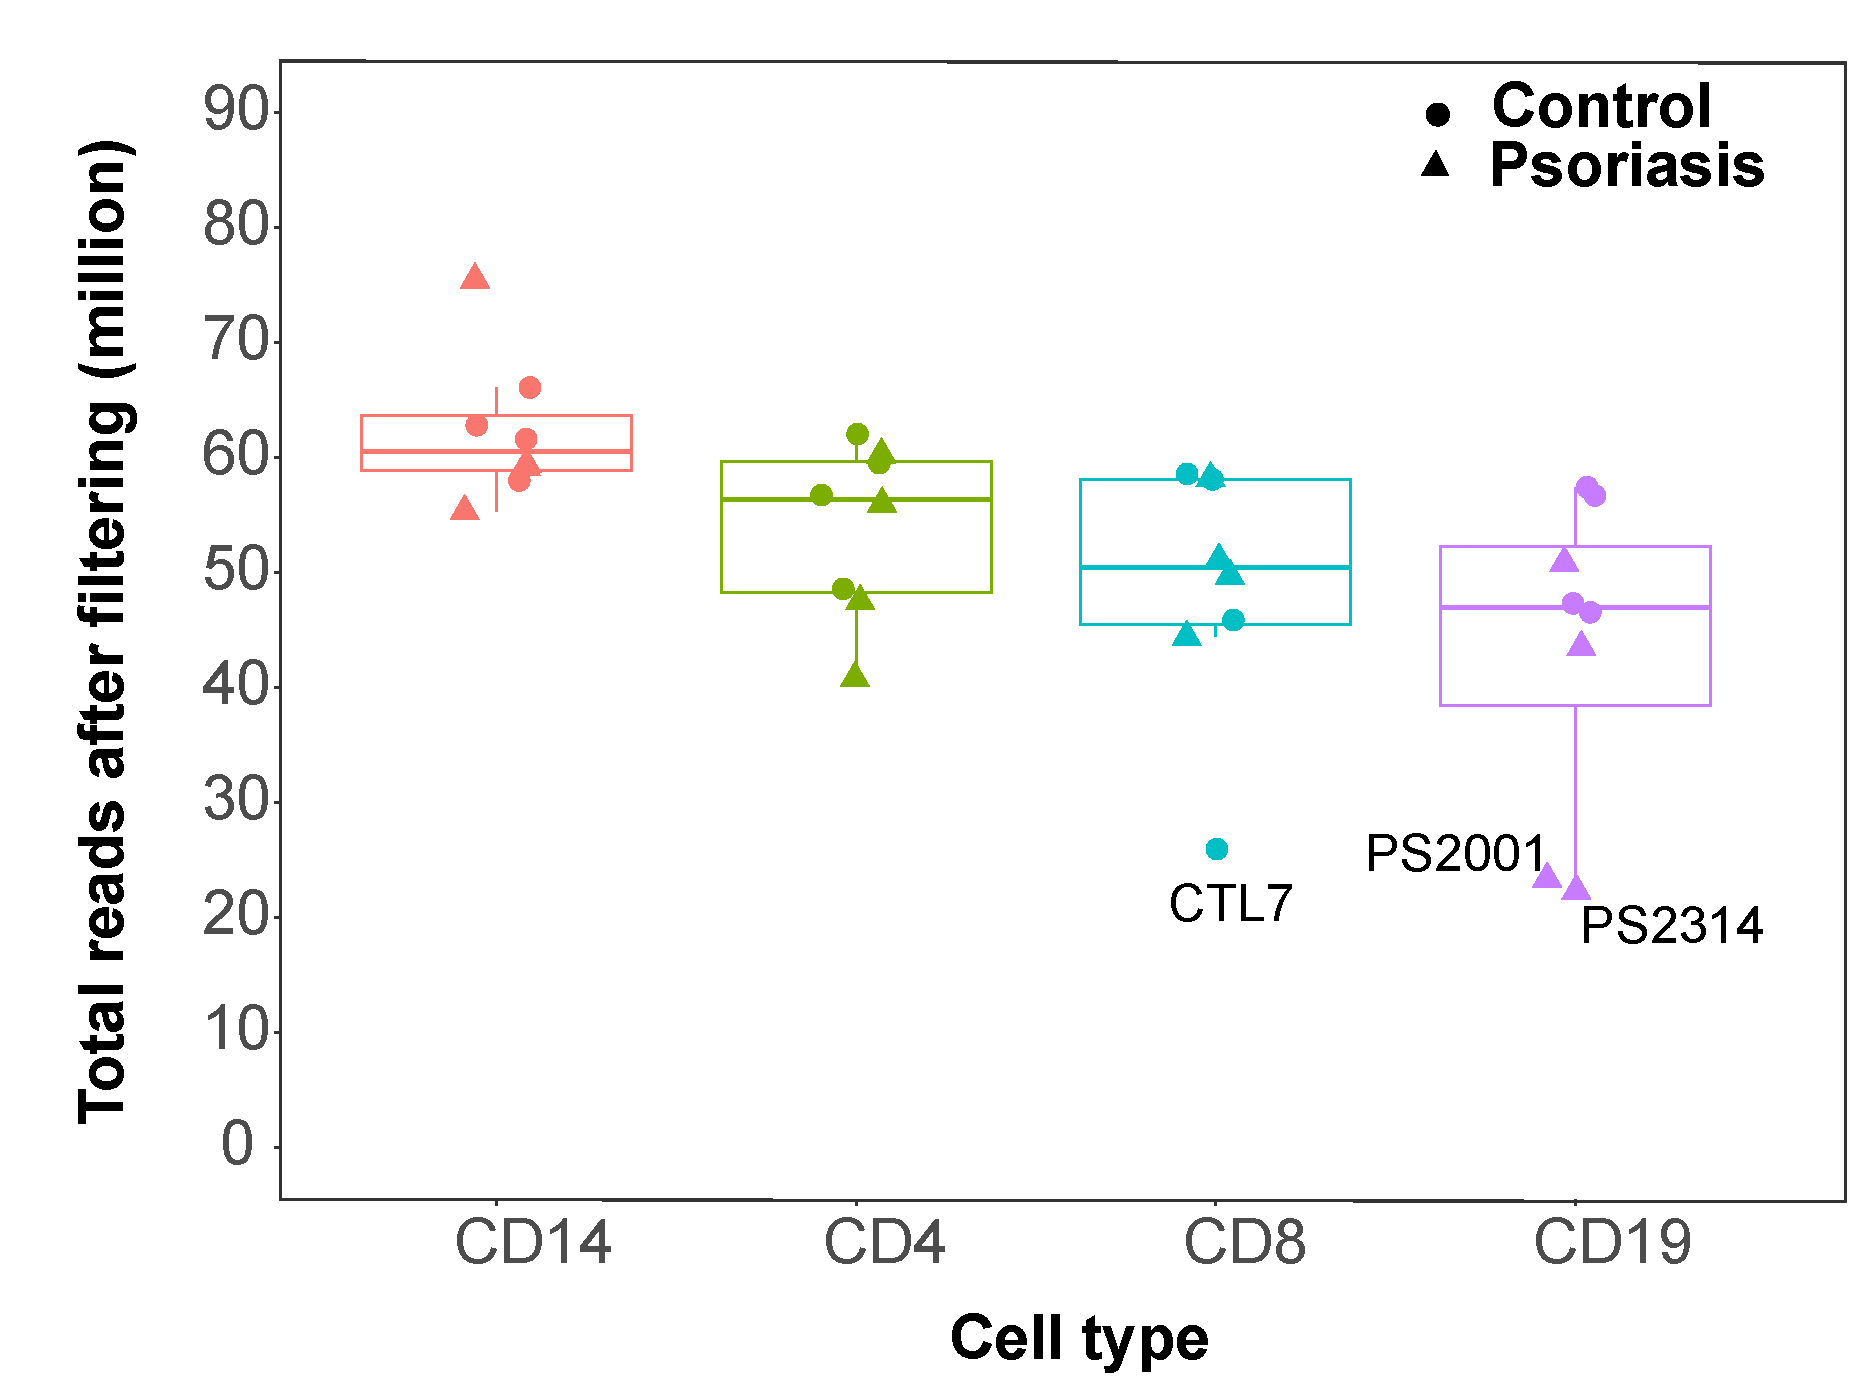
\includegraphics[width=\textwidth]{./Results2/pdfs/ChIPm_PS_CTL_final_filtered_reads_boxplot}
\caption{\textbf{}}
% The percentage sign indicated that the other subfig goes side by side
\end{subfigure} \\
\begin{subfigure}{0.5\textwidth}
\centering
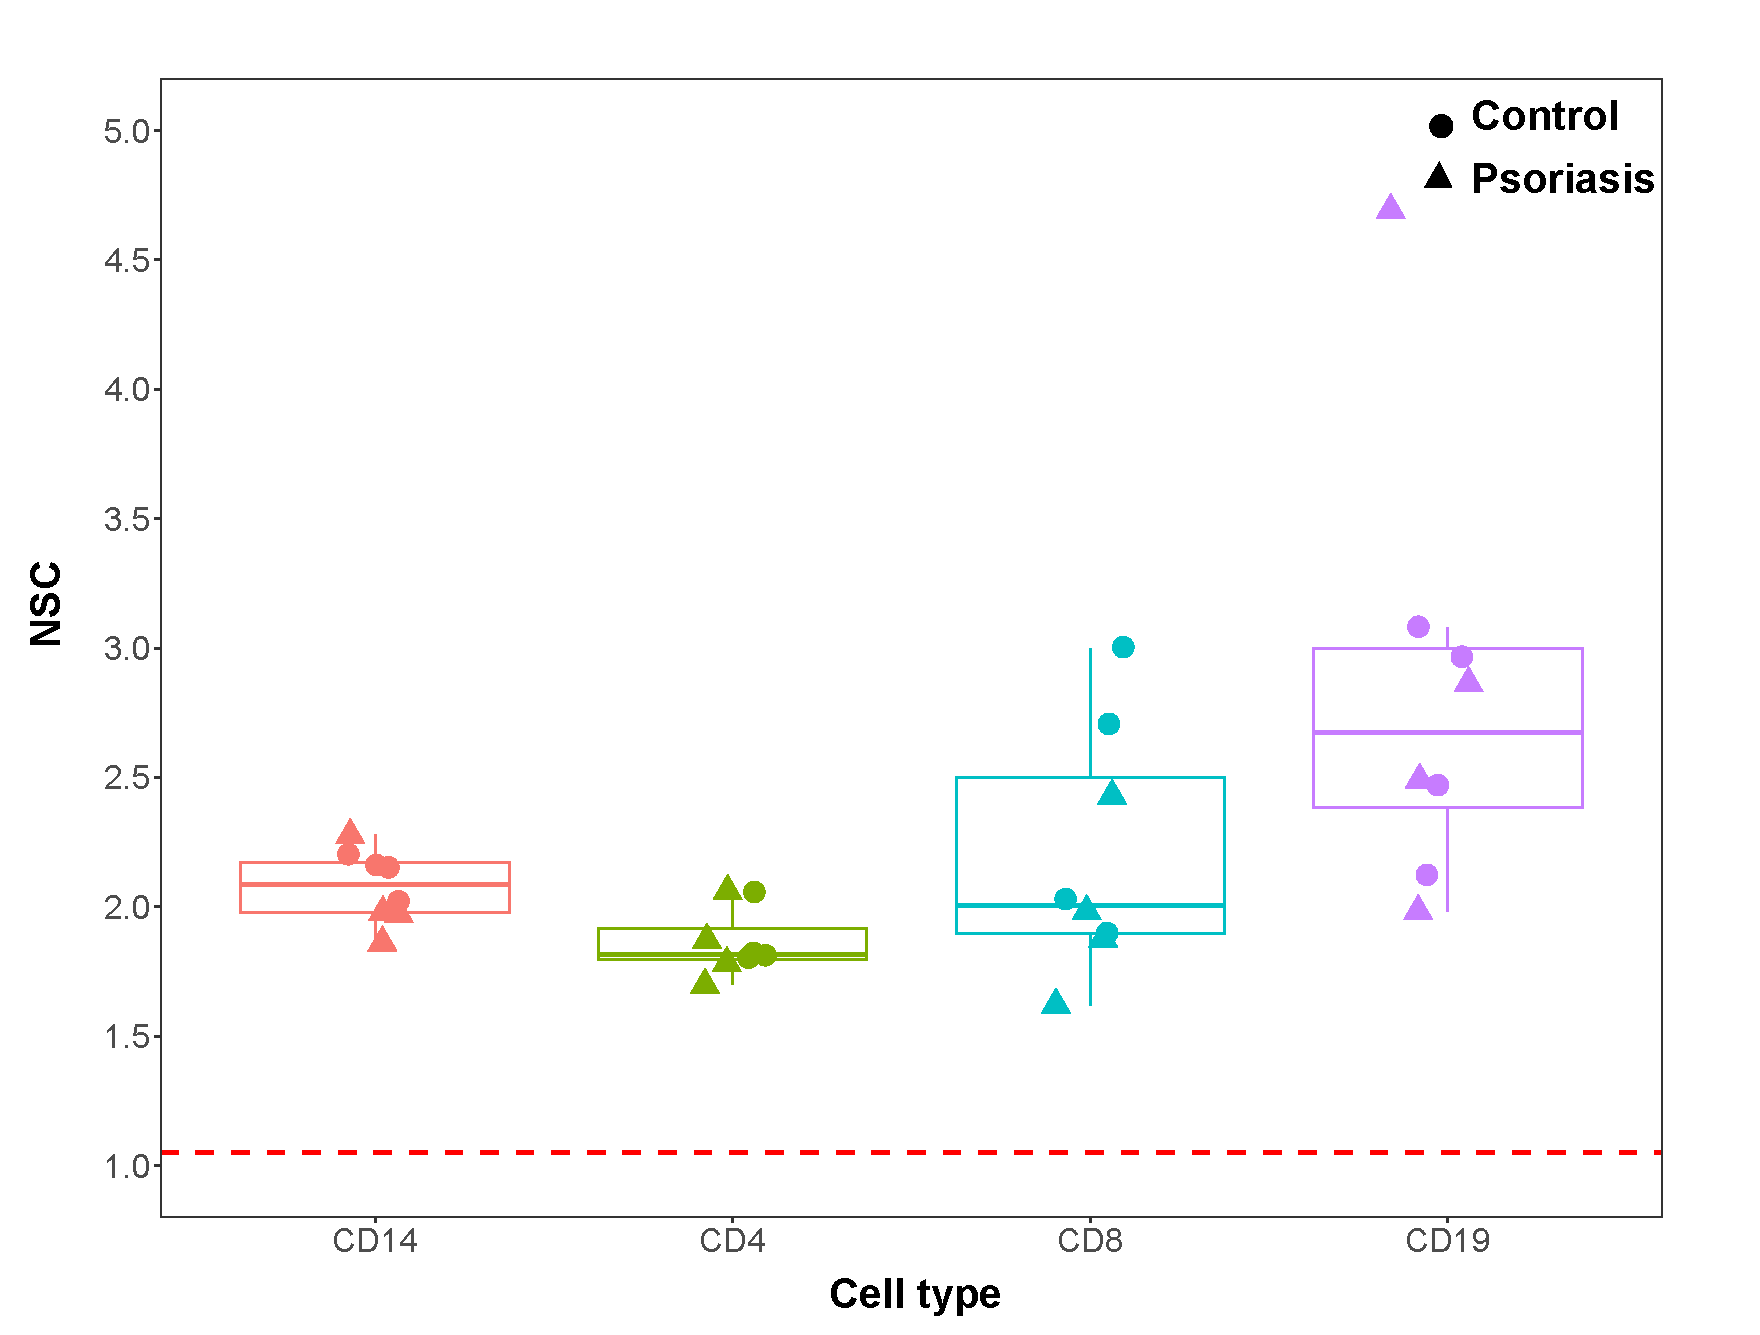
\includegraphics[width=\textwidth]{./Results2/pdfs/ChIPm_PS_CTL_NSC_boxplot}
\caption{\textbf{}}
\end{subfigure}%
\begin{subfigure}{0.5\textwidth}
\centering
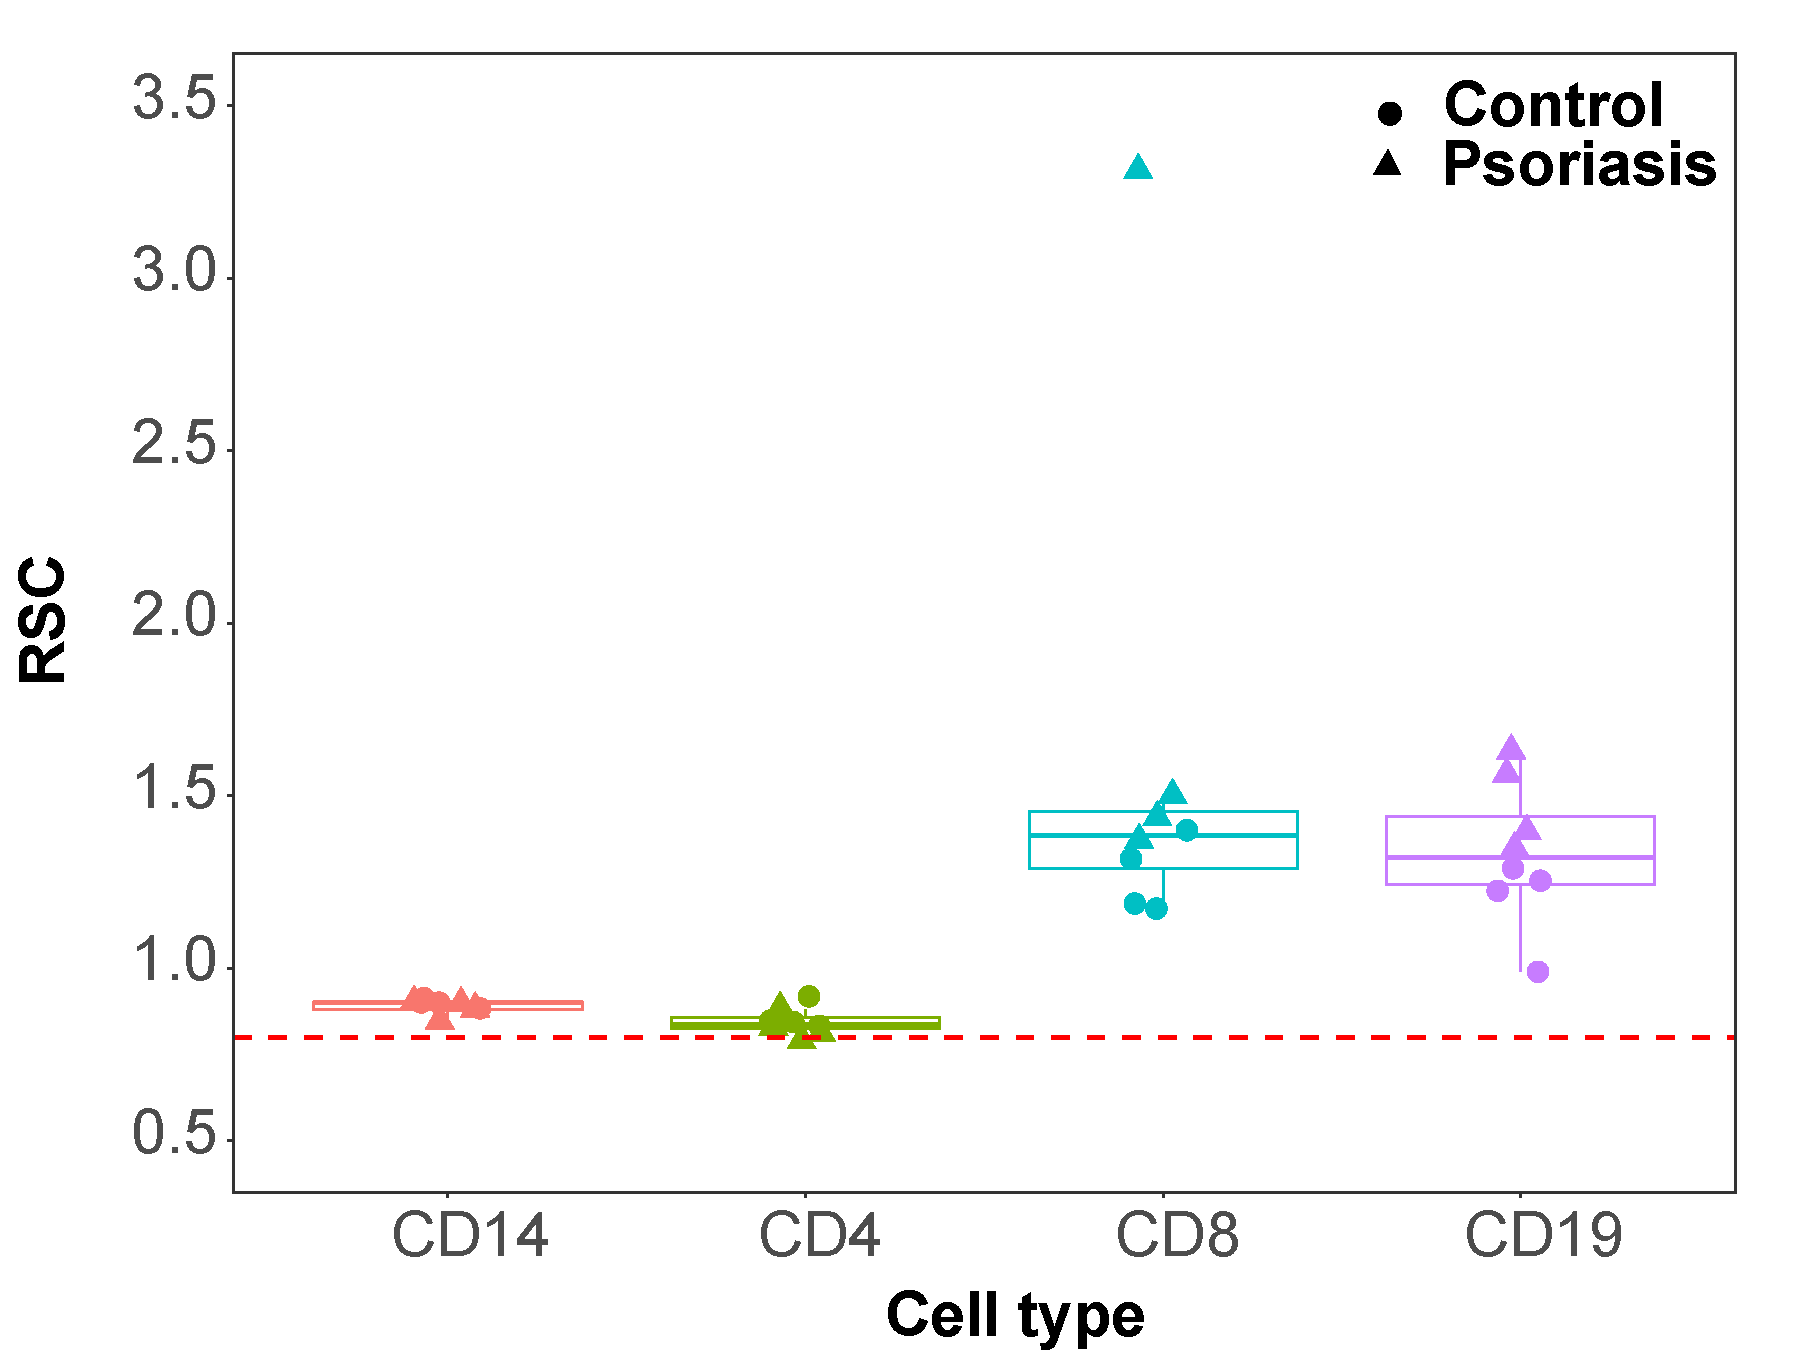
\includegraphics[width=\textwidth]{./Results2/pdfs/ChIPm_PS_CTL_RSC_boxplot}
\caption{\textbf{}}
\end{subfigure}
\caption[Quality control evaluation of the H3K27ac ChIPm libraries in immune cells isolated from psoriasis and control samples.]{\textbf{Quality control evaluation of the H3K27ac ChIPm libraries in immune cells isolated from psoriasis and control samples.} For each of the cell types boxplots representing a) million of reads after filtering, b) normalised strand cross-correlation coefficient (NSC) and c) relative strand cross-correlation coefficient (RSC). NSC and RSC are measures of signal enrichment independent of peak calling, where 1 and 0 indicate no enrichment, respectively. In c) and d) the dashed red line indicates the Encode threshold for low enrichment (NSC$<$1.05 and RSC$<$0.8). For each point, colour codes for cell type and shape for phenotype (psoriasis or control).}
\label{figure:ChIPm_PS_CTL_QC}
\end{figure} 




PCA analysis using a combined master list of the H3K27ac enriched sites in patients and controls for all four cell types (excluding the aforementioned low quality samples) confirmed the ability of this data to recapitulate the cell type specific epigenetic landscape of this enhancer mark and reinforced the appropriate quality of the data (Figure \ref{figure:ChIPm_PCA_and_chromatin_states} a). When performing PCA analysis by cell type, the PS2314 CD8$^+$ library appeared as an outlier compared to the rest of CD8$^+$ H3K27ac ChIPm patients and control libraries and was also removed for downstream analysis (data not shown). 

\bigskip
\begin{figure}[htbp]
\centering
\begin{subfigure}[b]{0.6\textwidth}
\centering 
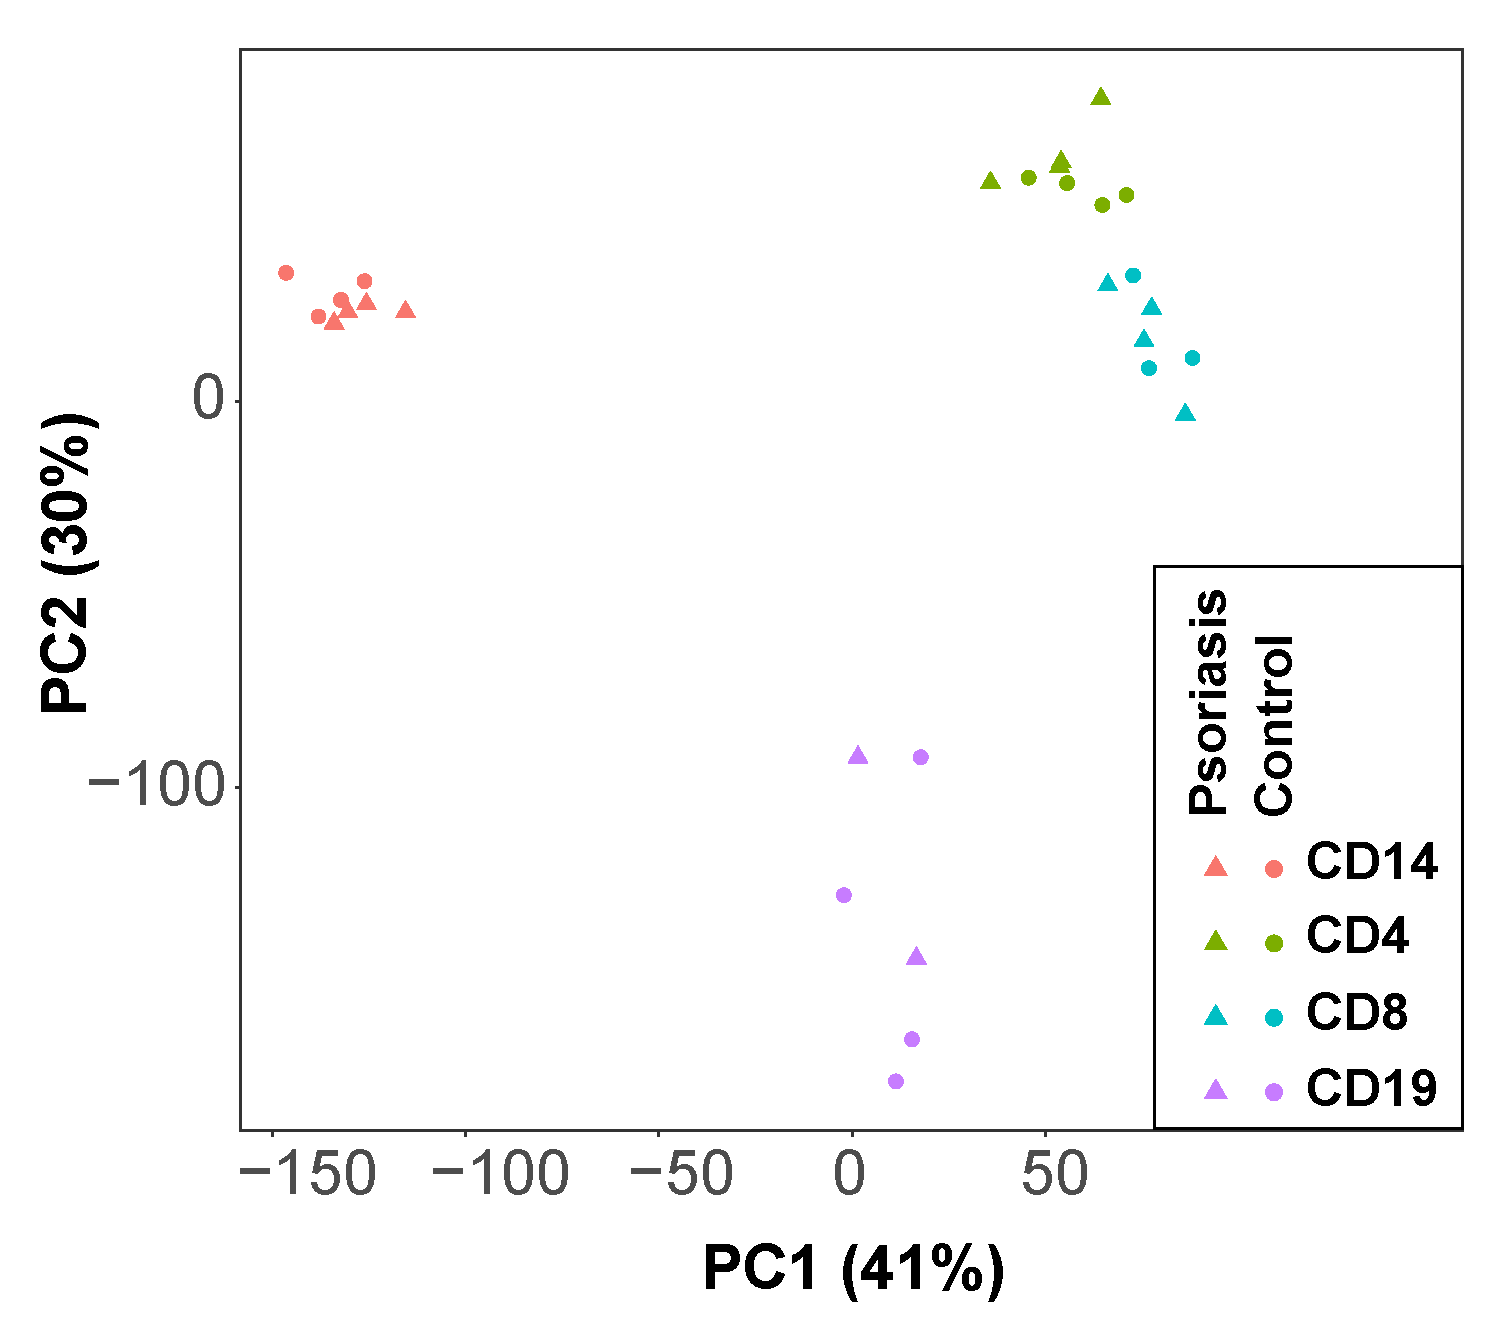
\includegraphics[width=\textwidth]{./Results2/pdfs/ChIPm_H3K27ac_all_cell_types_filtered_PCA}
\caption{}
\end{subfigure}
~
\begin{subfigure}[b]{0.6\textwidth} 
%the [b] prevents offset in subcaptions
\centering
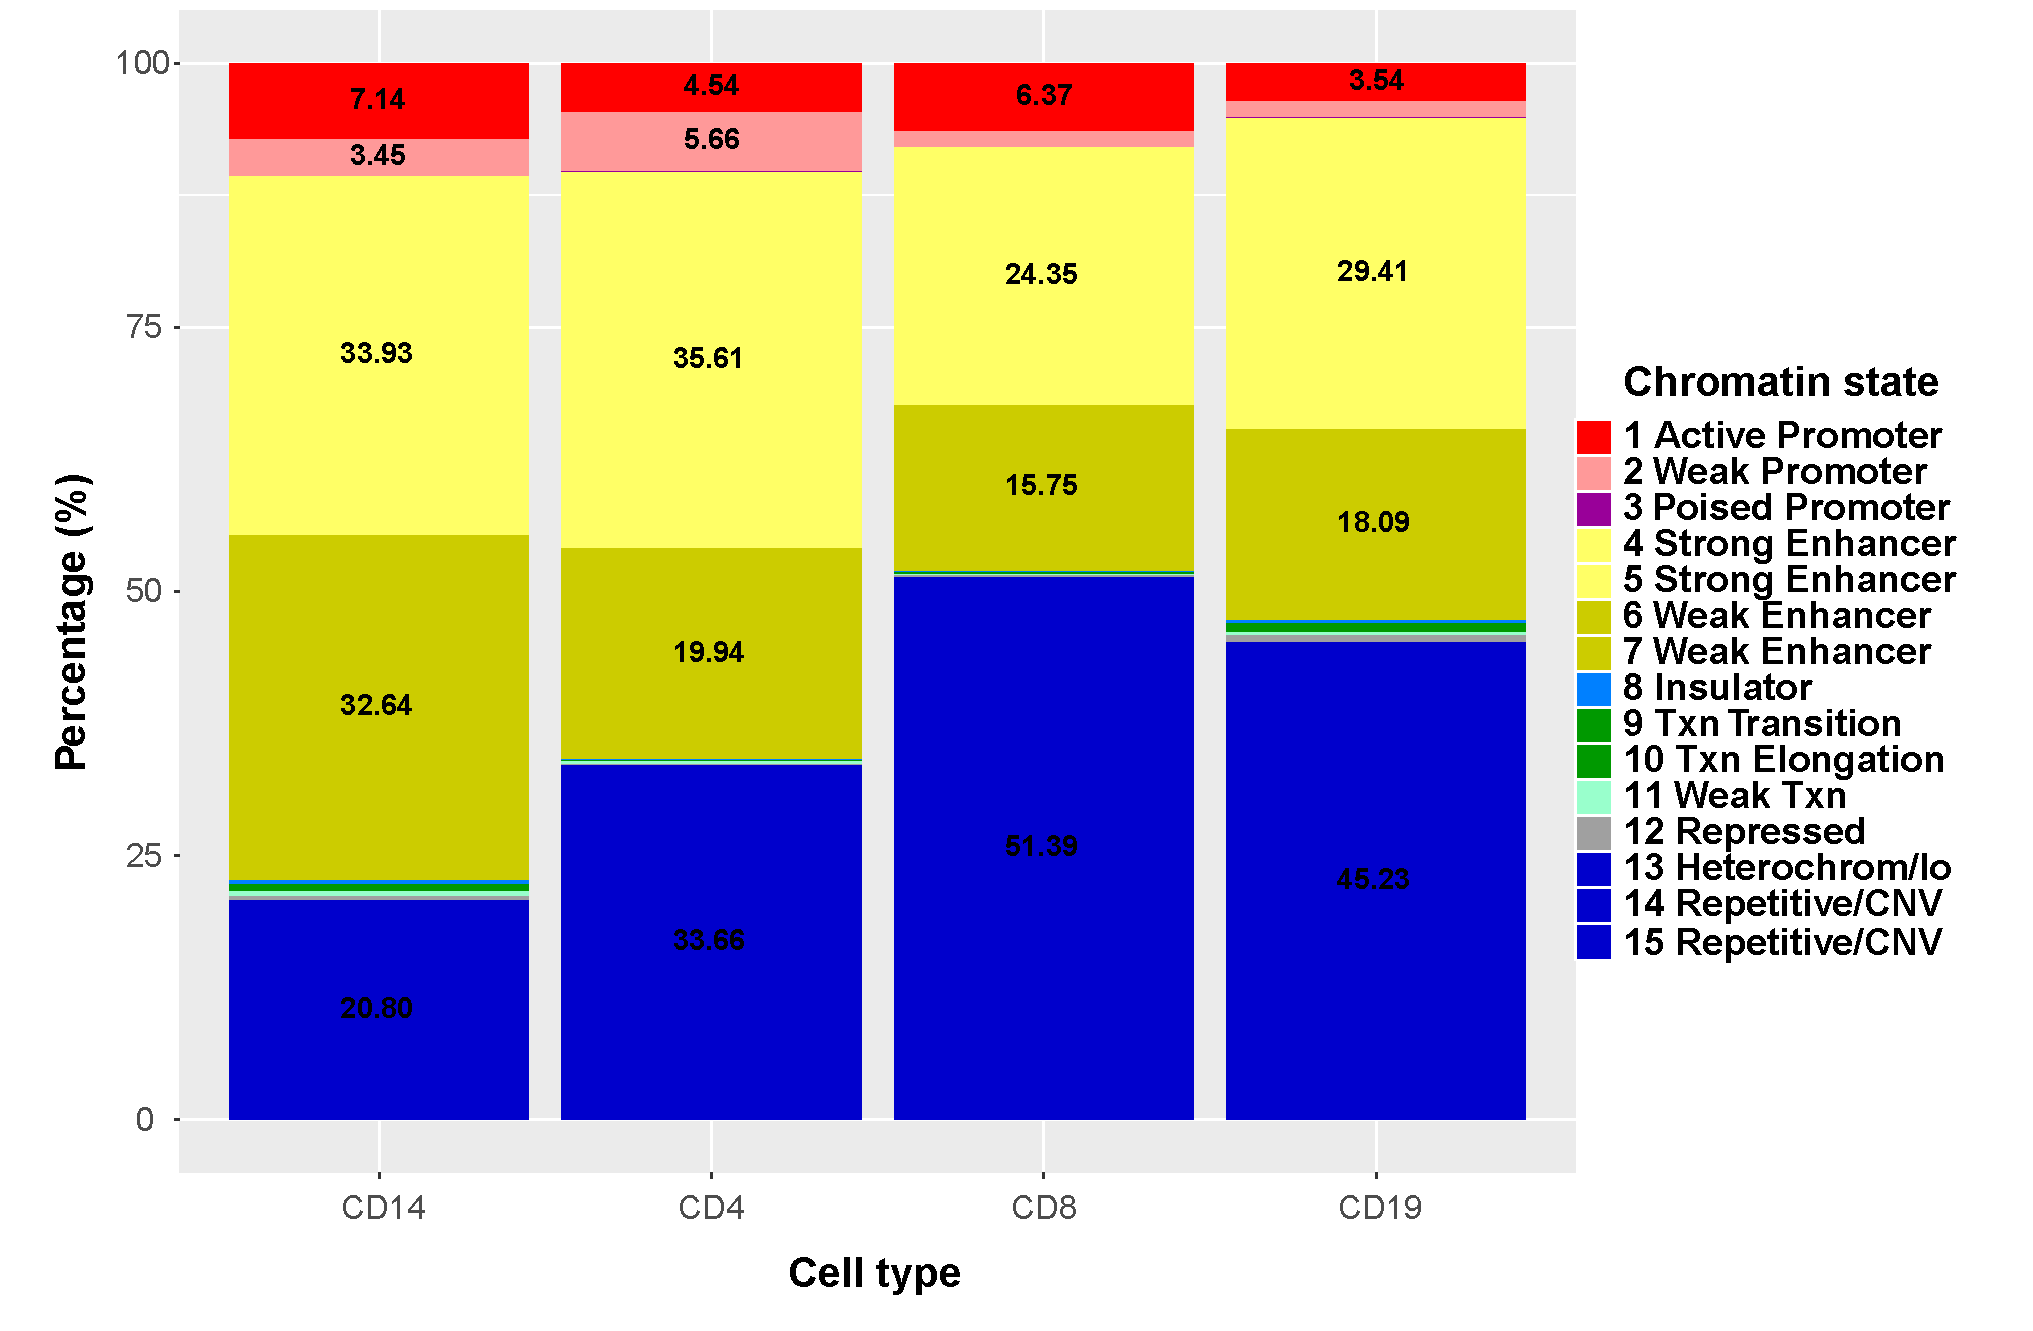
\includegraphics[width=\textwidth]{./Results2/pdfs/ChIPm_H3K27ac_cell_type_specific_master_list_chromatin_states_annotated_filtered}
\caption{}
\end{subfigure}
\caption[PCA analysis and chromatin annotation states of the H3K27ac enriched sites in four immune primary cell types from psoriasis and healthy control samples.]{\textbf{PCA analysis and chromatin annotation states of the H3K27ac enriched sites in four immune primary cell types from psoriasis and healthy control samples.} a) PCA analysis was performed using the normalised counts across a consensus master list of the combined H3K27ac enriched regions in psoriasis patients and healthy control samples across CD14$^+$ monocytes, CD4$^+$, CD8$^+$ and CD19$^+$ cells. The first two PCs (x-axis and y-axis, respectively) for all the H3K27ac ChIPm peaks in the master list are plotted. b) Annotation of the H3K27ac list of consensus enriched sites built by DiffBind for each cell was performed using the appropriate cell type specific RoadMap chromatin segmentation maps. Results are expressed as the percentage of regions annotated with a particular chromatin state over the total number of H3K27ac enriched sites in each individual cell type master list.}
\label{figure:ChIPm_PCA_and_chromatin_states}
\end{figure}


\subsubsection{Differential H3K27ac enrichment analysis}

Differential H3K27ac analysis was performed between psoriasis and healthy control samples for each cell type using DiffBind. The consensus merged list of H3K27ac sites assembled by this algorithm to perform the differential analysis (as explained in Chapter \ref{ch:Mat}) included a high percentage of sites annotated as heterochromatin or repetitive (Figure \ref{figure:ChIPm_PCA_and_chromatin_states} b), ranging from 20.8\% in CD14$^+$ monocytes to 51.39\% in tCD8$^+$ cells. Such sites are less likely to be relevant since H3K27ac is a histone modification mainly enriched at enhancers. When restricting the differential analysis to those regions annotated as enhancers (weak and strong), CD14$^+$ monocytes appeared as the cell type with the greatest number of differentially modified enhancers (8 significant sites), followed by CD4$^+$ (4) and CD8$^+$ (1) (Table \ref{tab:ChIPm_differential_analysis_results}).



\begin{table}[htbp]
%\setlength{\tabcolsep}{20pt} only to stretch the columns if you want
%\renewcommand{\arraystretch}{1.5}
\centering
\begin{tabular}{@{} c c c}
\toprule
\textbf{Cell type}   & \textbf{Master list size}      & \textbf{Differential regions}      \\
                     & \textbf{genome-wide/enhancers} & \textbf{genome-wide/enhancers}     \\
\midrule
\midrule
CD14$^+$             & 99,862/60,962                  & 15/8                                \\
tCD4$^+$              & 110,353/56,282                 & 0/4																	\\
tCD8$^+$              & 137,194/51,607                 & 8/1                                 \\ 
CD19$^+$             & 199,014/88,722                 & 12/0                                 \\
\bottomrule 
\end{tabular}
\medskip %gap
\caption[Summary results from the differential H3K27ac analysis between psoriasis patients and healthy controls in CD14$^+$ monocytes, CD4$^+$, CD8$^+$ and CD19$^+$ cells.]{\textbf{Summary results from the differential H3K27ac analysis between psoriasis patients and healthy controls in CD14$^+$ monocytes, CD4$^+$, CD8$^+$ and CD19$^+$ cells.} In the genome-wide analysis, the master list size refers to the number of H3K27ac enriched sites included in the consensus list built using DiffBind to perform the differential analysis. In the analysis restricted to enhancers, the size of the master list was reduced to only those sites from the genome-wide master list annotated as enhancers (weak and strong) according to the chromatin segmentation map for each particular cell type. Genome-wide significant sites in CD14$^+$ monocytes and CD8$^+$ also contain the sites identified in the enhancer restricted analysis. Significant differentially H3K27ac modified regions were determined using FDR$<$0.05 and no FC threshold.}
\label{tab:ChIPm_differential_analysis_results}
\end{table}
\bigskip %bigger space


One of the differentially H3K27ac modified regions when comparing patients versus controls in CD14$^+$ monocytes was located between the \textit{SLC15A2} and \textit{ILDR2} genes, where \textit{ILDR2} has recently been identified as relevant for negative regulation of T cells response in RA \parencite{Hecht2018}. This region presented lower H3K27ac levels in psoriasis patients compared to controls and was annotated as enhancer by the Epigenome Roadmap chromatin segmentation map (Figure \ref{figure:ChIPm_H3K27ac_UCSC_ILDR1_track}). Additionally this site was overlapping a DHS and H3Kme1 (enhancer mark) modification and a CTCF-binding site identified by ChIP-seq in K562 cells. Pblicly available chromatin conformation data in T cells failed to show interactions of this region with the promoter of any of the proximal genes in monocytes and eQTL data has suggested regulation of the calmodulin-binding motif-containing protein \textit{IQCB1} gene in monocytes and tCD4$^+$ cells \parencite{GTeX,Fairfax2014, Kasela2017}. Amongst the tCD4$^+$ hits, all the significant regions presented minor changes with no evidence of regulating expression of any relevant gene by proximity or based on chromatin conformation data. 


%Conversely, this region harbours SNPs that have been identified as \textit{cis}-eQTL in whole blood and total unstimulated and stimulated CD14$^+$ monocytes for the calmodulin-binding motif-containing protein \textit{IQCB1} gene, which is 186.4Kb up-stream of this peak \parencite{GTeX,Fairfax2014}. MS risk LD SNPs (rs34543553, rs73855480 and rs73855480) in this peak are also \textit{cis}-eQTLs in unstimulated total CD4$^+$ and CD8$^+$ cells for \textit{IQCB1} \parencite{Kasela2017}. 



\begin{figure}[htbp]
\centering
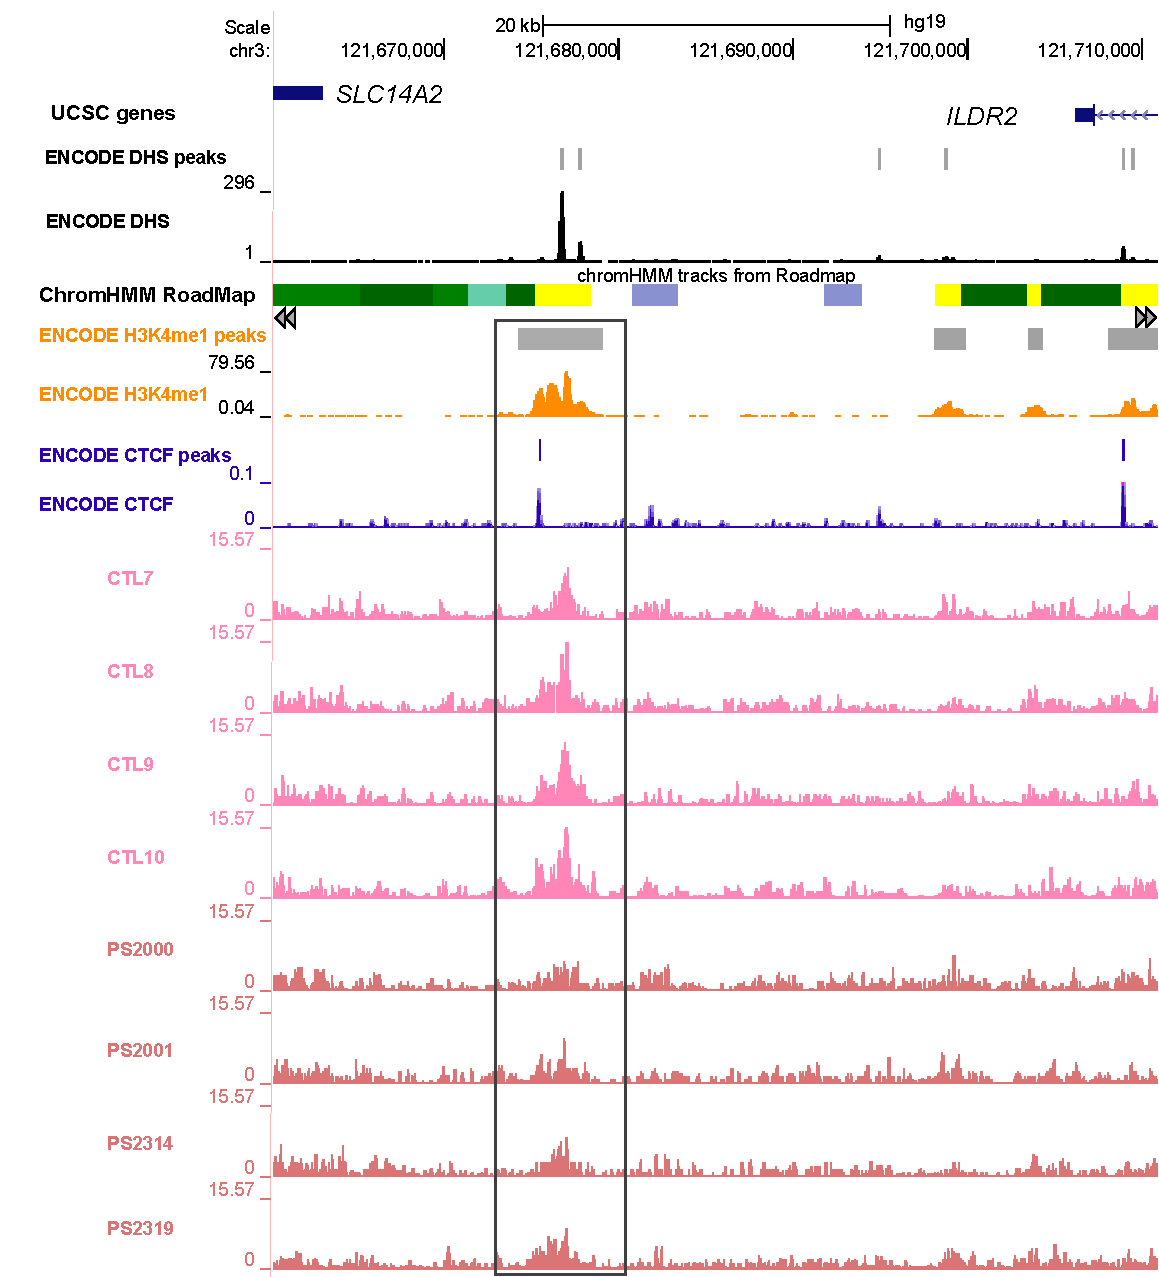
\includegraphics[width=0.6\textwidth]{./Results2/pdfs/ChIPm_H3K27ac_UCSC_CD14_ILDR1_track}
\caption[Differential H3K27ac modification at a putative intergenic enhancer region in circulating CD14$^+$ monocytes between psoriasis patients and healthy controls.]{\textbf{Differential H3K27ac modification at a putative intergenic enhancer region in circulating CD14$^+$ monocytes between psoriasis patients and healthy controls.} UCSC Genome Browser view illustrating the normalised H3K27ac fold-enrichment (y-axis) at an intergenic differentially modified region located between \textit{SLC14A2} and \textit{ILDR2} genes (x-axis) in CD14$^+$ monocytes (lower H3K27ac enrichment in psoriasis patients compared to healthy controls). CD14$^+$ monocytes publicly available epigenetic data from ENCODE (including DHS, H3K4me1 and CTCF ChIP-seq) and the Epigenome Roadmap chromatin segmentation track are also shown. Differential H3K27ac modified regions were considered significant based on FDR$<$0.05 and no FC cut-off. H3K27ac tracks are colour-coded by condition: control(CTL)=pink and psoriasis (PS)=sienna.}
\label{figure:ChIPm_H3K27ac_UCSC_ILDR1_track}
\end{figure}



When performing genome-wide differential analysis, CD14$^+$ monocytes and CD8$^+$ revealed additional statistically significant differentially H3K27ac modified regions, as well as those already identified in the restricted enhancer analysis (Table \ref{tab:ChIPm_differential_analysis_results}). The newly identified regions in both cell types were mostly in regions lacking DHS and  H3K4me1 modifications. Genome-wide analysis in CD4$^+$ cells did not reveal significant differentially modified targets outside enhancers and also failed to retain significance for the four hits identified in the restricted analysis, most likely due to increase in multiple testing as a result of the larger size of the master list (Table \ref{tab:ChIPm_differential_analysis_results}). The differential regions between psoriasis patients and controls identified in CD19$^+$ cells when performing genome-wide analysis presented considerable fold changes (absolute log$_2$FC ranging from 2.47 to 6.37). However, most of them (10 out of 12) did not overlap accessible chromatin and none were found to be interacting with other enhancers or distal promoters. The  absence of differentially H3K27ac sites between patients and controls at CD19$^+$ enhancers may reinforce the limited relevance for B cells in psoriasis when compared to the other three cell types.

Overall, restricting the differential analysis to enhancer annotated regions did not show a great increase in the number of significant differentially modified H3K27ac sites when compared to the genome-wide analysis in any of the four cell types. The results in this pilot cohort did not show relevant global epigenetic changes in H3K27ac sites between psoriasis patients and controls for these cell types and sample size.


\subsection{Identifying global changes in immune cells chromatin accessibility between psoriasis patients and healthy controls}

The cell type specific chromatin accessibility landscape is determined by the combination of histone modifications and DNA binding proteins (including TF and co-regulatory proteins) in a particular locus. The previous results showing only moderate changes in the H3K27ac landscape between patients and controls are not necessarily representative of the overall changes in the chromatin accessibility landscape in disease. In order to interrogate genome-wide changes in chromatin accessibility between patients and controls, ATAC-seq was performed in the same four cell types in eight patients and ten controls (Table \ref{tab:Psoriasis_controls_datasets_per_sample}) giving a total of 72 libraries.


\subsubsection{Data processing and quality control}
ATAC-seq quality control first found that the median total reads after filtering ranged between 39.2 and 49.8 in CD4$^+$ and CD19$^+$ respectively, and was over the 15 million reads determined as appropriate an minimum (Chapter \ref{ch:Results1}) in all the samples (Figure \ref{figure:ATAC_PS_CTL_QC} a). 


\begin{figure}[htbp]
\centering
\begin{subfigure}{0.5\textwidth}
\centering
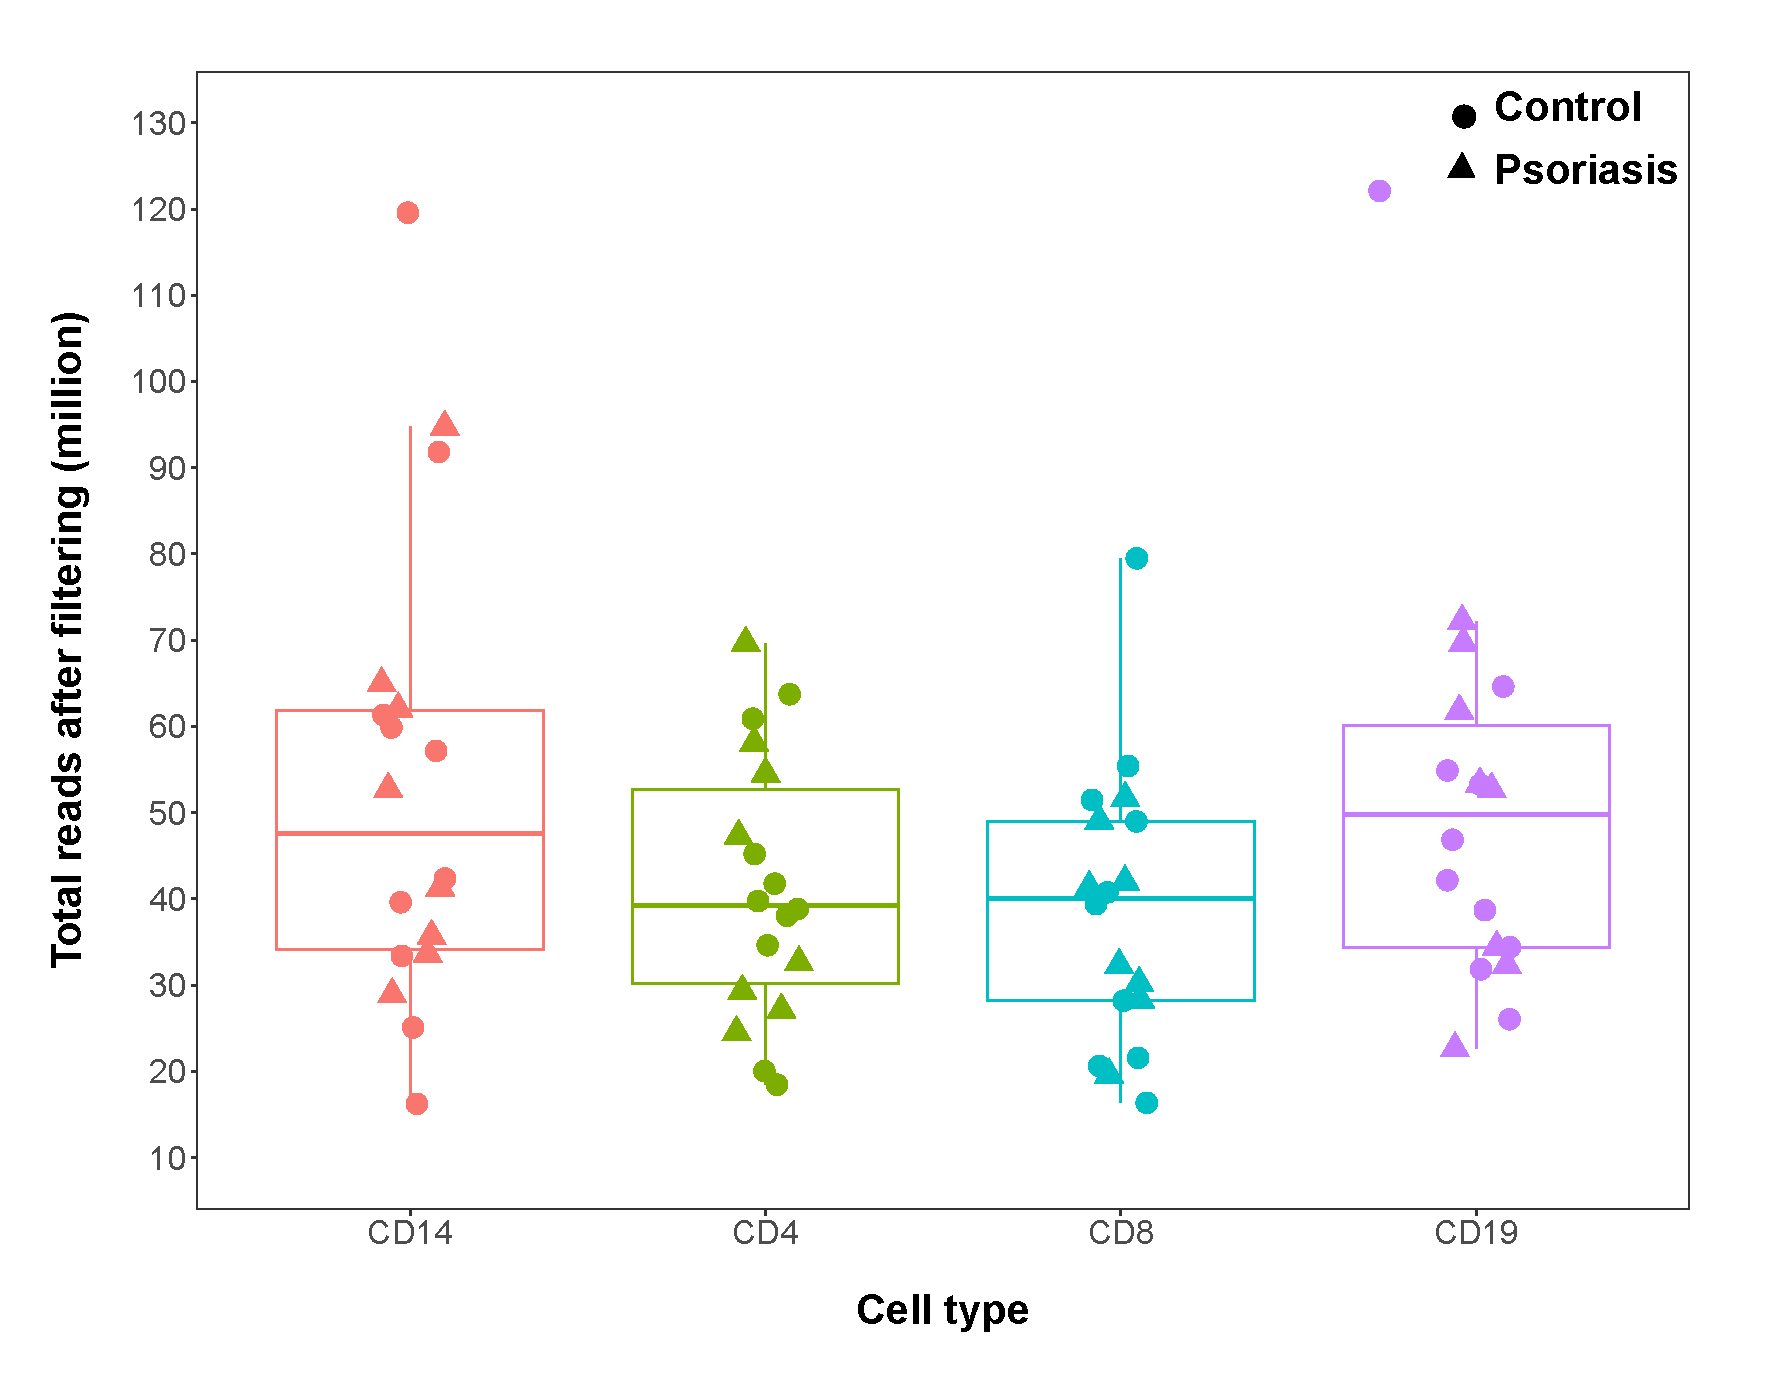
\includegraphics[width=\textwidth]{./Results2/pdfs/ATAC_PS_CTL_final_filtered_reads_boxplot}
\caption{\textbf{}}
% The percentage sign indicated that the other subfig goes side by side
\end{subfigure}%
\begin{subfigure}{0.5\textwidth}
\centering
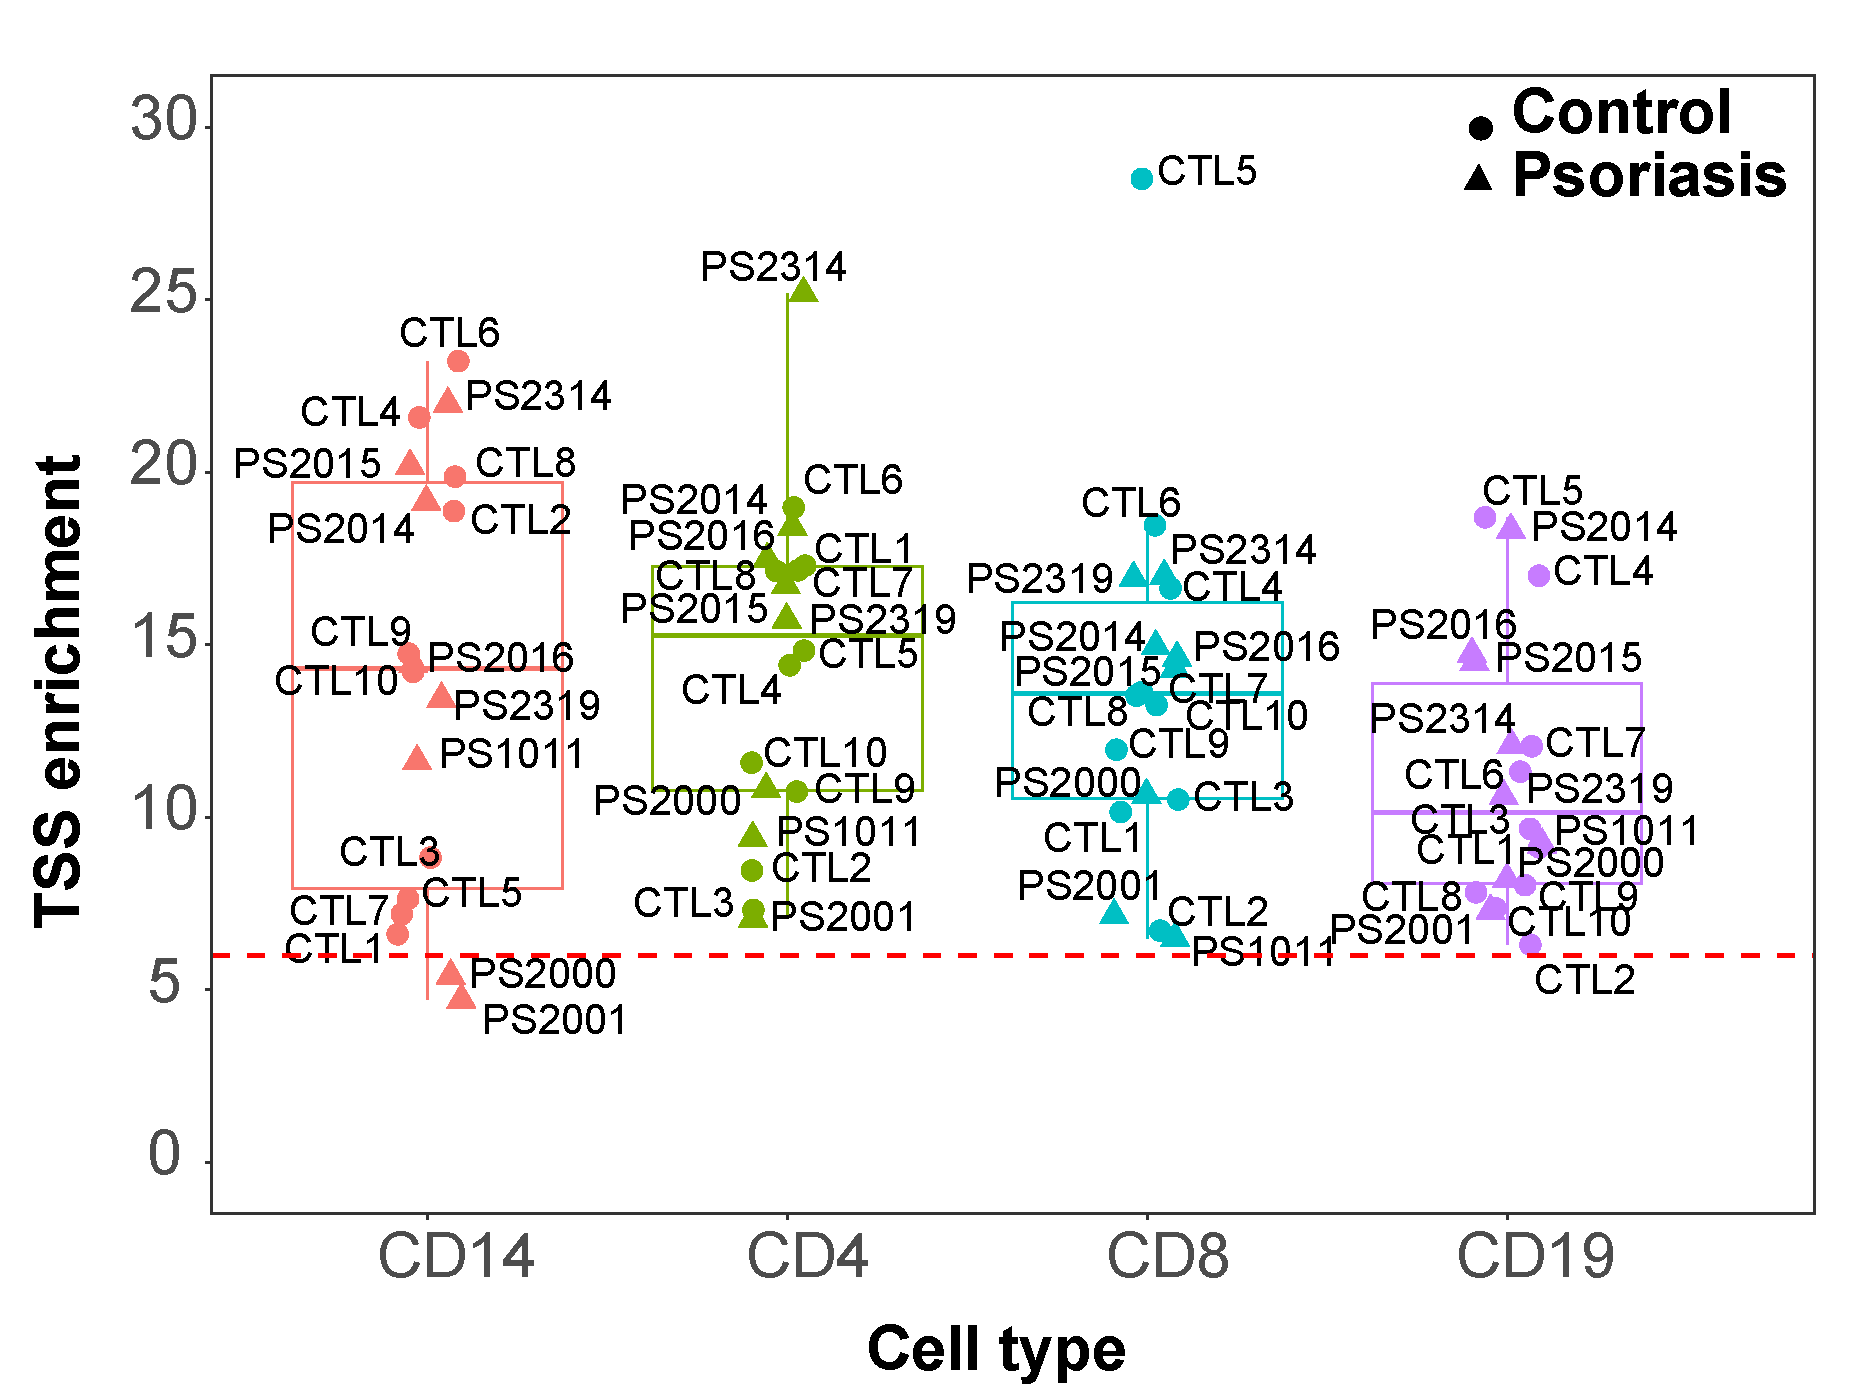
\includegraphics[width=\textwidth]{./Results2/pdfs/ATAC_PS_CTL_all_samples_TSS_boxplots_all_labelled}
\caption{\textbf{}}
\end{subfigure}
\begin{subfigure}{0.5\textwidth}
\centering
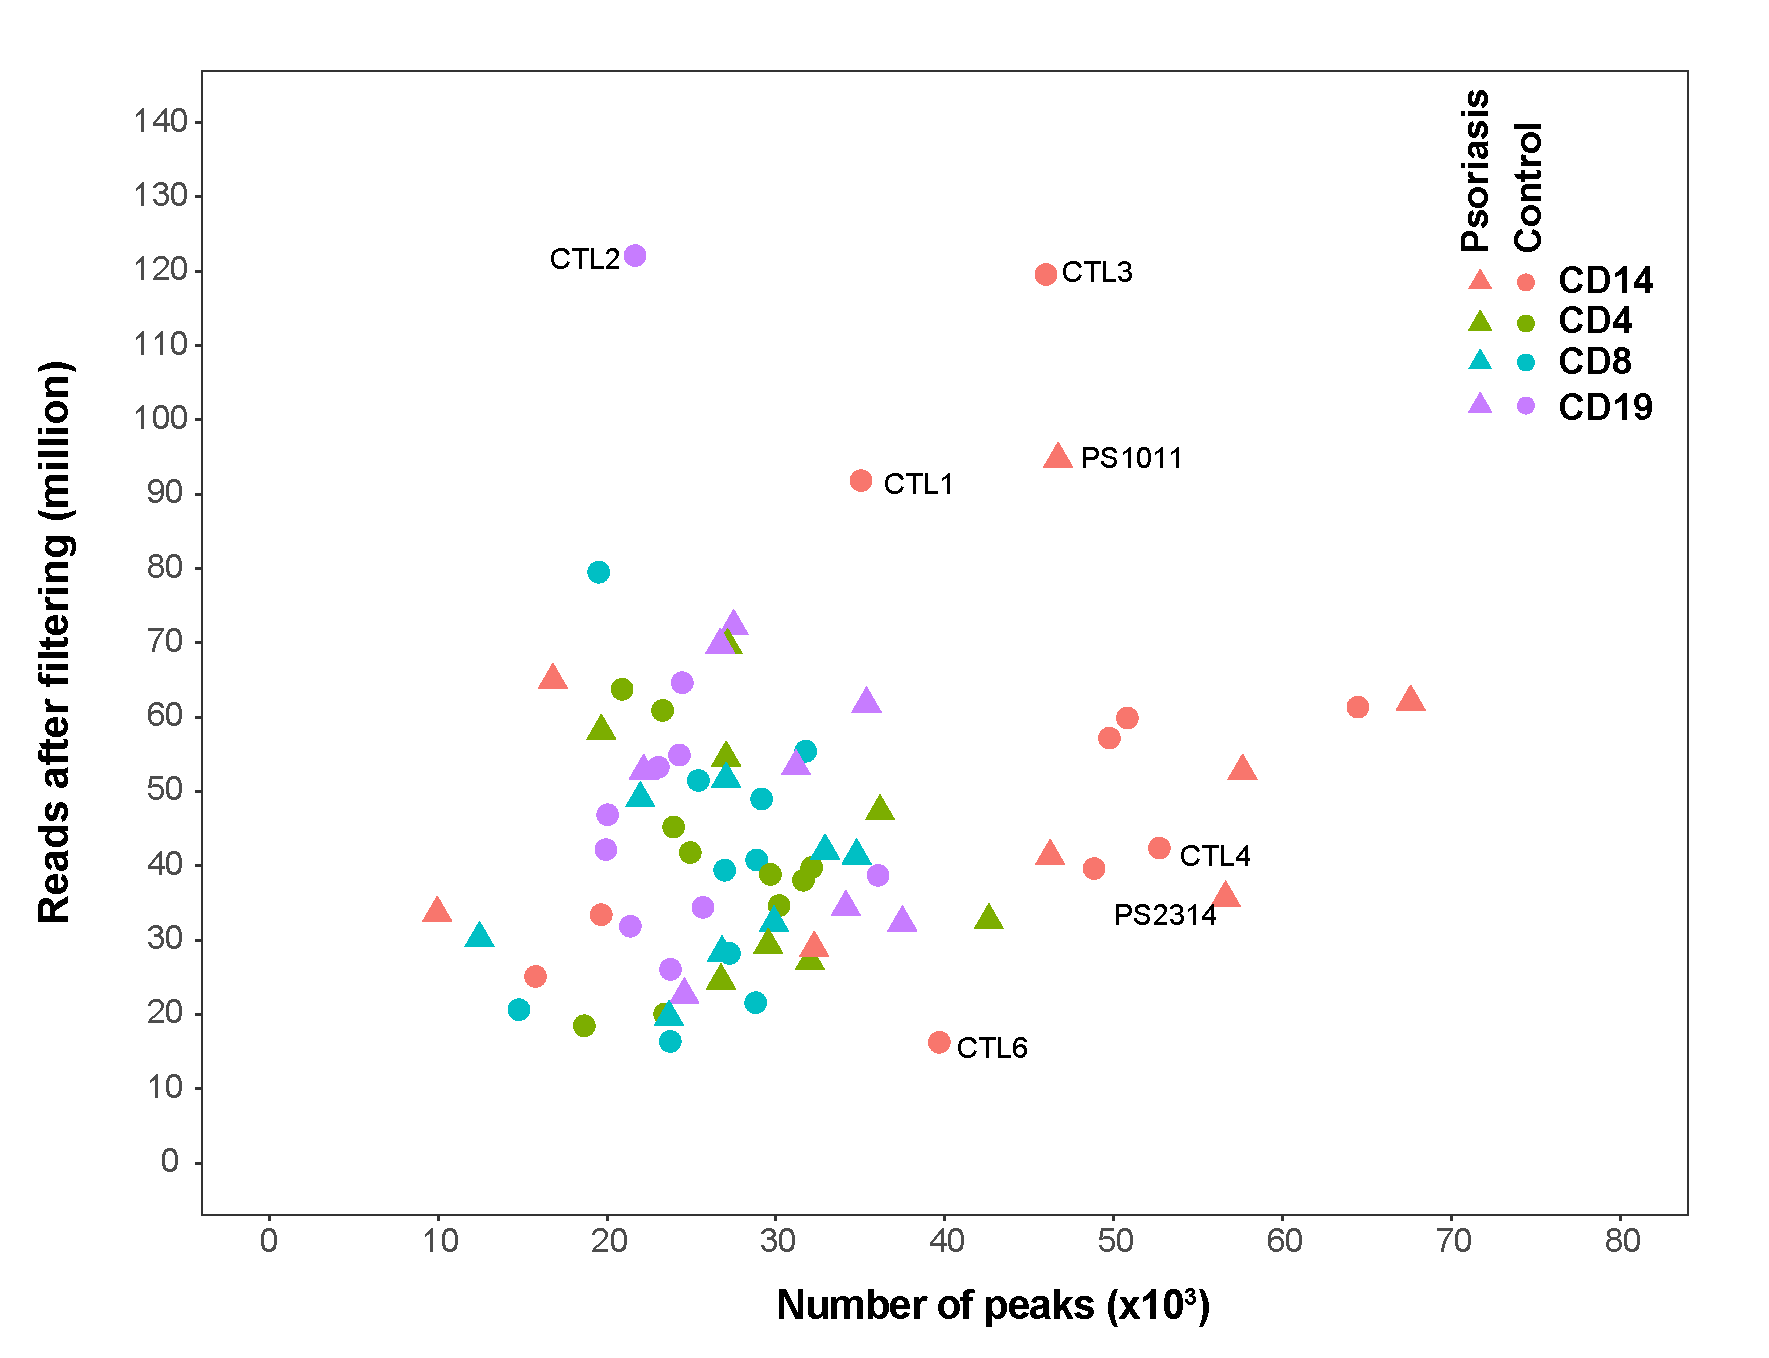
\includegraphics[width=\textwidth]{./Results2/pdfs/ATAC_PS_CTL_reads_vs_peaks_dotplot}
\caption{\textbf{}}
\end{subfigure}
\caption[Quality control assessment of the ATAC libraries generated from circulating immune cells in psoriasis and control samples.]{\textbf{Quality control assessment of the ATAC libraries generated from circulating immune cells in psoriasis and control samples.} For each of the cell types and samples, boxplots representing a) million of reads after filtering, b) values for fold-enrichment of ATAC fragments across the Ensembl annotated TSS and c) representation of the  number of significant peaks based on IDR optimal pval versus the total million reads after filtering for each of the samples. In b) the dashed red line indicates the recommended Encode threshold for TSS enrichment values. For each point, colour codes for cell type and shape for phenotype (psoriasis or control). In b) and c) sample IDs are included for all or some of the samples.}
\label{figure:ATAC_PS_CTL_QC}
\end{figure} 


The differences in read depths across ATAC samples are mostly due to intrinsic difficulties in determining molarity of the ATAC libraries (due to the fragment size heterogeneity) as well as the number of duplicates present in each library, which also correlated with MT reads. Differences in the percentage of MT reads were noticeable between samples from cohort 1A generated with the standard ATAC-seq protocol from Buenrostro \textit{et al.}, 2013 and the Fast-ATAC libraries from cohort 1B using the later modified \parencite{Corces2016} protocol (Figure \ref{figure:ATAC_PS_CTL_MT_percent}). 

All the samples showed the required characteristic ATAC-seq fragment size distribution recapitulating nucleosome periodicity (data not shown) (previously detailed in Chapter \ref{ch:Results1}). Analysis of ATAC-seq signal enrichment across gene TSSs revealed that most of the samples had enrichment over 6 (Figure \ref{figure:ATAC_PS_CTL_QC} b) and only PS2000 and PS2001 CD14$+$ monocytes were removed from downstream analysis due to low signal-to-noise ratios ($<$6). When comparing the number of peaks passing IDR filtering in each samples versus the number of reads after filtering, most of the samples presented between 10,000 and 35,000 peaks (Figure \ref{figure:ATAC_PS_CTL_QC} c). Since the sequencing depth of most of the samples was $\geq$15 million reads, most of the differences in number of called peaks were intrinsic to the cell type and the signal-to-noise differences in the samples, as previously studied in Chapter \ref{ch:Results1}. For example, CD14$^+$ monocytes had greater numbers of peaks when compared to the other three cell types, despite the median total number of reads after filtering being similar to the other cell types (Figure \ref{figure:ATAC_PS_CTL_QC} a). %Also, within the CD14$^+$ monocytes samples, those with the greatest TSS fold-enrichment (e.g CTL4, CTL6 and PS2314) presented similar numbers of good quality called peaks to the samples with higher numbers of reads after filtering and lower signal-to-noise ratios (e.g  PS1011, CTL1 and CTL3) (Figure \ref{figure:ATAC_PS_CTL_QC} a and c). 
CD19$^+$ CTL2 appeared to be an outlier, with a noticeably lower number of peaks for its high sequencing depth (Figure \ref{figure:ATAC_PS_CTL_QC} c). This observation together with its border line TSS enrichment supported removal of the CD19$^+$ CTL2 sample from downstream analysis.


\subsubsection{Functional relevance of the ATAC regions included in the differential analysis}

A heatmap illustrating sample distance using the consensus master list of ATAC-seq regions across the four cell types (ML\_all) showed successful separation of the samples according to the cell type into three main clusters corresponding to CD14$^+$ monocytes, CD19$^+$ and CD4$+$/CD8$^+$ T cells (Figure \ref{figure:ATAC_PS_CTL_heatmap_TFBS} a). Within each of the cell type clusters, samples did not separate based on disease condition, suggesting the absence of large global differences in the chromatin accessibility landscape between psoriasis patients and control individuals. Conversely, within the cell types there was some grouping of samples by batch (Figure \ref{figure:ATAC_PS_CTL_heatmap_TFBS} a).

\bigskip
\begin{figure}[H]
\centering
\begin{subfigure}[b]{0.5\textwidth}
\centering 
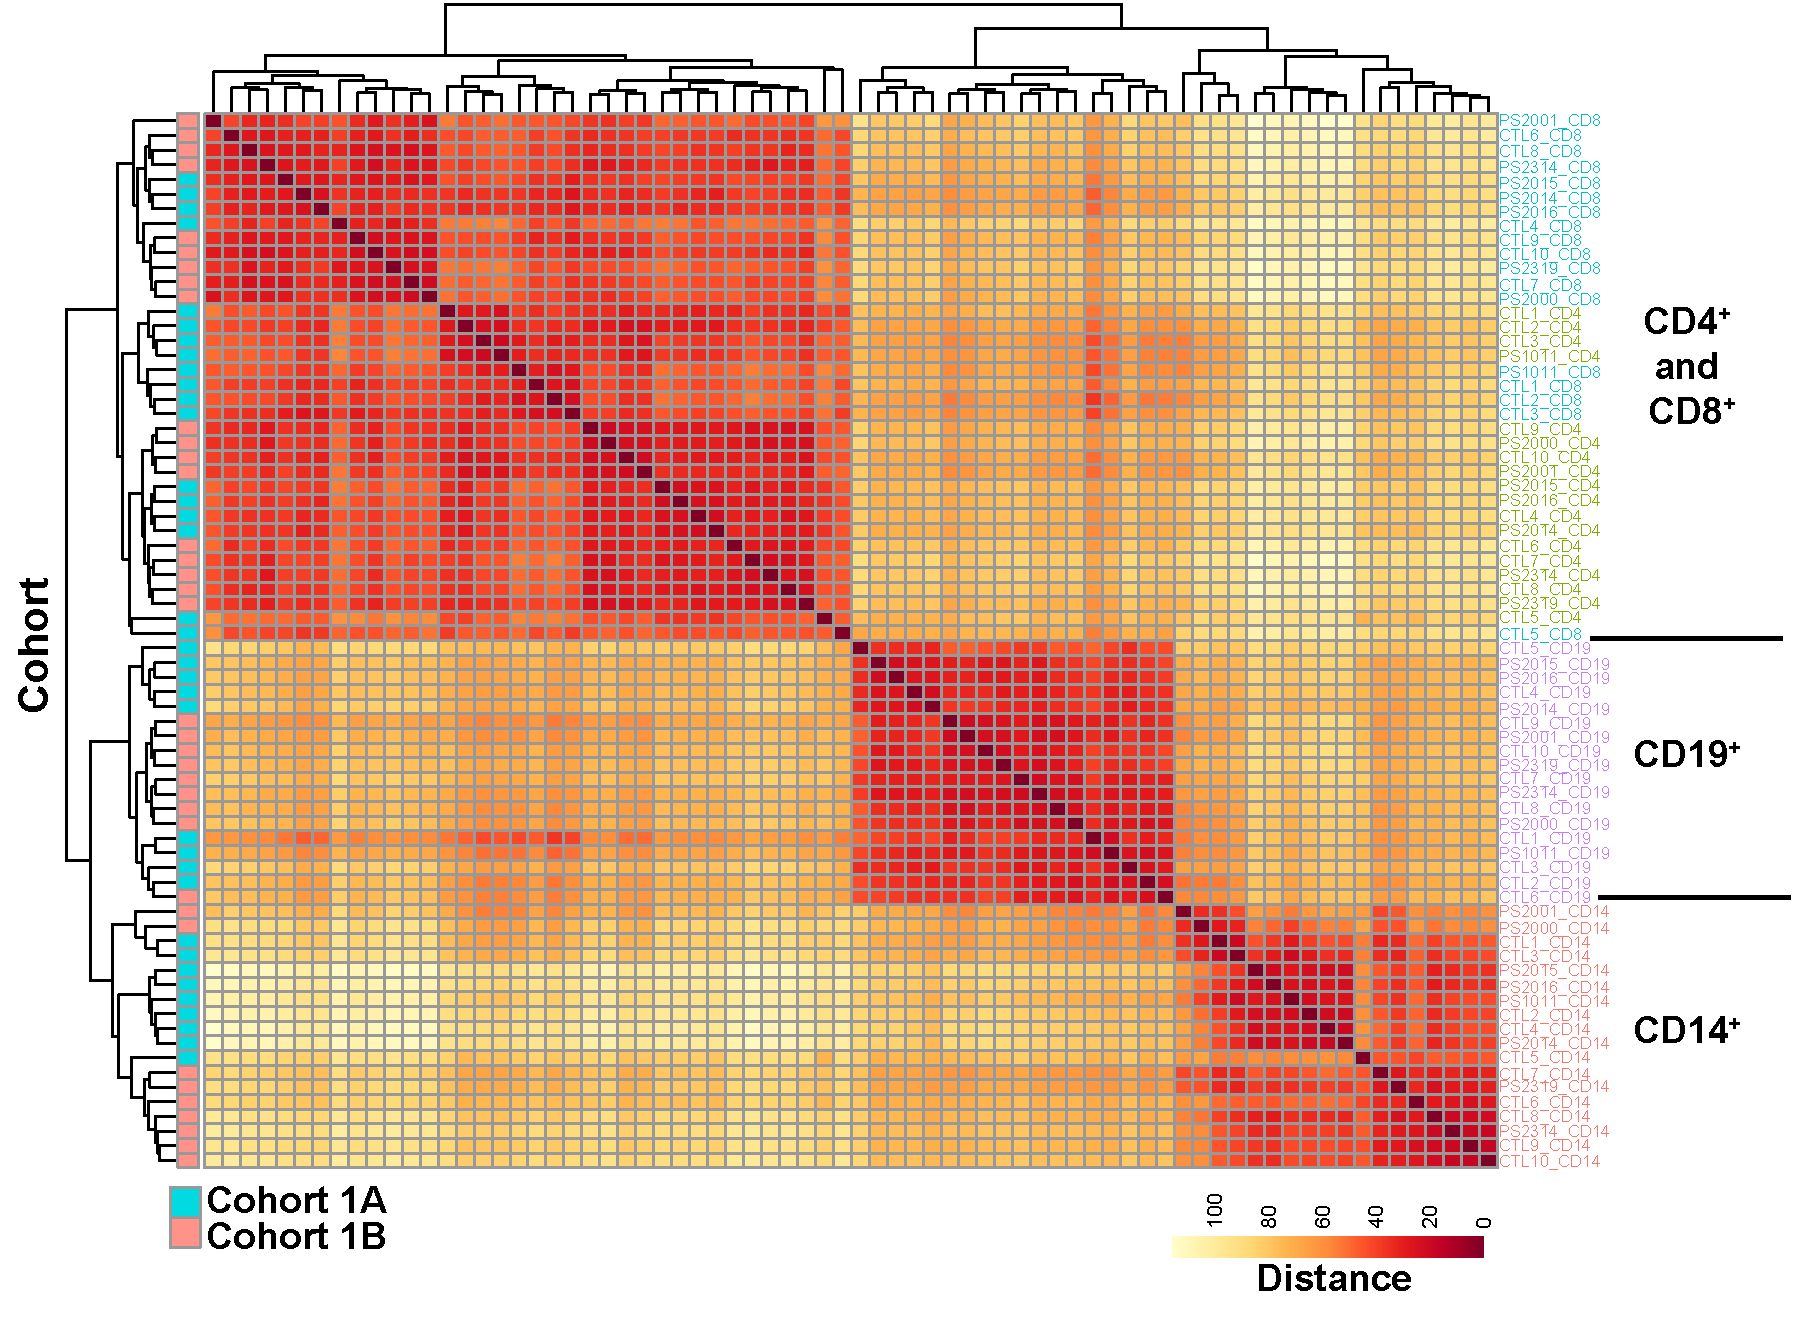
\includegraphics[width=\textwidth]{./Results2/pdfs/ATAC_all_cell_types_heatmap_with_batch_annotation}
\caption{}
\end{subfigure}
~
\begin{subfigure}[b]{0.6\textwidth} 
%the [b] prevents offset in subcaptions
\centering
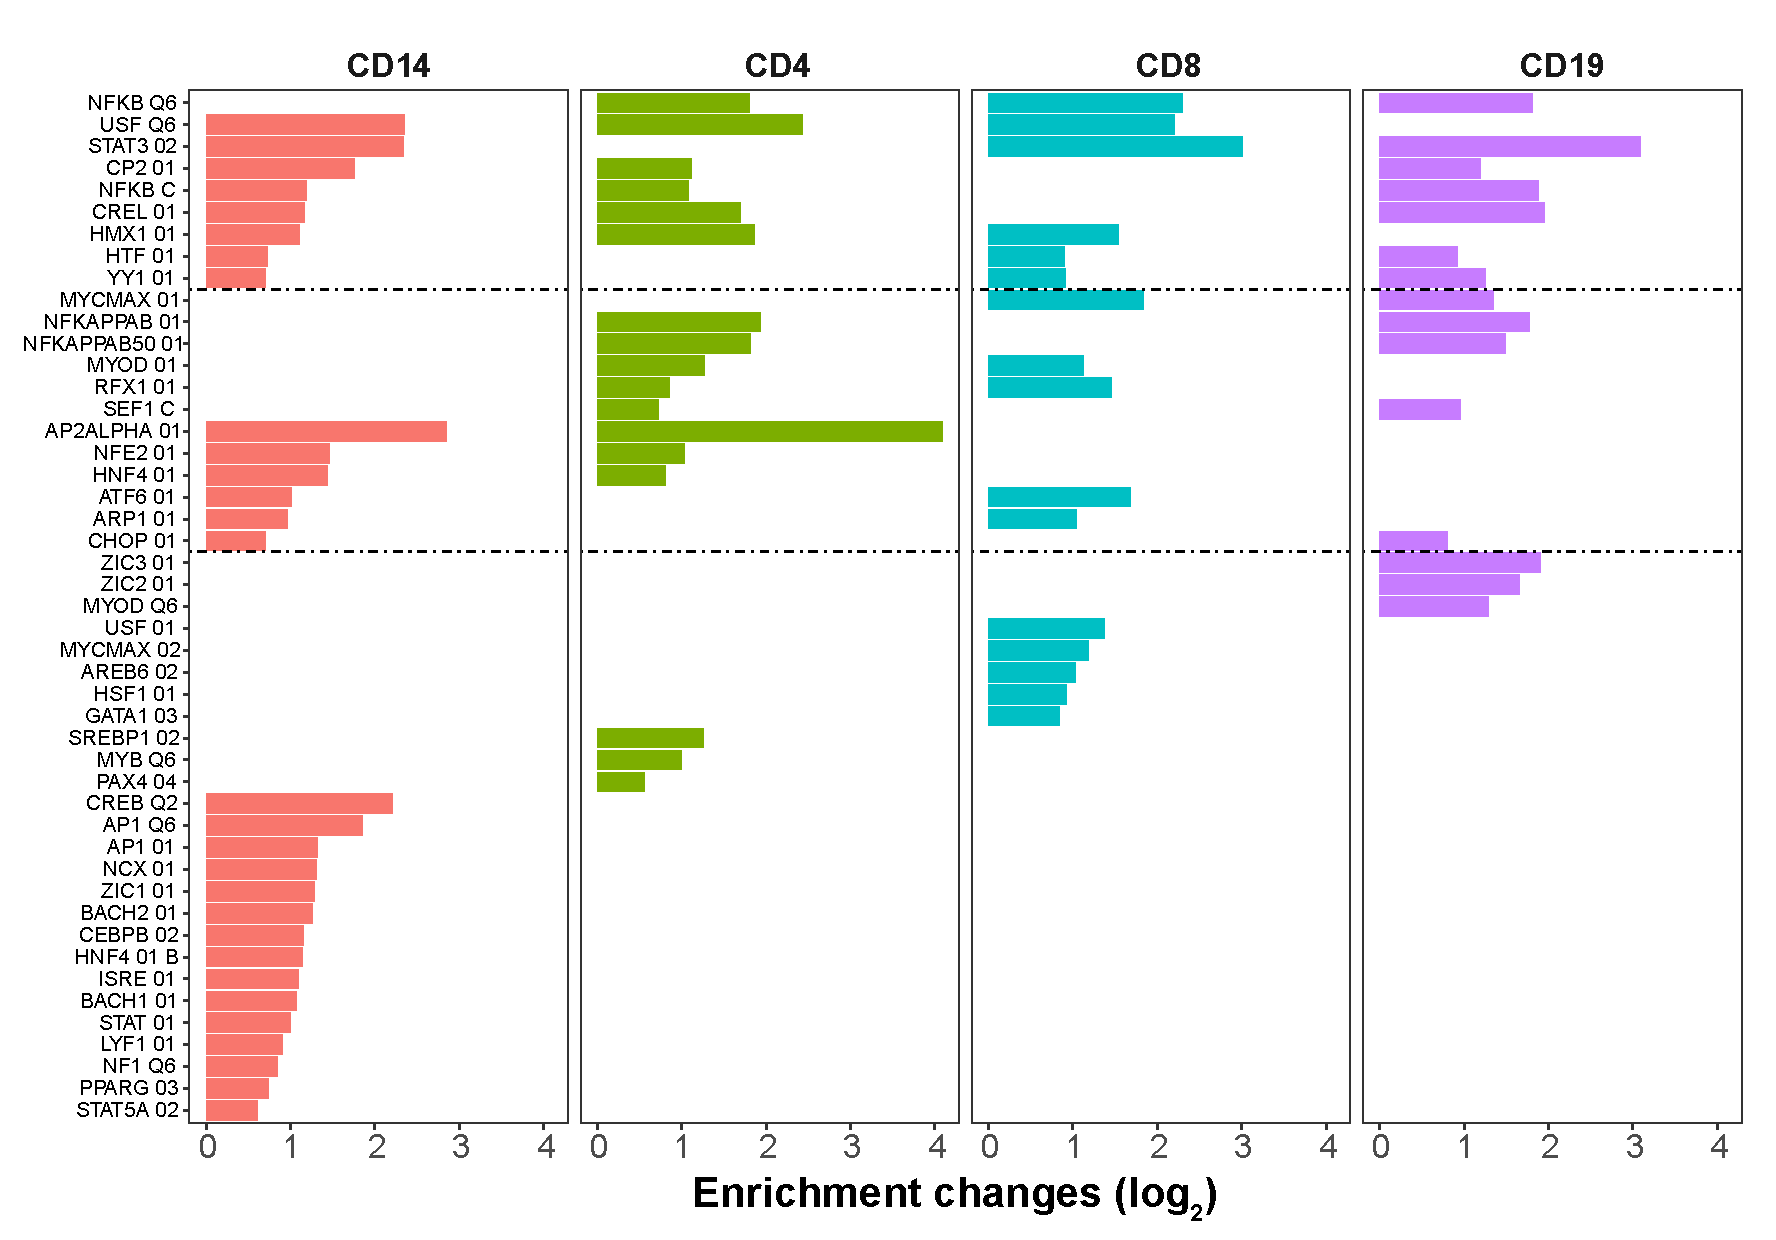
\includegraphics[width=\textwidth]{./Results2/pdfs/ATAC_PS_CTL_cell_type_specific_master_list_conserved_TFBS_enrichment}
\caption{}
\end{subfigure}
\caption[Clustered heatmap and conserved TFBS enrichment analysis in the consensus ATAC-seq regions identified in CD14$^+$ monocytes, CD4$^+$, CD8$^+$ and CD19$^+$ cells from the patients and controls cohort.]{\textbf{Clustered heatmap and conserved TFBS enrichment analysis in the consensus ATAC regions identified in CD14$^+$ monocytes, CD4$^+$, CD8$^+$ and CD19$^+$ cells from the patients and controls cohort.} a) Distance matrix and hierarchical clustering for the 72 samples was performed based on the normalised read counts retrieved for each sample at the regions included in a consensus master list of ATAC-seq enriched sites built across all four cell types (ML\_all). Clusters have been additionally annotated using cohort identity. b) Enrichment analysis for the conserved TFBS was performed for each of the ATAC-seq cell type master lists of regions used for downstream differential analysis. Enrichment was tested for 258 human conserved TFBS identified by Transfac using position-weight matrices based on experimental results in the scientific literature. Significant enrichment using FDR$<$0.01.}
\label{figure:ATAC_PS_CTL_heatmap_TFBS}
\end{figure}


Each of the four cell type master lists of ATAC-seq peaks (ML\_CD14, ML\_CD4, ML\_CD8, and ML\_CD19) used for the downstream differential chromatin accessibility analysis (explained in Chapter \ref{ch:Mat}), presented the highest percentage of regions annotated as gene promoters, intronic and intergenic, as expected for ATAC-seq (Figure \ref{figure:ATAC_PS_CTL_genomic_annotation}). \textit{cis}-eQTL SNPs from a number of immune cell types, including CD14$^+$ monocytes (unstimulated and stimulated), B cells, neutrophils, CD4$^+$ and CD8$^+$ cells \parencite{Fairfax2012, Fairfax2014, Kasela2016}, were enriched within the ATAC consensus peak list of each cell type. For example, eQTLs from unstimulated and stimulated (LPS or IFN-$\gamma$) monocytes were the most significantly enriched (FDR$<$0.01) in the ML\_CD14 (unstimulated fold-enrichment 5.1, LPS 2h fold-enrichment 4.7 and IFN-$\gamma$ fold-enrichment 5.0) when compared to the other eQTL datasets. Similarly, \textit{cis}-eQTLs from CD4$^+$ and CD8$^+$ were the most enriched datasets (fold-change 8.3 and 8, respectively) in the ML\_CD8. The specificity and functional relevance of each cell type master list was further reinforced by the significant enrichment (FDR$<$0.01) of conserved TFBS within those ATAC-seq regions (Figure \ref{figure:ATAC_PS_CTL_heatmap_TFBS} b). For example, enrichment of conserved NF$\kappa$B binding motifs(NFKB Q6, NFKB C and NFKAPPAB 01) was identified across the master lists from the different cell types. Conserved binding motifs for TF involved in T cell biology, such as AREB6 (ZEB1), ATF6 and the heat-shock transcription factor HSF1 \parencite{Guan2018,Yamazaki2009,Gandhapudi2013}, were enriched in the ML\_CD8. 
%For example, enrichment of conserved binding motifs for AREB6 (ZEB1) involved in CD8$^+$ T effector and memory cell fate \parencite{Guan2018}, ATF6 implicated in NF$\kappa$B activation \parencite{Yamazaki2009} and the heat-shock transcription factor HSF1 regulator of T cell division under different types of stress \parencite{Gandhapudi2013} was found in the ML-CD8. 
Overall, the enrichment of eQTL SNPs and conserved TFBS highlighted the potential of each cell type master list to harbour functional relevant differences in chromatin accessibility between psoriasis patients and controls.



\subsubsection{Differential chromatin accessibility analysis}

Differential chromatin accessibility analysis between patients and controls was performed on the ATAC-seq normalised read counts for the regions of each cell type master list using DESeq2. PCA analysis on these data prior to the differential analysis revealed a batch effect correlating with the different ATAC-seq protocols used in cohort 1A and cohort 1B (standard ATAC-seq and FAST-ATAC, respectively) (Figure \ref{figure:ATAC_RNAseq_batch_effect} a). Therefore, the ATAC-seq protocol was included as a covariate in the differential analysis model. Moreover, CTL5 appeared as a cohort 1A outlier for all the cell types (representative example Figure \ref{figure:ATAC_RNAseq_batch_effect} a) and was also removed from the differential analysis.

Genome-wide differential chromatin accessibility analysis revealed 55 significant (FDR$<$0.05) DARs between psoriasis patients and healthy controls in CD8$^+$ cells (Table \ref{tab:ATAC_PS_CTL_differential_analysis_results}), of which 17 showed FDR$<$0.01. Conversely, CD14$^+$ monocytes, CD4$^+$ and CD19$^+$ cells only presented one or no DARs. 

% RANKL in RA  https://onlinelibrary.wiley.com/doi/full/10.1002/art.21731
% RANKL PsA https://www.ncbi.nlm.nih.gov/pmc/articles/PMC153764/

\begin{table}[htbp]
%\setlength{\tabcolsep}{20pt} only to stretch the columns if you want
%\renewcommand{\arraystretch}{1.5}
\centering
\begin{tabular}{@{} c c}
\toprule
\textbf{Cell type}   & \textbf{Number of DARs} \\
                     & \textbf{FDR$<$0.05}     \\
\midrule
\midrule
CD14$^+$             & 1 \\                 
tCD4$^+$              & 0 \\
tCD8$^+$              & 55 \\
CD19$^+$             & 1 \\
\bottomrule 
\end{tabular}
\medskip %gap
\caption[Summary results from the differential chromatin accessibility analysis between psoriasis patients and healthy controls in CD14$^+$ monocytes, CD4$^+$, CD8$^+$ and CD19$^+$ cells.]{\textbf{Summary results from the differential chromatin accessibility analysis between psoriasis patients and healthy controls in CD14$^+$ monocytes, CD4$^+$, CD8$^+$ and CD19$^+$ cells.} The number of differentially accessible regions (DARs) refers to those statistically significant when using a cut-off for background reads of 80\% (see Chapter \ref{ch:Results1} and a FDR$<$0.05. No threshold for the FC was applied in this analysis.}
\label{tab:ATAC_PS_CTL_differential_analysis_results}
\end{table}
\bigskip %bigger space


Annotation of the 55 CD8$^+$ DARs using cell type specific Roadmap Epigenomics chromatin segmentation maps revealed the potential for some of the regions to be involved in regulation of gene expression, including 24 (44.4\%) weak enhancers, 7 (12.9\%) active promoters, 6 (11.1\%) weak promoter and 2 (3.7\%) strong enhancers. The functional relevance of the DARs in terms of regulation of gene expression was further investigated by integration of the CD8$^+$ cell eRNA data from the FANTOM5 project. Only 8 of the CD8$^+$ DARs overlapped significantly expressed eRNAs. These include a region at the TSS of the \textit{TNSF11} gene and another upstream the \textit{IL7R} promoter, which were more accessible in the psoriasis patients compared to the healthy controls (Figure \ref{figure:ATAC_PS_CTL_CD8_TNFSF11_IL7R_tracks} a and b). The two DARs also overlap chromatin harbouring H3K4me3, a histone mark indicating an active promoter, and H3K27ac consistent with the transcription of those regions as eRNAs in tCD8$^+$ cells according to FANTOM5.

\begin{figure}[htbp]
\centering
\begin{subfigure}{0.5\textwidth}
\centering
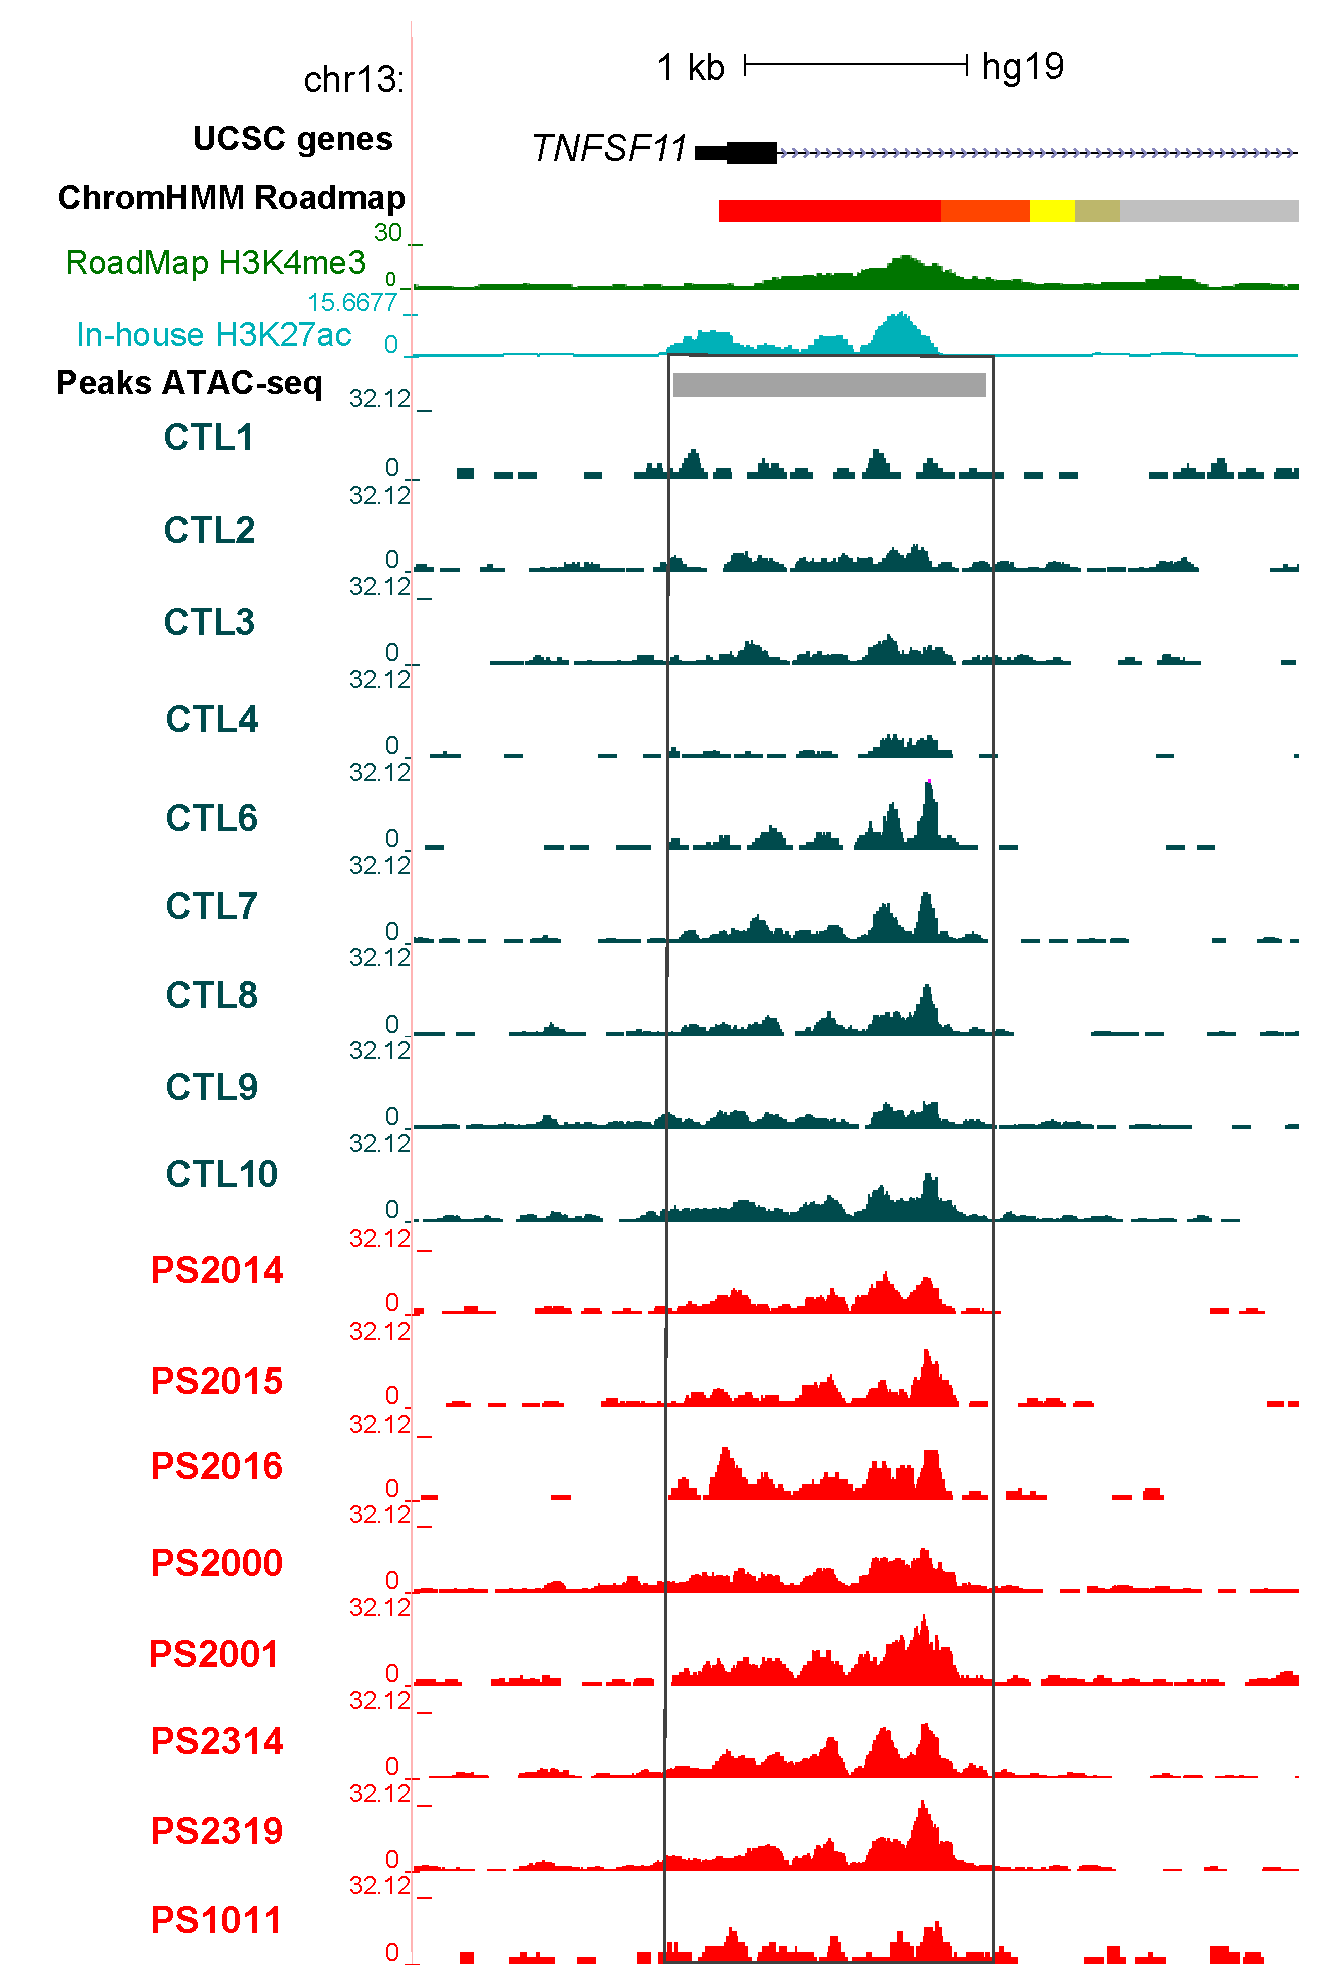
\includegraphics[width=\textwidth]{./Results2/pdfs/UCSC_ATAC_CD8_peak_prom_TNFSF11}
\caption{\textbf{}}
% The percentage sign indicated that the other subfig goes side by side
\end{subfigure}%
\begin{subfigure}{0.5\textwidth}
\centering
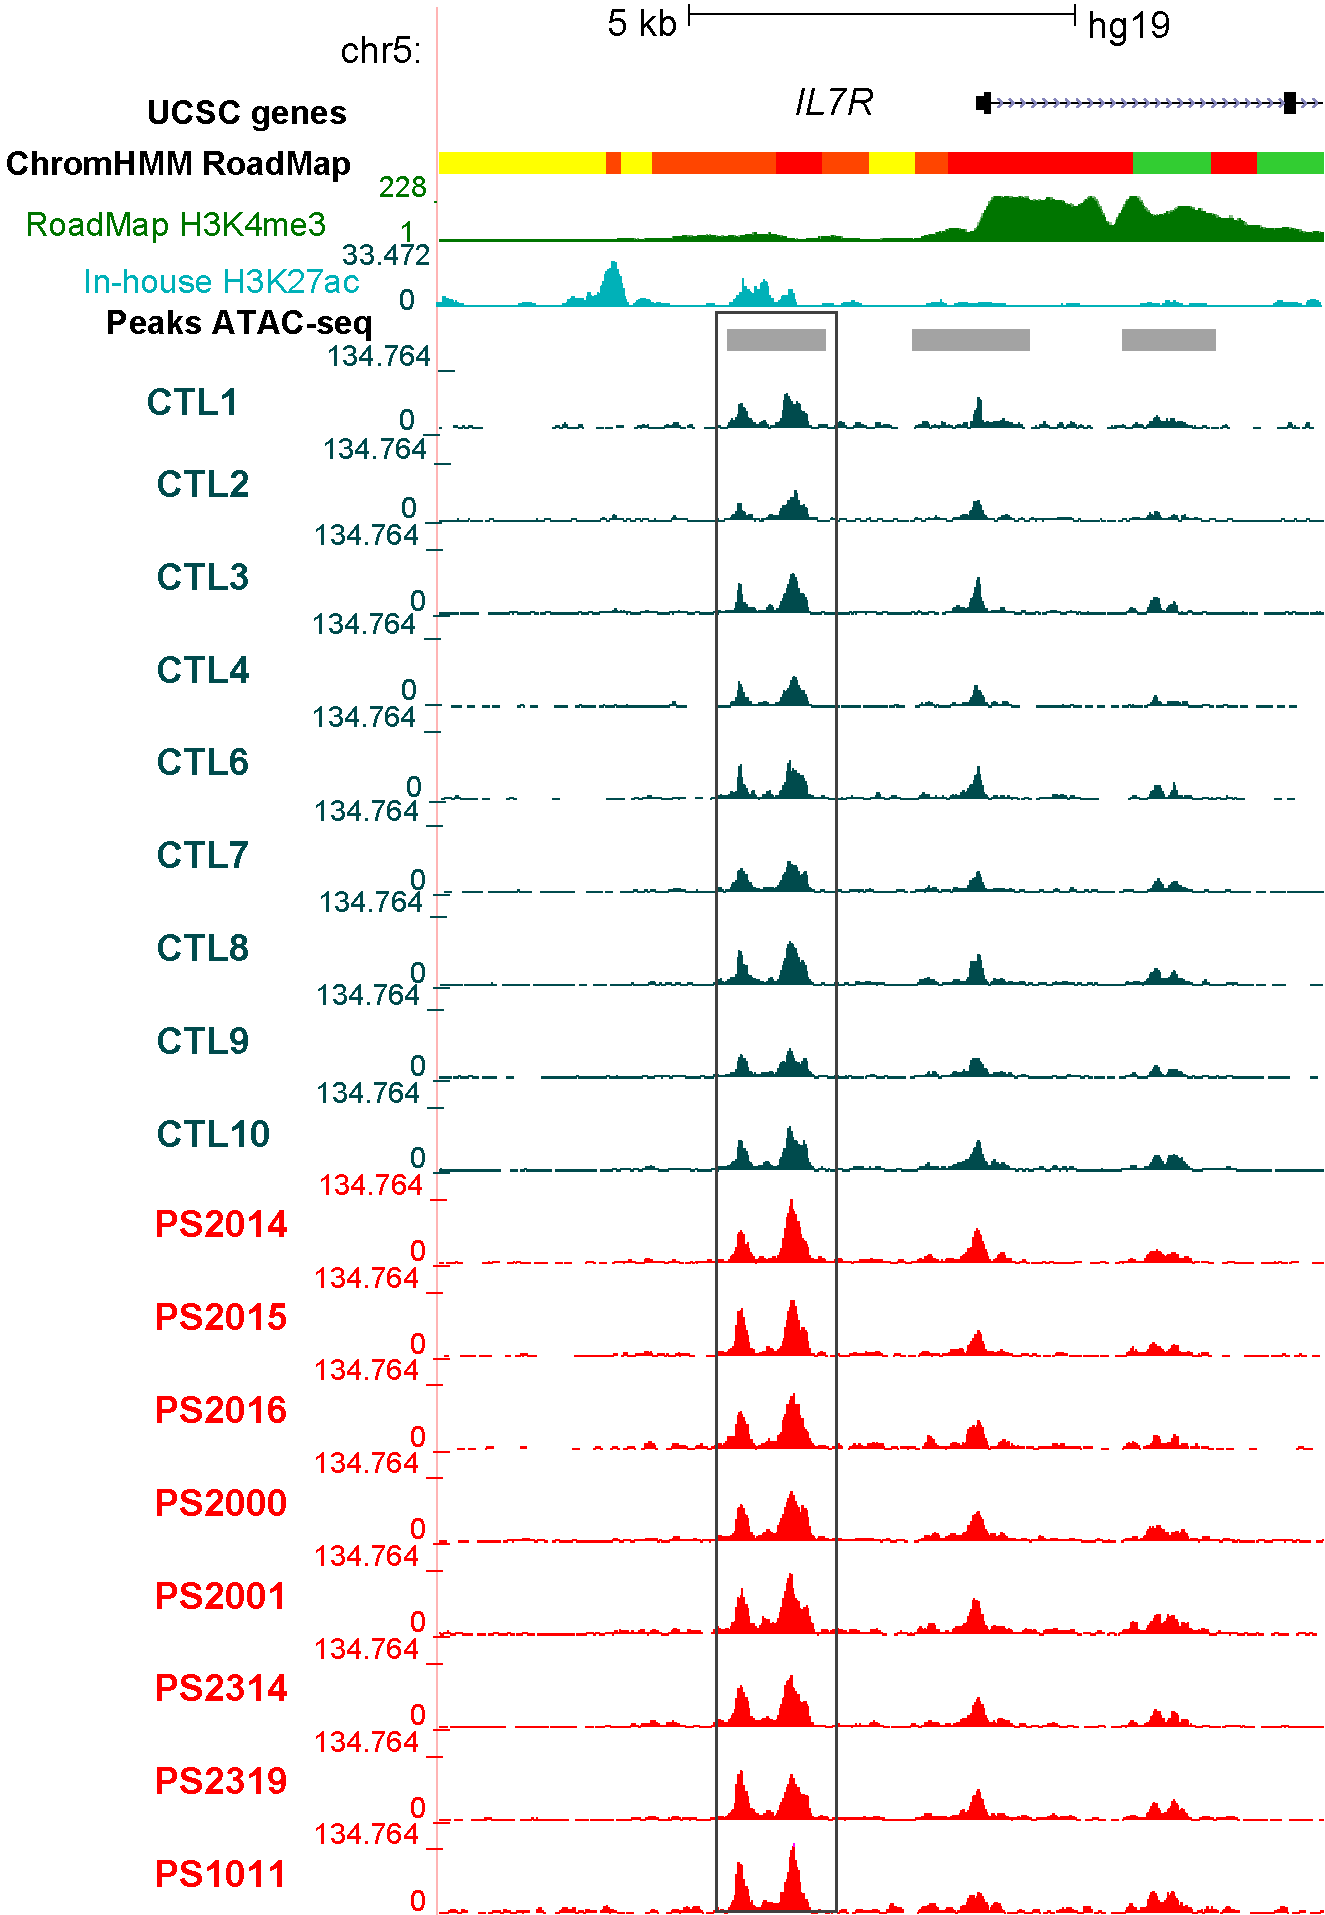
\includegraphics[width=\textwidth]{./Results2/pdfs/UCSC_ATAC_CD8_normalised_peak_enh_IL7R}
\caption{\textbf{}}
\end{subfigure}
\caption[Epigenetic landscape at two ATAC differential accessible regions between patients and controls in CD8$^+$ cells.]{\textbf{Epigenetic landscape at two ATAC differential accessible regions between patients and controls in CD8$^+$ cells.} UCSC Genome Browser view illustrating the normalised ATAC read density (y-axis) in DARs located at a) the promoter of \textit{TNFSF11} gene and b) up-stream the \textit{IL7R} gene (x-axis). Both DARs were more open in tCD8$^+$ cells from psoriasis compared to controls. Tracks are colour-coded by condition: control(CTL)=dark turquoise and psoriasis (PS)=red. The Epigenome Roadmap chromatin segmentation map and H3K4me3 for tCD8$^+$ cells are also shown, together with a representative track from the in-house ChIPm H3K27ac in this cell type. All DARs were significant based on FDR$<$0.05 and no FC cut-off.}
\label{figure:ATAC_PS_CTL_CD8_TNFSF11_IL7R_tracks}
\end{figure} 



%Both of them are relevant genes in driving and maintaining the inflammatory response. For example, \textit{TNFSF11} is a cytokine from the TNF family involved in the regulation of T cell-dependent immune response and osteoclast differentiation in RA and PsA \parencite{Miranda‐Car\'ús2006,Ritchlin2003}. \textit{TNFSF11} is also downstream the lead SNPs for a CD risk locus \parencite{ImmunoBase}. Interestingly, the \textit{TNFSF11} protein, RANKL was found to be overexpressed in epidermis from psoriasis patients compared to controls and cutaneous lupus erythematosus, highlighting the role of this gene in the pathophysiology of psoriasis \parencite{Toberer2011}. On the other hand \textit{IL7R} is a proximal gene to SLE and MS, amongst others, and the axis IL-7/IL-7R has been found to drive IL7 indepdendent TNF-$\alpha$ inflammation in RA patients presenting iTNF resistence \parencite{van Roon2017}. 
Other potentially interesting CD8$^+$ DARs were found nearby genes such as the MAPK \textit{MAP3K7CL} and \textit{NFKB1}; However they were not at regions annotated as enhancers or overlaped with experimentally validated eRNAs. 

%Additionally, none of the CD8$^+$ DARs were found within an LD block (r$^2$$\geq$0.8) of the psoriasis risk GWAS loci.

\subsubsection{Integration of H3K27ac ChIPm and ATAC-seq chromatin accessibility profiles}

Although a very low number of differentially H3K27ac modified and DARs were found between psoriasis and control samples in the four cell types , commonalities in the disease specific changes were investigated. The the H3K27ac ChIPm and ATAC differential sites between psoriasis and control individuals only showed one overlapping region in CD8$^+$ cells. The DARs and differentially H3K27ac site was located within an intron of the D-tyrosyl-tRNA deacylase 1 (\textit{DTD1}) gene (Figure \ref{figure:ATAC_ChIPm_overlap_DTD1_region_track}). This region presented lower levels of H3K27ac (4 patients versus 4 controls) and was less accessible (8 patients versus 9 controls) in the psoriasis patients when compared to healthy controls (Figure). This differential region was annotated as an active enhancer according to the tCD8$^+$ ChromHMM segmentation map and did not interact with the promoter of any gene according to Hi-C and promoter Hi-C data in tCD8$^+$ cells \parencite{Javierre2016}. Conversely, SNPs within this region were eQTL for \textit{DTD1} in whole blood (https://gtexportal.org/home/eqtls). 

%This gene has been described to play a role in the initiation of DNA replication and has been associated with aspirine-intolerance in asthmatics \parencite{Pasaje2011}. However, no studies have yet highlighted a direct link of this gene with the pathophysiology of chronic inflammatory diseases.  

\begin{figure}[htbp]
\centering
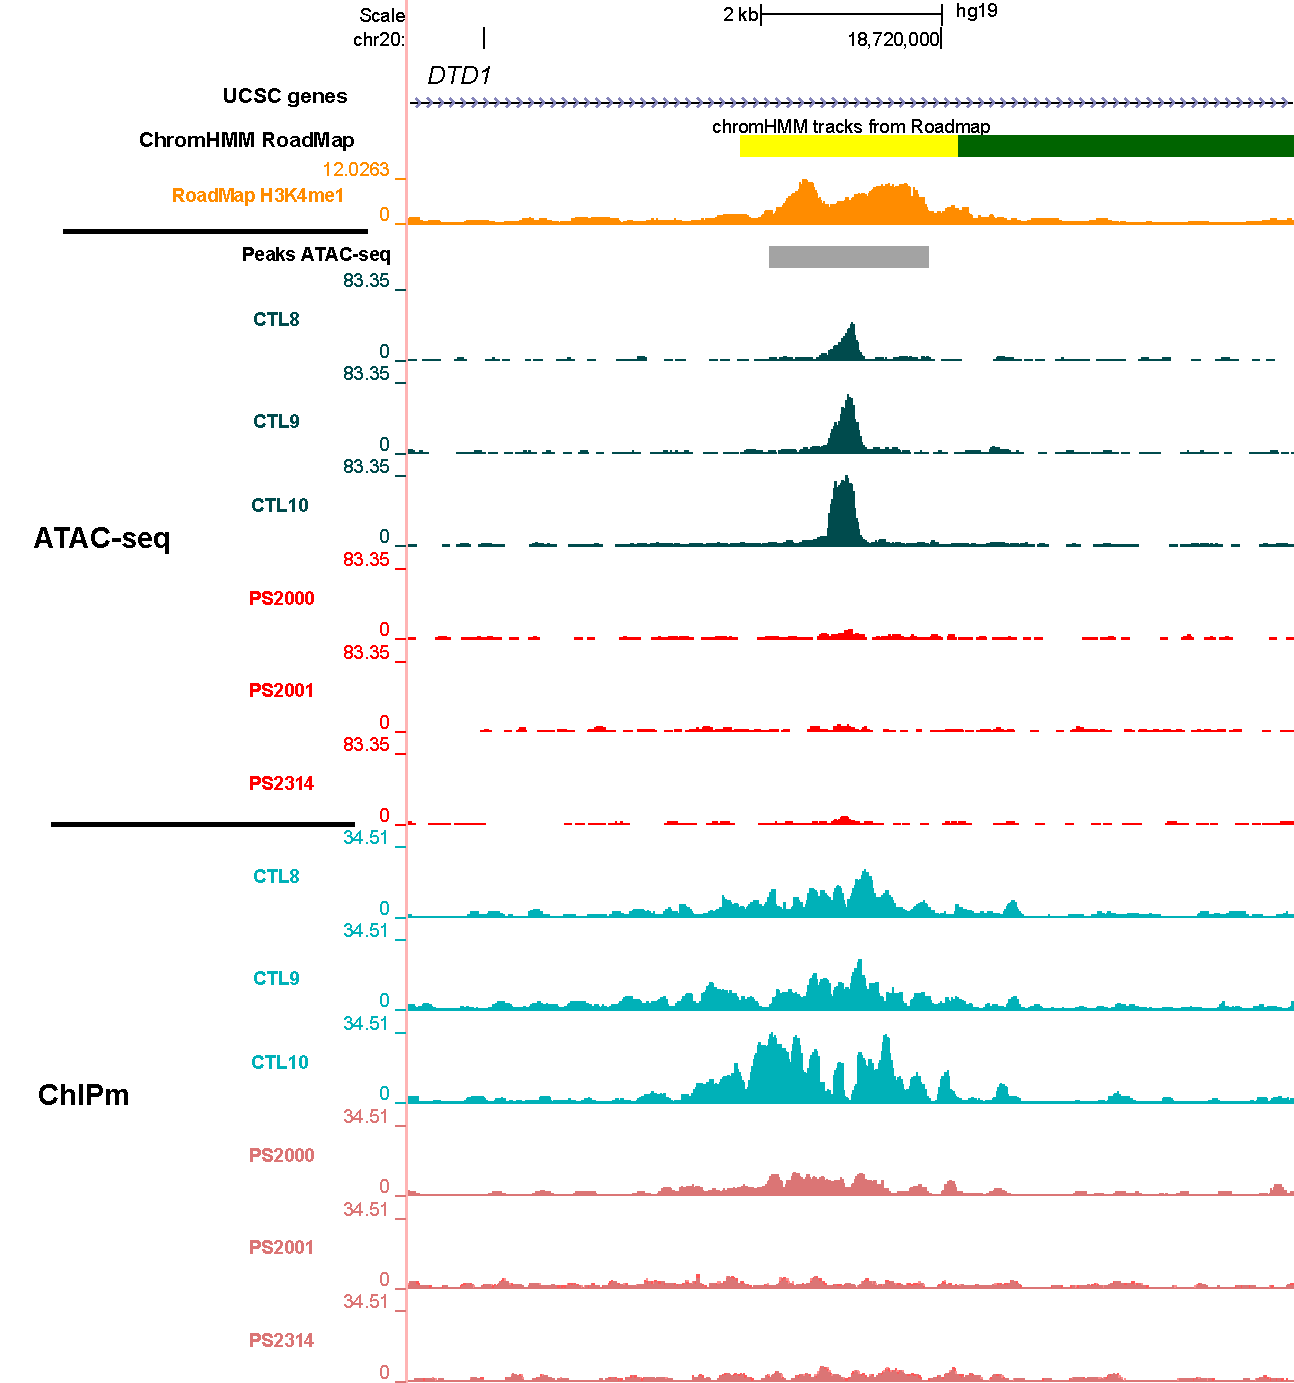
\includegraphics[width=0.6\textwidth]{./Results2/pdfs/ChIPm_H3K27ac_UCSC_CD8_DTD1_track}
\caption[Epigenetic landscape at the only overlapping region identified as differentially accessible and differentially H3K27ac modified between psoriasis patients and controls.]{\textbf{Epigenetic landscape at the only overlapping region identified as DARs and differentially H3K27ac modified between psoriasis patients and controls.} UCSC Genome Browser view illustrating the normalised ATAC read density and H3K27ac normalised fold-enrichment (y-axis) at an intron of the \textit{DTD1} gene (x-axis) in tCD8$^+$ cells. This region was identified as less accessible and less enriched for H3K27ac modifications in psoriasis patients compared to healthy controls. Tracks are colour-coded by condition and assay: control(CTL)=dark and light turquoise and psoriasis (PS)=light and dark red, for ATAC and ChIPm respectively. The Epigenome Roadmap chromatin segmentation map and H3K4me1 for tCD8$^+$ cells are also shown.}
\label{figure:ATAC_ChIPm_overlap_DTD1_region_track}
\end{figure}




\subsection{Gene expression analysis in psoriasis circulating immune cells}



\subsubsection{Data processing and quality control}

In addition to characterising the chromatin accessibility landscape, gene expression profiles in psoriasis and healthy individuals were also analysed for the same four primary circulating immune cell types using RNA-seq. The percentage of RNA-seq reads mapping to a unique location in the genome using STAR (see Chapter \ref{ch:Mat}) was appropriate (minimum recommended 70 to 80\%), ranging between 79.64 and 86.19\% across the 72 samples (Figure \ref{figure:RNAseq_mapping_rate_and_reads_in_genes} a). After appropriate filtering, all the samples had at least 20 million reads (as required by ENCODE standards) mapping to a comprehensive list of Ensembl features, including protein coding genes and lncRNAs (Figure \ref{figure:RNAseq_mapping_rate_and_reads_in_genes} b). The median total reads mapping to Ensembl features was greater for CD14$^+$ monocytes when compared to the other three cell types. Interestingly, in all four cell types analysed, greater mapping rates and total reads mapping to Ensembl features were observed for cohort 1B samples when compared to cohort 1A. These differences were attributed to the library preparation and sequencing of each cohort in two different batches.  

\begin{figure}[htbp]
\centering
\begin{subfigure}{0.5\textwidth}
\centering
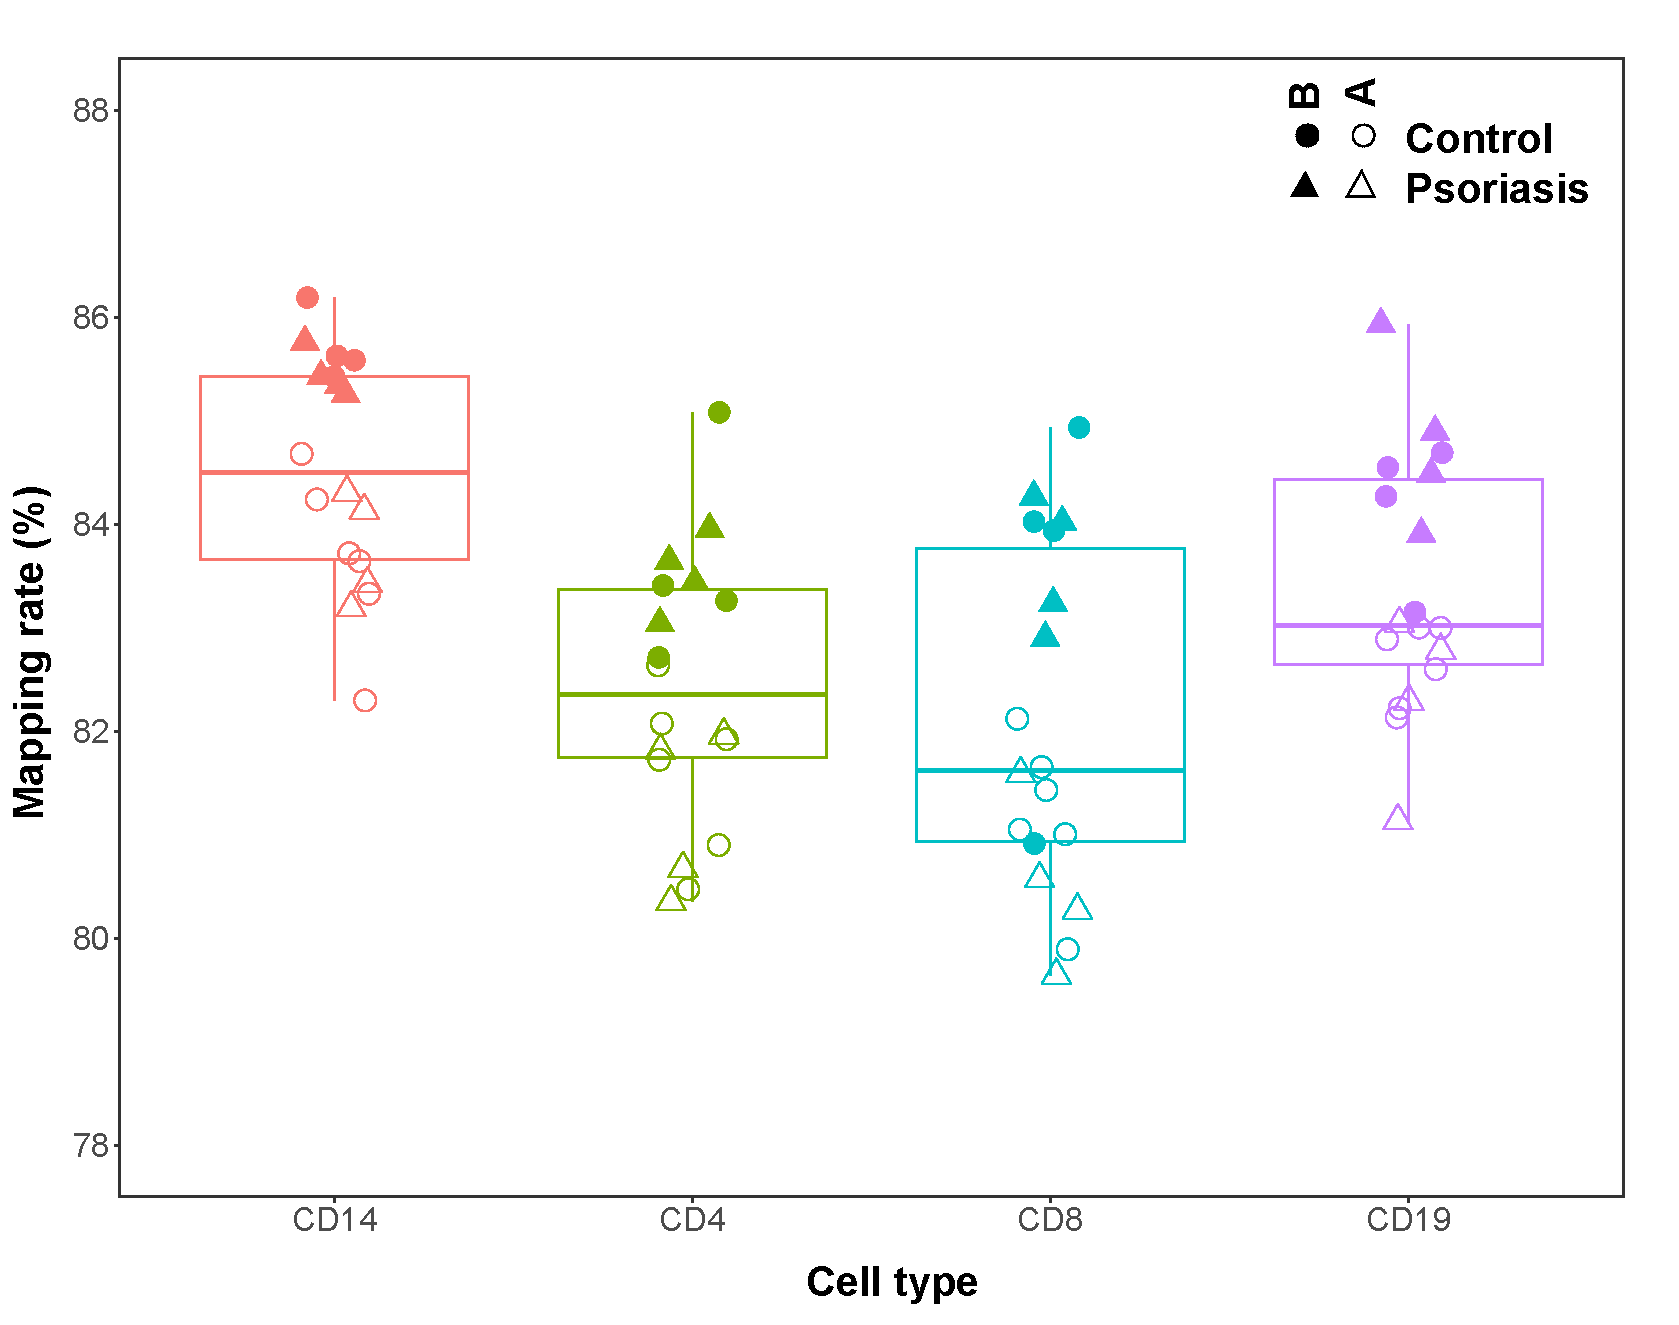
\includegraphics[width=\textwidth]{./Results2/pdfs/PS_CTL_RNAseq_uniquely_mapped_reads_rate_cell_type_batch_and_condition_boxplots}
\caption{\textbf{}}
% The percentage sign indicated that the other subfig goes side by side
\end{subfigure}%
\begin{subfigure}{0.5\textwidth}
\centering
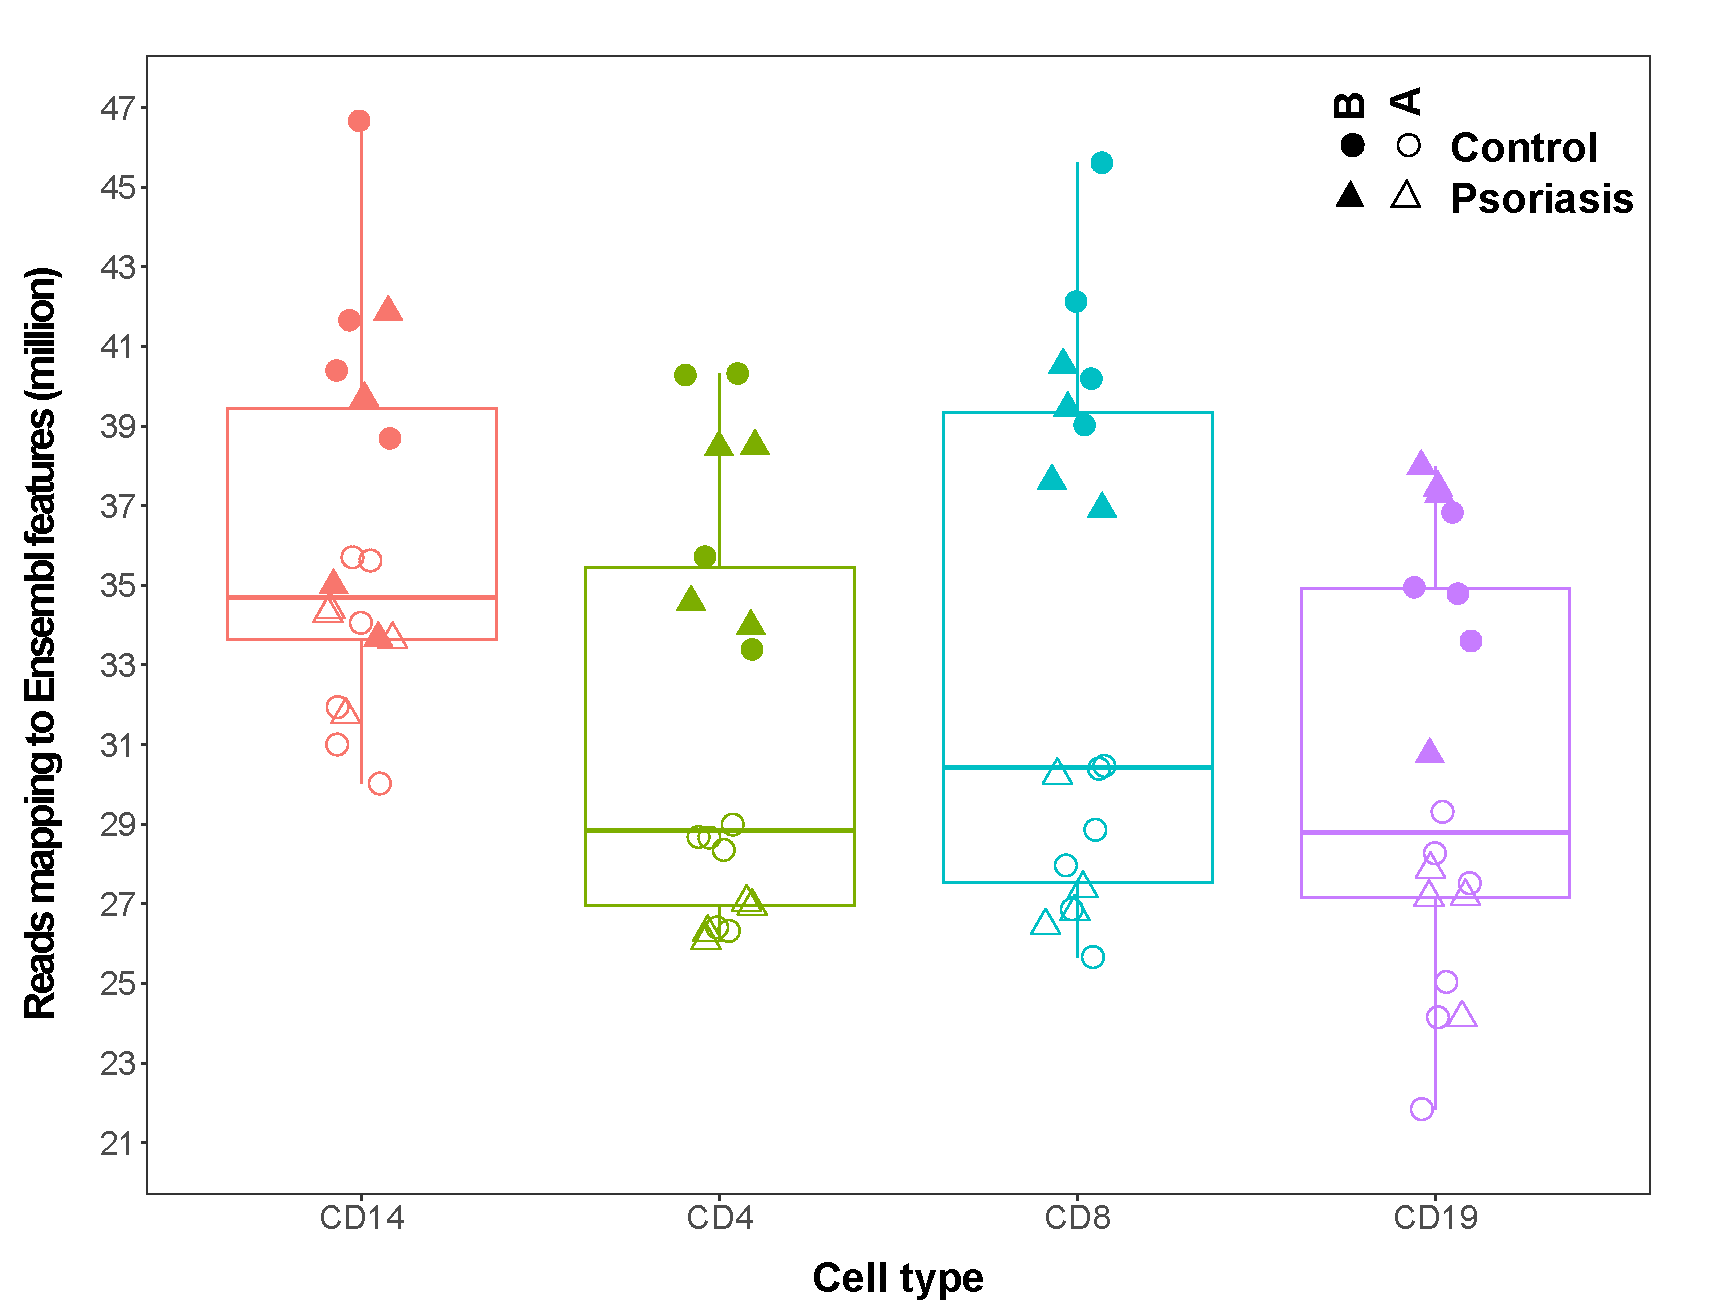
\includegraphics[width=\textwidth]{./Results2/pdfs/PS_CTL_RNAseq_total_reads_per_batch_cell_type_and_condition}
\caption{\textbf{}}
\end{subfigure}
\caption[Mapping rate and total reads after filtering (million) mapping to Ensembl genes in all the RNA-seq samples from psoriasis patients and controls in four cell types.]{\textbf{Mapping rate and total reads after filtering (million) mapping to Ensembl genes in all the RNA-seq samples from psoriasis patients and controls in four cell types.} a) The mapping rate refers to the percentage of total sequenced reads from each sample that uniquely mapped to a particular site of the genome. b) The total number of reads after filtering for non-uniquely mapped and duplicated reads that mapped to Ensembl features, including coding protein genes and lncRNAs.}
\label{figure:RNAseq_mapping_rate_and_reads_in_genes}
\end{figure} 


Similarly to ChIPm and ATAC-seq, the first and second PC from PCA analysis using the normalised number of reads mapping to each of the 20,493 Ensembl genes passing quality control (see Chapter \ref{ch:Mat}) showed that most variability was driven by cell type differences (Figure \ref{figure:RNAseq_PCA_and_heat_map} a). A heatmap illustrating sample distance based on the expression profile of each sample followed by hierarchical clustering revealed three main clusters corresponding to CD14$^+$ monocytes, CD4$^+$ and CD8$^+$ lymphocytes, and CD19$^+$ cells (Figure \ref{figure:RNAseq_PCA_and_heat_map} a). Within each cell type cluster, samples were further grouped by cohort (1A and 1B) and not by condition (psoriasis and control), consistent with the differences in mapping rate and total reads mapping to Ensembl genes observed across the two cohorts (Figure \ref{figure:RNAseq_mapping_rate_and_reads_in_genes} a and b). Clear correlation of sample batch with PC4 from the PCA analysis led to a very clear separation of the samples into cohort 1A and 1B, explaining 3\% of the total variance (Figure \ref{figure:ATAC_RNAseq_batch_effect} b). Consequently, batch was included in the DGE model as a covariate.  

\begin{figure}[htbp]
\centering
\begin{subfigure}{0.5\textwidth}
\centering
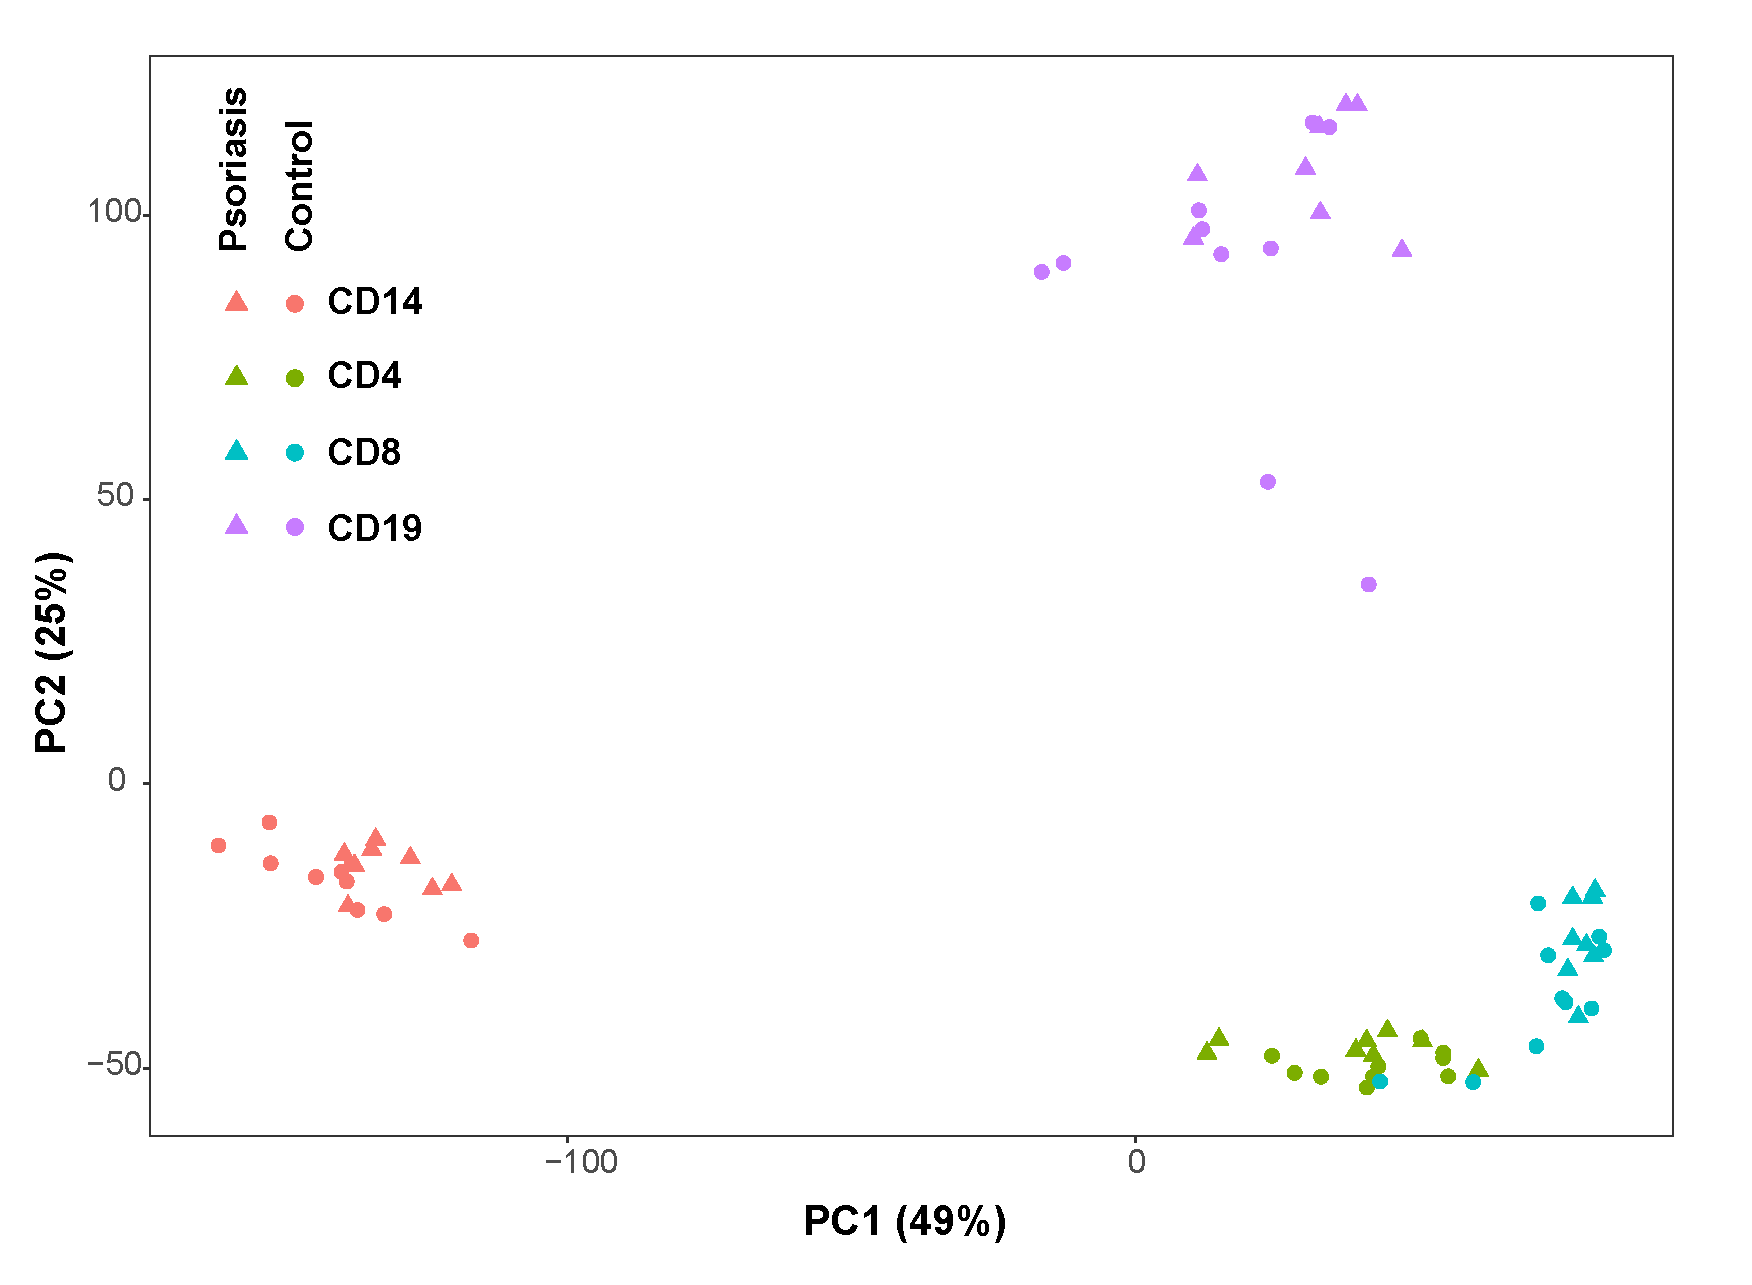
\includegraphics[width=\textwidth]{./Results2/pdfs/PS_CTL_all_samples_varied_PCA1and2_plot}
\caption{\textbf{}}
% The percentage sign indicated that the other subfig goes side by side
\end{subfigure}
\begin{subfigure}{0.5\textwidth}
\centering
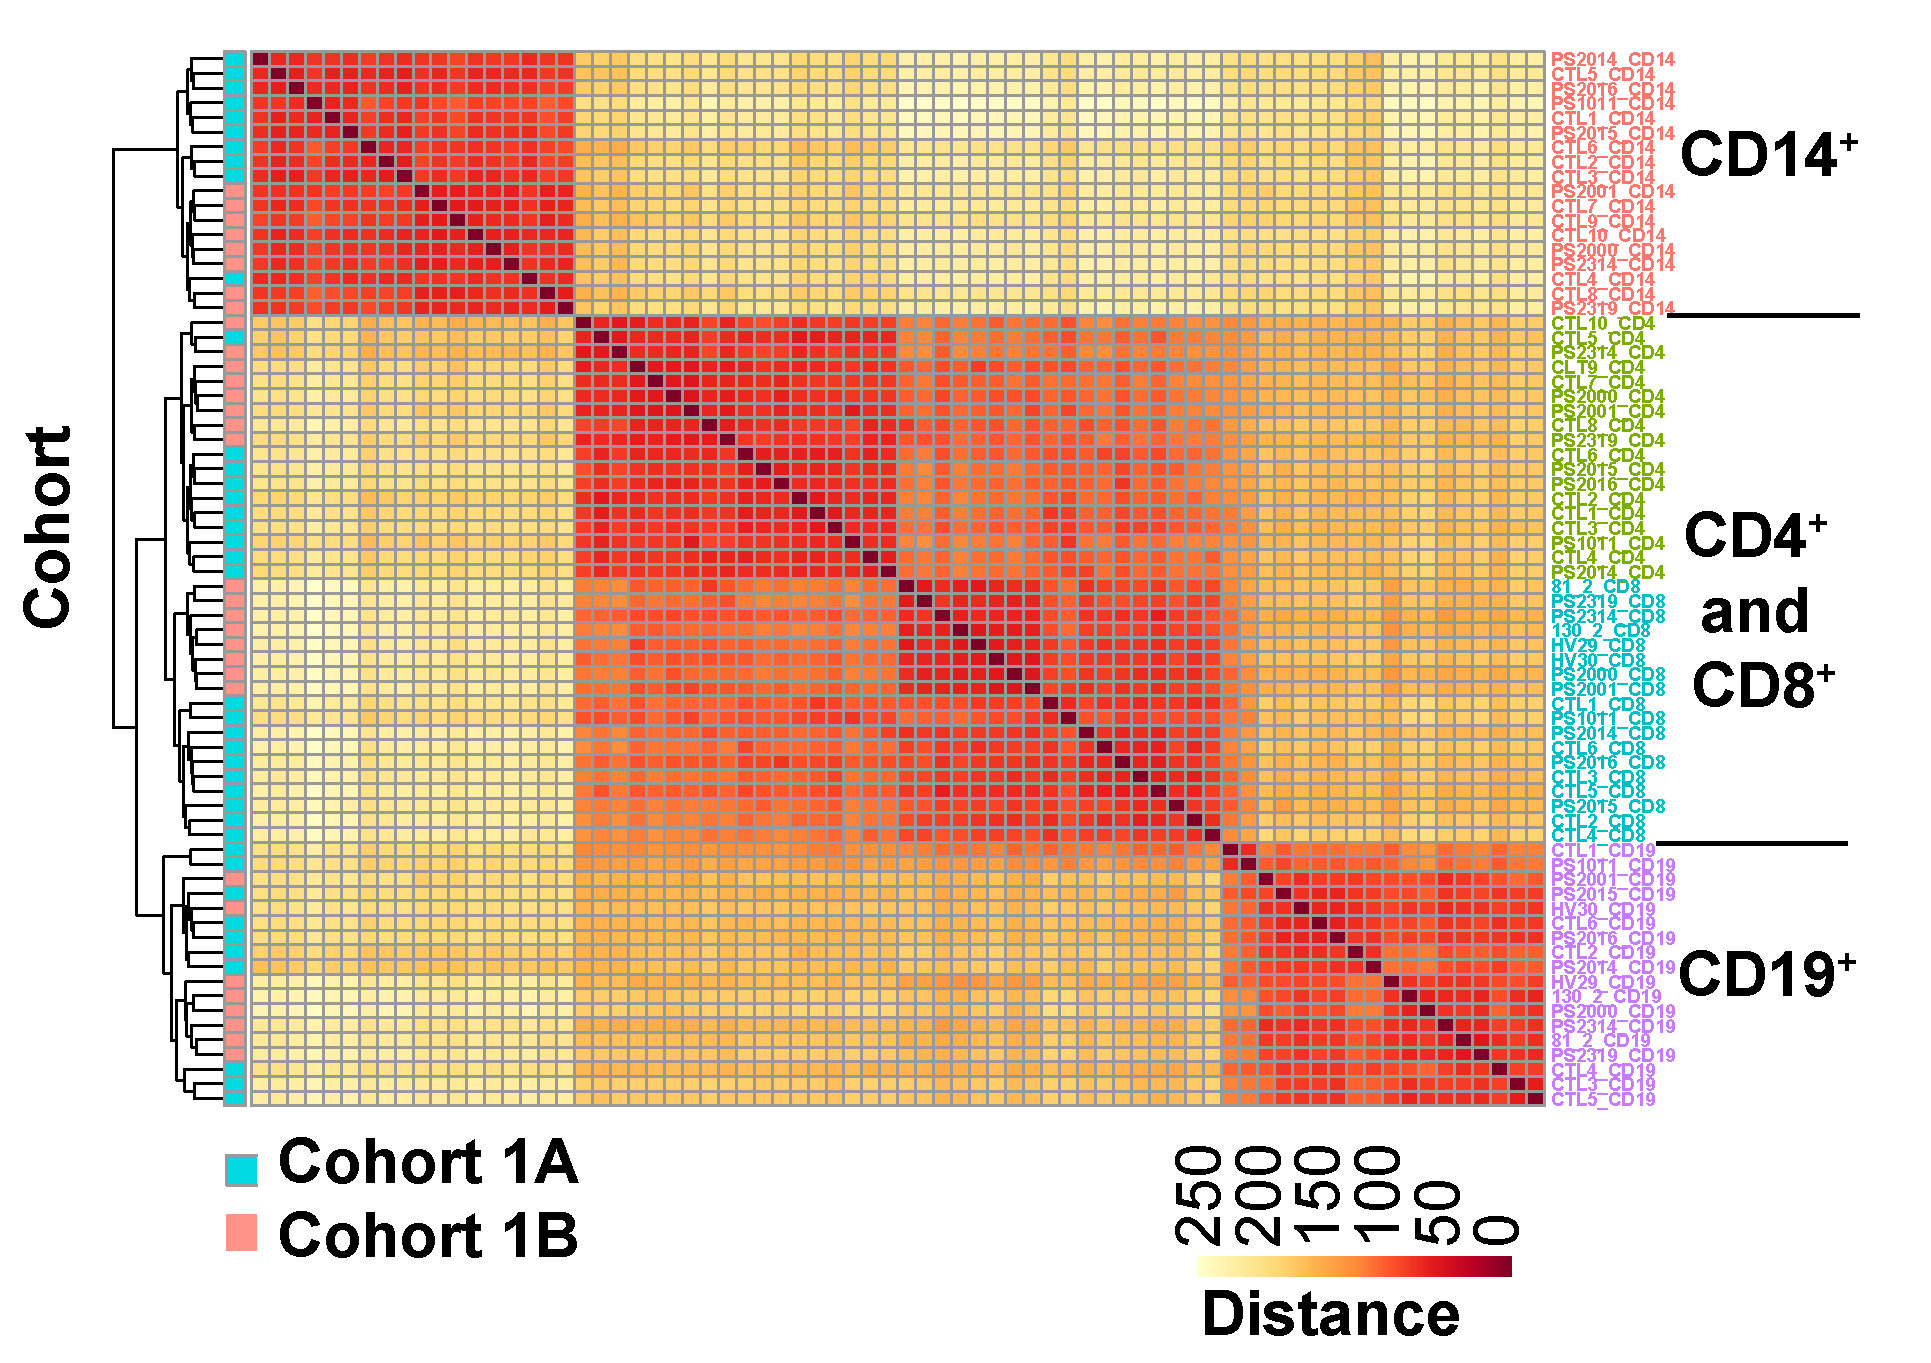
\includegraphics[width=\textwidth]{./Results2/pdfs/PS_CTL_all_samples_heatmap_including_batch}
\caption{\textbf{}}
\end{subfigure}
\caption[PCA analysis and sample distance heatmap with hierarchical clustering illustrating the sample variability based on the gene expression profiles.]{\textbf{PCA analysis and sample distance heatmap with hierarchical clustering illustrating the sample variability based on the gene expression profiles.} a) The first and second PCs (x-axis and y-axis, respectively) for the analysis using all the detected genes are represented to identify the main sources of variability across the 72 samples. Each point represents a sample, where the colour codes for cell type and the shape for condition. The proportion of variation explained by each principal component is indicated.b) Distance matrix clustering for the 72 samples was performed based on the normalised read counts mapping to 20,493 Ensembl featured remaining after appropriate filtering. Annotation of the clustering using cohort identity is included.}
\label{figure:RNAseq_PCA_and_heat_map}
\end{figure}


\subsubsection{mRNA and lncRNA differential expression}

DGE analysis between 8 psoriasis patients and 10 healthy controls in CD14$^+$ monocytes, tCD4$^+$, tCD8$^+$ and CD19$^+$ was performed using DESeq2 and including the cohort identity as a covariate to account for the batch effect previously mentioned. For each of the cell types a number of mRNAs were identified as differentially expressed at an FDR $<$0.05 or 0.01 (Table \ref{tab:RNAseq_PS_CTL_differential_analysis_results}).  

\begin{table}[htbp]
%\setlength{\tabcolsep}{20pt} only to stretch the columns if you want
%\renewcommand{\arraystretch}{1.5}
\centering
\begin{tabular}{@{} c c c}
\toprule
\textbf{Cell type}   & \textbf{mRNA}            & \textbf{lncRNA}           \\
                     & \textbf{FDR$<$0.05/0.01} & \textbf{FDR$<$0.05/0.01}  \\
\midrule
\midrule
CD14$^+$             & 671/229 & 28/8 \\               
tCD4$^+$              & 108/40  & 12/4 \\
tCD8$^+$              & 656/175 & 31/5 \\
CD19$^+$             & 167/71  & 6/2\\
\bottomrule 
\end{tabular}
\medskip %gap
\caption[Summary results from the DGE analysis between psoriasis patients and healthy controls in CD14$^+$ monocytes, CD4$^+$, CD8$^+$ and CD19$^+$ cells.]{\textbf{Summary results from the DGE analysis between psoriasis patients and healthy controls in CD14$^+$ monocytes, CD4$^+$, CD8$^+$ and CD19$^+$ cells.} The number of statistically differentially expressed mRNAs and lncRNAs are listed for two FDR threshold (FDR$<$0.05 and FDR$<$0.01). No threshold for the FC was applied in this analysis. The number and name of the lncRNAs overlapping with the Dolcino \textit{et al.}, 2018 study comparing PBMCs between PsA patients and healthy controls are also included. ($^{\ast}$) indicates dysregulation in the opposite direction between this data and Dolcino \textit{et al.}.}
\label{tab:RNAseq_PS_CTL_differential_analysis_results}
\end{table}
\bigskip %bigger spac

CD14$^+$ monocytes and tCD8$^+$ were the two cell types presenting the largest number of mRNAs with modulated expression between psoriasis patients and controls. %The more dysregulated gene expression response between patients and controls found in circulating psoriasis CD8$^+$ when compared to the CD4$^+$ may suggest the same hypothesis as in skin, where CD8$^+$ are considered the main effector cells undergoing activation upon the inflammatory stimuli \parencite(Nickoloff1999). Interestingly, CD19$^+$ presented a greater number of differentially expressed mRNAs than CD4$^+$. %regardless of their not yet having been implicated in disease (confirm).

The magnitude of the FC of gene expression between psoriasis patients and controls was moderate in all four cell types, with the largest changes in CD14$+$ monocytes and CD8$^+$ cells. Regarding the directionality of the statistically significant modulated genes (mRNa and lncRNAs) using FDR$<$0.05, CD14$^+$ monocytes (up 344, down 379) and CD4$^+$ (up 57, down 66) presented similar numbers of genes up-regulated and down-regulated in psoriasis patients when compared to the healthy controls. In contrast, in CD8$^+$ (up 278, down 429) and CD19$^+$ (up 29, down 148) a larger number of modulated genes were down-regulated in patients compared to controls.



\begin{figure}[htbp]
\centering
\begin{subfigure}{0.5\textwidth}
\centering
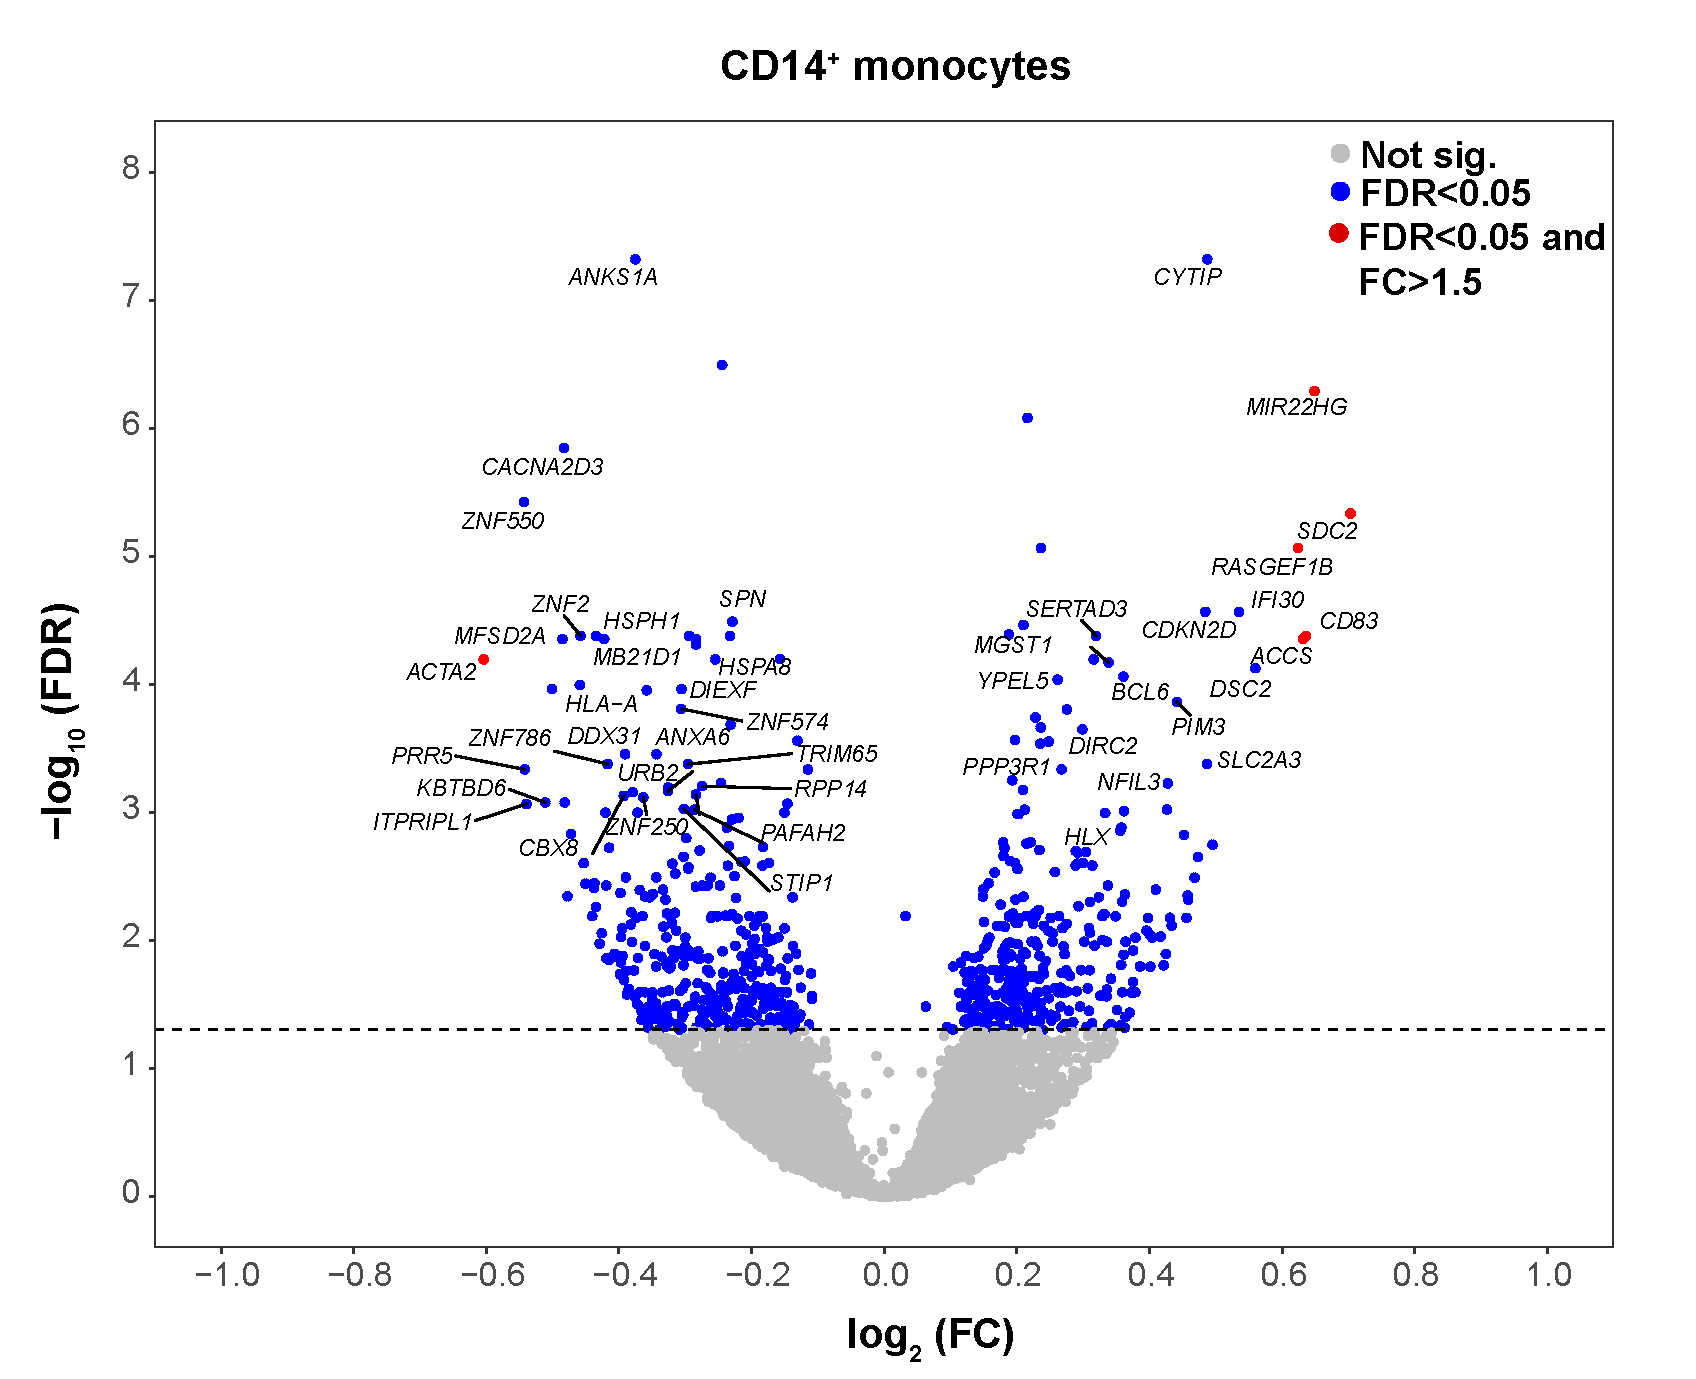
\includegraphics[width=\textwidth]{./Results2/pdfs/RNA_PS_CTL_CD14_volcano_plot}
\caption{\textbf{}}
% The percentage sign indicated that the other subfig goes side by side
\end{subfigure}%
\begin{subfigure}{0.5\textwidth}
\centering
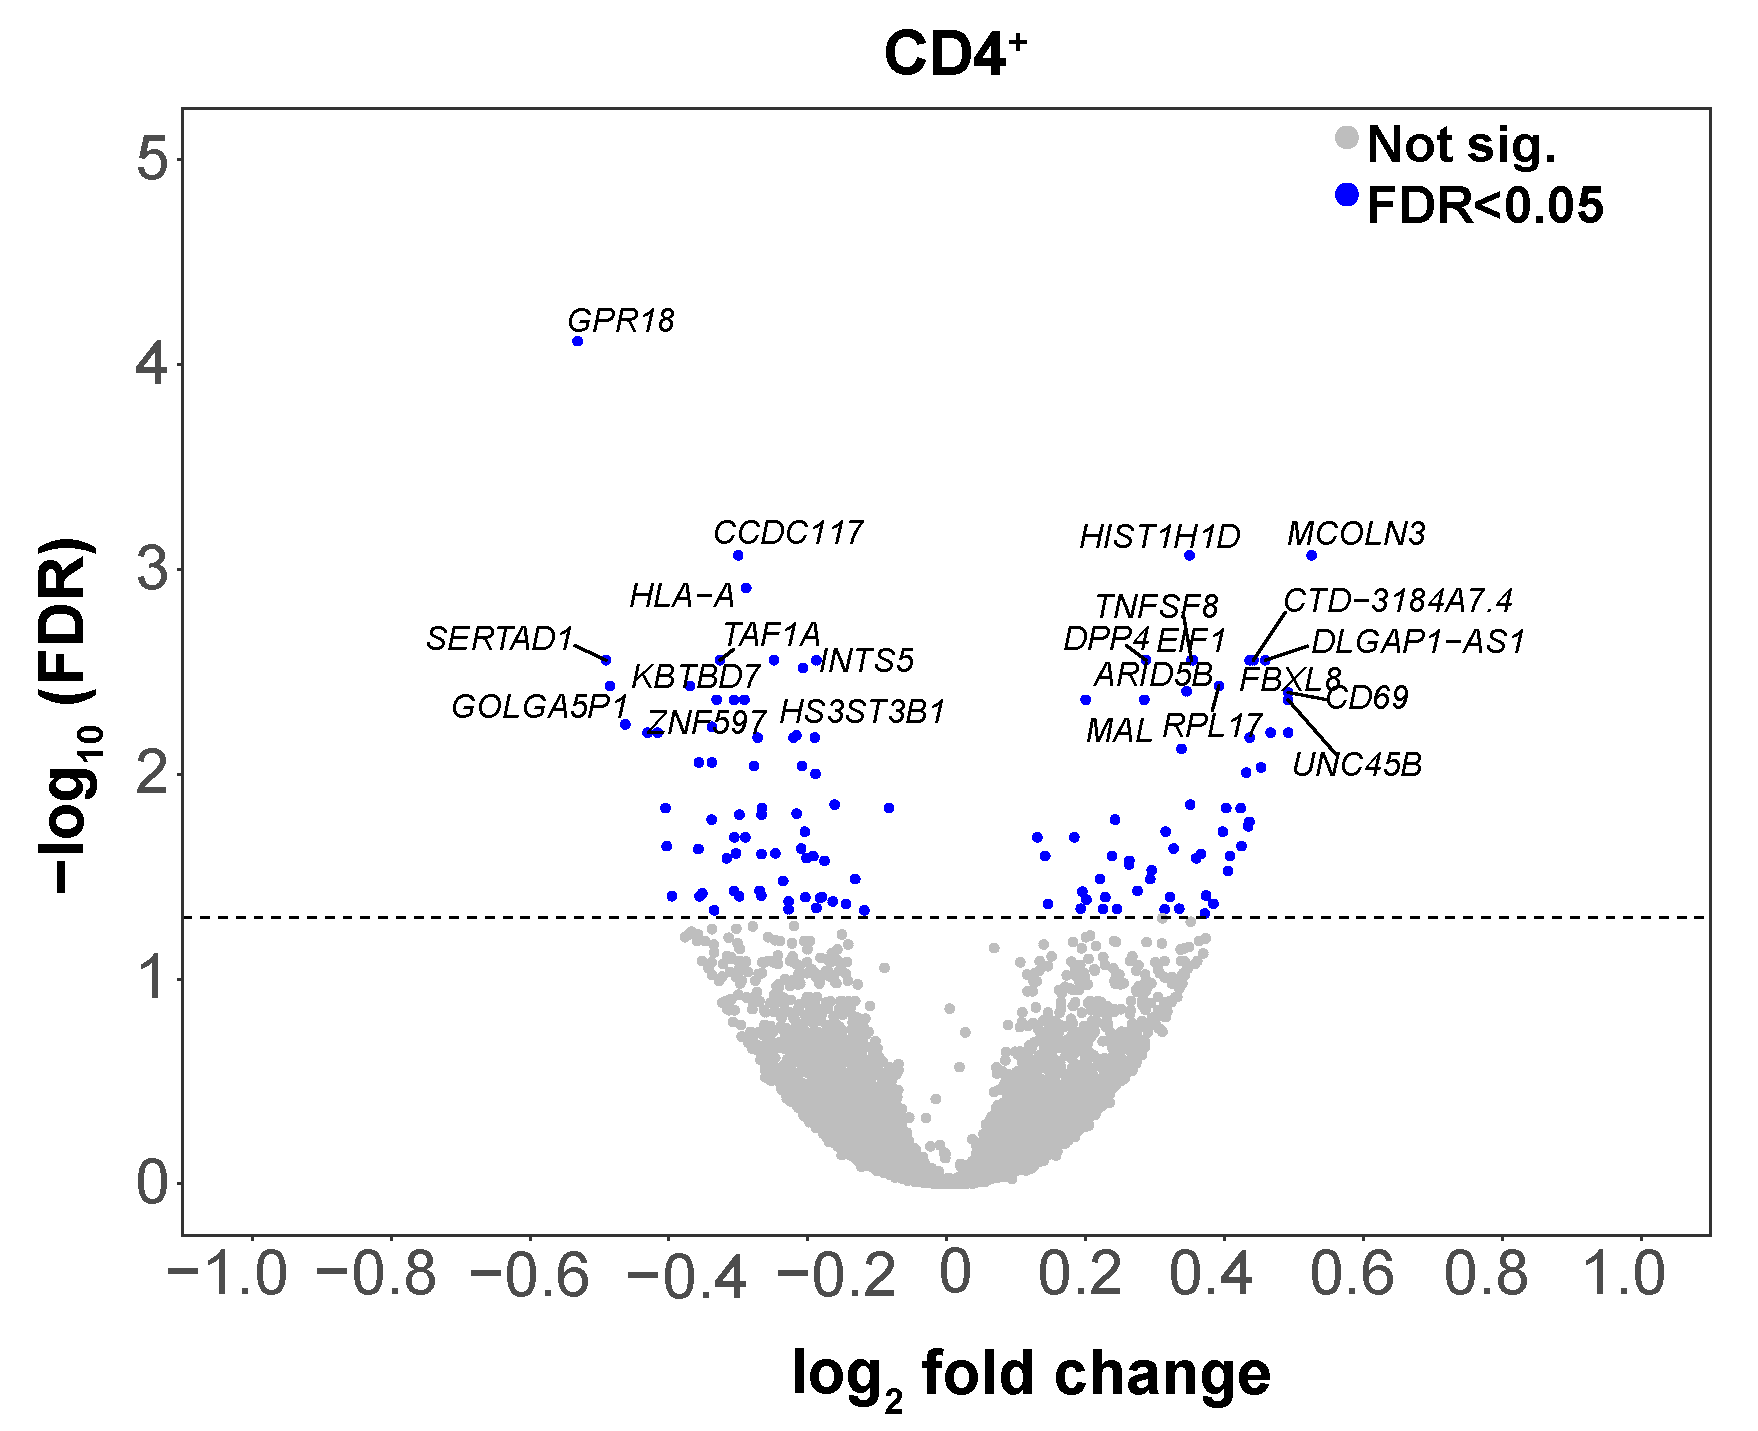
\includegraphics[width=\textwidth]{./Results2/pdfs/RNA_PS_CTL_CD4_volcano_plot}
\caption{\textbf{}}
\end{subfigure}
\begin{subfigure}{0.5\textwidth}
\centering
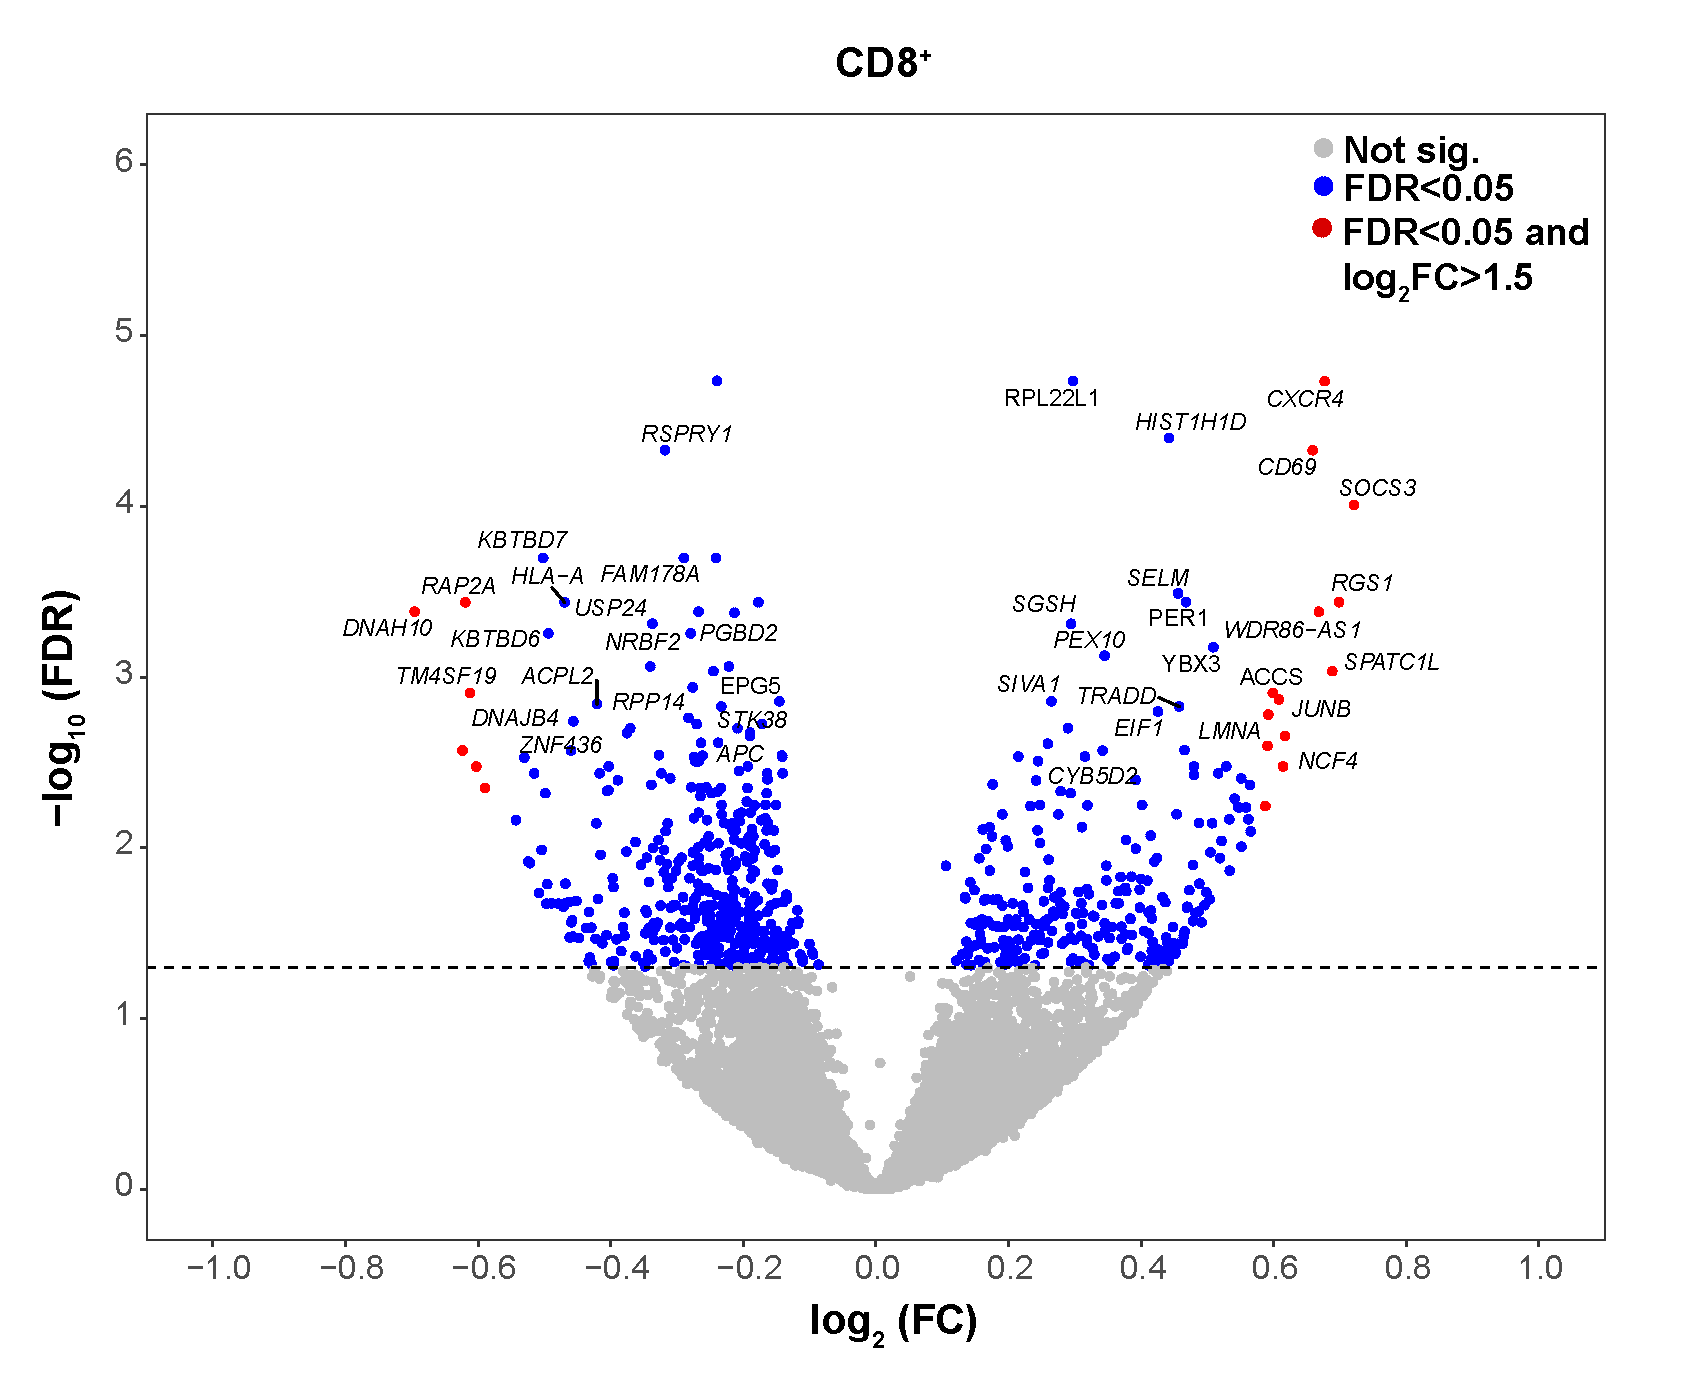
\includegraphics[width=\textwidth]{./Results2/pdfs/RNA_PS_CTL_CD8_volcano_plot}
\caption{\textbf{}}
% The percentage sign indicated that the other subfig goes side by side
\end{subfigure}%
\begin{subfigure}{0.5\textwidth}
\centering
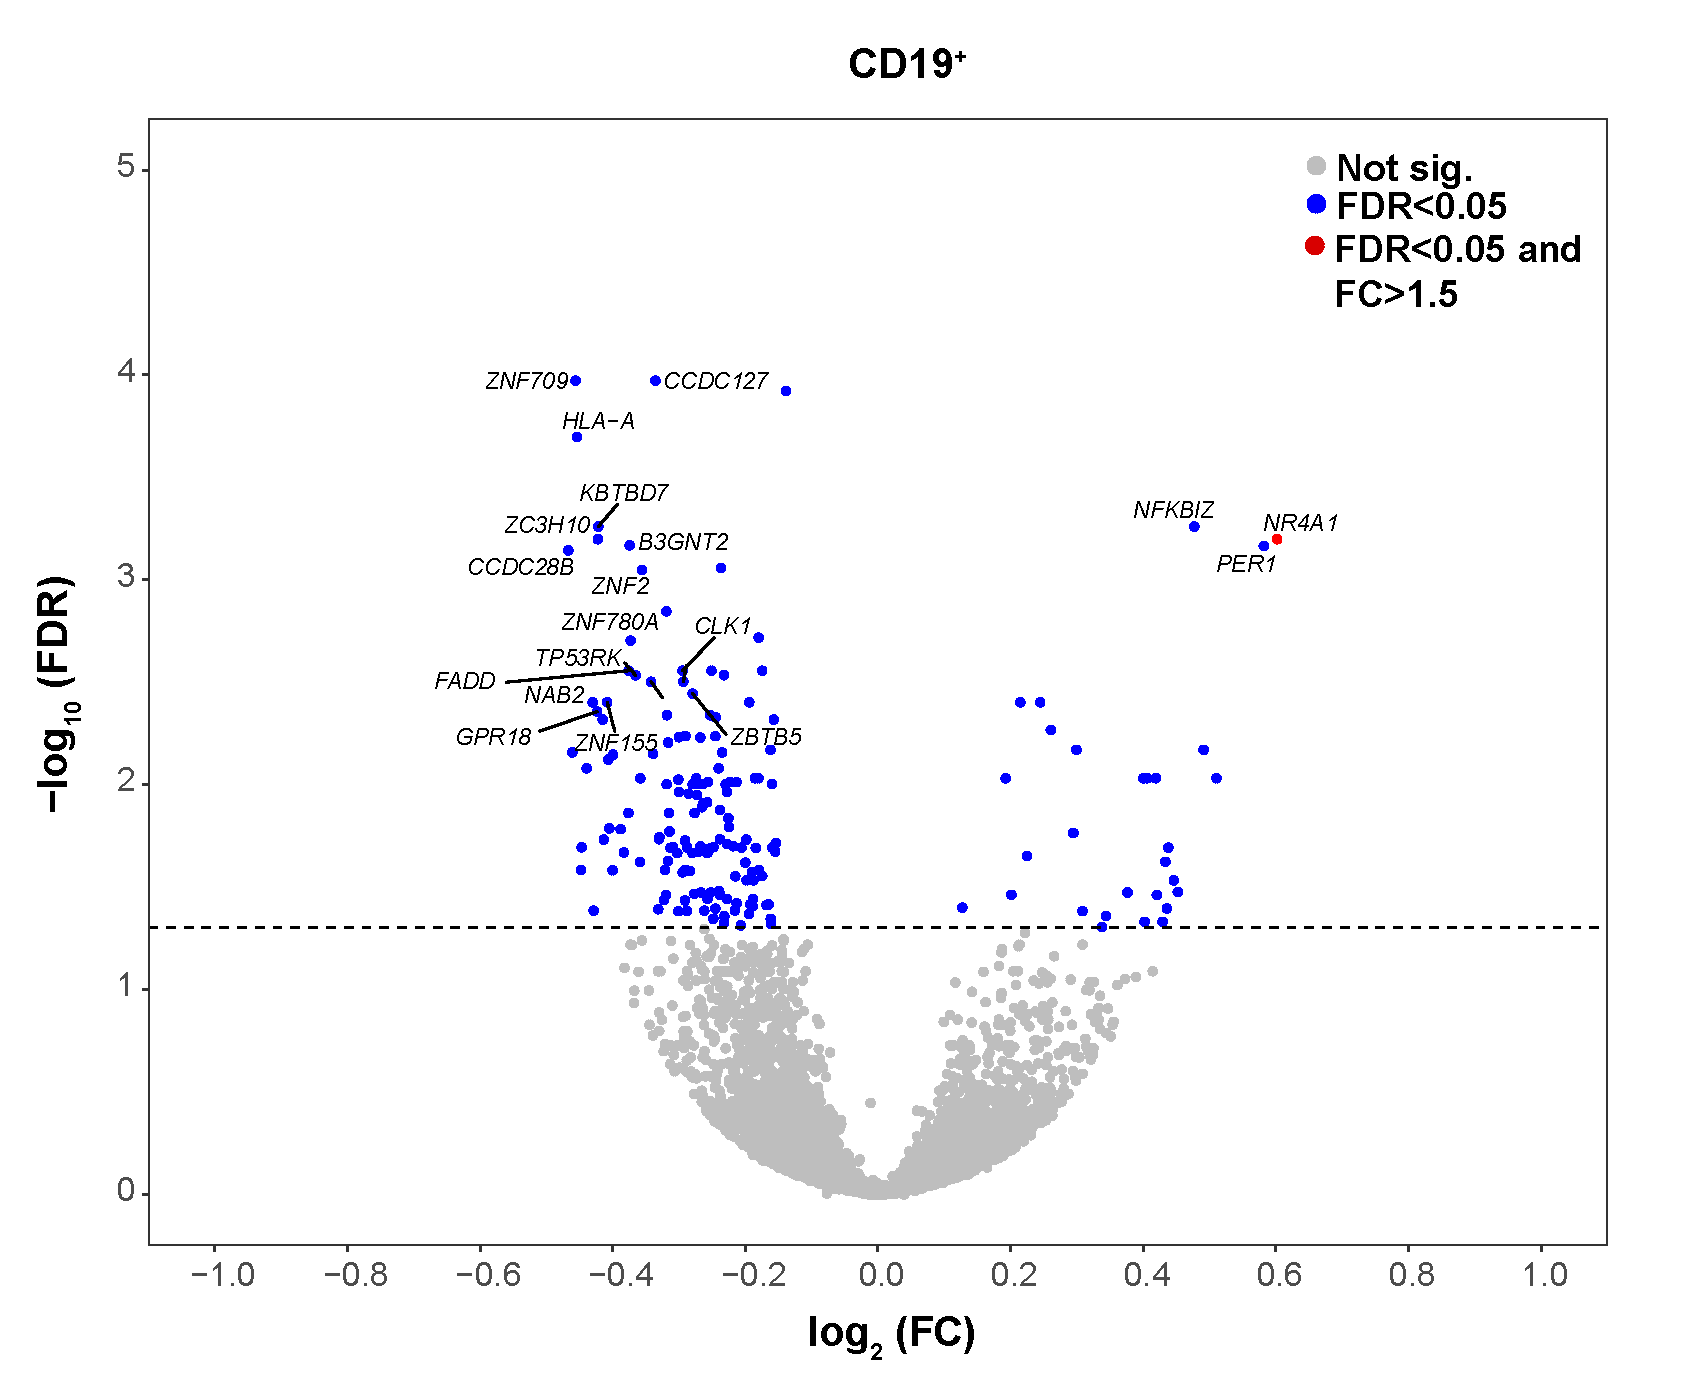
\includegraphics[width=\textwidth]{./Results2/pdfs/RNA_PS_CTL_CD19_volcano_plot}
\caption{\textbf{}}
\end{subfigure}
\caption[Magnitude and significance of the gene expression changes between psoriasis patients and healthy controls in four immune cell types.]{\textbf{Magnitude and significance of the gene expression changes between psoriasis patients and healthy controls in four immune cell types.} Volcano plots for the results of the DGE analysis in a) CD14$^+$ monocytes, b) CD4$^+$, c) CD8$^+$ and d) CD19$^+$ cells. For each gene, the log$_2$(FC) represents the change in expression for that gene in the psoriasis group with reference to the healthy controls. Significant DEGs (FDR$<$0.05) in blue for FC $<$1.5 and red for FC $>$1.5. The volcano plots include mRNAs and lncRNAs species.}
\label{figure:RNAseq_PS_CTL_volcano_plots}
\end{figure} 


Some of the DEGs across the four cell types overlapped DEGs from the two most comprehensive studies comparing expression of PBMCs isolated from psoriasis patients and healthy controls \parencite{Lee2009,Coda2012}. The greatest overlap (7 genes) was found between the DEGs in CD14$^+$ monocytes and those identified by Coda \textit{et al.}, 2012. However, 5 out of 7 presented opposite directionality. One of those genes dysregulated in the same direction was ubiquitin conjugating enzyme E2 D1 (\textit{UBE2D1}), which mediates, for example, ubiquitination of the TNF receptor-associated factor 6 (TRAF6) protein \parencite{Gru2008}. The greatest overlap with the Lee and colleagues DEGs was found for CD8$^+$ cells (3 genes) in the same direction. Similarly, only one overlap (\textit{NAMPT}) was found with the psoriasis DEGs in a study comparing PBMC transcriptional profiles of three inflammatory diseases (IBD, RA and psoriasis)\parencite{Mesko2010}. The nicotinamide phosphoribosyltransferase\textit{NAMPT}, involved in metabolism and stress response, was up-regulated in our CD14$^+$ monocytes as well as in PBMCs from the three phenotypes studied by Mesko and colleagues, suggesting its role as a marker of inflammation rather than marker for psoriasis.
%For example, CDC like kinase 1 (\textit{CLK1}) involved in protein splicing was downregulated in this CD8$^+$ data set and in the Lee PBMCs in patients when compared to controls and its deficiency has been shown to lead to neuro-inflammation in mice \parencite{Gu2017}. Similarly, only one overlap was found with the psoriasis DEGs in a study comparing PBMC transcriptional profiles of three inflammatory diseases (IBD, RA and psoriasis)\parencite{Mesko2010}. This was for the nicotinamide pPhosphoribosyltransferase (\textit{NAMPT}) gene involved in metabolism and stress response, which was up-regulated in our CD14$^+$ monocytes as well as in PBMCs from psoriasis, IBD and RA patients, suggesting its role as a marker of inflammation rather than marker for psoriasis.

An overlap between the significant DEGs (FDR$<$0.05) across the four cell types and a list of the genes putatively associated with psoriasis GWAS hits from the NHGRI-EBI catalog (https://www.ebi.ac.uk/gwas) curated to include other genes from more recent studies was performed (Table \ref{tab:RNAseq_PS_CTL_GWAS_overlap}). CD8$^+$ was the cell type with the largest number of DEGs (7 hits) overlapping with putative GWAS genes, followed by CD14$^+$ monocytes and CD4$^+$ (3 hits each). Some of those genes were found in more than one cell type, including \textit{NFKBIA}, \textit{TNFAIP3} and \textit{NFKBIZ}, amongst others.  


\begin{table}[htbp]
%\setlength{\tabcolsep}{20pt} only to stretch the columns if you want
%\renewcommand{\arraystretch}{1.5}
\centering
\begin{tabular}{@{} c c c c}
\toprule
\textbf{Cell type}   & \textbf{Number of GWAS}   & \textbf{Up-regulated}   & \textbf{Down-regulated}  \\
										 & \textbf{overlaps}         & \textbf{genes}          &\textbf{genes} \\
\midrule
\midrule
CD14$^+$             & 3  & \textit{NFKBIA}                                   & \textit{IL23A}, \textit{FASLG}\\                 
tCD4$^+$              & 3  & \textit{TNFAIP3}, \textit{NFKBIZ}                 & \textit{FASLG} \\
tCD8$^+$              & 7  & \textit{TNFAIP3}, \textit{NFKBIA}, \textit{ETS1}, & \textit{B3GNT2}, \textit{FASLG} \\ 
                     &    & \textit{SOCS1},\textit{NFKBIZ}                    &  \\ 
CD19$^+$             & 2  & \textit{NFKBIZ}                                   & \textit{B3GNT2}\\
\bottomrule 
\end{tabular}
\medskip %gap
\caption[Overlap between putative psoriasis GWAS genes and the reported significantly DEGs in CD14$^+$ monocytes, CD4$^+$, CD8$^+$ and CD19$^+$ cells.]{\textbf{Overlap between putative psoriasis GWAS genes and the reported significantly DEGs in CD14$^+$ monocytes, CD4$^+$, CD8$^+$ and CD19$^+$ cells.} DEGs list based on FDR$<$0.05.}
\label{tab:RNAseq_PS_CTL_GWAS_overlap}
\end{table}
\bigskip %bigger spac


\subsubsection{The role of lncRNAs in psoriasis circulating immune cells}

In addition to protein coding genes, some of the DEGs identified were classified as lncRNAs. tCD8$^+$ and CD14$^+$ monocytes were the two cell types presenting the largest number of dysregulated lncRNAs between psoriasis patients and controls (Table \ref{tab:RNAseq_PS_CTL_differential_analysis_results}). In contrast, CD19$^+$ was the cell type showing the lowest number of lncRNAs differentially expressed. Only one lncRNA, \textit{RP11-218M22.1} appeared to be dysregulated between psoriasis and healthy controls in all the cell types. 

The differentially expressed lncRNAs in this study were overlapped with the 259 lncRNAs identified as dysregulated in PBMCs when comparing PsA patients versus healthy controls by Dolcino \textit{et al.}, 2018 (Table \ref{tab:RNAseq_PS_CTL_lncRNAs_annotation}). The largest overlap was found in CD14$^+$ monocytes, where four of the differentially expressed lncRNAs were also reported by Dolcino and colleagues. However, \textit{HOTAIRM1} and \textit{ILF3-AS1} were up-regulated in psoriasis CD14$^+$ monocytes when compared to controls but appeared down-regulated in PsA PBMCs. 


\begin{table}[htbp]
%\setlength{\tabcolsep}{20pt} only to stretch the columns if you want
%\renewcommand{\arraystretch}{1.5}
\centering
\begin{tabular}{@{} c c c}
\toprule
\textbf{Cell type}   & \textbf{LncRNAs with}             &\textbf{LncRNAs overlapping}  \\
                     & \textbf{functional interactions}  &\textbf{Dolcino \textit{et al.},2018}   \\
\midrule
\midrule
CD14$^+$             & 24  & 4 (\textit{HOTAIRM1}$^{\ast}$, \textit{ILF3-AS1}$^{\ast}$, \\
                     &     & \textit{MMP24-AS1}, \textit{RP11-325F22.2})\\                 
tCD4$^+$             & 12  & 1 (\textit{MMP24-AS1}) \\
tCD8$^+$             & 21  & 1(\textit{CTB-25B13.12})\\
CD19$^+$             & 5   & 0\\
\bottomrule 
\end{tabular}
\medskip %gap
\caption[Functional interactions and overlap with another study for the differentially expressed lncRNAs in each cell type.]{\textbf{Functional interactions and overlap with another study for the differentially expressed lncRNAs in each cell type.}For each cell type the number of differentially expressed lncRNAs (FDR$<$0.05) for which a functional interaction has been experimentally validated based on NPInter database is shown. NPInter documents functional interactions between noncoding RNAs (except tRNAs and rRNAs) and biomolecules (proteins, RNAs and DNAs) which have published experimental validation. This table also records the number of differentially expressed lncRNAs overlapping with the Dolcino \textit{et al.}, 2018 study, where PBMCs from PsA patients and healthy controls are contrasted.($^{\ast}$) indicates dysregulation in the opposite direction between this data and Dolcino \textit{et al.}.}
\label{tab:RNAseq_PS_CTL_lncRNAs_annotation}
\end{table}
\bigskip %bigger spac

The number of differentially expressed lncRNAs for which a functional interaction had been experimentally found was investigated using NPInter database , which retrieves functional interactions between non-coding RNAs and biomolecules (proteins, RNAs and DNAs) which have been published \parencite{Hao2016}. The majority of the differentially expressed lncRNAs (FDR$<$0.05) in all the cell type were found to have a functional interacting partner.


%The vast majority of the dysregulated lncRNAs between patients and controls at FDR$<$0.05 were functionally uncharacterised, complicating the interpretation of these results. 

Amongst the characterised lncRNAs dysregulated between psoriasis and controls CD14$^+$ monocytes were the negative regulator of antiviral response (\textit{DYNLL1-AS1} or \textit{NAV}), the HOXA transcript antisense RNA myeloid-specific 1 (\textit{HOTAIRM1}) and the nuclear paraspeckle assembly transcript 1 (\textit{NEAT1}). \textit{DYNLL1-AS1} has been shown to affect the histone modifications of some critical IFN-stimulated genes (ISGs) including \textit{IFITM3} and \textit{MxA} leading to down-regulation of their expression \parencite{Ouyang2014}. In this data, \textit{DYNLL1-AS1} appeared down-regulated in CD14$^+$ monocytes from psoriasis patients when compared to controls but no up-regulation of \textit{IFITM3} and \textit{MxA} was found. Conversely, \textit{HOTAIRM1} appeared to be up-regulated in the CD14$+$ monocytes from psoriasis patients (Figure \ref{figure:RNAseq_PS_CTL_CD14_expression_HOTAIRM_UPF1} a). The experimentally validated target for \textit{HOTAIRM1} reported by NPInter database was the RNA helicase and ATPase \textit{UPF1} \parencite{Hao2016}, which was found to be down-regulated in CD14$^+$ monocytes in psoriasis versus control samples in this data (Figure \ref{figure:RNAseq_PS_CTL_CD14_expression_HOTAIRM_UPF1} b). Lastly, \textit{NEAT1} was also up-regulated in psoriasis patients compared to controls and had also been found to be up-regulated in a study in SLE CD14$^+$ monocytes \parencite{Zhang2016}.

%The negative regulator of antiviral response \textit{DYNLL1-AS1} (or \textit{NAV}), which has been shown to affect the histone modifications of some critical IFN-stimulated genes (ISGs), such as \textit{IFITM3} and \textit{MxA} leading to down-regulation of their expression \parencite{Ouyang2014}. In this data, \textit{DYNLL1-AS1} was down-regulated indicating lack of one of the negative regulators of the IFN response, notwithstanding the reverse  IFN-$\gamma$ signature observed in the pathway enrichment analysis. Another interesting dysregulated lncRNA in CD14$^+$ monocytes was the HOXA transcript antisense RNA myeloid-specific 1\textit{HOTAIRM1}. In a study using PsA PBMCs \textit{HOTAIRM1} was found to be down-regulated and connected to the expression of the RNA helicase and ATPase \textit{UPF1} \parencite{Dolcino2018}. \textit{UPF1} is involved in nonsense-mediated decay and in partnership with the monocyte chemotactic protein-1-induced protein-1 (\textit{MCPIP1}) gene drives degradation of inflammation-related mRNAs to ensure maintenance of homeostasis \parencite{Mino2015}. In this present study, \textit{HOTAIRM1} appeared to be up-regulated in the CD14$+$ monocytes from psoriasis patients (Figure \ref{figure:RNAseq_PS_CTL_CD14_expression_HOTAIRM_UPF1} a) and this was consistent with significant down-regulation of \textit{UPF1} in the same cell type (Figure \ref{figure:RNAseq_PS_CTL_CD14_expression_HOTAIRM_UPF1} b), suggesting impairment of this homeostatic mechanisms in the psoriasis patients. The last relevant lncRNA differentially expressed in monocytes was \textit{NEAT1}, which was up-regulated in the patients  compared to the controls. \textit{NEAT1} has been reported to also be up-regulated in SLE CD14$^+$ monocytes and knocking it down has revealed impairment of the TLR-4 signalling and down-regulation of inflammatory genes including IL-6 and CXCL10 \parencite{Zhang2016}.


 \begin{figure}[htbp]
\centering
\begin{subfigure}{0.45\textwidth}
\centering
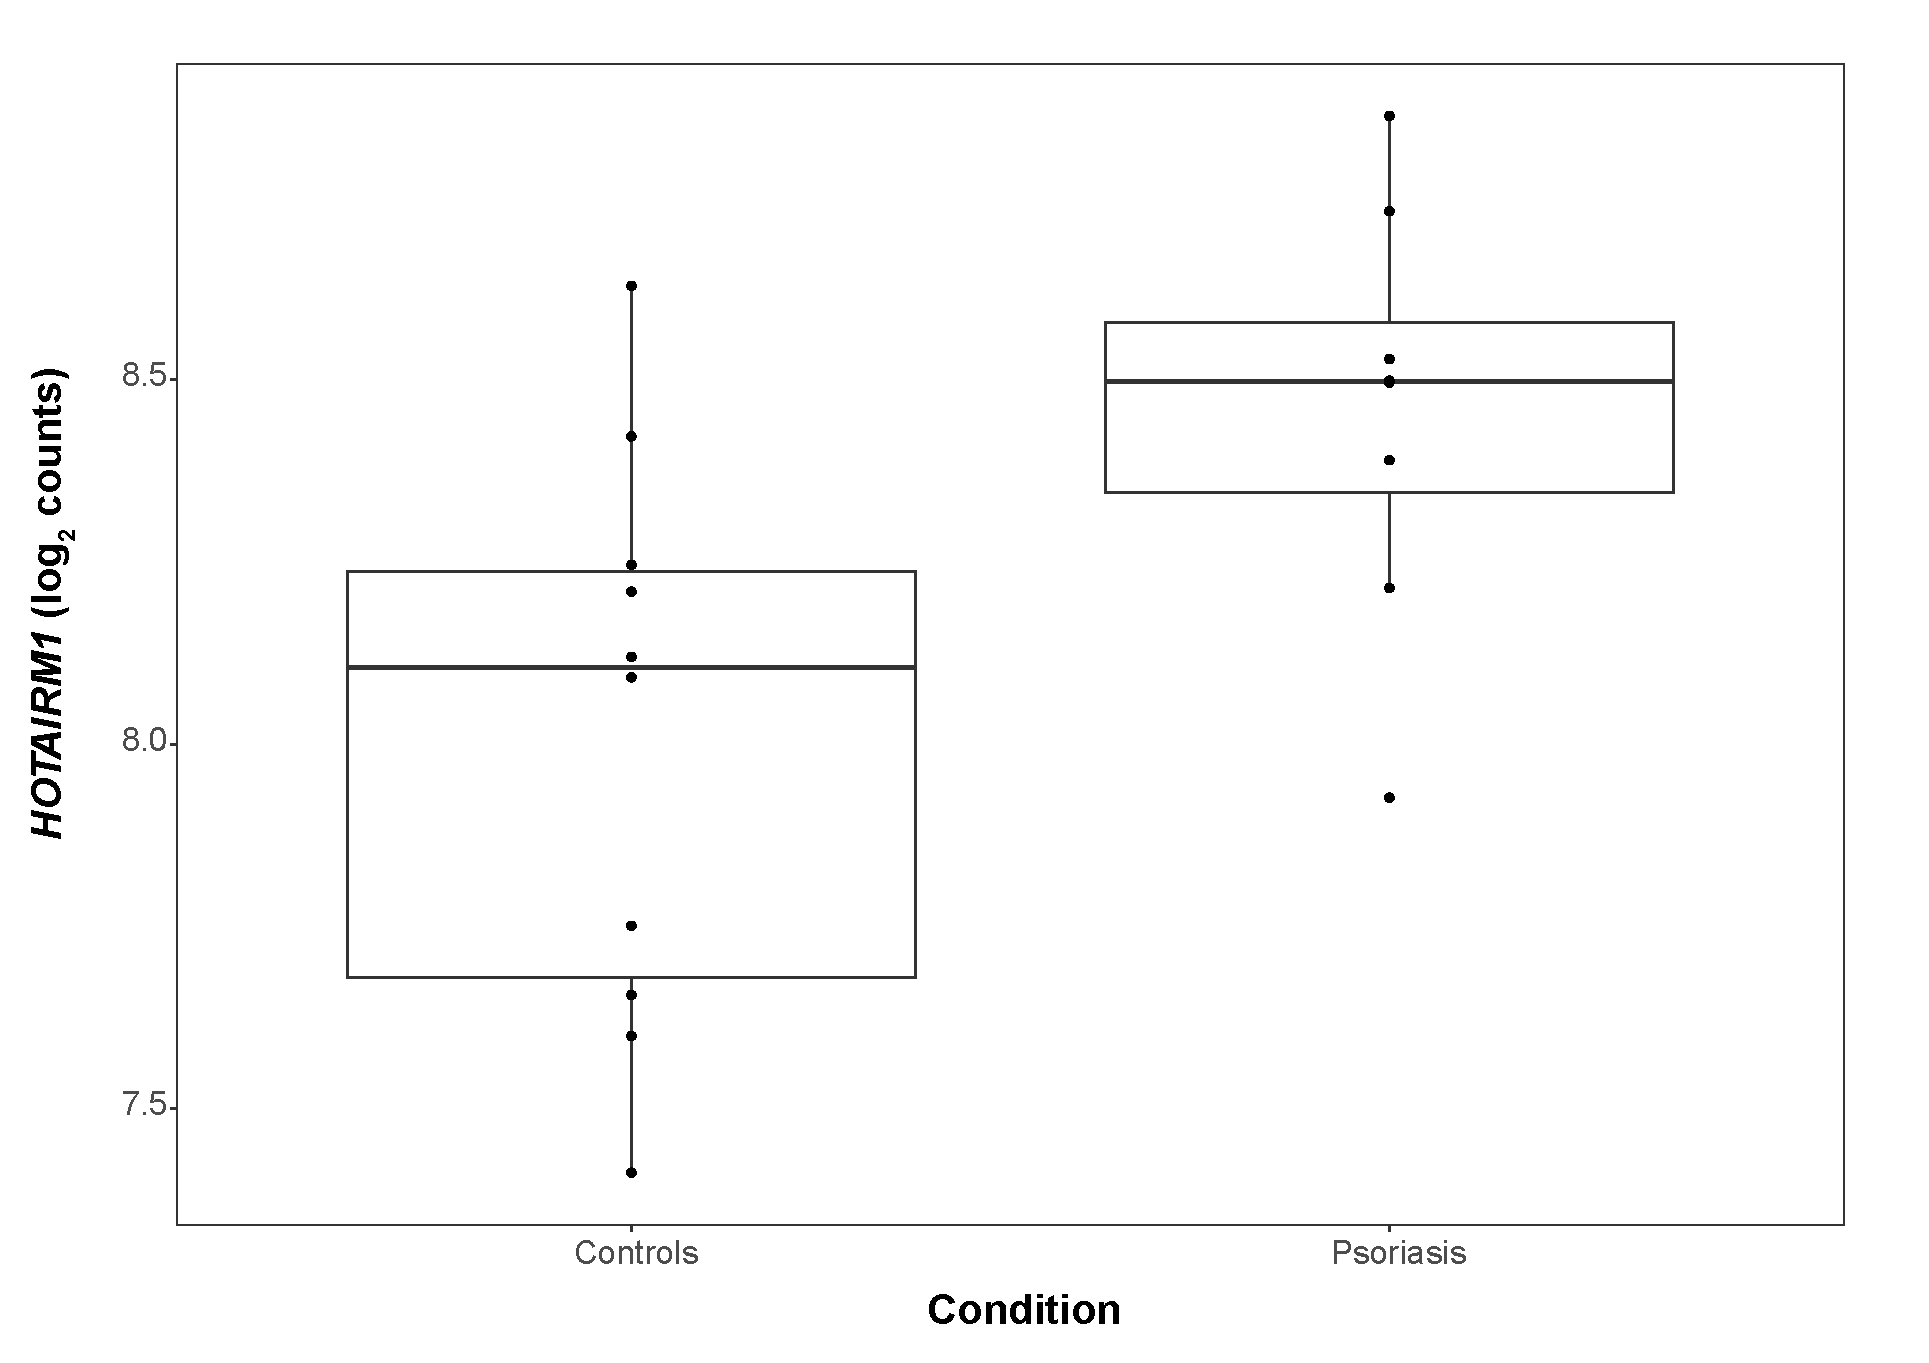
\includegraphics[width=\textwidth]{./Results2/pdfs/RNAseq_PS_CTL_lncRNA_HOTAIRM1_CD14}
\caption{\textbf{}}
% The percentage sign indicated that the other subfig goes side by side
\end{subfigure}%
\begin{subfigure}{0.45\textwidth}
\centering
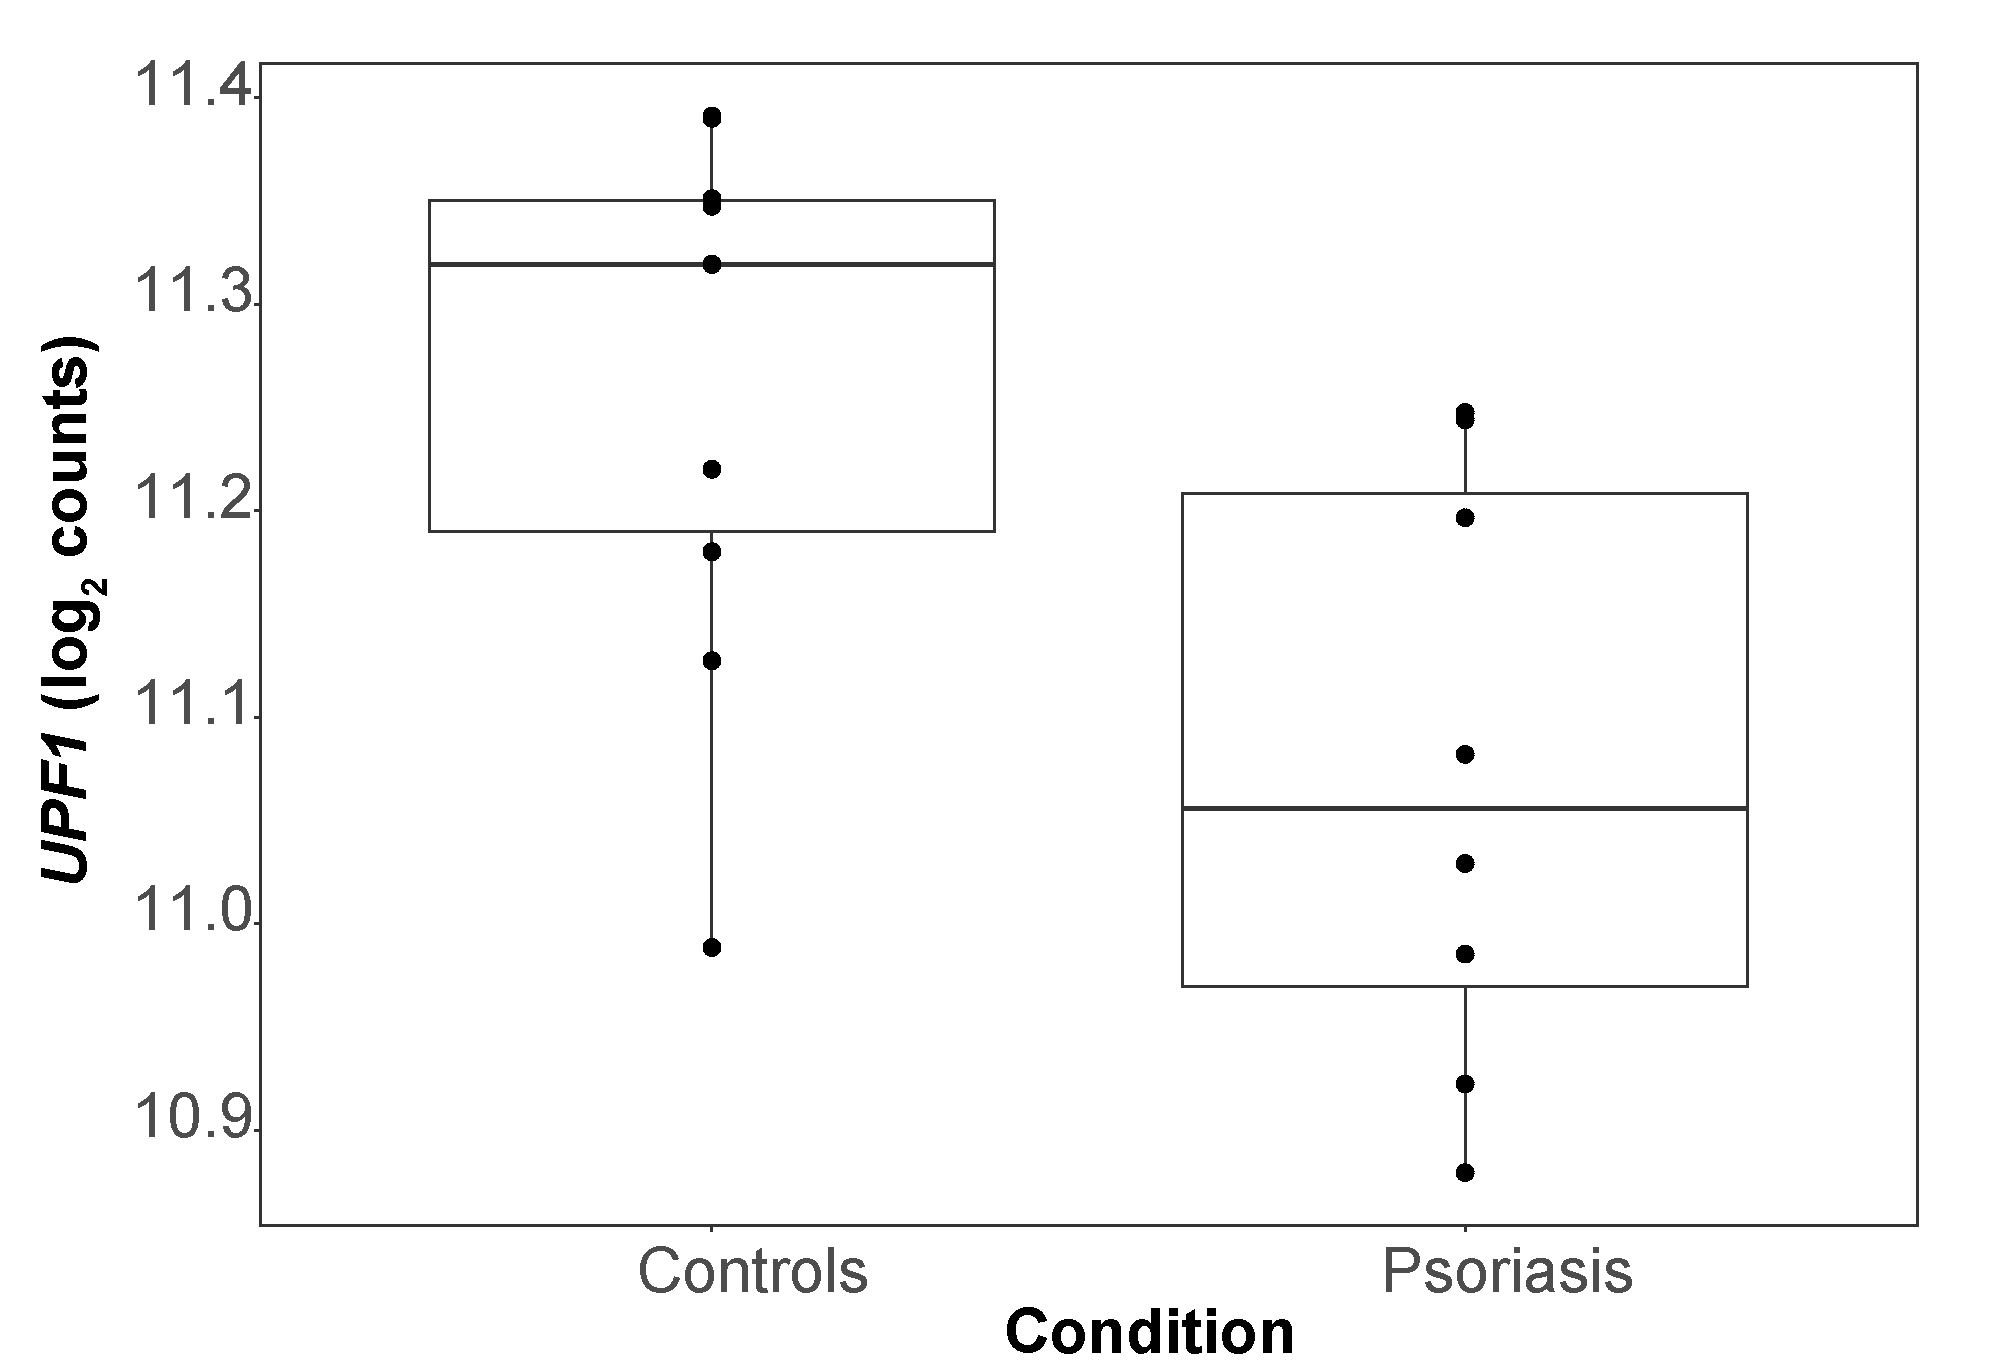
\includegraphics[width=\textwidth]{./Results2/pdfs/RNAseq_PS_CTL_lncRNA_UPF1_CD14}
\caption{\textbf{}}
\end{subfigure}
\caption[RNA-seq expression levels of the lncRNA \textit{HOTAIRM1} and its experimentally validated target \textit{UPF1} in psoriasis and healthy controls CD14$^+$ monocytes.]{\textbf{RNA-seq expression levels of the lncRNA \textit{HOTAIRM1} and its experimentally validated target \textit{UPF1} in psoriasis and healthy controls CD14$^+$ monocytes.} Expression is illustrated as the log$_2$ of the normalised read counts mapping to a) the lncRNA \textit{HOTAIRM1} and b) \textit{UPF1}, which has been experimentally identified as one of the genes regulated by this lncRNA according to NPInter database.}
\label{figure:RNAseq_PS_CTL_CD14_expression_HOTAIRM_UPF1}
\end{figure} 


For tCD8$^+$ cells, the most relevant non-coding RNA was the miR \textit{MIR146A}, which was captured in the standard RNA library preparation. \textit{MIR146A} has been characterised to have a role in negative regulation of innate immunity, inflammatory response and antiviral pathway and was found to be down-regulated in psoriasis patients when compared to controls. %Molecular studies have suggested a role for miR-146a as a negative regulator of the TLR-4 pathway \parencite{Taganov2006}. 
Other lncRNAs were found to be dysregulated in more than one cell type. For example, \textit{KCNQ1OT1} was downregulated in both, tCD4$^+$ and tCD8$^+$ cells. Dysregulated expression of this lncRNA has been reported in Beckwith-Wiedemann syndrome consisting of a loss-of-imprinting paediatric overgrowth disorder with some skin features such as creases or pits in the skin near the ears \parencite{Pandei2008}.


%This is in line with findings in serum from SLE and early RA patients \parencite{Wang2012,Filkova}. In contrast, trancriptomic studies using PBMCs from plaque psoriasis and also similar studies in RA (including PBMCs, SFMCs and CD4$^+$ isolated from both tissues, amongst others) have reported increased levels of miR-146a in patients when compared to controls \parencite{Ele-Refaei2015,Churov2015}. Molecular studies have suggested a role for miR-146a as a negative regulator of the TLR-4 pathway \parencite{Taganov2006}. This study demonstrated regulation of \textit{MIR146A} expression by NF-$\kappa$B upon inflammation as well as \textit{in vitro} targeting of the 3'UTR of \textit{TRAF6} and IL-1 receptor-associated kinase 1 (\textit{IRAK1}) genes. These are adaptor molecules that lead to activation of kinases from the TLR-4 pathway that eventually lead to translocation of NF-$\kappa$B and AP-1 into the nucleus and transcriptional up-regulation of inflammatory genes. 

%Other lncRNAs were found to be dysregulated in more than one cell type. For example, \textit{KCNQ1OT1} was downregulated in both, CD4$^+$ and CD8$^+$ cells. Dysregulated expression of this lncRNA has been reported in Beckwith-Wiedemann syndrome consisting of a loss-of-imprinting paediatric overgrowth disorder with some skin features such as creases or pits in the skin near the ears \parencite{Pandei2008}. \textit{KCNQ1OT1} has been reported to interact with DNA methyltransferases and also to facilitate the interaction of these enzymes with the chromatin, leading to misregulation of imprinted loci.



\subsubsection{Pathway enrichment analysis for the DEGs}

In order to better understand the biological role of the significantly modulated genes, pathway enrichment analysis was performed for each cell type. The moderated FCs in the DGE analysis illustrated in the volcano plots suggest that the differences between patients and controls in these circulating immune cells are discrete. Nevertheless, moderate differences may have an important impact on their phenotype for infiltration and activation in the skin. Therefore, exploratory pathway analysis was conducted using DEG with FDR$<$0.05 and no FC cut off. Biologically relevant pathways appeared to be significantly enriched (FDR$<$0.01) for CD14$^+$ monocytes and CD8$^+$ cells DEGs (Table \ref{tab:tab:RNAseq_PS_CTL_pathway_enrichment} and \ref{tab:RNAseq_PS_CTL_additional_pathways}). In CD19$^+$ cells, only one pathway (“generic transcription”) appeared to be significantly enriched for DEGs in this cell type. In contrast, in CD4$^+$ cells modulated genes between psoriasis patients and controls were not enriched for any pathway. 

\begin{table}[htbp]
%\setlength{\tabcolsep}{20pt} only to stretch the columns if you want
%\renewcommand{\arraystretch}{1.5}
\centering
\begin{tabular}{@{} c c}
\toprule
\textbf{Cell type} & \textbf{Pathways} \\
\midrule
\midrule
                      & MAPK signalling \\
                      & IL-12 mediated signaling events \\
				              & Th-1 and Th-2 cell differentiation \\
CD14$^+$ monocytes    & Th-17 cell differentiation \\
				              & TCR signalling \\
				              & Platelet-derived growth factor (PDGF-$\beta$) signalling\\
				              & Forkhead box O (FoxO) signalling \\
\midrule				
CD8$^+$  & Osteoclast differentiation \\
         & MAPK signalling \\
				 & TNF signalling \\
         & IL-12 mediated signalling events \\
				 & NF-$\kappa$B signalling \\
				 & Chemokine signalling \\
\bottomrule
\end{tabular}
\medskip %gap
\caption[Most relevant pathways enriched for DEGs between psoriasis patients and healthy controls in CD14$^+$ monocytes and CD8$^+$ cells.]{\textbf{Most relevant pathways enriched for DEGs between psoriasis patients and healthy controls in CD14$^+$ monocytes and CD8$^+$ cells.} The enrichment analysis was conducted using significantly DEGs FDR$<$0.05 and no FC threshold. Enriched pathways had FDR$<$0.01 and a minimum of ten gene members overlapping with DEGs for that particular cell type.}
\label{tab:RNAseq_PS_CTL_pathway_enrichment}
\end{table}


Two of the significant enriched pathways, MAPK signalling and IL-12 mediated signalling, were found to be enriched for CD14$^+$ monocytes and CD8$^+$ cells DEGs (Table \ref{tab:tab:RNAseq_PS_CTL_pathway_enrichment}). DEGs contributing to the enrichment of this pathway in both cell types included MAPK gene members such as \textit{MAP3K4} and \textit{MAPK14}, both down-regulated in psoriasis when compared to controls. For example, MAP3K4 is a member of the MAPKKK family, which expression is down-regulated in LPS-stimulated PBMCs from CD patients leading to a relative immune deficiency in TLR-mediated cytokine production. Moreover, DGE of members of the dual-specificity phosphatases (DUSP) family, involved in fine-tuning the immune response \parencite{Qian2009}, contributed to the enrichment of the MAPK pathway in CD14$^+$ monocytes and tCD8$^+$ cells. For instance, \textit{DUSP10} was down-regulated in the psoriasis CD14$^+$ monocytes and its knock-out in mice led to enhanced inflammation \parencite{Qian2009}. Conversely, \textit{DUSP4} presented up-regulation in psoriasis tCD8$^+$ when compared to healthy controls and has been demonstrated to have a pro-inflammatory role in a sepsis mice model \parencite{Cornell2010}.

%Enrichment was shared between CD14$^+$ monocytes and CD8$^+$ cells. Some of the DEGs contributing to the enrichment of this pathway in both cell types included MAPK gene members such as \textit{MAP3K4} and \textit{MAPK14}, both down-regulated in psoriasis when compared to controls. Interestingly, MAP3K4 is a member of the MAPKKK family, for which expression is down-regulated in LPS-stimulated PBMCs from CD patients, leading to reduced expression of the cytokine \textit{IL-1A} and a relative immune deficiency in TLR-mediated cytokine production. Moreover, DGE of members of the dual-specificity phosphatases (DUSP) family involved in fine-tuning the immune response \parencite{Qian2009} contribute to the enrichment of the MAPK pathway in CD14$^+$ monocytes and CD8$^+$ cells. \textit{DUSP10} was down-regulated in the psoriasis CD14$^+$ monocytes and could be modulating reactive oxygen species production according to a knock-out mice phenotype presenting enhanced inflammation \parencite{Qian2009}. Conversely, \textit{DUSP4} presented up-regulation in tCD8$^+$ patients when compared to healthy controls and it could represent a pro-inflammatory feature as this gene has been demonstrated to have a role in driving inflammation in a sepsis mice model \parencite{Cornell2010}.  

Regarding enrichment of the IL-12 signalling, CD14$^+$ monocytes from psoriasis presented down-regulation of \textit{STAT4} and \textit{STAT5A} in patients compared to controls. Neither \textit{STAT4} and \textit{STAT5A} were dysregulated in tCD8$^+$ cells between psoriasis and healthy controls. Likewise, \textit{IFNG} expression in psoriasis patients was lower than in healthy controls in tCD8$^+$ cells but changes were not found in CD14$^+$ monocytes. \textit{IL2RA} was also up-regulated in tCD8$^+$ from psoriasis patients when compared to controls, which may enhance formation of the IL2-R$\alpha$ and the signalling by this cytokine involved in effector and regulatory T cell differentiation \parencite{Malek2010}.


%Other interesting pathways enriched for both cell types  included IL-12 mediated signalling (Table \ref{tab:RNAseq_PS_CTL_pathway_enrichment}). IL-12 signalling leads to T cell proliferation and IFN-$\gamma$ production through activation of TFs from the STAT family. Importantly STAT4 is a well-known drug target for psoriasis treatment. Interestingly, CD14$^+$ monocytes from psoriasis presented down-regulation of \textit{STAT4} and \textit{STAT5A} in patients compared to controls. Likewise, \textit{IFNG} expression in psoriasis patients was lower than in healthy controls in CD8$^+$ cells. This phenomenon has been previously observed in macrophages derived from AS patients as well as in an SpA rat model \parencite{Smith2008,Fert2014}. Additionally, \textit{IL2RA} was up-regulated in CD8$^+$ from psoriasis patients when compared to controls, which may enhance formation of the IL2-R$\alpha$ and the signalling by this cytokine involved in effector and regulatory T cell differentiation \parencite{Malek2010}.


The platelet-derived growth factor (PDGF-$\beta$) signalling pathway was only enriched in CD14$^+$ monocytes (Table \ref{tab:RNAseq_PS_CTL_pathway_enrichment}). Within this pathway the \textit{SLA} gene appeared to be down-regulated in psoriasis patients compared to controls. A \textit{SLA} knock-out mouse model has shown impaired IL-12 and TNF-$\alpha$ and failure of T cell stimulation by GM-CSG treated bone marrow-derived DCs \parencite{Liontos2011}.
%https://www.ncbi.nlm.nih.gov/pmc/articles/PMC3884931/
% role of SLA in monocytes http://www.jimmunol.org/content/186/4/1923.long

A number of very relevant inflammatory pathways in psoriasis were enriched only in tCD8$^+$ cells. These included TNF, NF-$\kappa$B and chemokine signalling (Table \ref{tab:RNAseq_PS_CTL_pathway_enrichment}). Due to the close relationship between these three pathways, some DEGs contributed to the enrichment of more than one of them. That was the case for NF-$\kappa$B inhibitor A (\textit{NFKBIA}) and the TNF-$\alpha$ induced protein 3 (\textit{TNFAIP3}) which were unexpectedly up-regulated in tCD8$^+$ cells from psoriasis compared to healthy controls. \textit{NFKBIA} up-regulation contributed to the enrichment of all three pathways (Figure \ref{figure:RNAseq_PS_CTL_CD8_TNF_and_chemokine_pathway_modified} a (in green box and b) and \textit{TNFAIP3} was a member of the TNF and NF-$\kappa$B pathways (Figure \ref{figure:RNAseq_PS_CTL_CD8_TNF_and_chemokine_pathway_modified} a in green box). Interestingly, \textit{NFKBIA} and \textit{TNFAIP3} are two of the psoriasis GWAS associated genes and were also up-regulated in psoriasis CD14$^+$ monocytes and tCD4$^+$ cells, respectively (Table \ref{tab:RNAseq_PS_CTL_GWAS_overlap}).

%Interestingly, \textit{NFKBIA} and \textit{TNFAIP3} were also up-regulated in CD14$^+$ monocytes and CD4$^+$ cells. \textit{NFKBIA} codes for the NF-$\kappa$B inhibitor alpha (I$\kappa$B$\alpha$) which binds to the NF-$\kappa$B subunits preventing them from translocation to the nucleus by masking a nuclear localisation signal (NLS). Similarly, \textit{TNFAIP3} codes for the zinc finger protein and ubiqitin-editing enzyme A20, that inhibits both NF-$\kappa$B signalling and TNF-mediated apoptosis. Unexpectedly, these two genes with an anti-inflammatory role appeared to be up-regulated in psoriasis patients when compared to controls in two of the studied cell types. 


\begin{figure}[htbp]
\centering
\begin{subfigure}{0.8\textwidth}
\centering
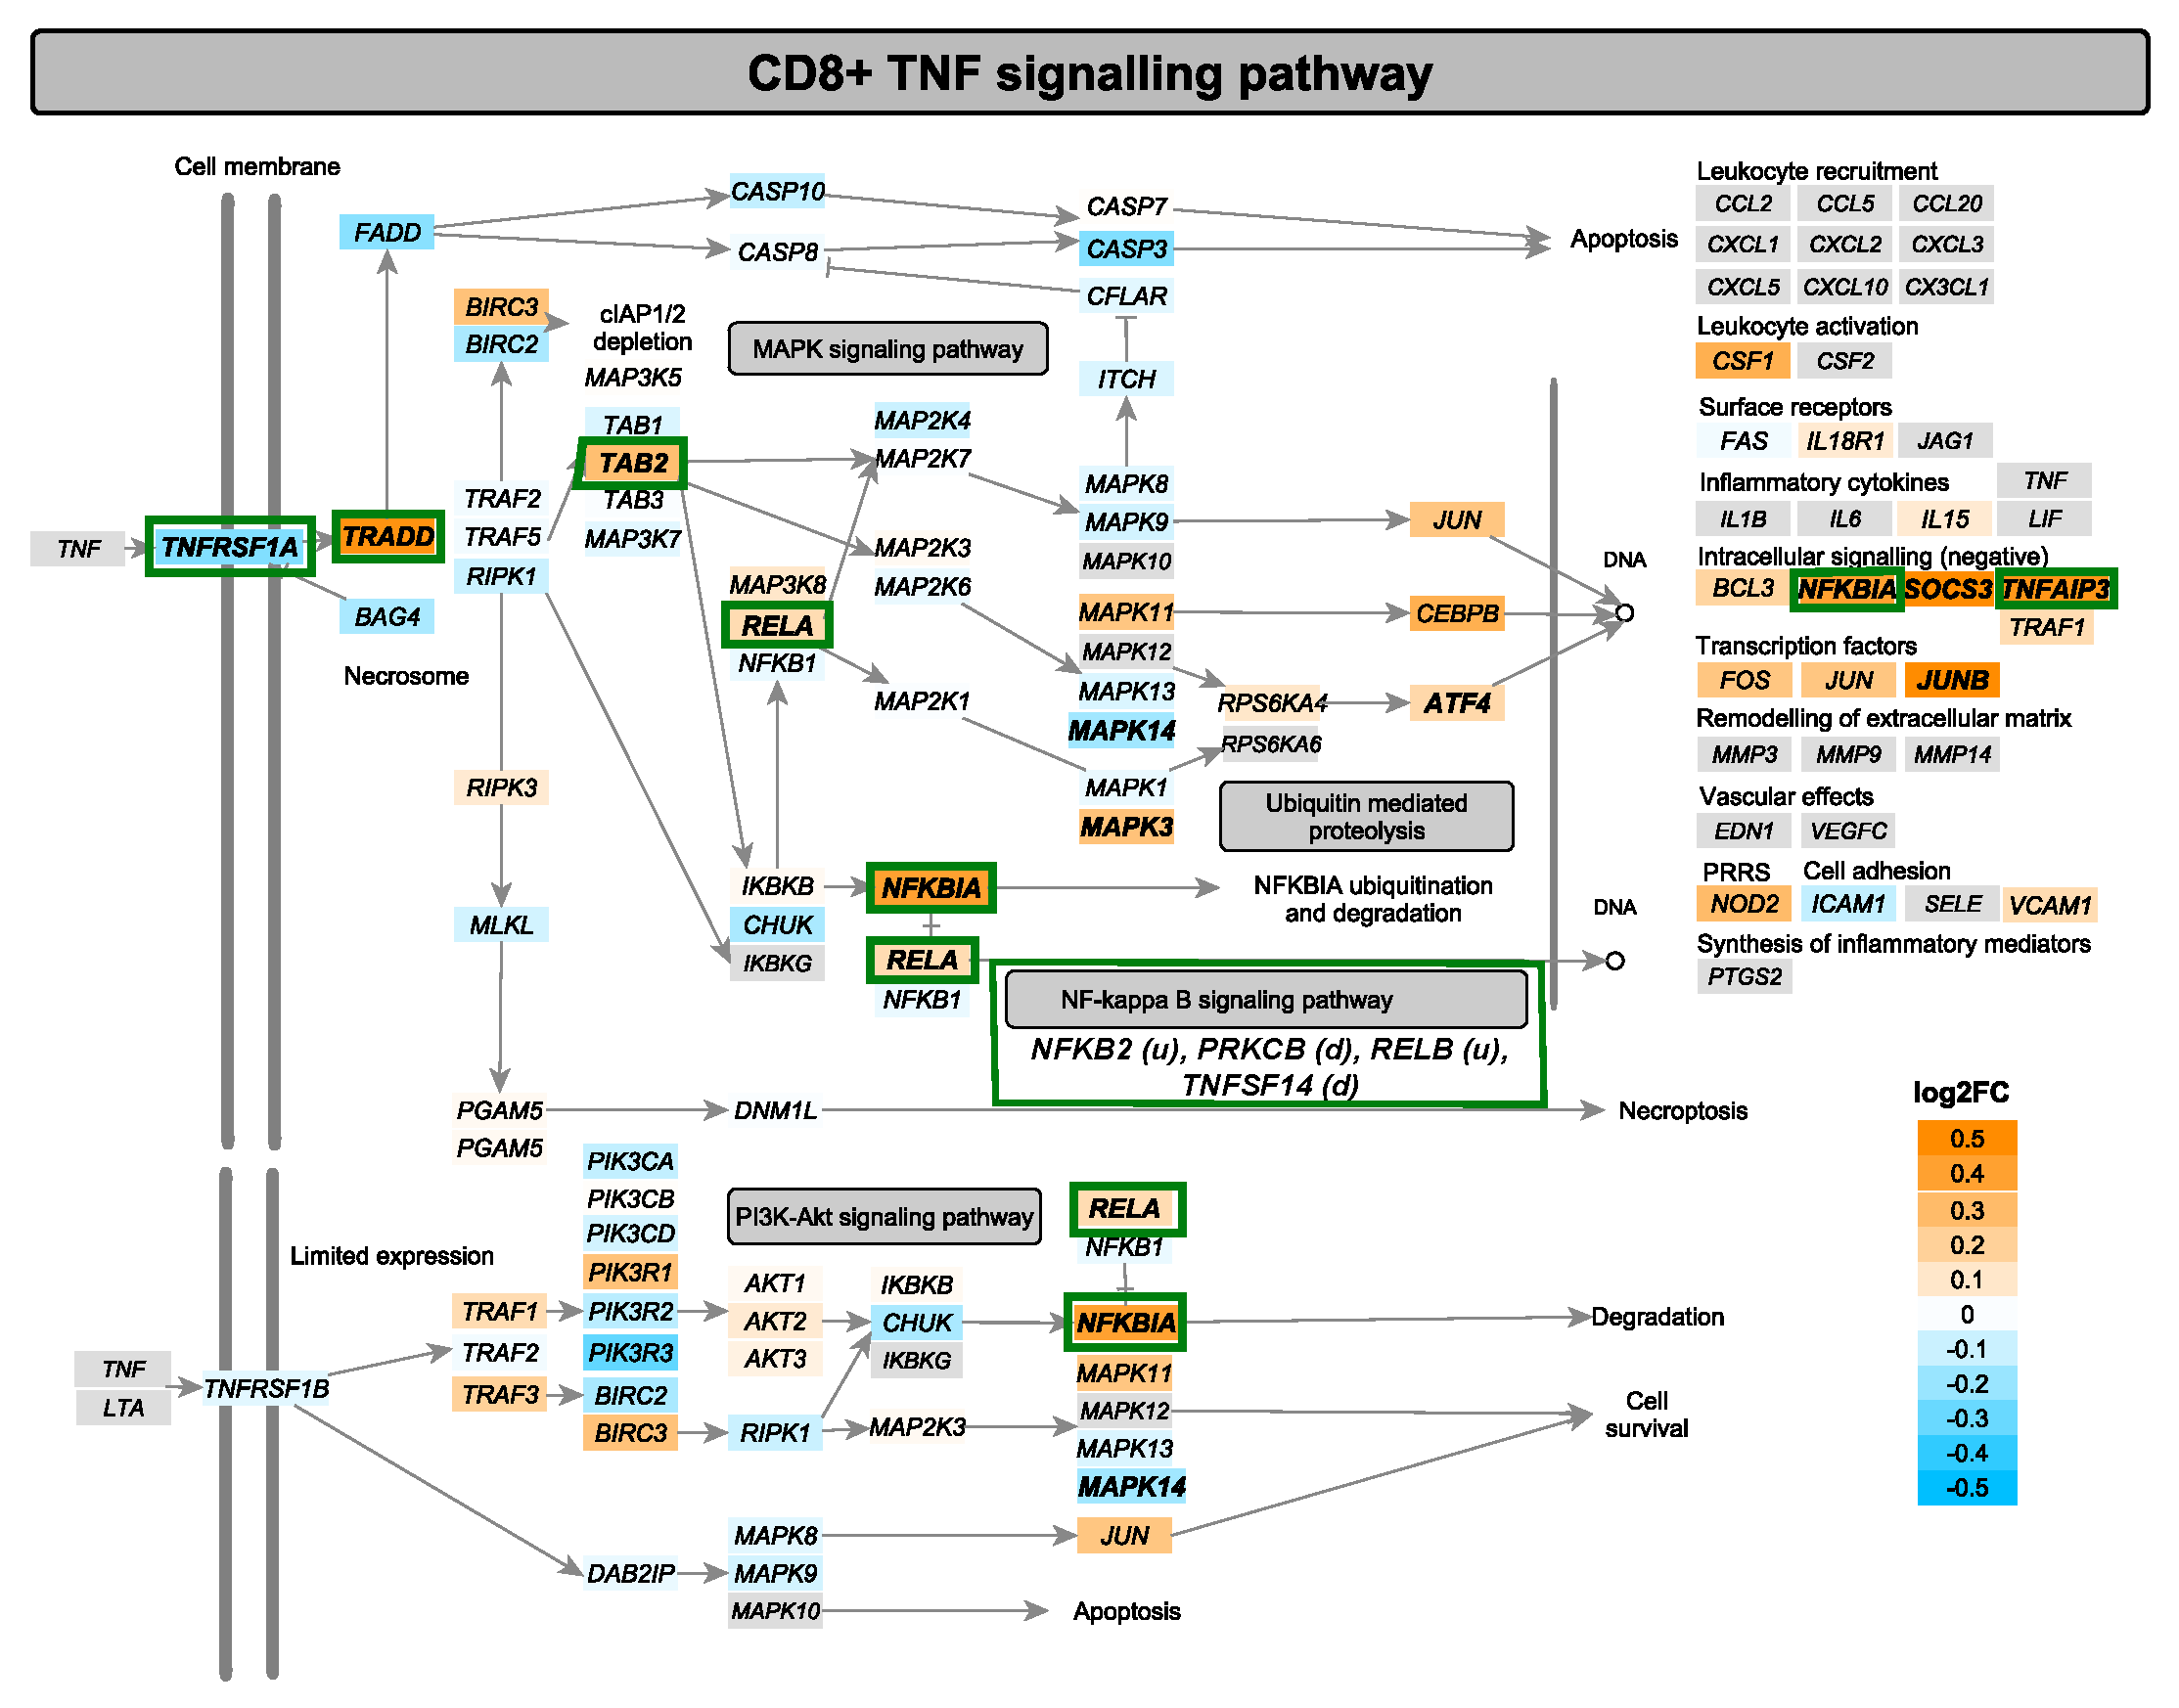
\includegraphics[width=\textwidth]{./Results2/pdfs/PS_CTL_CD8_all_TNF_pathway}
\caption{\textbf{}}
% The percentage sign indicated that the other subfig goes side by side
\end{subfigure}
\begin{subfigure}{0.8 \textwidth}
\centering
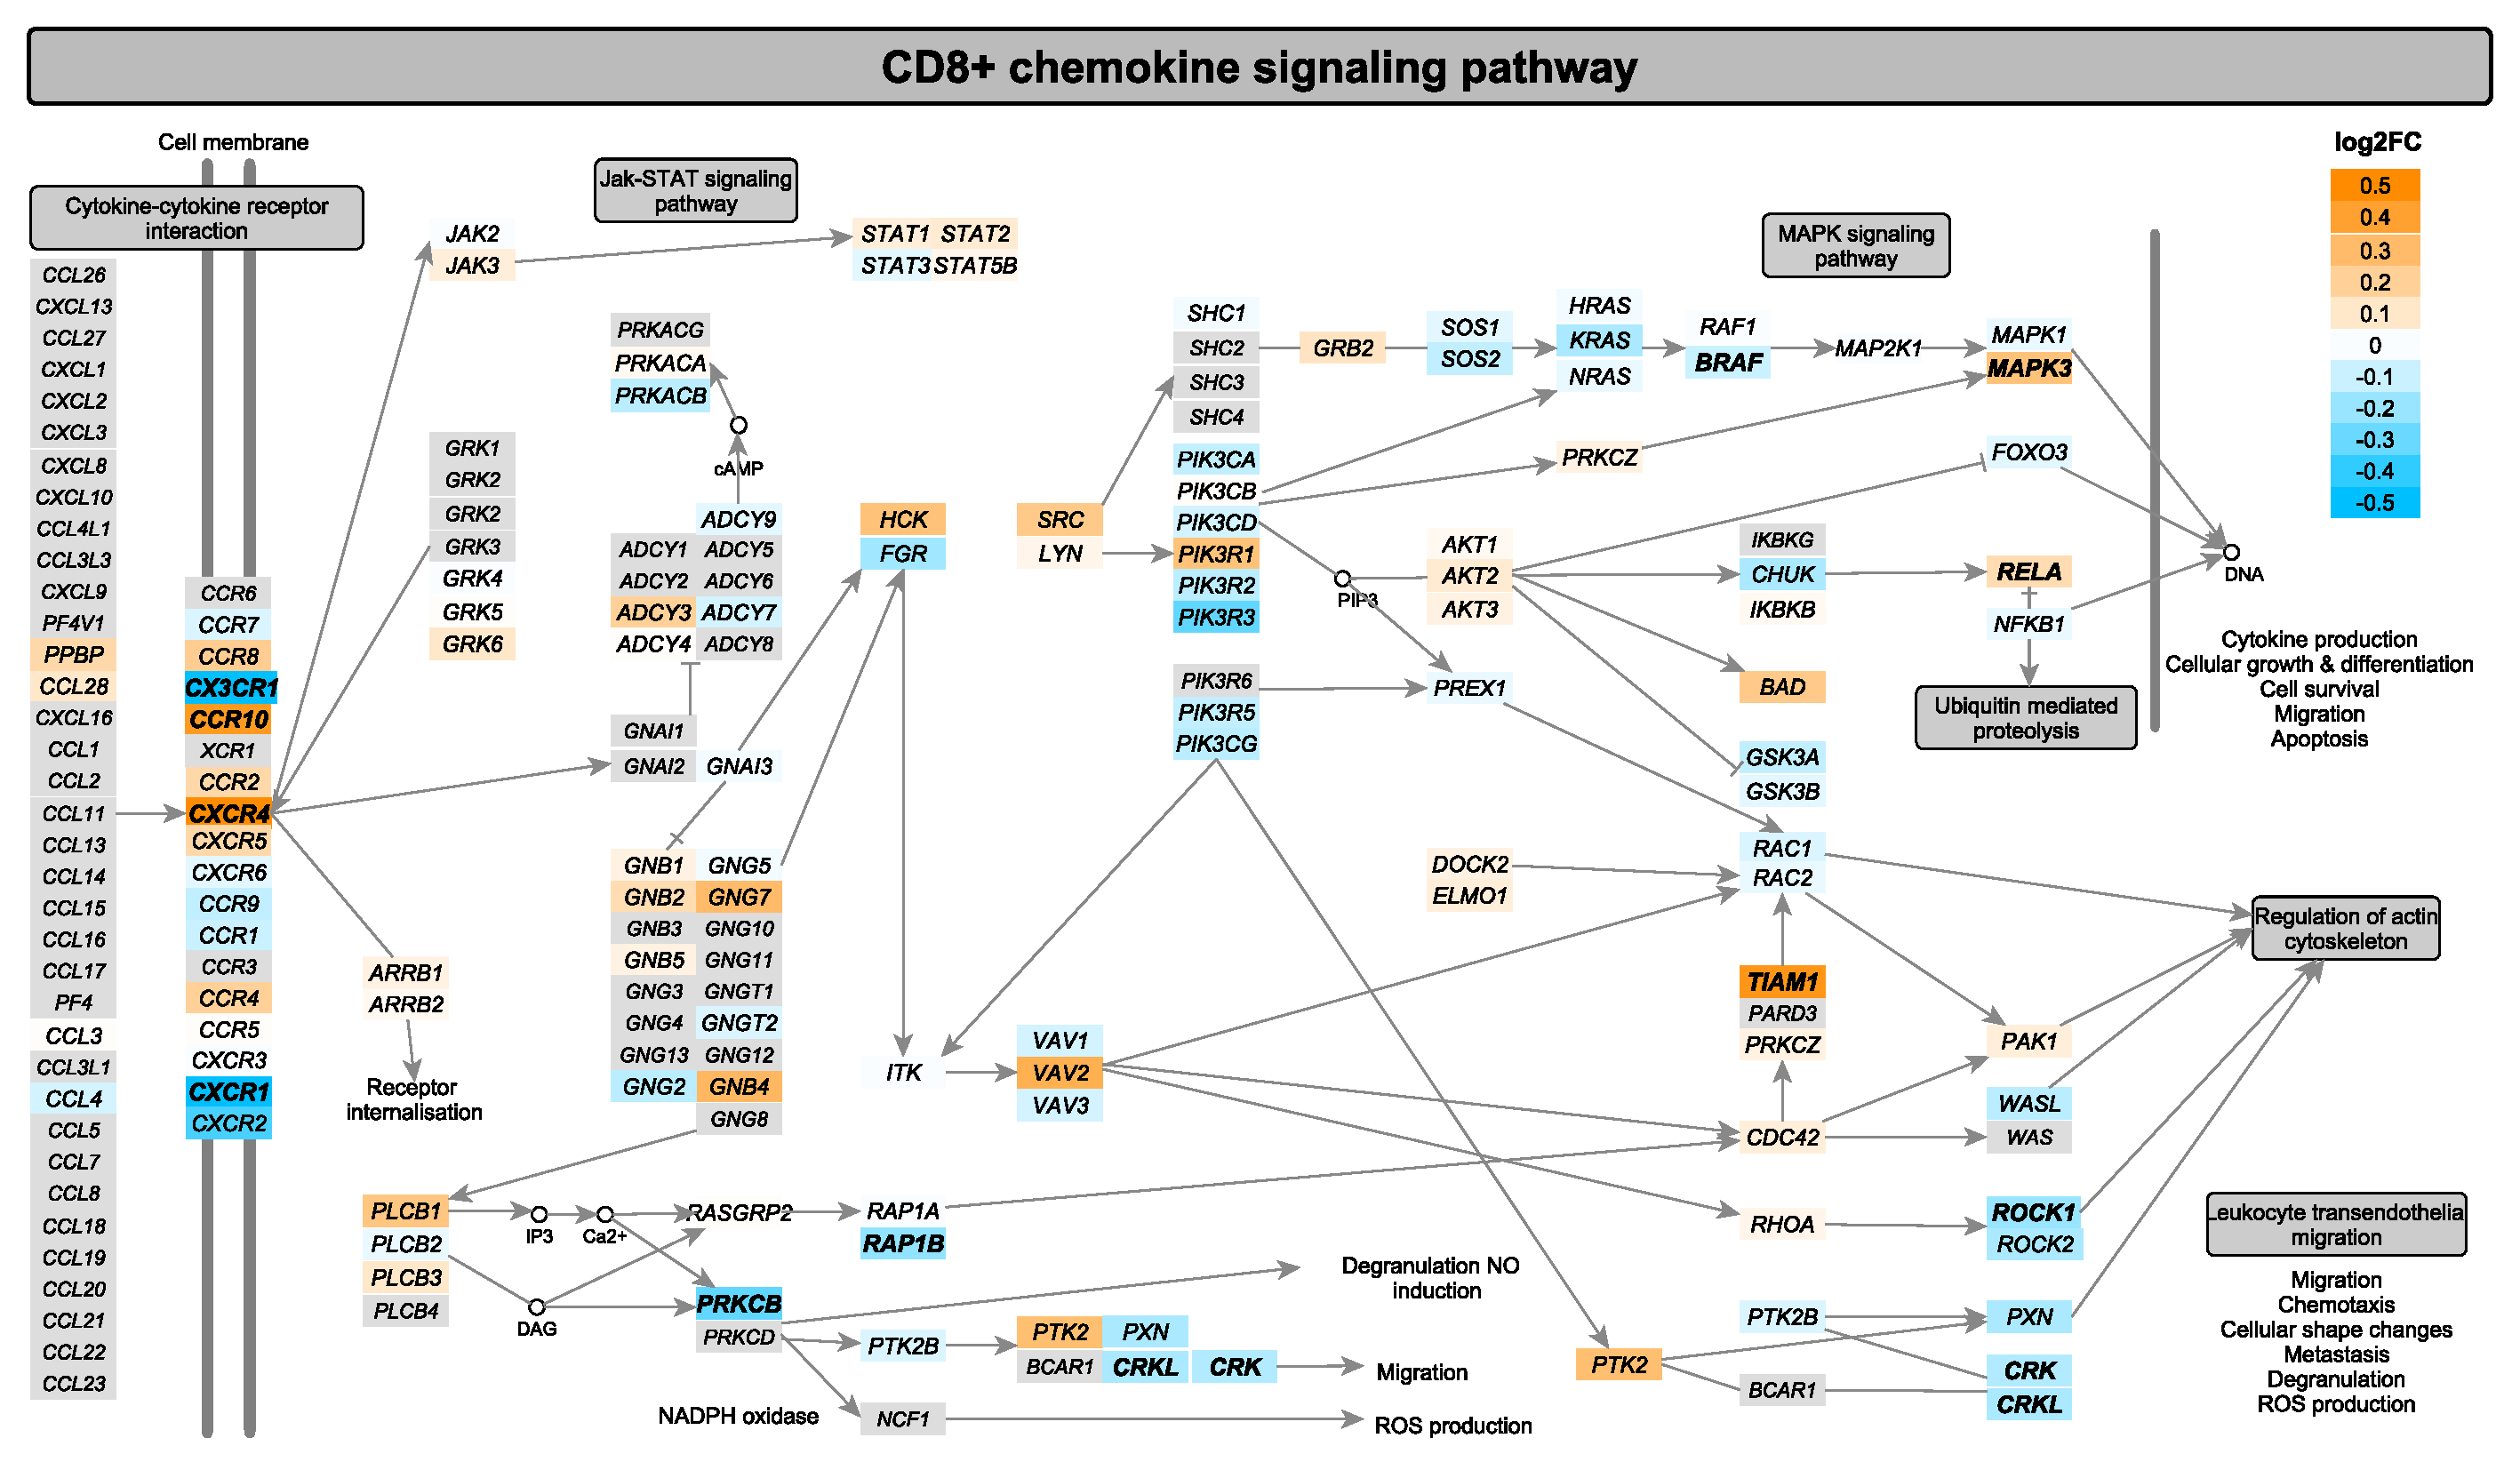
\includegraphics[width=\textwidth]{./Results2/pdfs/PS_CTL_CD8_all_chemokine_pathway}
\caption{\textbf{}}
\end{subfigure}
\caption[Mapping of the DEGs identified in CD8$^+$ cells between psoriasis patients and healthy controls onto the TNF-$\alpha$ and the chemokine signalling pathways.]{\textbf{Mapping of the DEGs identified in CD8$^+$ cells between psoriasis patients and healthy controls onto the TNF-$\alpha$ and the chemokine signalling pathways.} The a) TNF-$\alpha$ and b) chemokine pathways were sourced from KEGG, manually curated in a way that all member genes are maximised visually and then automatically color-coded by the log$_2$FC expression between psoriasis patients and healthy controls CD8$^+$ cells isolated from PB. Significant DEGs (FDR$<$0.05) are highlighted in bold. In a), members of the TNF-$\alpha$ pathway shared with the NF-$\kappa$B are highlighted with a green box. Additional members of the NF-$\kappa$B pathway differentially regulated in CD8$^+$ cells have also been indicated in brackets. Enrichment for a) and b) was identified by using only the CD8$^+$ DEGs (FDR$<$0.05).}
\label{figure:RNAseq_PS_CTL_CD8_TNF_and_chemokine_pathway_modified}
\end{figure}





Other genes with a prominent pro-inflammatory role also appeared to be down-regulated in the NF-$\kappa$B or TNF signalling pathways, such as the activating transcription factor 2 (\textit{ATF2}) and 4 (\textit{ATF4}) members of the TNF signalling cascade and the protein kinase C beta\textit{PRKCB} from the NF-$\kappa$B and chemokine signalling pathways. In contrast, up-regulation of pro-inflammatory genes members of these two pathways were also found. For example JunB proto-oncogene (\textit{JUNB}) coding for one of the subunits of the TF AP-1 and three of the NF-$\kappa$B subunits including \textit{RELA}, \textit{RELB} and \textit{NFKB2}. Particularly, AP-1 undergoes activation following growth factors, cytokines, chemokines, hormones and multiple environmental stresses and acts as a negative regulator of cell proliferation and IL-6 production \parencite{Schonthaler2011}.

Regarding dysregulation of chemokines, a mix of up-regulation and down-regulation of members of this pathway was found in CD8$^+$ cells from psoriasis patients when compared to healthy controls (Figure \ref{figure:RNAseq_PS_CTL_CD8_TNF_and_chemokine_pathway_modified} b). One of the most relevant dysregulated cytokine genes was \textit{CCR10}, the receptor for the chemotactic skin-associated chemokine CCL27. In this data, tCD8$^+$ cells but not tCD4$^+$ cells from psoriasis patients presented up-regulated expression of the \textit{CCR10}. Other up-regulated chemokine receptors in tCD8$^+$ circulating psoriatic cells included \textit{CXCR4} gene, the receptor for the chemokine SDF-1, highly expressed in skin \parencite{Zgraggen2014}. Of note, none of the genes coding for well-known psoriasis drug target genes, including TNF-$\alpha$, IL-17 and IL-6, appeared to be up-regulated in any of the four cells types from psoriasis patients compared to healthy controls.


%Some studies have demonstrated an increased of CCR10$^+$ infiltrated T lymphocytes in psoriasis \parencite{Homey2002}. In circulation, expression of CCR10 is restricted to the a subset of circulating mCD4$^+$ and mCD8$^+$ T cells expressing the cutaneous lymphocyte-associated antigen (CLA), which are preferentially recruited to cutaneous sites of inflammation where KCs express CCL27 \parencite{Hudak2002}. A study in psoriasis circulating cells revealed a correlation between the frequency of CTLA$^+$ CD8$^+$ cells and disease severity measured by PASI score \parencite{Sigmundsd\'{o}ttir2001}. Other up-regulated chemokine receptors in CD8$^+$ circulating psoriatic cells included \textit{CXCR4} gene (receptor for CXCL12) for which ?conflicting findings have been reported about its role in skin inflammation and psoriasis \parencite{Zgraggen2014,Takekoshi2013}.

%TNF:
% ATF4 https://www.tandfonline.com/doi/full/10.1080/15548627.2016.1156823
%JUNB up in psoriasis https://www.jidonline.org/article/S0022-202X(15)32827-X/fulltext;https://www.ncbi.nlm.nih.gov/pubmed/15377346
%PKCB https://www.ncbi.nlm.nih.gov/pmc/articles/PMC5594653/


\subsection{RNA-seq in epidermis from psoriasis patients}

\subsubsection{Data processing and quality control}
For the three paired uninvolved-lesional samples (Table \ref{tab:Psoriasis_controls_datasets_per_sample}), all presented a mapping rate greater than 80\%, with the rate moderately greater in the lesional compared to the uninvolved samples in all three patients (Figure \ref{RNAseq_PS_uninvolved_lesional_psoriasis_skin_mapping_and_PCA} a). The number of reads after filtering that were mapped to Ensembl genes ranged between 29.5 and 33.2 million in PS1011 uninvolved and PS1011 lesional, respectively (Figure \ref{figure:RNAseq_PS_uninvolved_lesional_psoriasis_skin_mapping_and_PCA} b). Similarly to the mapping rate, the final number of reads mapping to genes was greater in the lesional samples compared to the controls.


\begin{figure}[htbp]
\centering
\begin{subfigure}{0.45\textwidth}
\centering
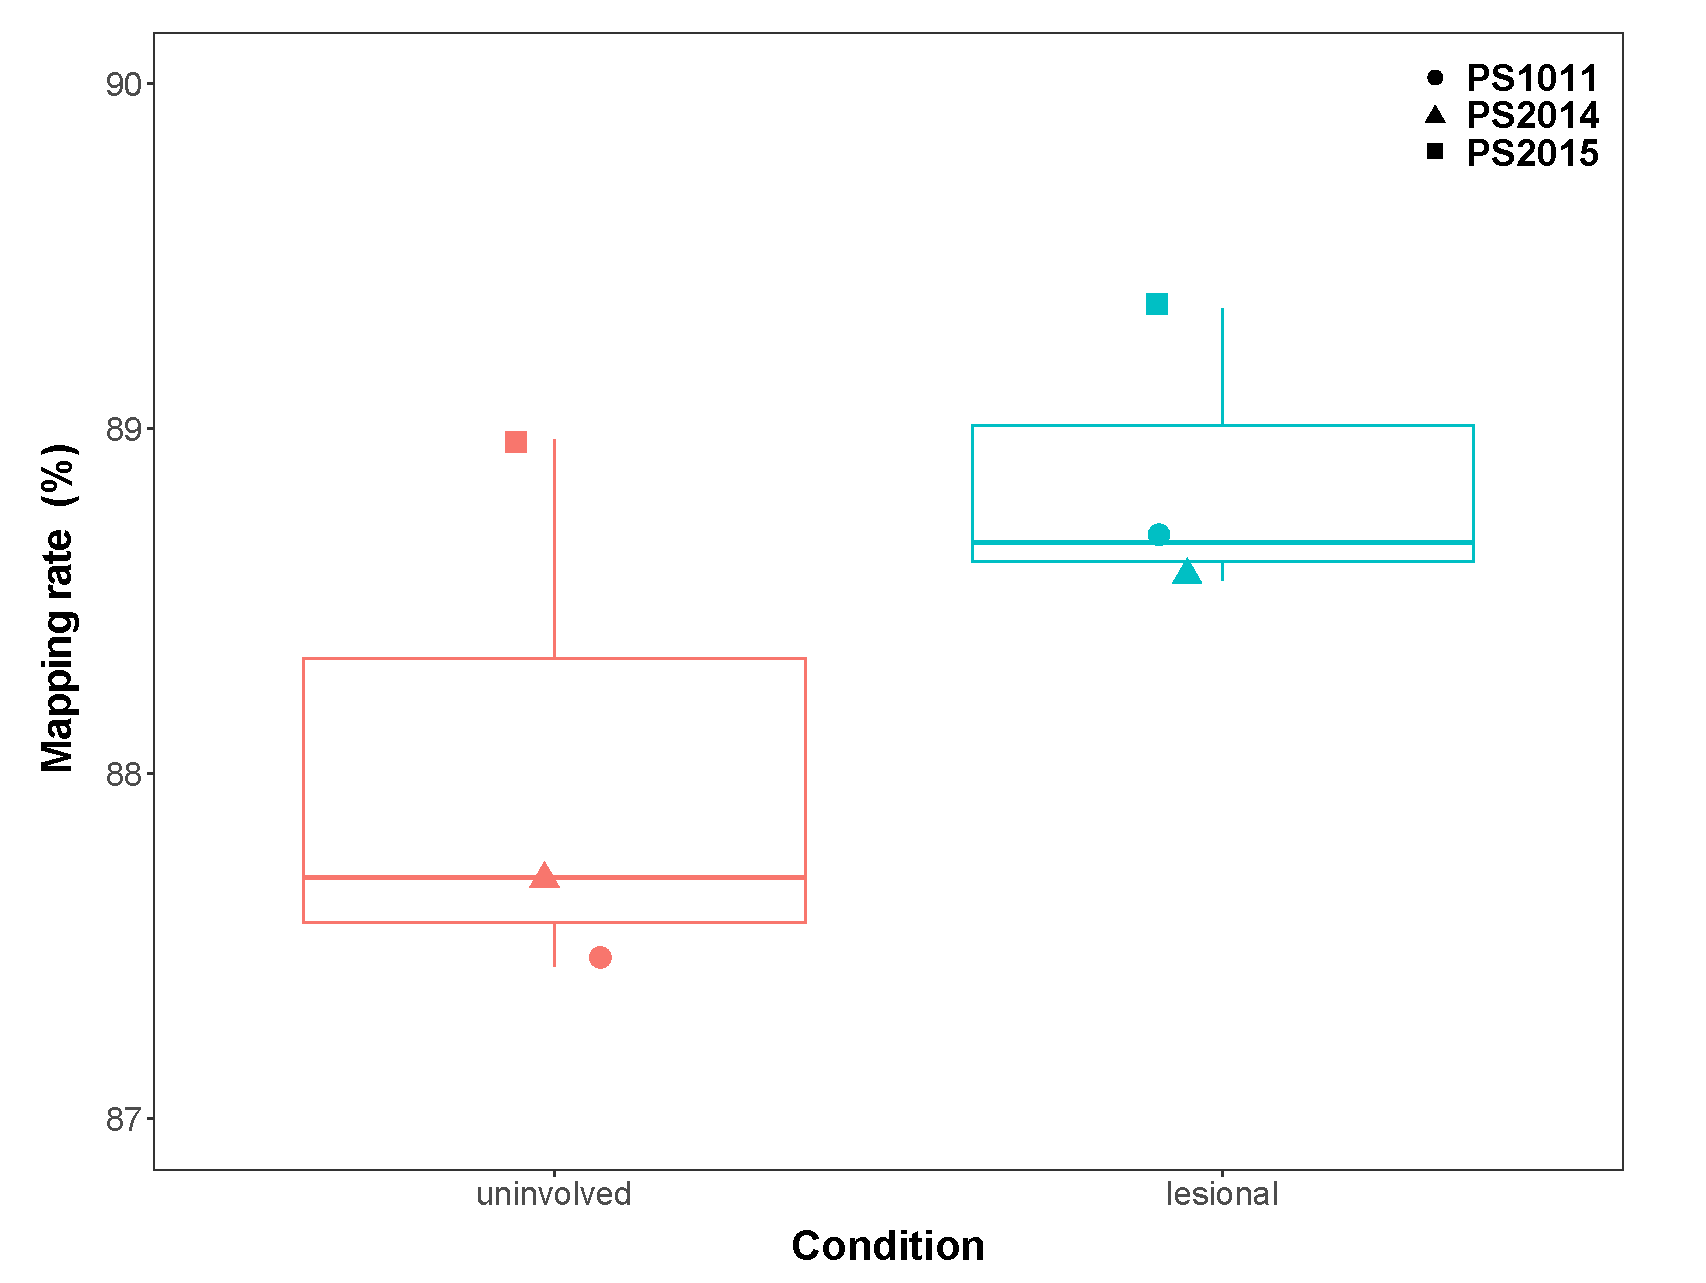
\includegraphics[width=\textwidth]{./Results2/pdfs/PS_lesional_uninvolved_RNAseq_uniquely_mapped_reads_percent_cell_type_and_batch_boxplots}
\caption{\textbf{}}
% The percentage sign indicated that the other subfig goes side by side
\end{subfigure}%
\begin{subfigure}{0.45\textwidth}
\centering
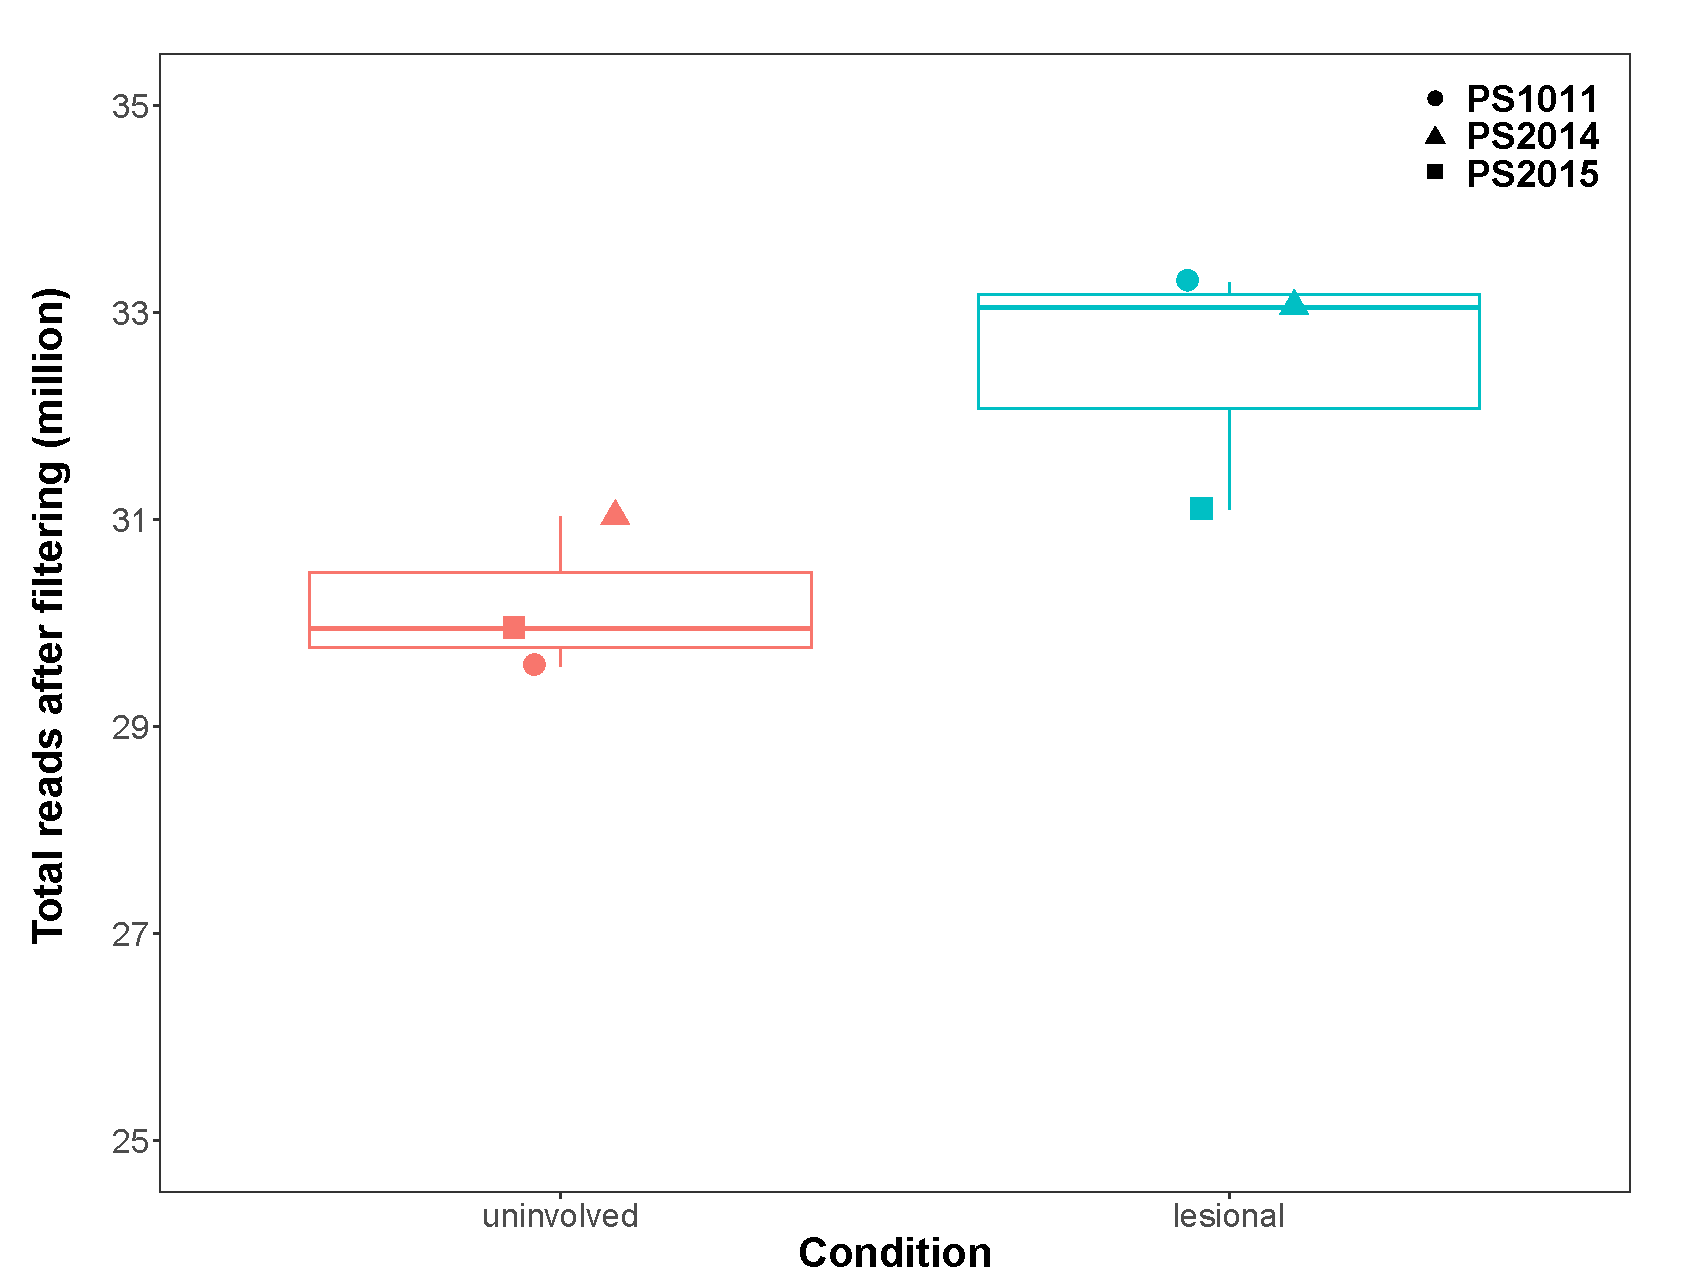
\includegraphics[width=\textwidth]{./Results2/pdfs/PS_lesional_uninvolved_RNAseq_total_reads_per_cell_type_and_batch}
\caption{\textbf{}}
\end{subfigure} \\
\begin{subfigure}{0.4\textwidth}
\centering
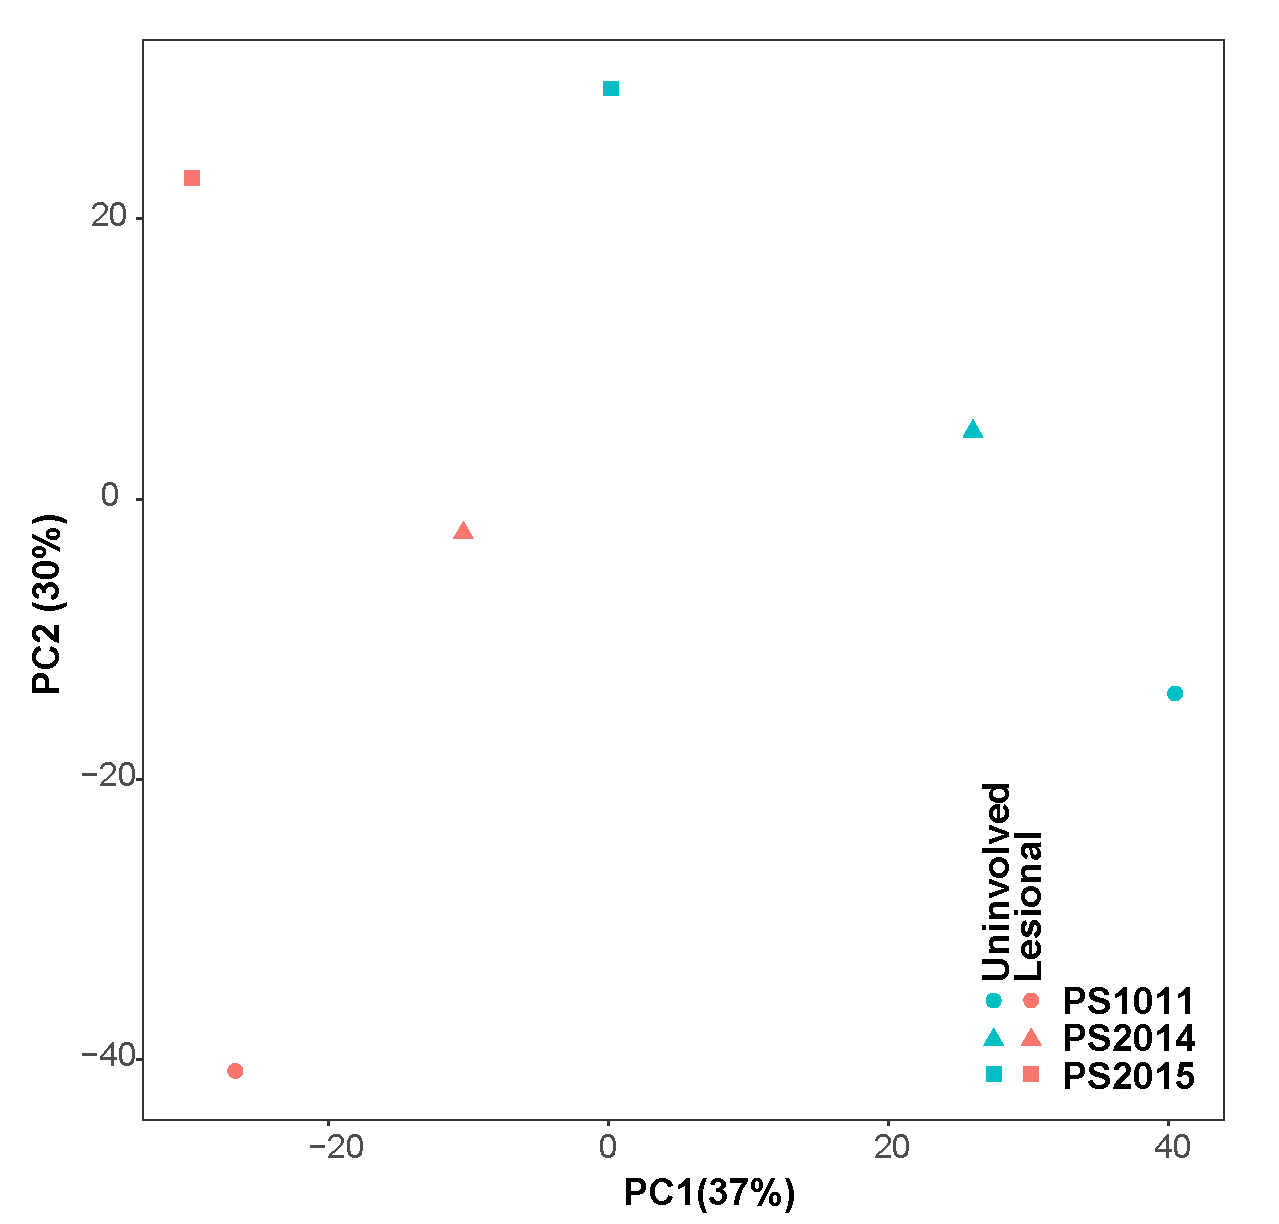
\includegraphics[width=\textwidth]{./Results2/pdfs/PS_lesional_uninvolved_varied_PCA1and2_plot}
\caption{\textbf{}} % to add text to the figure name
\end{subfigure}%
\caption[Mapping quality control and PCA analysis for the RNA-seq data in the uninvolved and lesional epidermis from psoriasis patients.]{\textbf{Mapping quality control and PCA analysis for the RNA-seq data in the uninvolved and lesional epidermis from psoriasis patients.} a) Mapping rate calculated as the proportion of sequencing reads mapping uniquely to a particular region of the genome. b) The total number of reads mapping to an Ensembl feature (including protein coding genes and lncRNAs) after removing the non-uniquely mapped and duplicated reads. c) First and second component of the PCA analysis performed on the normalised number of reads mapping to the Ensmbl list of mRNAs and lncRNAs detected in this study. Dots colour corresponds to condition (lesional or uninvolved) and shape refers to the patient ID.}
\label{figure:RNAseq_PS_uninvolved_lesional_psoriasis_skin_mapping_and_PCA}
\end{figure} 

PCA analysis using the normalised number of reads mapping to the genes after filtering (see Chapter \ref{ch:Mat}) revealed separation of the lesional samples from the uninvolved by the first PC, which explained 37\% of the variance (Figure \ref{figure:RNAseq_PS_uninvolved_lesional_psoriasis_skin_mapping_and_PCA} c). The second PC explained 30\% of the variance and correlated with the patient ID. Overall, PCA analysis revealed substantial variation between the lesional and uninvolved samples and biological variability across individuals, for which the paired design in the DGE analysis accounted.  


\subsubsection{Summary of the DGE results}

DGE analysis revealed a total of 1,227 (FDR$<$0.05) and 702 (FDR$<$0.01) genes dysregulated between the uninvolved and lesional epidermis skin biopsies, including mRNAs and lncRNAs (Table \ref{RNAseq_PS_lesional_uninvolved_DGE_results}). Amongst the 1,227 DEGs, a similar proportion of genes up- (559 genes) and down-regulated (629) in lesional skin when compared to uninvolved were identified (Figure \ref{figure:Skin_DGE_volcano_plot}) and 46 were annotated as lncRNAs (Table \ref{RNAseq_PS_lesional_uninvolved_DGE_results}). The magnitude in the changes of gene expression between lesional and uninvolved skin were notably larger when compared to the changes in expression from analysis in circulating immune cells, with 874 out of 1,227 genes showing FC>1.5.  



\begin{figure}[htbp]
\centering
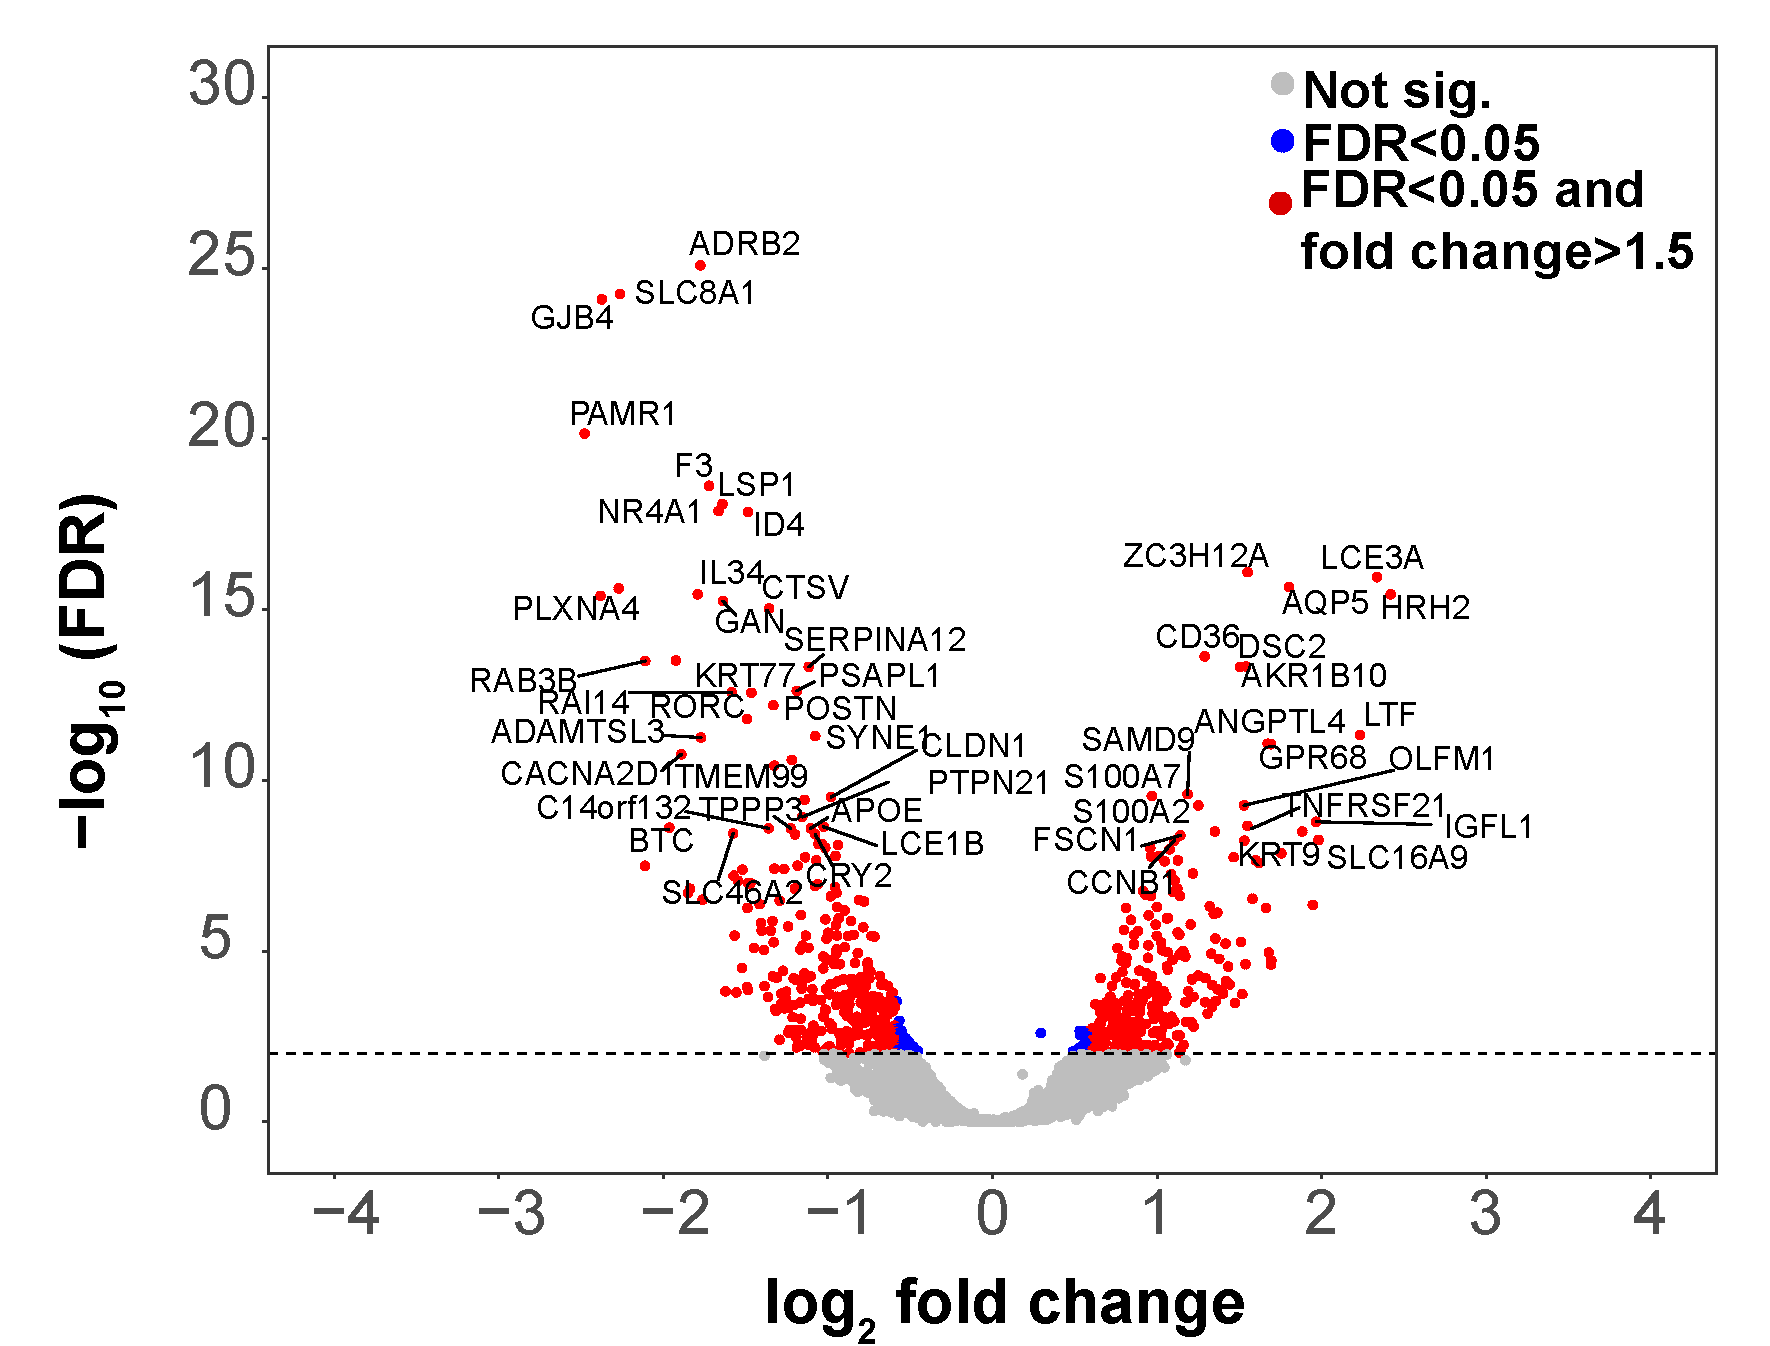
\includegraphics[width=0.5\textwidth]{./Results2/pdfs/RNA_PS_lesional_uninvolved_volcano_plot}
\caption[Magnitude and significance of the gene expression changes between matched lesional and uninvolved epidermal biopsies from three psoriasis patients.]{\textbf{Magnitude and significance of the gene expression changes between matched lesional and uninvolved epidermal biopsies from three psoriasis patients.} The volcano plot represents for each gene the significance (-log$_{10}FDR$) of the log$_2$(FC) in expression for that gene in the lesional skin group with reference to the uninvolved skin. Significant DEGs (FDR$<$0.05) in blue for FC $<$1.5 and red for FC $>$1.5. The volcano plot includes mRNAs and lncRNAs species.}
\label{figure:Skin_DGE_volcano_plot}
\end{figure}

Amongst the DEGs between the uninvolved and lesional skin, five genes (FDR$<$0.05) overlapped with putative GWAS genes (Table \ref{RNAseq_PS_lesional_uninvolved_DGE_results}). \textit{IFIH1}, \textit{NOS2}, \textit{LCE3D} and \textit{STAT3} were up-regulated in lesional compared to uninvolved skin, whereas \textit{TNFAIP3} showed the opposite behavior.

%\textit{IFIH1}, \textit{NOS2}, \textit{LCE3D} and \textit{STAT3} were also found to be up-regulated in lesional compared to uninvolved skin biopsies from psoriasis patients in \parencite{Tsoi2015}. In contrast, \textit{TFNAIP3} was found to be up-regulated in \parencite{Jabbari2011}, opposite to our finding.


\begin{table}[htbp]
%\setlength{\tabcolsep}{20pt} only to stretch the columns if you want
%\renewcommand{\arraystretch}{1.5}
\centering
\begin{tabular}{@{} c c c c}
\toprule
\textbf{FDR threshold}   & \textbf{mRNA}   & \textbf{lncRNA}  & \textbf{Overlap with}\\
                         &                 &                  & \textbf{GWAS genes}\\
\midrule
\midrule
0.05                     & 1181            & 46               &  up(\textit{IFIH1}, \textit{NOS2}, \textit{STAT3},\\ 
                         &                 &                  &  \textit{LCE3D}), down(\textit{TNFAIP3}) \\
0.01                     &  677            & 25               &  \textit{NOS2}, \textit{STAT3},\textit{TNFAIP3},\textit{LCE3D} \\
\bottomrule 
\end{tabular}
\medskip %gap
\caption[Summary results of the DGE analysis between uninvolved and lesional psoriatic epidermal biopsies.]{\textbf{Summary results of the DGE analysis between uninvolved and lesional psoriatic epidermal biopsies.} Number of differentially expressed mRNAs and lncRNAs are reported for two threshold of significance (FDR$<$0.05 and FDR$<$0.01). The DEGs overlapping putative psoriasis GWAS genes and the directionality in the change of expression are also specified.}
\label{tab:RNAseq_PS_lesional_uninvolved_DGE_results}
\end{table}
\bigskip %bigger spac




\subsubsection{Overall comparison with other skin transcriptomic studies}

As detailed in Chapter \ref{ch:Mat}, the approach to study DGE in skin is different from most of the previously published studies using whole punch biopsies to compare lesional and uninvolved skin from psoriasis patients. During the course of this project a study published by Tervaniemi and colleagues also aimed to characterise the transcriptional profiles of the epidermis from psoriasis patients’ lesional and uninvolved skin in a more elegant way than the previous studies using full thickness skin biopsies \parencite{Tervaniemi2016}. %As previously detailed, Tevaniemi \textit{et al.} had a bigger sample size (six psoriasis patients) compared to this study (three psoriasis patients) and also included nine control epidermis biopsies. 
In order to explore the similarities between the two studies, a comparison for the DEGs identified between lesional and uninvolved matched samples was conducted. 

Tervaniemi reported a total of 2,589 DEGs passing their filtering criteria (FC$<$0.75 or FC$>$1.5 and FDR$<$0.05) and showing overall a larger number of differentially expressed genes between the two types of biopsies compared this study. The number of genes up-regulated in lesional epidermis compared to uninvolved (2,330) was larger than the number of down-regulated targets (261), contrasting to the in-house results where similar numbers of up- and down-regulated genes were found (Table \ref{RNAseq_PS_lesional_uninvolved_DGE_results} and Figure \ref{figure:Skin_venn_diagrams_comparison_other_studies} bottom panel). Regarding overlap, a total of 359 out of the 1,227 DEGs (29.25\%) identified by the in-house study were shared with the Tervaniemi results, of which 239 and 75 were up- and down-regulated, respectively. Amongst the up-regulated genes in both studies TFs such as \textit{STAT1}, genes from the \textit{S100} family (e.g \textit{S100A9} and \textit{S100A12}) and genes nearby psoriasis GWAS loci such as \textit{STAT3} and \textit{IFIH1}. The direction of change in 45 out of the 359 shared genes appeared to be opposite across the two datasets. For example, \textit{SERPINB2} gene, a serine protease inhibitor of the serpin superfamily, presented down-regulation in the in-house data and up-regulation in the Tervaniemi results. Interestingly, a study demonstrated a defective stratum corneum in \textit{SERPINB2} deficient mice as well as greater susceptibility to developing inflammatory lesions upon chemically induced atopic dermatitis compared to wild type controls \parencite{Schroder2016}. 


%The direction of change in 45 out of the 359 shared genes appeared to be opposite across the two datasets. For example, \textit{SERPINB2} gene, a serine protease inhibitor of the serpin superfamily,presented down-regulation in the in-house data and cultured lesional KCs from Swindell \textit{et al.}, 2017 in contrast to the up-regulation in the Tervaniemi results. Interestingly, a study demonstrated a defective stratum corneum in \textit{SERPINB2} deficient mice as well as greater susceptibility to developing inflammatory lesions upon chemically induced atopic dermatitis compared to wild type controls \parencite{Schroder2016}.   


\begin{figure}[htbp]
\centering
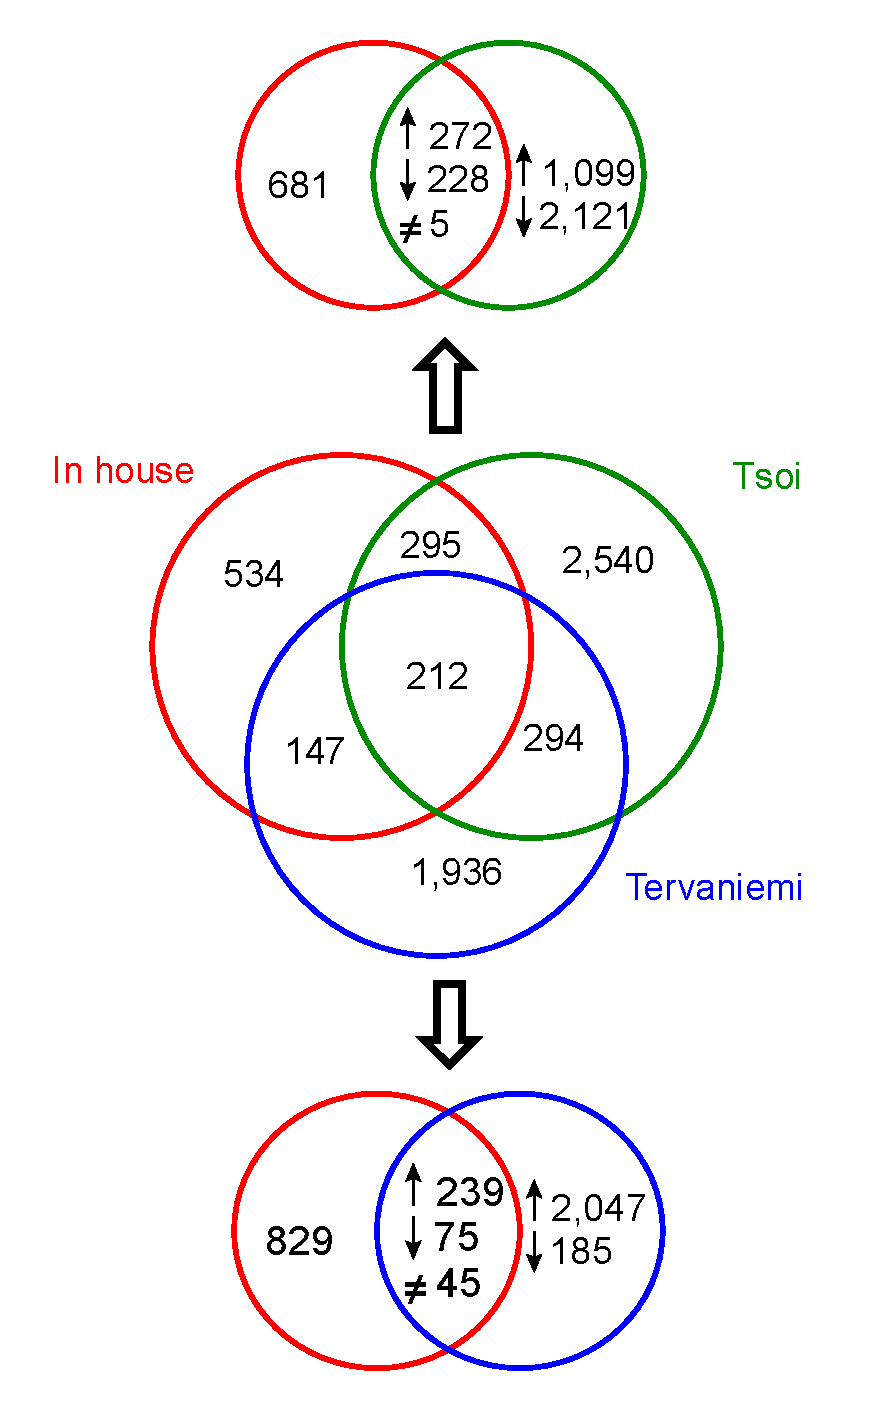
\includegraphics[width=0.5\textwidth]{./Results2/pdfs/skin_transcriptomics_venn_diagrams}
\caption[Overlap of the significantly differentially expressed genes between lesional and uninvolved epidermal sheets, split epidermis and whole skin biopsies.]{\textbf{Overlap of the significantly differentially expressed genes between lesional and uninvolved epidermal sheets, split epidermis and full-thickness skin biopsies.} The central venn diagram illustrated the DEGs overlapping between this study (in house), Tervaniemi \textit{et al.}, 2016 split epidermis biopsies and Tsoi \textit{et al.},2015 full thickness skin biopsies. Overlap is considered regardless the direction of the change. Two additional venn diagrams provide more detail about the total overlap and directionality in the change of gene expression between the in-house data and the Tsoi \textit{et al.} (top) or Tervaniemi \textit{et al.} (bottom).}
\label{figure:Skin_venn_diagrams_comparison_other_studies}
\end{figure}



In addition to the Tervaniemi study, our results were further contrasted to one of the most recent comprehensive RNA-seq studies comparing lesional and uninvolved full thickness skin biopsies from psoriasis patients \parencite{Tsoi2015}. Out of the 3,725 DEGs reported by Tsoi and colleagues, 507 genes were shared between the two studies (41\% of the in-house DEGs) and 24 corresponded to dysregulated lncRNAs. Out of the 507 commonly dysregulated genes in the two datasets, 272 were up-regulated, 228 down-regulated and 7 presented opposite direction of change (Figure \ref{figure:Skin_venn_diagrams_comparison_other_studies} top panel). Some of the genes found dysregulated in the same direction between the in-house and Tervaniemi's stuy were also consistently dysregulated in Tsoi analysis, including \textit{STAT1}, \textit{S100} and the GWAS genes \textit{STAT3} and \textit{IFIH1}. Moreover, the GWAS gene \textit{NOS2} was also a shared up-regulated hit with Tsoi's data, which was noy fooud to be dysregulated in Tervaniemi's analysis. The genes showing dysregulation in the opposite direction included \textit{ALOX15B},  \textit{ARG2}, \textit{LCE6A},\textit{MGST1}, \textit{PNLIPRP3}, \textit{TLDC1} and \textit{UBL3}. For example, \textit{LCE6A}, a member of the\textit{LCE} family involved in the synthesis of the later cornified envelope layer, was down-regulated in lesional skin in our study, in contrast to the up-regulation found in the Tsoi analysis. Notably, down-regulation of genes from the LCE family, including \textit{LCE1B}, \textit{LCE1F} and \textit{LCE2A}, showed opposite direction of change in both, Tsoi and Tervaniemi's analyses. An study performing qPCR quantification of \textit{LCE} genes from groups 1, 2, 5 and 6 demonstrated increased expression in psoriasis lesional skin, in line with the in-house results \parencite{Bergboer2011}. In contrast to the other genes from the \textit{LCE} family, all three datasets presented up-regulation of the GWAS risk associated gene \textit{LCE3B}. 

Overlap across the three studies only identified 212 DEGs shared by the three datasets. Despite having a the larger sample size, the Tsoi and colleagues study did not capture all the DEGs from the in-house or Tervaniemi (506 overlapping genes, Figure \ref{figure:Skin_venn_diagrams_comparison_other_studies} middle panel) data. This may suggest, amongst other things, some of the DEGs being specific to the type of biopsy used on each approach. 
%Notably, qPCR quantification of \textit{LCE} genes from groups 1, 2, 5 and 6 demonstrated increased expression in psoriasis lesional skin \parencite{Bergboer2011}. 


%Overall, the comparison of our results with these two studies suggested greater similarities with the full skin thickness biopsies from Tsoi \textit{et al.}, 2015 in terms of DEGs overlapping, due to different technical reasons as further detailed in the Discussion. 

\subsubsection{Dysregulated lncRNAs in the psoriatic lesional skin}

In addition to protein coding genes, a total of 46 lncRNAs were also significantly (FDR$<$0.05) differentially expressed between uninvolved and lesional skin in the three psoriasis patients from this study. Out of the 46 differentially regulated lncRNAs, 37 had a functional experimental partner functionally validated according to NPInter database \parencite{Hao2016}. An interesting  example was \textit{H19} which was significantly down-regulated in the lesional skin when compared to uninvolved. \textit{H19} has been described to directly bind miR-130b-3p, which down-regulates Desmoglein 1 (\textit{DSG1}), a gene promoting KC differentiation \parencite{Li2017}. Nevertheless, \textit{DSG1} did not appear as one of the DEGs between lesional and uninvolved skin. %This finding was consistent with Tsoi \textit{et al.}, 2015 and also with results from Li \textit{et al.}, 2014 and ?\textit{et al.}, 2016 where they compared lesional versus normal skin. 

Interestingly, four miRNAs (\textit{MIR146A}, \textit{MIR22HG}, \textit{MIR31HG} and \textit{MIR205HG}) were also captured with the standard library preparation for mRNAs and lncRNAs implemented in our project. The relevance of miR-146a has been already commented in the DGE analysis from circulating immune cells. In lesional skin \textit{MIR146A} was up-regulated when compared to uninvolved skin, consistently with other studies \parencite{Lerman2014, Tsoi2015}, and was also shown to have increased expression when comparing lesional skin versus healthy biopsies \parencite{Li2014}. One of the predicted miR-146a targets by Target Rank software in a study conducted by Jazdzewski and colleagues revealed \textit{NFAT5}, also down-regulated in lesional skin compared to uninvolved in the in-house data, as the 11$^{th}$ most confidently predicted target \parencite{Jazdzewski2009}. Interestingly, a negative correlation (R=-0.981, pval=5.3x10$^{-4}$) between the normalised counts of the two genes was found in the three lesional-uninvolved paired samples (Figure \ref{figure:RNAseq_lesional_uninvolved_miR_correlations} a).
%check if target genes dysregulated https://www.pnas.org/content/106/5/1502
%Moreover, a polymorphism in miR-146a has been associated with psoriasis in a small cohort study and a \textit{MIR146A} knock-out mice with chemical induced psoriasis led to earlier disease onset and amplified epidermal activation \parencite{Srivastava2017}. 


\begin{figure}[htbp]
\centering
\begin{subfigure}{0.45\textwidth}
\centering
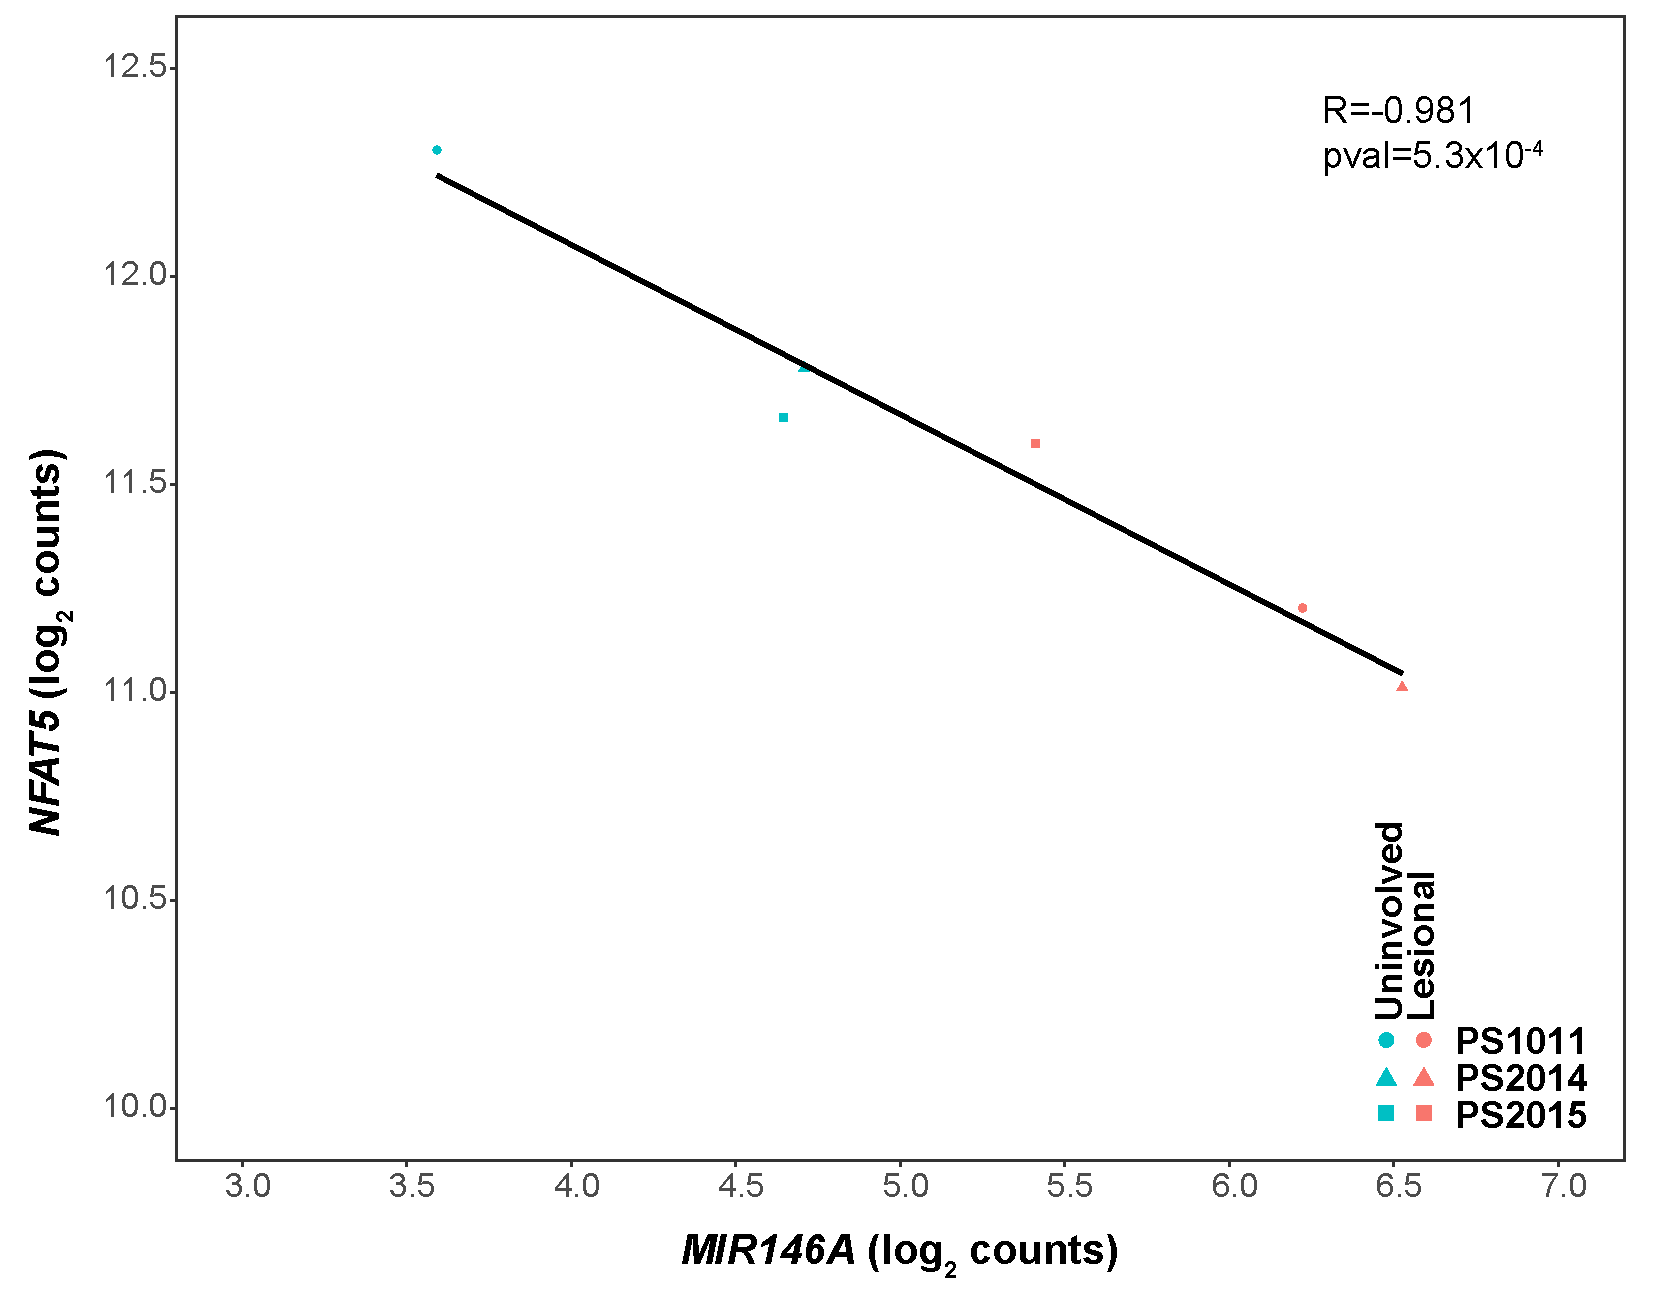
\includegraphics[width=\textwidth]{./Results2/pdfs/Skin_RNAseq_correlation_MIR146A_NFAT5_plot}
\caption{\textbf{}}
% The percentage sign indicated that the other subfig goes side by side
\end{subfigure}%
\begin{subfigure}{0.45 \textwidth}
\centering
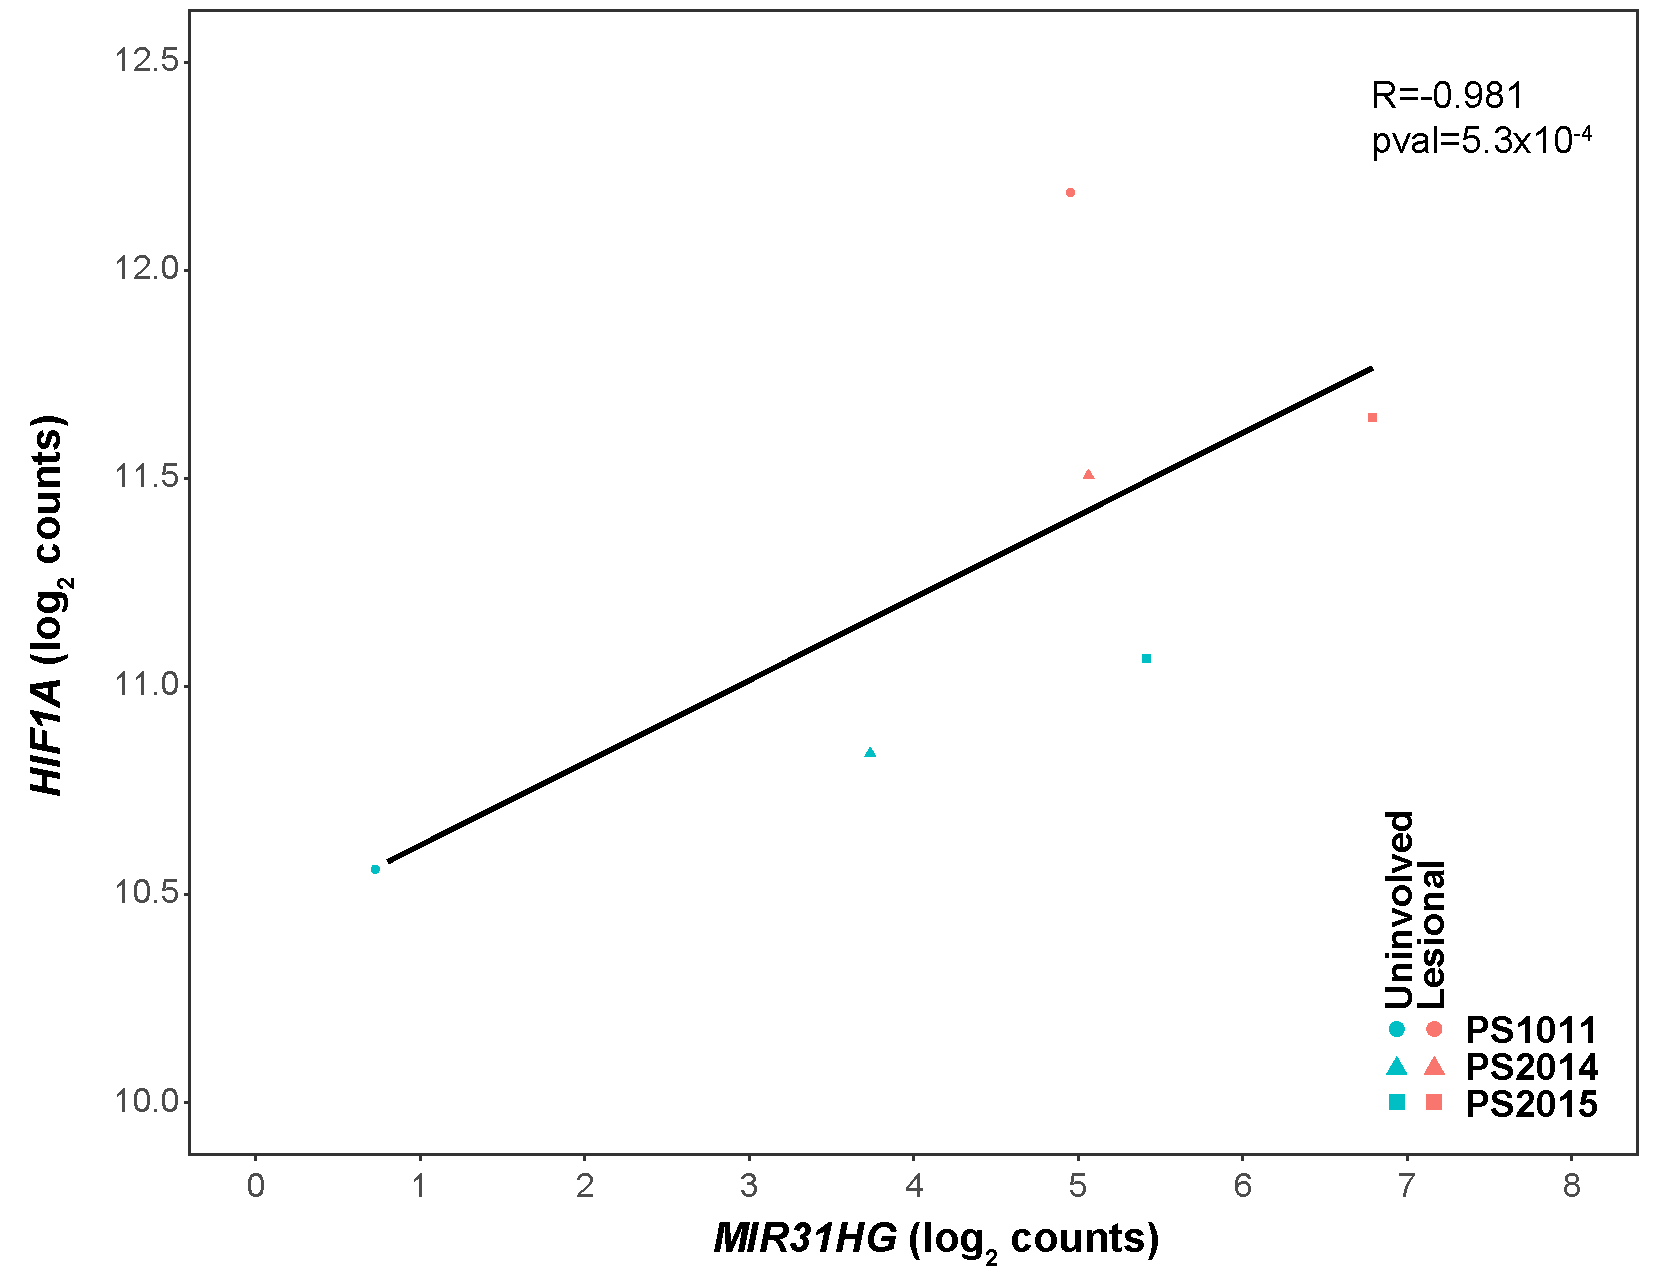
\includegraphics[width=\textwidth]{./Results2/pdfs/Skin_RNAseq_correlation_MIR31HG_HIF1A_plot}
\caption{\textbf{}}
\end{subfigure}
\caption[Correlation in gene expression between two dyregulated miRs in lesional skin and their putative target genes.]{\textbf{Correlation in gene expression between two dyregulated miRs in lesional skin and their putative target genes.} Plots showing the correlation in log$_2$ normalised read counts for a) \textit{MIR146A} and its putative target genes \textit{NFAT5} and b) \textit{MIR31HG} and its putative target genes \textit{HIF-1A}. Pearson correlation values (R) and significance (pval) are included. Each of the dots represents one samples, where colour represents condition (lesional or uninvolved) and shape corresponds to the patient ID.}
\label{figure:RNAseq_lesional_uninvolved_miR_correlations}
\end{figure}



Another relevant finding was the up-regulation of \textit{MIR31HG} in lesional skin, which has also been reported by \parencite{Tsoi2015}. In a study in head and neck carcinoma, \textit{MIR31HG} expression was identified to target \textit{HIF-1A}, inducing up-regulation by an unknown mechanisms. In our data, \textit{HIF-1A} showed up-regulation in lesional skin compared to uninvolved, and a trend for positive correlation (R=0.690, pval=0.12) between normalised counts of this gene and the putative regulator \textit{MIR31HG} was also observed (Figure \ref{figure:RNAseq_lesional_uninvolved_miR_correlations} b).
%Notably, a functional study using the KC immortal cell line HaCaT demonstrated that silencing miR-31hg induces cell cycle arrest and inhibits cell proliferation consistently with two characteristic functions dysregulated in psoriatic KCs \parencite{Gao2018}.
%also role in osteogenesis https://www.ncbi.nlm.nih.gov/pubmed/27334046
%HIF-1 up-regulation https://molecular-cancer.biomedcentral.com/articles/10.1186/s12943-018-0916-8


%\begin{table}[htbp]
%%\setlength{\tabcolsep}{20pt} only to stretch the columns if you want
%%\renewcommand{\arraystretch}{1.5}
%\centering
%\begin{tabular}{@{} c c c}
%\toprule
%\textbf{Transcript class}   & \textbf{Gupta \textit{et al.},}   & \textbf{Li \textit{et al.}}  \\
                            %& \textbf{2016}                     &      \textit{2014}            \\
%\midrule
%\midrule
%mRNA                        & xxx                               & xxxx                \\
%lncRNAs (functionally       & 2 (\textit{H19} (d),              & 7 (\textit{H19} (d), \textit{NEFL} (d), \textit{SCARNA2} (d),\\
%characterised)              & \textit{LINC00302} (u))           & \textit{SCARNA9} (d), \textit{SCARNA10} (d),\textit{UHRF1} (u),\\
                            %&                                   &  \textit{KCNQ1OT1} (d)) \\
%\bottomrule 
%\end{tabular}
%\medskip %gap
%\caption[Summary results of the DGE analysis between uninvolved and lesional psoriatic epidermal biopsies.]{\textbf{}u=up-regulated; d=down-regulated. Directionality for the differentially expressed lncRNA included in this table was concordant with other studies having reported them previously for all of them but \textit{LINC00302} which appeared down-regulated in this data.}
%\label{tab:RNAseq_PS_lesional_uninvolved_overlap_with_other_studies}
%\end{table}
%\bigskip %bigger spac



\subsubsection{Pathway enrichment analysis}

In order to better understand the functional role of the DEGs (FDR$<$0.05) between lesional and uninvolved epidermis from psoriasis patient skin biopsies, pathways enrichment analysis was performed. A considerable number of pathways were significantly enriched (FDR$<$0.005) for DEGs found in our analysis (Table \ref{tab:RNAseq_PS_lesional_uninvolved_pathway_enrichment} and \ref{tab:RNAseq_PS_lesional_uninvolved_additional_pathways}). 


\begin{table}[htbp]
%\setlength{\tabcolsep}{20pt} only to stretch the columns if you want
%\renewcommand{\arraystretch}{1.5}
\centering
\begin{tabular}{@{}c}
\toprule
\textbf{Lesional versus uninvolved epidermis enriched pathways} \\
\midrule
\midrule
IFN-$\alpha$/$\beta$/signalling \\
Peroxisome proliferator-activated receptors (PPAR) signalling \\
NOD-like receptor signaling pathway \\
IL-17 signalling \\
IL2-mediated signalling \\
G protein coupled receptor (GPCR) ligand binding \\
Hypoxia-inducible factor 1 (HIF-1) signalling \\
Cytokine signalling in immune system \\
Cell cycle \\
Apoptosis \\
Arginine and proline metabolism \\
\bottomrule
\end{tabular}
\medskip %gap
\caption[Most relevant pathways enriched for DEGs between lesional and uninvolved epidermis isolated from psoriasis patients skin biopsies.]{\textbf{Most relevant pathways enriched for DEGs between lesional and uninvolved epidermis isolated from psoriasis patients skin biopsies.} Significant pathways for FDR$<$0.005. The analysis was performed using significantly DEGs FDR$<$0.05 and no FC threshold. Enriched pathways had a minimum of ten members overlapping with DEGs.}
\label{tab:RNAseq_PS_lesional_uninvolved_pathway_enrichment}
\end{table}


A number of pathways were related to alterations in cell cycle and metabolic processes, including hypoxia-inducible factor 1 (HIF-1) signalling, arginine and proline metabolism,glycolysis/gluconeogenesis and metabolism of amino acids and derivatives. %Dysregulation  of similar functions have previously also been reported in other studies comparing lesional and uninvolved skin and genome-wide pathway analysis\parencite{Coda2012, Aterido2016, Tervaniemi2016}. 
HIF-I signalling has been found to be up-regulated in psoriasis skin, likely through hypoxia caused by increased cell proliferation rates and epidermal thickening. In this data up-regulation of \textit{HIF1A}, \textit{VEGFA}, \textit{ENO1} and the GWAS gene \textit{NOS2}, amongst others, contributed to the enrichment of this pathway (Figure \ref{figure:PS_lesional_vs_uninvolved_HIF_pathway}). 
%Up-regulated expression of the hypoxia-inducible TFs HIF-1$\alpha$ and HIF-2$\alpha$ has been found in lesional skin and co-related with the increase in \textit{VEGF} transcript levels, a target gene regulated by HIFs that mediates the pathological angiogenesis driving psoriasis \parencite{Rosenberg2007}. 

\begin{figure}[htbp]
\centering
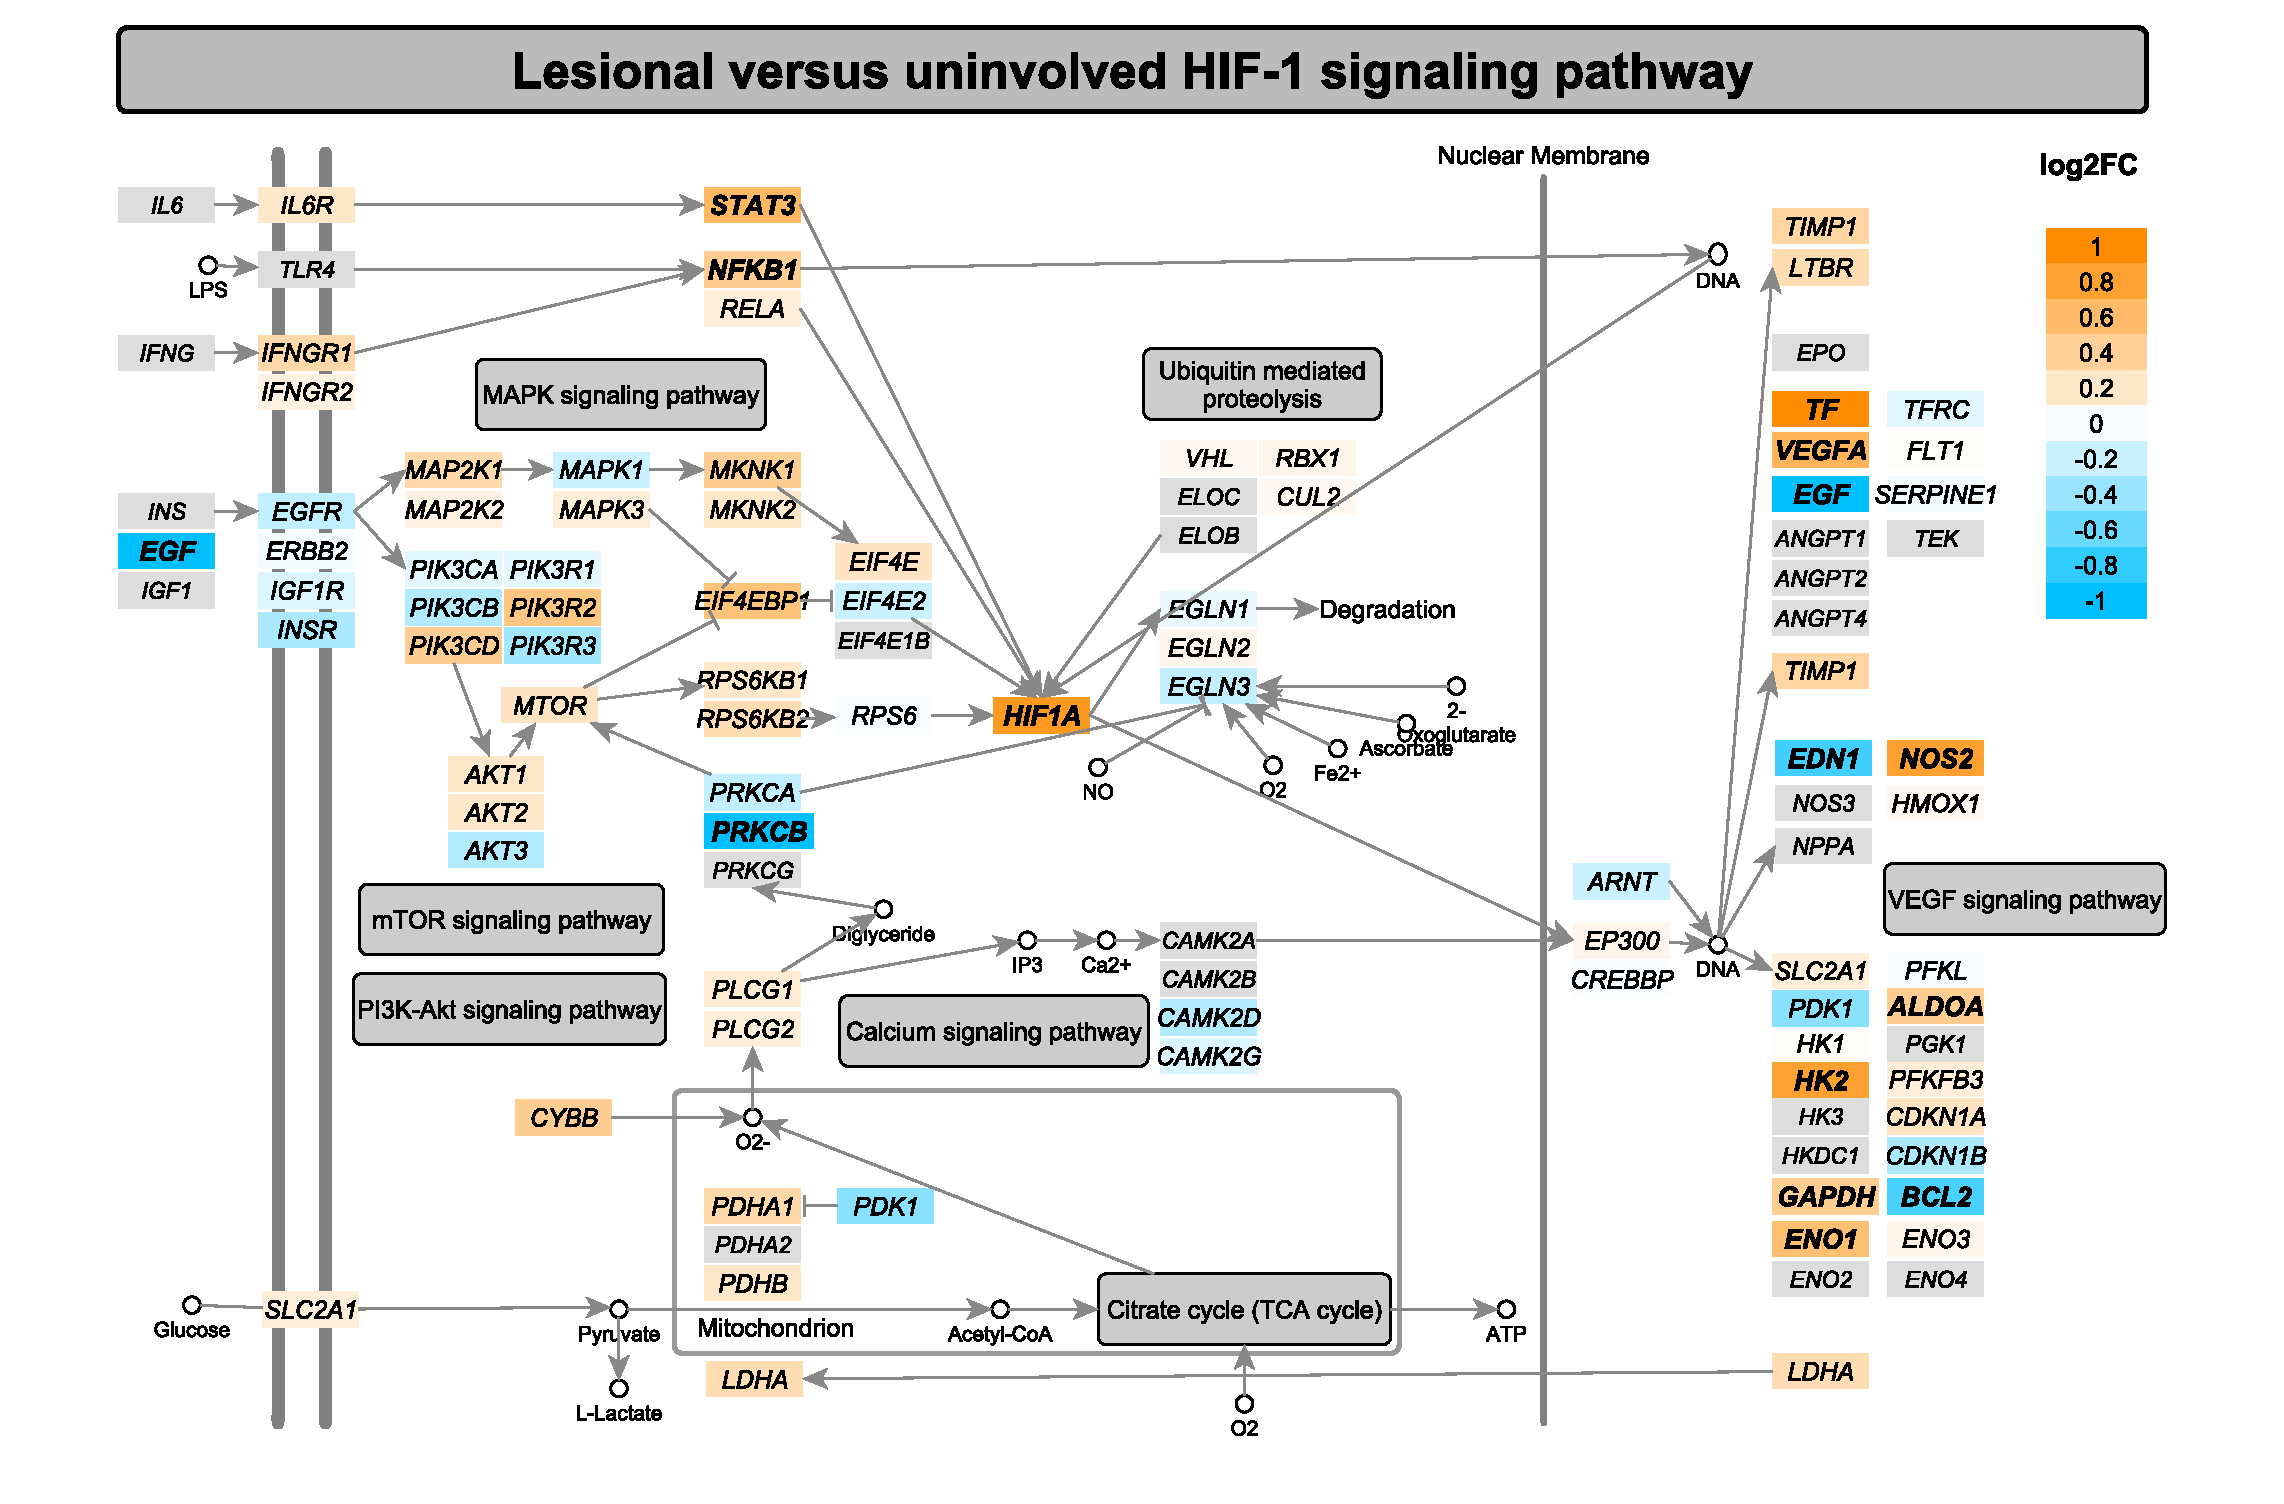
\includegraphics[width=0.9\textwidth]{./Results2/pdfs/PS_lesional_uninvolved_all_HIF_1_pathway}
\caption[Mapping of the DEGs between lesional and uninvolved epidermis from psoriasis patients onto the HIF-I signalling pathway.]{\textbf{Mapping of the DEGs between lesional and uninvolved epidermis from psoriasis patients onto the HIF-I signalling pathway.} This pathway was sourced from KEGG, manually curated in a way that all member genes are maximised visually and then automatically color-coded by the log$_2$FC expression between the lesional and uninvolved epidermis. Significant DEGs (FDR$<$0.05) are highlighted in bold. This pathway was identified by pathway enrichment analysis using only DEGs (FDR$<$0.05).}
\label{figure:PS_lesional_vs_uninvolved_HIF_pathway}
\end{figure}

Immune relevant pathways including IFN, IL-17 and NOD-like receptor signalling were also identified in this analysis. The NOD-like receptor pathway responsible for detecting various pathogens and generating innate immune responses through NF-$\kappa$B and MAPK activation, appeared enriched with 23 significantly DEGs (Figure \ref{figure:PS_lesional_vs_uninvolved_HIF_pathway} in orange and bold). %This pathway has also been identified as one of the most significantly enriched for DEGs in the epidermal study of Tervaniemi and colleagues. 
Some of the most up-regulated genes contributing to the enrichment included \textit{NOD2}, \textit{CARD6} or \textit{IFI16}, amongst others, and they were also up-regulated in Tervaniemi's data, where 42 DEGs mapped to this pathway. Amongst the down-regulated genes contributing to this pathway were \textit{TNFAIP3} and \textit{BCL-2} (Figure \ref{figure:PS_lesional_vs_uninvolved_HIF_pathway} in blue and bold). Performing pathway enrichment analysis using the DEGs from Tsoi and colleagues failed to show significant enrichment for NOD-like receptors signalling (19 DEGs in the NOD-like pathway). Nevertheless, NOD-like receptors signalling remained significantly enriched (13 DEGs mapping to this pathway) when the analysis was conducted using only the DEGs from the in-house data not overlapping the Tsoi and colleagues results. 
%These findings highlight the failure of whole skin biopsies transcriptomics to identify additional NOD-I signalling genes differentially regulated between lesional and uninvolved skin and the value of studying epidermal biopsies to unveil exacerbated dysregulation of functional pathways in KCs.


\begin{landscape}
\begin{figure}[H]
\centering
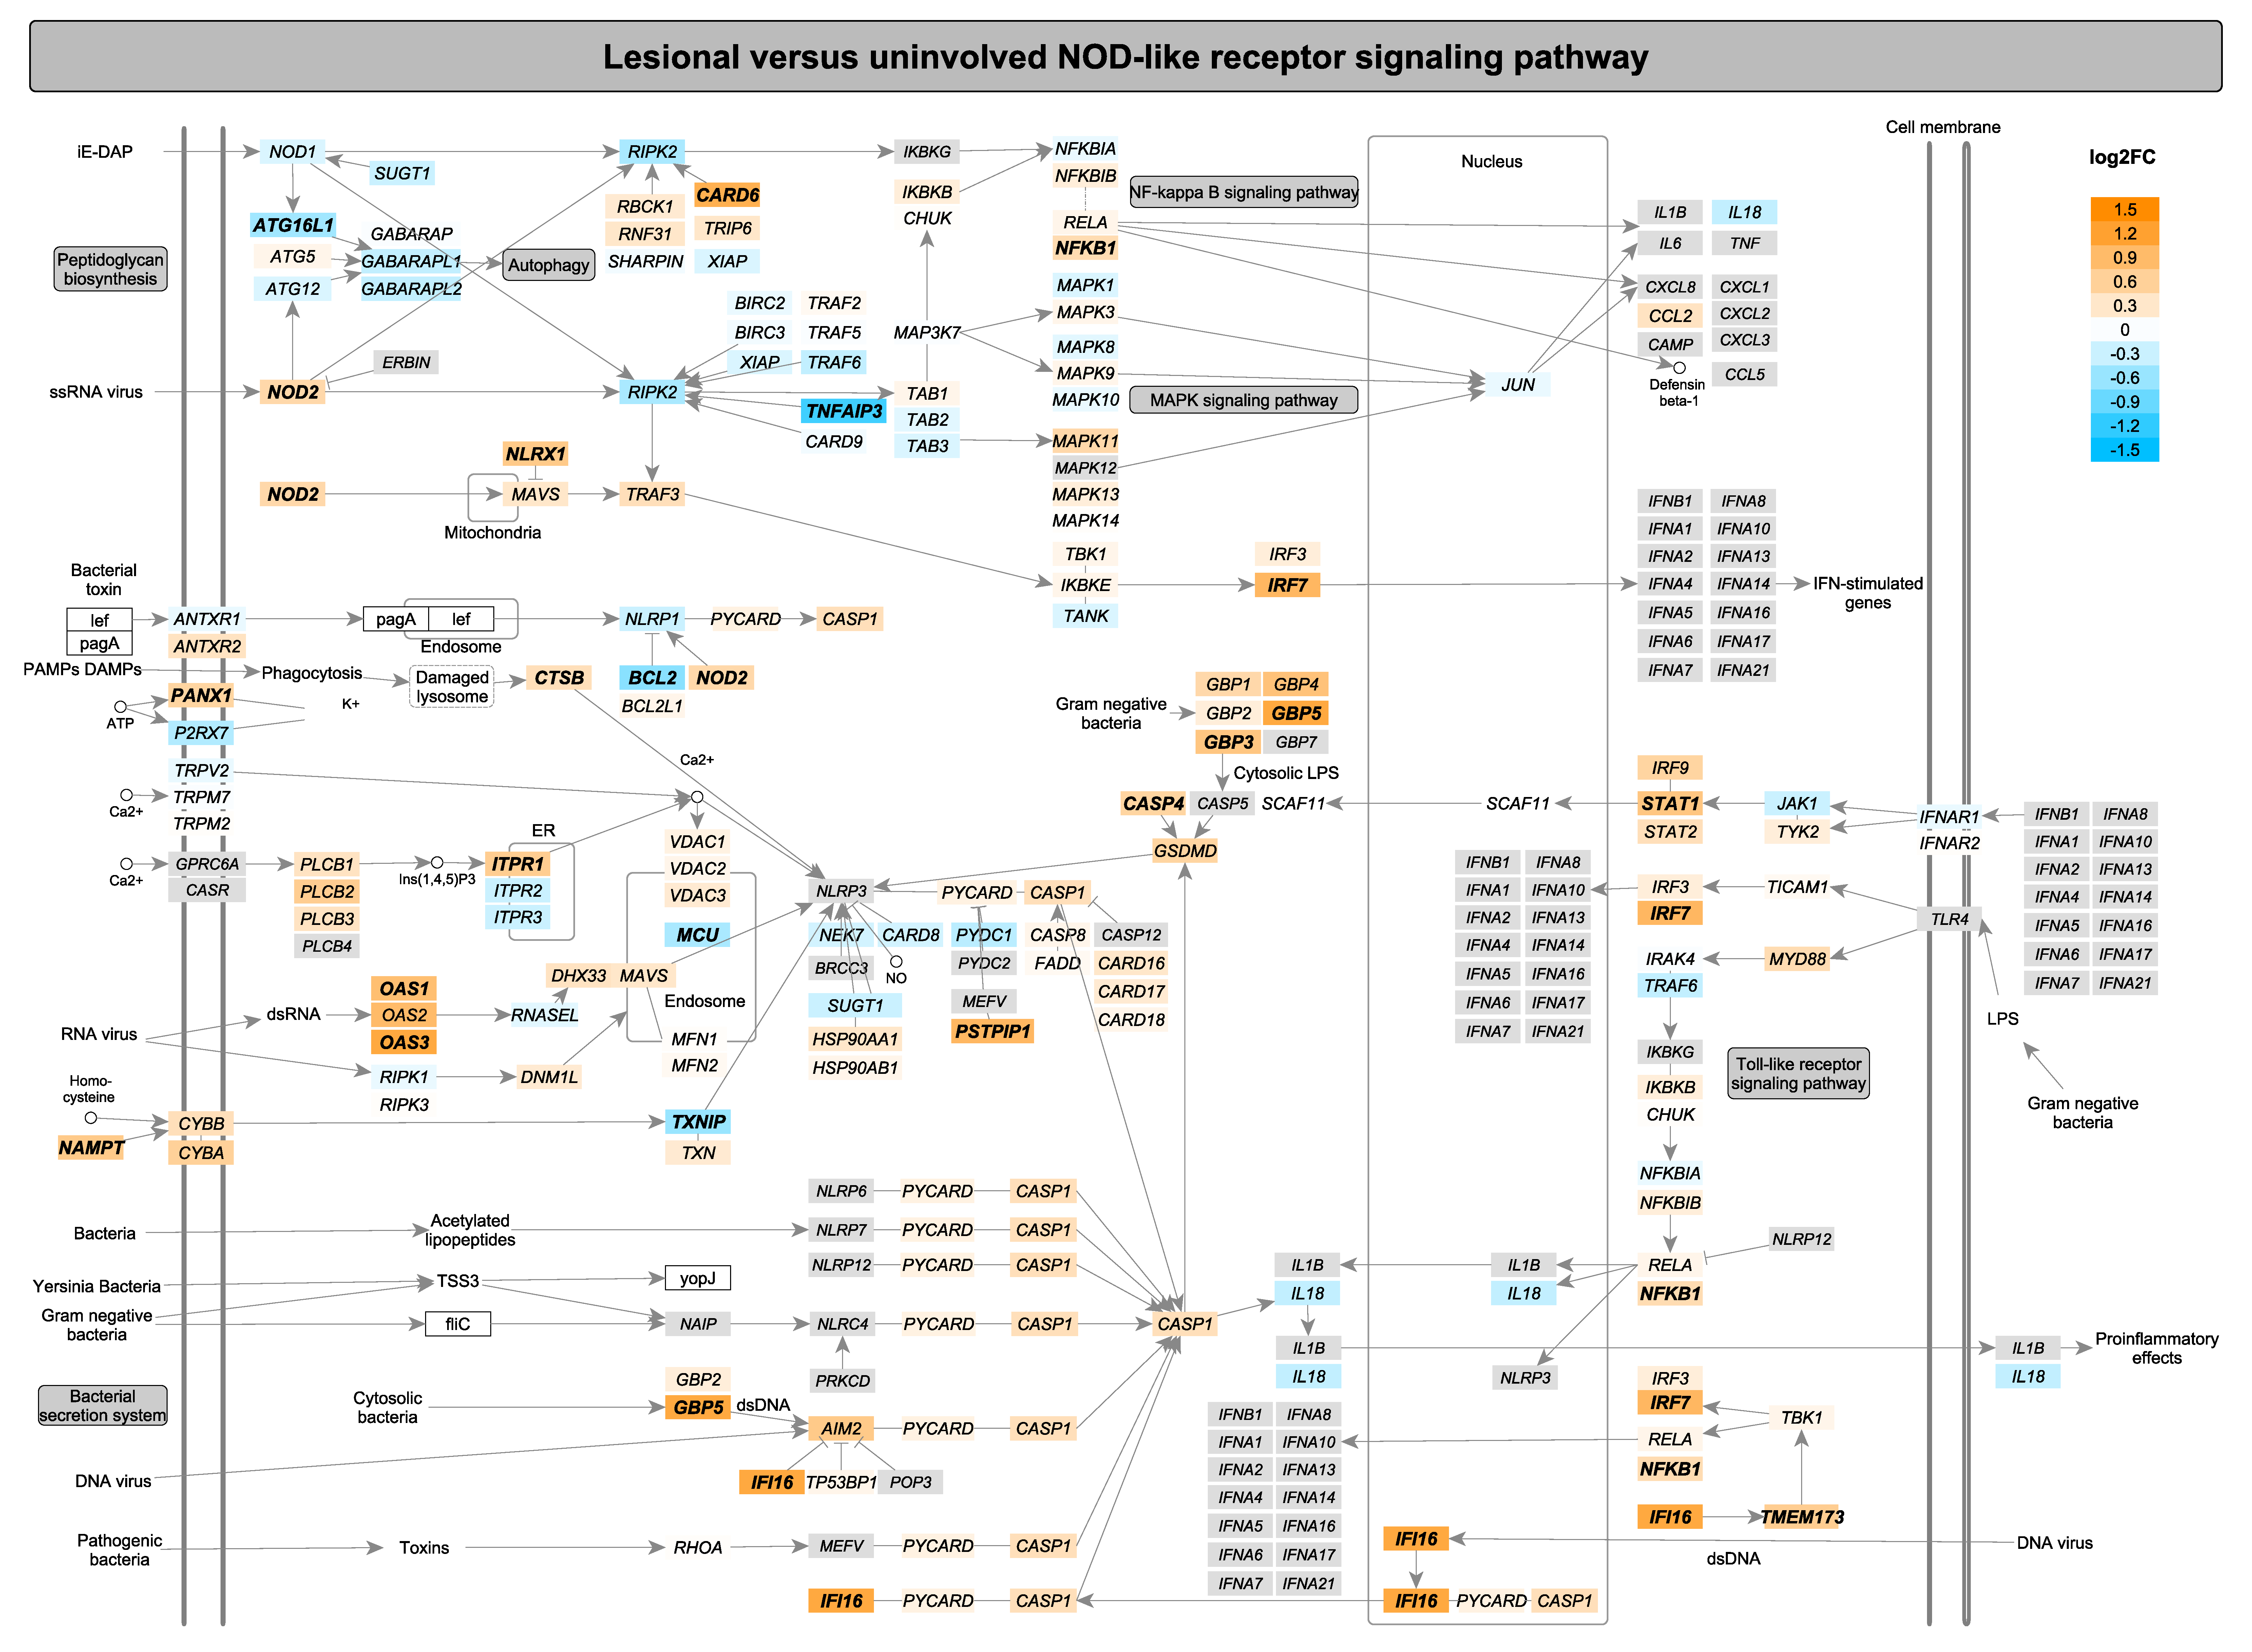
\includegraphics[width=\textwidth]{./Results2/pdfs/PS_lesional_uninvolved_all_NOD_like_pathway}
\caption[Mapping of the DEGs between lesional and uninvolved epidermis from psoriasis patients onto the NOD-like signalling pathway.]{\textbf{Mapping of the DEGs between lesional and uninvolved epidermis from psoriasis patients onto the NOD-like signalling pathway.} This pathway was sourced from KEGG, manually curated in a way that all member genes are maximised visually and then automatically color-coded by the log$_2$FC expression between the lesional and uninvolved epidermis. Significant DEGs (FDR$<$0.05) are highlighted in bold. This pathway was identified by pathway enrichment analysis using only DEGs (FDR$<$0.05).}
\label{figure:PS_lesional_vs_uninvolved_HIF_pathway}
\end{figure}
\end{landscape}


In addition to the NOD-I signalling, IL-17 signalling was another enriched pathway well known to be relevant in the development of psoriasis. Enrichment of the IL-17 signalling pathway in our data is driven by up-regulation of the S100 protein family (\textit{S100A7}, \textit{S100A8} and \textit{S100A9}) and chemokines such as \textit{CCL20}, which binds the CCR6 receptor and is involved in DCs and T cell chemotaxis. \textit{IL-17RE} which together with IL-17RA forms the receptor for IL-17C was down-regulated in lesional skin, similarly to Tsoi and Tervaniemi's data, which found up-regulation for a number of these genes. Dysregulation for other IL-17 ligands and receptors or IL-23A was neither detected, in contrast to the observations from Tsoi and Tervaniemi. Moreover, enrichment of DEGs between lesional and uninvolved skin for the peroxisome proliferator-activated receptor (PPAR) signalling highlighted the link between metabolic dysregulation (particularly lipids) and innate immunity. This pathway included up-regulation of the PPAR receptor $\delta$ (\textit{PPARD}), stearoyl-CoA desaturases such as \textit{SCD} and \textit{SCD5} involved in fatty acid synthesis and \textit{CD36} which mediates fatty acid transport, also dysregulated in the Tsoi and/or Tervaniemi studies.

%contributing to the psoriasis pathophysiology and increased risk of co-morbidities, such as metabolic syndrome and CVD. 

%PPARs are ligand-dependent TF that have been shown to induce the inhibition of pro-inflammatory genes including IL-1 and TNF-$\alpha$ \parencite{Ji2001}. In skin, PPARs have been demonstrated to contribute to homeostasis by inducing differentiation and preventing proliferation \parencite{Rivier1998}. Moreover, inhibition of genes regulated by PPAR-$\gamma$ has been described in studies comparing lesional versus healthy skin biopsies \parencite{Li2014}.
%CCL20 https://www.ncbi.nlm.nih.gov/pubmed/19295614
%CCR6-CCL20 Dendritic Cells Rapidly Recruited into Epithelial Tissues via CCR6/CCL20 Are Responsible for CD8+ T Cell Crosspriming In Vivo

%Also sharing ECM, cell junctions and pathwsys in cancer, in our case microRNAs.


\subsection{Comparison of the systemic and tissue-specific gene expression signatures in psoriasis}

In order to describe commonalities and differences in psoriasis gene expression at the affected tissue (skin) and the systemic level (circulating immune cells), overlap between the lists of DEGs was performed. Only modest overlap was found between dysregulated genes in lesional skin compared to uninvolved and the DEGs identified in circulating immune cells, with CD14$^+$ monocytes and tCD8$^+$ cells showing the greatest overlap. A similar or larger proportion of the total overlapping DEGs presented opposite direction of change in circulating immune cells and in skin from psoriasis patients. An examples was \textit{TNFAIP3} gene, which was up-regulated in psoriasis tCD4$^+$ and tCD8$^+$ cells compared to controls and down-regulated in lesional epidermis when compared to uninvolved.  
%In Tsoi \textit{et al.}, 2015 this gene did not change expression between lesional and uninvolved nor between lesional and healthy skin and Li \textit{et al.}, reported its up-regulation in lesional skin. 

Another two relevant transcript showing opposite dysregulation were the early growth response 1 and 3 (\textit{EGR1} and \textit{EGR3}) genes, two genes involved in maintenance of the homeostasis of the adaptive immune response \parencite{Li2012}. Both genes were up-regulated in CD14$^+$ monocytes in psoriasis compared to controls and \textit{EGR2} was also up-regulated in tCD4$^+$ cells. Conversely, great up-regulation of \textit{EGR2} and \textit{EGR3} (log$_{2}$FC -0.74 and -0.53) was observed in 
lesional skin when compared to uninvolved. Interestingly, no overlap was observed for genes of the \textit{S100} family, only found to be up-regulated in lesional skin. Lastly, the previously described \textit{MIR146A} also appeared dysregulated in opposite direction in tCD8$^+$ cells and in the skin analysis, presenting down- and up-regulation, respectively.

 
%EGR2 and 3 https://www.ncbi.nlm.nih.gov/pmc/articles/PMC3477314/

\begin{table}[htbp]
%\setlength{\tabcolsep}{20pt} only to stretch the columns if you want
%\renewcommand{\arraystretch}{1.5}
\centering
\begin{tabular}{@{} c c c c}
\toprule
\textbf{DEGs overlapping}   & \textbf{Total overlap}   & \textbf{Same direction}  & \textbf{Opposite direction}\\
\textbf{with skin}          &                          &                          &                            \\
\midrule 
\midrule
CD14$^+$ monocytes          & 37                       & 19                       &  18                         \\ 
tCD4$^+$                     & 10                       & 6                        &  4                           \\
tCD8$^+$                     & 37                       & 24                       &  13                           \\
CD19$^+$                    & 16                       & 5                        &  11                          \\
\bottomrule 
\end{tabular}
\medskip %gap
\caption[Overlap between the DEGs in the four circulating immune cell types (psoriasis patients versus controls) and the DEGs in psoriasis patients skin biopsies (lesional versus uninvolved).]{\textbf{Overlap between the DEGs in the four circulating immune cell types (psoriasis patients versus controls) and the DEGs in psoriasis patients skin biopsies (lesional versus uninvolved).} DEGs based on FDR$<$0.05 for each of the comparisons} 
\label{tab:RNAseq_overlap_circulating_versus_skin}
\end{table}
\bigskip %bigger spac

%Talk about NOD genes overlapping the circulation DEGs
%Mention about IFN pathway

The limited overlap between circulating and skin DEGs was also reflected in the different enriched pathways identified for each analysis. The pathways enriched for CD14$^+$ and tCD8$^+$ DEGs were mostly immune-related pathways, including TCR , IL-12 , TNF and NF-$\kappa$B signalling. Moreover,some of the pro-inflammatory genes contributing to those pathways appeared down-regulated in psoriasis when compared to controls, as previously commented.% some of the genes in these circulating immune cells suggested certain immuno-supression features that could be characteristic of these cells before or/and after having been exposed to the skin inflammatory \textit{milieu}. 
In skin, the DEGs in lesional epidermis when compared to uninvolved were not only enriched in immune-related pathways but also for pathways involved in metabolism, oxidative stress and cell cycle. In contrast to the systemic observation, the dysregulation of genes contributing to the enrichment of immune-related pathways appeared to present a more clear pro-inflammatory signature, which would be consistent with the skin being a site of more active inflammation compared to circulating immune cells in psoriasis.


\subsection{Integration of chromatin accessibility and expression data in circulating immune cells}
The characterisation of the chromatin accessibility landscape and the transcriptome in circulating immune cells from psoriasis patients has revealed a greater effect of disease in gene expression than in chromatin accessibility. In order to assess to some extent the relationship between the two, overlap between DEGs and the genes proximal to DARs ($\leq$5Kb) was performed. Overlap was only found in CD8$^+$ cells, where 6 out of the 53 DARs were annotated by proximity to an RNA-seq DEG in the same cell type (\textit{ARL4A}, \textit{ASCL2}, \textit{ENTPD1}, \textit{TIAM1}, \textit{TRAT1} and \textit{ZNF276}). 

An example was T Cell lymphoma invasion and metastasis 1 (\textit{TIAM1}), which activates IL-17 expression and T cell transendothelial migration during inflammation \parencite{Kurdi2016, Gerard2009}. This gene showed an increased expression (log$_2$FC 0.44) in psoriasis patients tCD8$^+$ cells (Figure \ref{figure:ATAC_RNAseq_CD8_TIAM1_combined} left). Likewise, psoriasis CD8$^+$ cells presented greater chromatin accessibility compared to healthy controls (log$_2$FC 0.41) in a region located at an intron of the \textit{TIAM1} gene and annotated as an active enhancer according to the Roadmap chromatin segmentation data in this cell type (Figure \ref{figure:ATAC_RNAseq_CD8_TIAM1_combined} right). Common SNPs within this peak did not appear to be an eQTL regulating expression of any gene in tCD8$^+$ cells \parencite{Kasela2017} and chromatin conformation data did not reveal interaction of this particular region with the \textit{TIAM1} promoter \parencite{Javiere2016}, at least in unstimulated conditions, complicating the establishment of a mechanistic connection between chromatin accessibility and gene expression.

Another two relevant genes in the immune response for which ATAC and RNA-seq presented overlap were the ectonucleoside triphosphate diphosphohydrolase 1 (\textit{ENTPD1}), which hydrolyses the pro-inflammatory mediator ATP attenuating the inflammation and acting as a modulator of the immune response, and the TCR-associated transmembrane adaptor 1 (\textit{TRAT1}) gene, a positive regulator of TCR signalling \parencite{Antonioli2013, Valk2006}. Both genes presented up-regulated expression and increased chromatin accessibility in psoriasis patients tCD8$^+$ cells compared to healthy controls.

% mention about TIAM1 being a good target in Pi
%short check for the ENTPD1 and TRAT1 DARs to be likely to affect 

\begin{figure}[htbp]
\centering
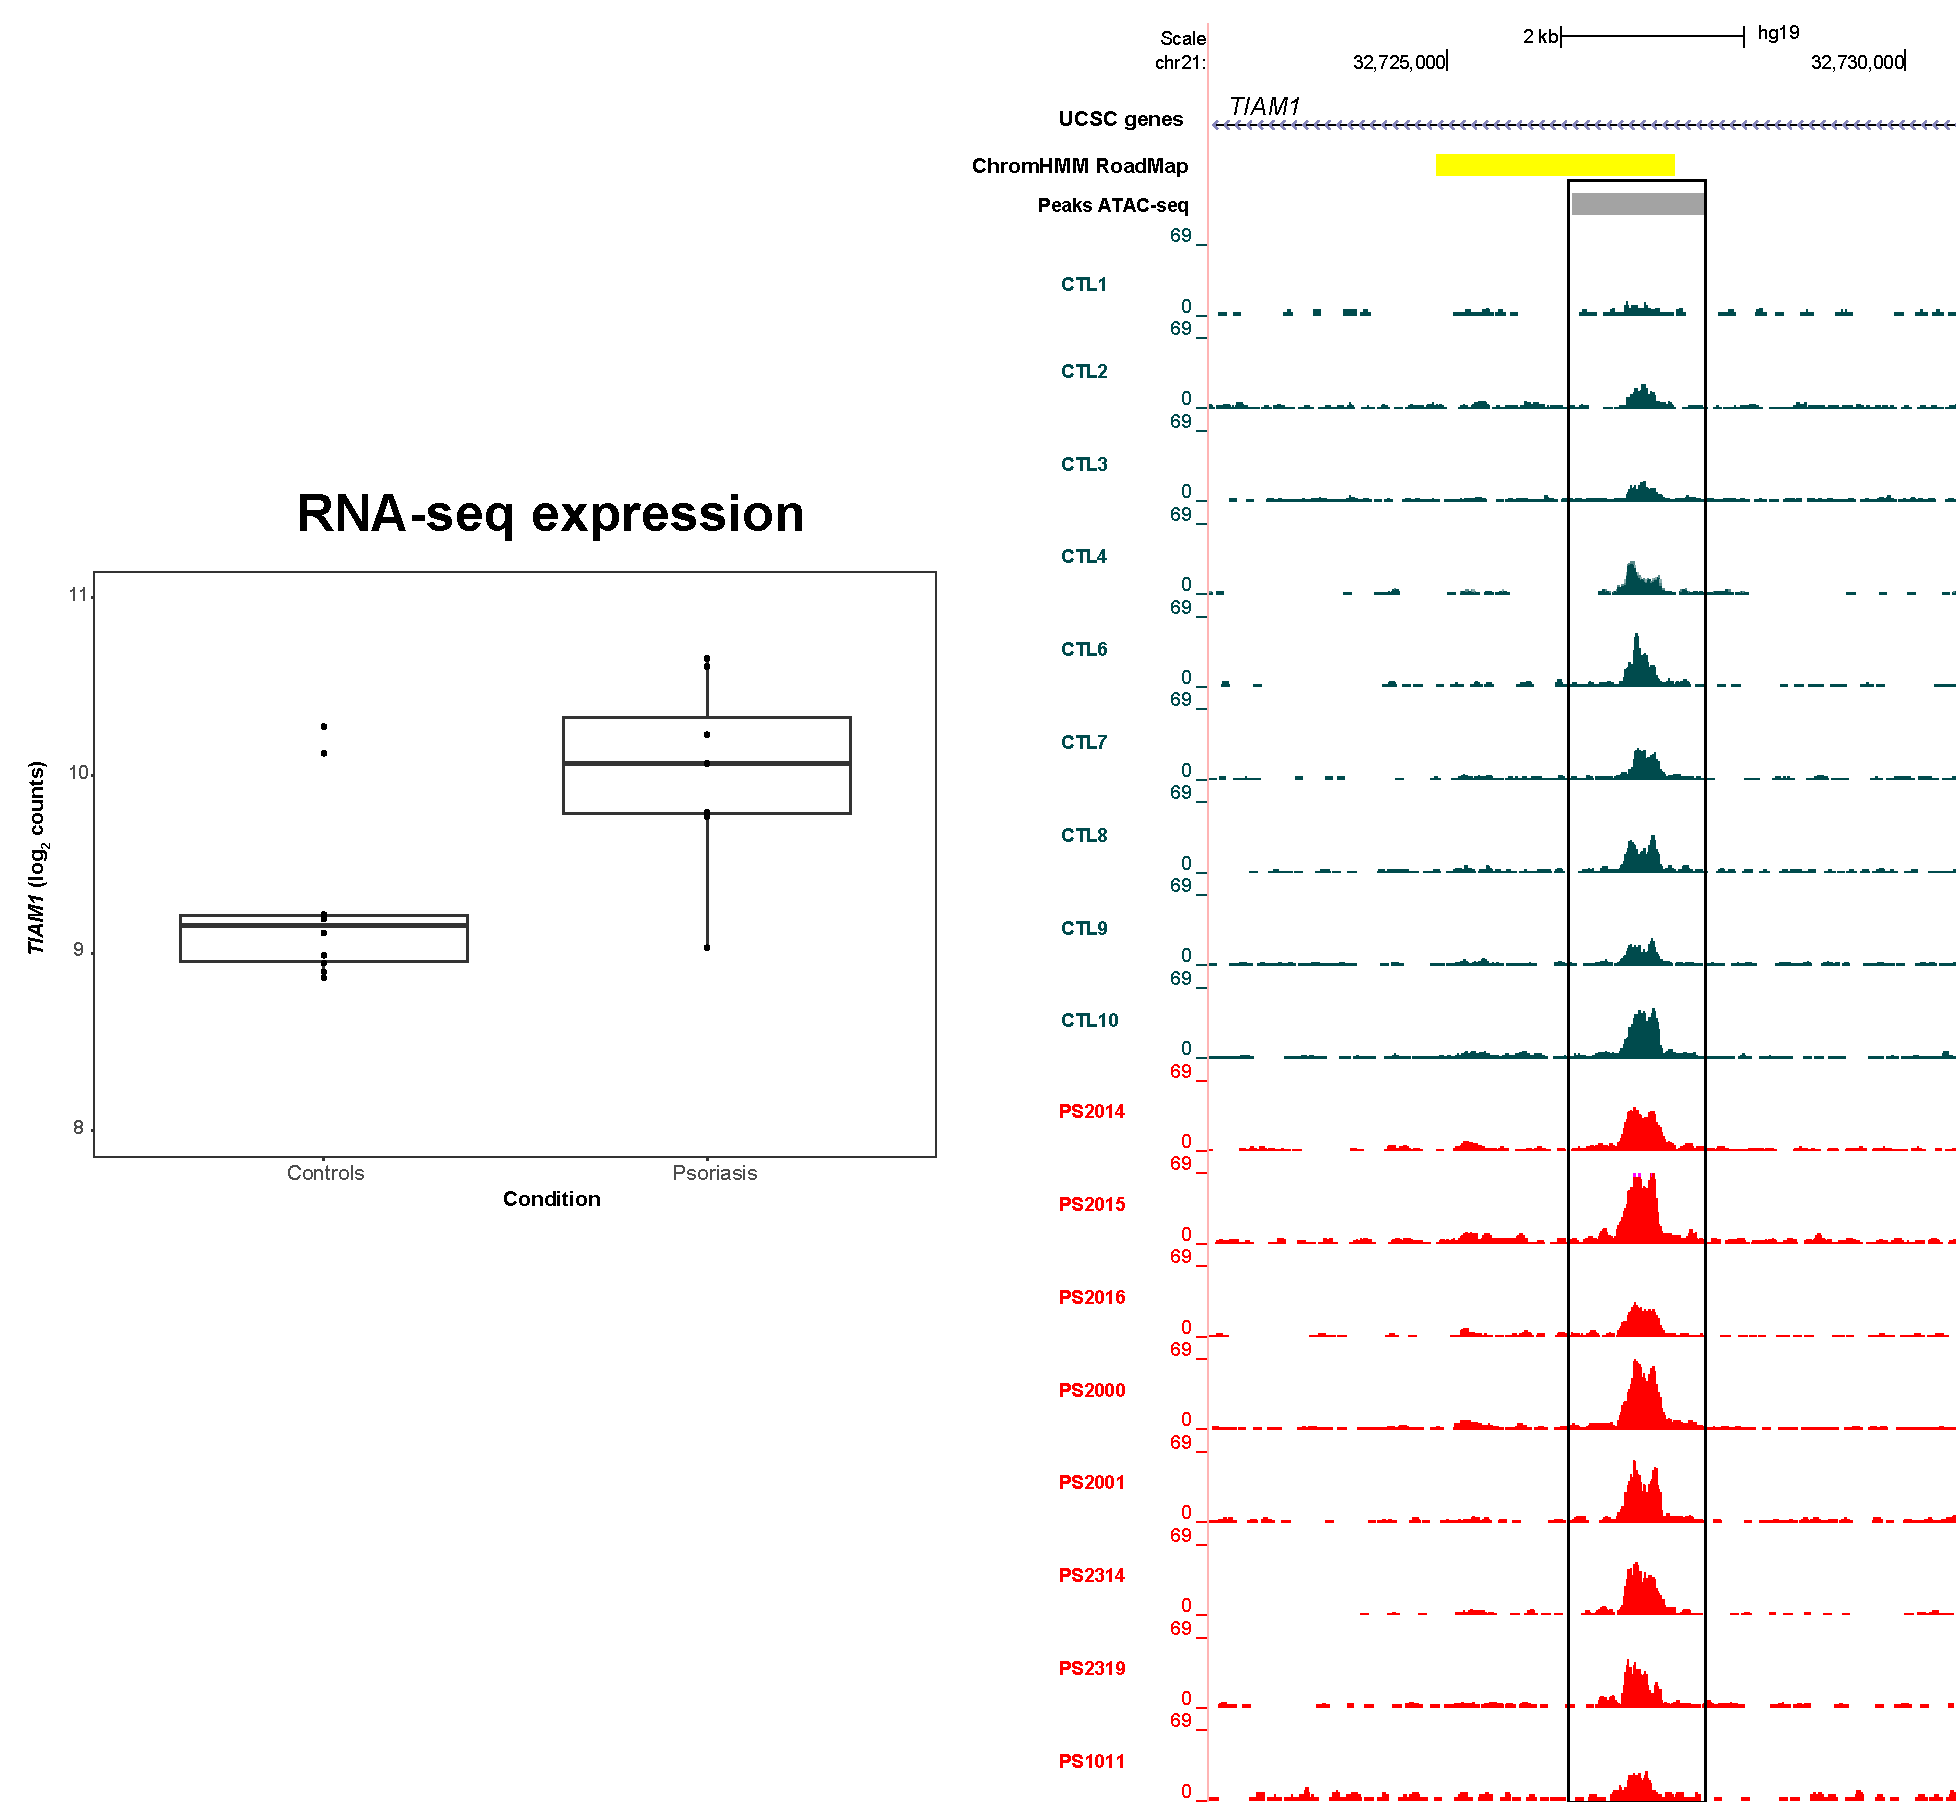
\includegraphics[width=0.65\textwidth]{./Results2/pdfs/ATAC_CD8_peak_TIAM1_RNA_combined}
\caption[Differential gene expression and chromatin accessibility landscape for \textit{TIAM1} gene in tCD8$^+$ cells.]{\textbf{Differential gene expression and chromatin accessibility landscape for \textit{TIAM1} gene in tCD8$^+$ cells.} Boxplot on the left represents RNA-seq log$_{2}$ normalised counts for the \textit{TIAM1} gene in psoriasis and healthy controls tCD8$^+$ cells. The right panel is the UCSC Genome Browser view illustrating the normalised ATAC read density (y-axis) at an intron of the \textit{TIAM1} gene (x-axis) in tCD8$^+$ cells. This region was identified as more accessible in psoriasis patients compared to healthy controls. Tracks are colour-coded by condition and assay: control(CTL)=dark turquoise and psoriasis (PS)=red. The Epigenome Roadmap chromatin segmentation map for tCD8$^+$ cells is included.}
\label{figure:ATAC_RNAseq_CD8_TIAM1_combined}
\end{figure}



\subsection{Fine-mapping of psoriasis GWAS loci and functional interpretation}

\subsubsection{Fine-mapping using summary statistics data}
In absence of permission to access genotyping data, fine-mapping of psoriasis Immunochip GWAS loci was conducted using summary statistics of the GAPC cohort (2,997 cases and 9,183 controls), one of the two included in the Immunochip psoriasis GWAS study from Tsoi \textit{et al.}, 2012. Summary statistics of the second cohort genotyped using the Immunochip in Tsoi and colleagues' publication (PAGE cohort) were not publicly available through ImmunoBase at the time of this analysis. As explained in Chapter \ref{ch:Mat}, fine-mapping from summary statistics with DIST uses the statistics z-score of each of the genotyped SNPs to impute z-scores for the missing SNPs based on the r$^2$ relationship from the 1000 Genome Project Version 3 \parencite{Lee2013}. Following z-score imputation, association analysis is performed and ABF, PP and credible set of SNPs are built for each of the signals. 

Fine-mapping was performed for 26 of the Immunochip GWAS loci reported by Tsoi \textit{et al.}, 2012, excluding the MHC and those loci which were in high LD with missense mutations showing experimentally proved or with highly confident predicted damaging effects. Out of the 26 regions, 9 loci did not reach log$_{10}$ABF$>$3 (cut-off used as in Bunt \textit{et al.},2015) with 90\% credible sets ranging from 19 to 853 SNPs (Table \ref{tab:Psoriasis_loci_no_fine_mapping}). Of the 17 loci presenting log$_{10}$ABF$>$3, the fine-mapping lead SNP was in low LD with the Tsoi \textit{et al.},2012 GWAS lead SNP, which was not included in the credible set (Table \ref{tab:Psoriasis_fine_mapping_summary} with $^\ast$). This is likely due to the effect of reduced sample size, (only GAPC cohort) compared to Tsoi \textit{et al.},2012, on the ability to identify association signals \parencite{Bunt2015}. 




\begin{landscape}
\begin{center}
%\begin{longtable}[ht]{p{.25\textheight} p{.40\textheight} p{.25\textheight} p{.60\textheight}}
\begin{longtable}[ht]{c c c c c c c c c}
\caption[Summary table of the psoriasis Immunochip GWAS loci presenting log${_10}ABF>3$ for the fine-mapping lead SNP.]{\textbf{Summary table of the psoriasis Immunochip GWAS loci presenting log${_10}ABF>3$ for the fine-mapping lead SNP.} For 16 of the Immunochip psoriasis GWAS loci presented log${_10}ABF>3$ the table reports the closer gene(s), FM lead SNP, MAF, OR for the GAPC cohort, log${_10}ABF$ for the FM lead SNP, PP, number of SNPs included in the 90\% credible set and the Tsoi \textit{et al.},2012 GWAS lead SNP. In 10 of those loci ($^{\ast}$) the fine-mapping lead SNP was in low LD (r${^2}<0.5$) with the psoriasis GWAS SNP and did not contain it in the credible set. FM=fine-mapping; MAF= minor allele frequency; OR=odds ratio; ABF=approximate Bayes factor; PP=posterior probability.}
\label{tab:Psoriasis_fine_mapping_summary} \\
\toprule
\textbf{chr} & \textbf{Closer} & \textbf{FM} & \textbf{MAF} & \textbf{OR} & \textbf{log${_10}ABF$} & \textbf{PP} & \textbf{90\% credible} &\textbf{Tsoi} \\
             & \textbf{gene} & \textbf{lead SNP} &          & \textbf{GAPC} & \textbf{FM lead SNP} &             & \textbf{set}           &\textbf{lead SNP} \\
\midrule
\midrule
1	& \textit{IL28RA}&	     rs61774731$^{\ast}$   &		0.10 &		1.21 &		11.5 &		0.99 &		1	 &	rs7552167 \\
2	& \textit{FLJ16341/REL}& rs6714339$^{\ast}$    &		0.14 &		1.17 &		9.0  &		0.99 &		1	 &	rs62149416 \\
2	& \textit{IFIH1}&		     rs2111485$^{\ast}$    &		0.59 &		1.27 &		6.7  &		0.50 &		2	 &	rs17716942 \\
5	& \textit{TNIP1}&		     rs17728338            &		0.06 &		1.59 &		10.6 &		0.40 &		6	 &	rs2233278 \\
5	& \textit{IL12B/ADRA1B}& rs12188300            &		0.05 &		1.58 &		11.2 &		0.18 &		9	 &	rs12188300 \\
6	& \textit{TNFAIP3}&		   rs1416173$^{\ast}$    &		0.85 &		1.23 &		7.7  &		0.15 &		10 &		rs582757 \\
14	& \textit{NFKBIA}&		 rs74243591            &		0.21 &		1.16 &		5.0  &		0.30 &		12 &		rs8016947 \\
17	& \textit{NOS2}&		   rs117094752$^{\ast}$  &		0.02 &	  1.22 &		7.3  &		0.94 &		1  &		rs28998802 \\
1	& \textit{SLC45A1/TNFRSF9}&		rs425371         &		0.25 &    1.13 &		5.6  &		0.14 &		22 &		rs11121129 \\
1	& \textit{RUNX3}&		     rs61774731 $^{\ast}$  &		0.10 &		1.13 &		11.5 &		0.99 &		1  &		rs7536201 \\
2	& \textit{B3GNT2/TMEM17}&		rs9309343$^{\ast}$ &		0.33 &		1.12 &		4.3  &		0.66 &		34 &		rs10865331 \\
7	& \textit{ELMO1}&		     rs77840275$^{\ast}$   &		0.10 &		1.11 &		7.5  &		0.99 &		1  &		rs2700987 \\
11	& \textit{ZC3H12C}&		 rs11213274            &		0.40 &		1.14 &		4.0  &		0.05 &		69 &		rs4561177 \\
16	& \textit{PRM3/SOCS1}& rs111251548$^{\ast}$  &		0.02 &		1.13 &		9.4  &		0.97 &		1  &		rs367569 \\
17	& \textit{PTRF/STAT3}& rs963986              &		0.17 &		1.15 &		4.1  &		0.18 &		8  &		rs963986 \\
19	& \textit{ILF3/CARM1}& rs34536443$^{\ast}$   &		0.03 &		1.17 &		9.7  &		0.93 &		1  &		rs892085 \\
\bottomrule
%\medskip
\end{longtable}
\end{center}
\end{landscape}


The 6 loci including the Tsoi \textit{et al.},2012 lead GWAS SNP presented a number of SNPs in the 90\% credible set of SNPs ranging from 6 to 69 (Table \ref{tab:Psoriasis_fine_mapping_summary}). Of those 6 loci, \textit{TNIP1}, \textit{IL12B/ADRA1B} and \textit{PTRF/STAT3} had 90\% credible sets which included less than 10 SNPs. \textit{TNIP1} and \textit{IL12B/ADRA1B} had been previously fine-mapped by Das and colleagues using dense genotyping with a customised array followed by association analysis \parencite{Das2014}. Interestingly, 2 (rs75851973 and rs2233278) and 3 SNPs (rs918519, rs918518 and rs733589) from the \textit{TNIP1} and \textit{IL12B/ADRA1B} 90\% credible sets, respectively, were amongst the set of significant variants and perfect near proxies (r$^2>0.9$) reported  by Das \textit{et al.} for those two same loci.



\subsubsection{Integration with functional data}
A total of 126 unique SNPs formed the union of 90\% credible sets from the 6 loci with fine-mapped lead SNPs presenting a log$_{10}ABF>$3 and including the Tsoi \textit{et al.},2012 GWAS lead SNP. None of the SNPs overlapped any of the DARs or differentially H3K27ac regions identified in CD14$^+$ monocytes, tCD4$^+$, tCD8$^+$ and CD19$^+$ cells. Conversely, overlap with the consensus master list ATAC peaks from each of the cell types revealed a total of 16 SNPs from 5 loci located at accessible chromatin in at least one cell type (\textit{NFKBIA}(1 SNP), \textit{PTRF/STAT3}(1 SNP), \textit{SLC45A1/TNFRSF9}(4 SNPs), \textit{TNIP1}(4 SNPs) and \textit{ZC3H12C}(6 SNPs)). However, no overlap was found for the 9 SNPs of the \textit{IL12B/ADRA1B} 90\% credible set. CD14$^+$ monocytes appeared as the cell type showing the largest proportion of accessible chromatin regions containing SNPs from the credible (2.3\%), followed by CD19$^+$, tCD4$^+$ and tCD8$^+$ cells (1.7, 1.6 and 1.05\%, respectively) (Table \ref{tab:Psoriasis_fine_mapping_ATAC_overlap}). Altogether, integration of the SNPs from the credible set with ATAC accessible regions in four cell types allowed to further refine the number of genetic variants with a putative functional role in psoriasis for 5 of the 6 analysed loci. Moreover, in the \textit{PTRF/STAT3} and \textit{SLC45A1/TNFRSF9} loci all the SNPs from the credible set overlapping accessible chromatin appeared to be cell type specific (Table \ref{tab:Psoriasis_fine_mapping_summary} and \ref{tab:Psoriasis_fine_mapping_ATAC_overlap}). Of the 8 SNPs in the \textit{PTRF/STAT3} credible set, only 1 overlapped accessible chromatin in CD14$^+$ monocytes. Similarly, the \textit{SLC45A1/TNFRSF9} locus presented only 4 out of the 22 SNPs from the 90\% credible set within ATAC peaks, of which all were CD14$^+$ monocytes-specific.   

\begin{table}[htbp]
%\setlength{\tabcolsep}{20pt} only to stretch the columns if you want
%\renewcommand{\arraystretch}{1.5}
\centering
\begin{tabular}{@{} c c c}
\toprule
\textbf{ATAC cell type} & \textbf{90\% credible set}   &  \textbf{Cell type specific}  \\
\textbf{master list}    & \textbf{overlapping SNPs}    &   \textbf{overlap}   \\
									      &	\textbf{(number)}				     &                            \\
\midrule
\midrule
 CD14$^+$ monocytes    & 13                            &  \textit{PTRF/STAT3}(1),\\ 
                       &                               &  \textit{SLC45A1/TNFRSF9}(4)\\
 tCD4$^+$              & 5                             &  None \\
 tCD8$^+$              & 3                             &  \textit{TNIP1} (2)        \\
 CD19$^+$              & 5                            &  None     \\
\bottomrule
\end{tabular}
\medskip %gap
\caption[SNPs from the 90\% credible set of the successfully fine-mapped psoriasis loci overlapping ATAC accessible chromatin in four cell types.]{\textbf{SNPs from the 90\% credible set of the successfully fine-mapped psoriasis loci overlapping ATAC accessible chromatin in four cell types.} The number of SNPs in the 90\% credible set union (total 126 SNPs) from the 6 successfully fine-mapped loci overlapping ATAC accessible chromatin in each cell type master list are reported. Additionally, the number of SNPs only found to overlap open chromatin in one cell type are indicated together with the locus in which the SNP was fine-mapped.}
\label{tab:Psoriasis_fine_mapping_ATAC_overlap}
\end{table}



\subsubsection{The functional landscape at \textit{SLC45A1/TNFRSF9} locus}

As previously mentioned, integration of the \textit{SLC45A1/TNFRSF9} 90\% credible set of SNPs with ATAC data further refined the number of candidate functional SNPs from 22 to 4. \textit{SLC45A1/TNFRSF9} was one of the new intergenic GWAS associations reported by Tsoi \textit{et al.}, 2012 and is shared with UC and celiac disease (\url{https://www.immunobase.org/}). Amongst the 4 SNPs overlapping CD14$^+$ monocyte ATAC-specific peaks was the fine-mapping lead SNP rs425371, which is located at an intergenic region, approximately 269.3Kb downstream \textit{TNFRSF9} gene. The other three SNPs overlapping CD14$^+$ monocytes accessible chromatin included rs11121131, rs12745477 and rs417065. 




\subsection{Maximising genetic commonalities across chronic inflammatory diseases: locus 2p15}
The chr2p15 psoriasis risk locus (lead SNP rs10865331, OR=1.12) represents one of the GWAS associations located in an intergenic region was identified by the Immunochip study from Tsoi \textit{et al.},2012. This locus is shared with the chronic inflammatory diseases AS and CD. Interestingly, Reveille's AS GWAS study reported the same lead SNP as the psoriasis Immunochip \parencite{Reveille2010}. The later AS Immnochip study identified rs6759298 (OR=1.29) as the tag SNP for this region, which is in high LD (r$^2$=0.84) with rs10865331 \parencite{Cortes2012}. A recent GWAS meta-analysis combining data for five chronic inflammatory diseases also identified association for the chr2p15 locus, confirming the same association and direction to be shared by the three out of five phenotypes \parencite{Ellinghaus2016}. Therefore the AS and psoriasis associations are considered to be the same signal and likely to share the functional mechanism increasing the risk of a dysregulated inflammatory response.

As previously presented, fine-mapping using summary statistics from the psoriasis GAPC Immunochip cohort failed to successfully fine-map this locus (log$_{10}$BF<3). In contrast, genotype-based fine-mapping analysis performed in collaboration with Dr Anna Sanniti in the UK Immunochip AS data successfully identified an independent signal at chr2p15 (log$_{10}$BF=18.43) tagged by the SNP rs4672505. The refinement of this association signal in AS yielded a 95\% credible set containing only three SNPs. Out of the three identified SNPs, rs4672505 accounted for 40\% of the association in chr2p15 locus whereas the additional two SNPs (rs6759298 and rs6759003) explained together 60\% of this association. Interestingly, the SNP rs4672505 was also the lead SNP for the chr2p15 signal identified in the multi-disease meta-analysis from Ellinghaus and colleagues, where the risk allele was found to be A, similar to the results in the AS GWAS association analysis performed for fine-mapping \parencite{Ellinghaus2016}.

\subsubsection{Integration of ATAC and publicly available epigenetic data}
rs4672505 overlaps an accessible ATAC region included in the ML\_CD8 and not present in CD14$^+$ monocytes, tCD4$^+$ and CD19$^+$ cells (Figure \ref{figure:ATAC_PS_CTL_chr2p15_rs4672505} a). The tCD8$^+$ accessible region harbouring rs4672505 was not a DAR between patients and controls and appeared to have variability across individuals unrelated to disease status (Figure \ref{figure:ATAC_PS_CTL_chr2p15_rs4672505} b). 


\begin{figure}[htbp]
\centering
\begin{subfigure}[b]{0.5\textwidth}
\centering
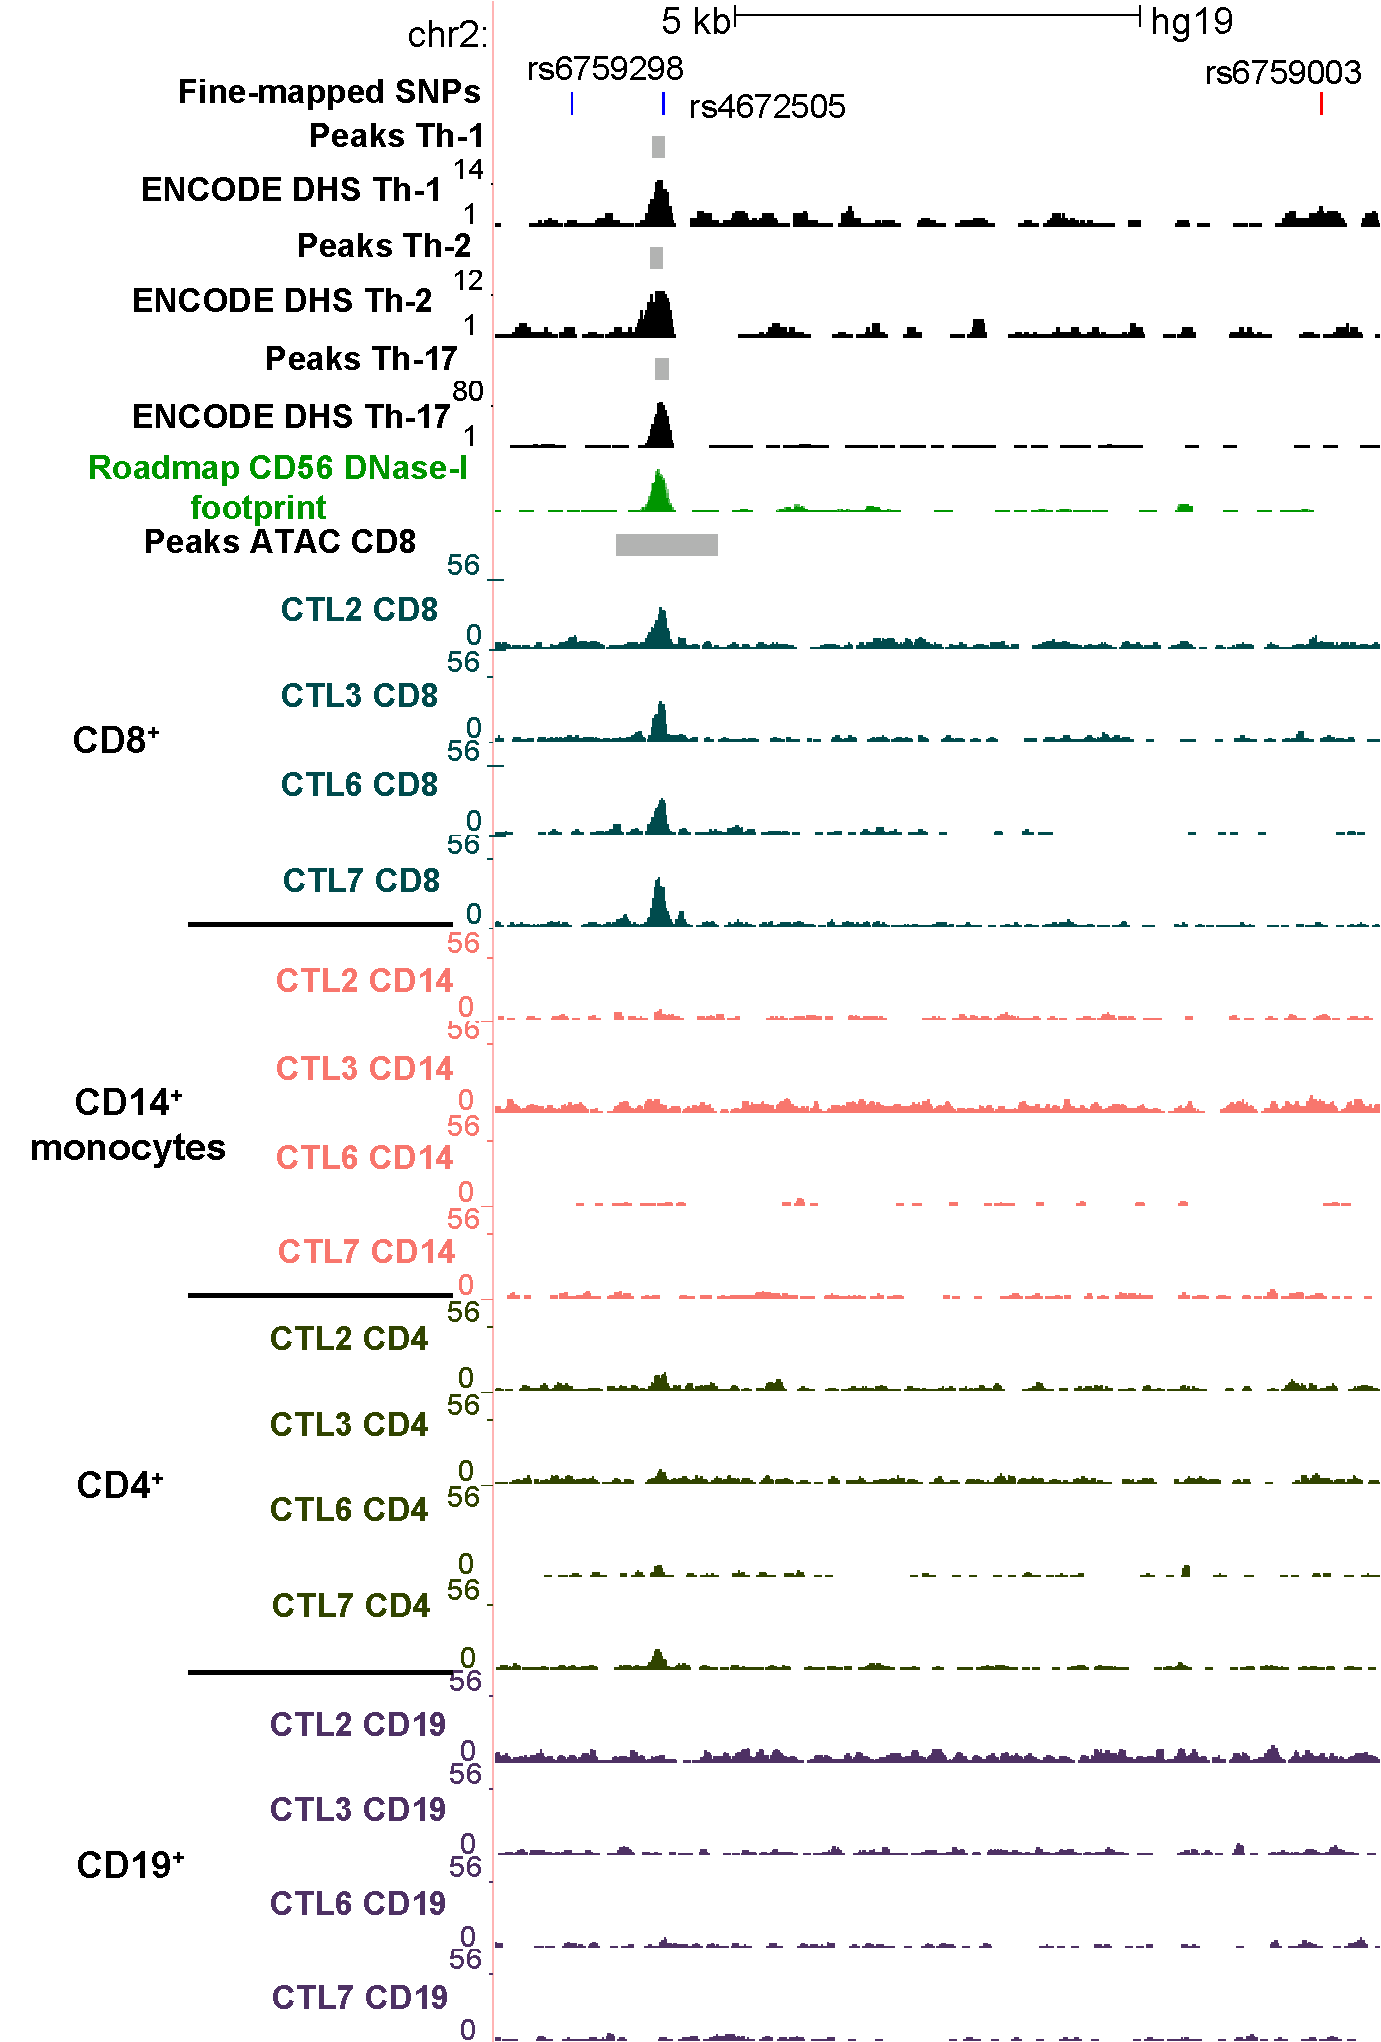
\includegraphics[width=\textwidth]{./Results2/pdfs/chr2p15_rs4672505_FM_all_cell_types_track_all_marks}
\caption{\textbf{}}
% The percentage sign indicated that the other subfig goes side by side
\end{subfigure}%
\begin{subfigure}[b]{0.45\textwidth}
\centering
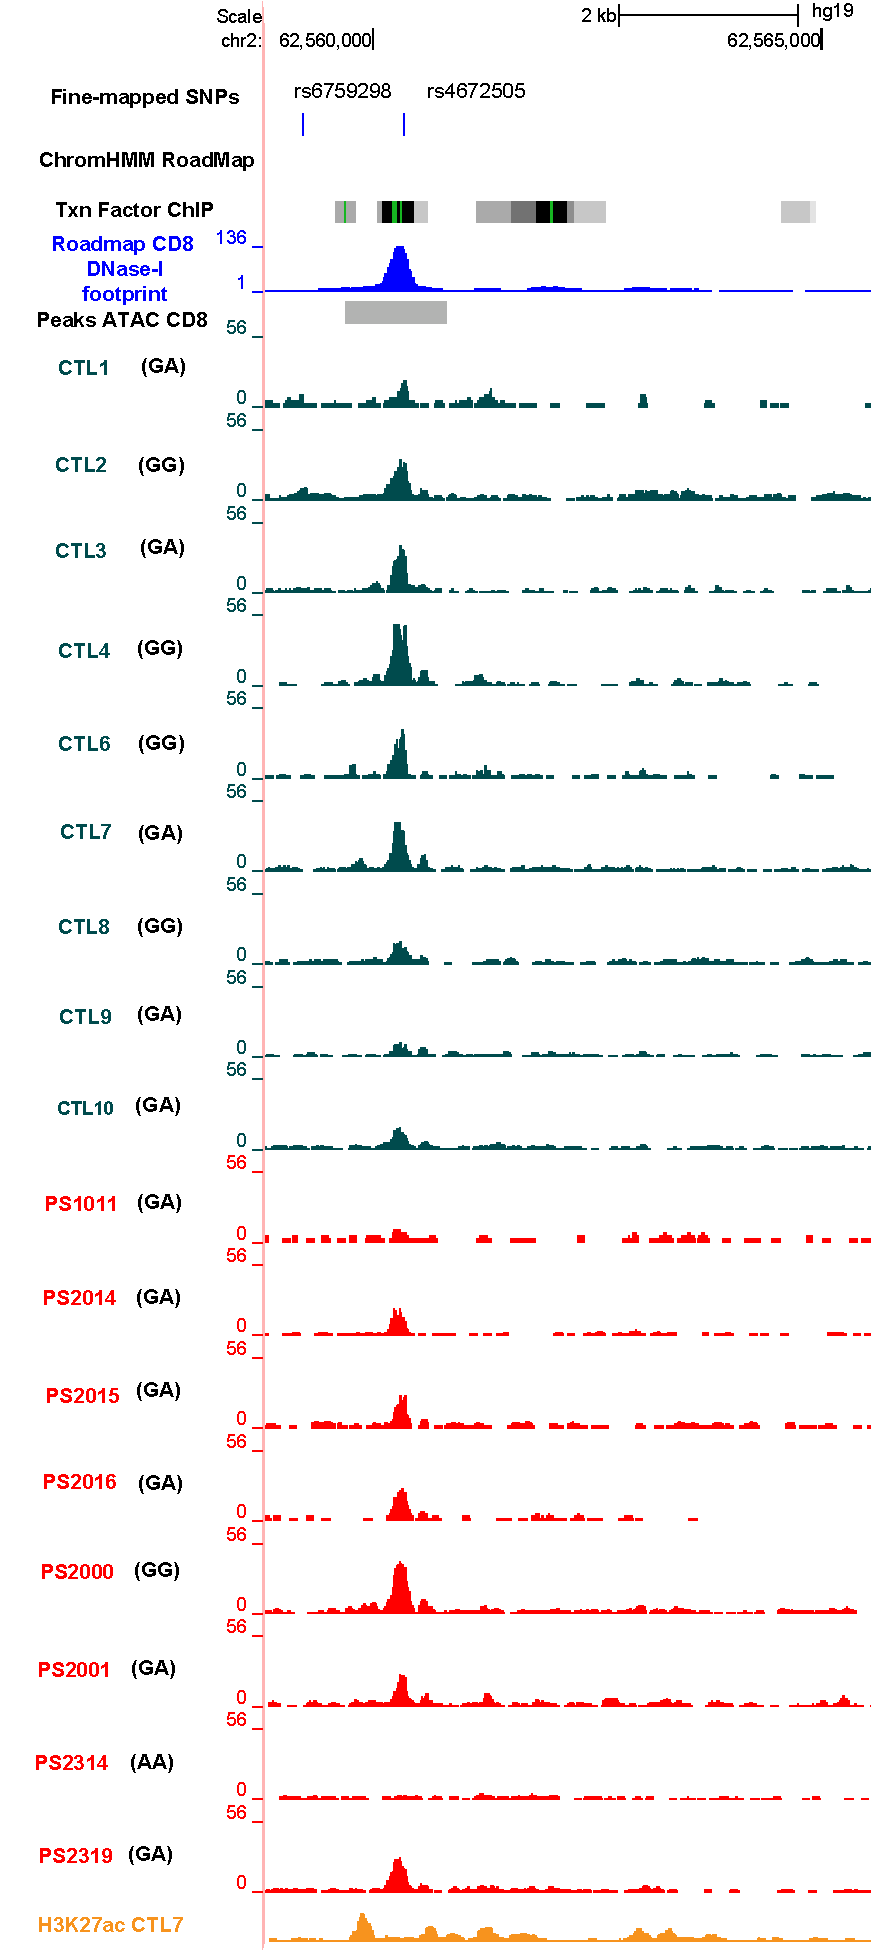
\includegraphics[width=\textwidth]{./Results2/pdfs/chr2p15_rs4672505_FM_CD8_track_all_marks}
\caption{\textbf{}}
\end{subfigure}
\caption[Epigenetic landscape at the location of the SNPs in the 95\% credible set for the chr2p15 GWAS psoriasis locus.]{\textbf{Epigenetic landscape at the location of the SNPs in the 95\% credible set for the chr2p15 GWAS psoriasis locus.} a) UCSC Genome Browser view illustrating normalised read density for in-house ATAC an a number of other publicly available epigenetic data (DHS, DNAse-I footprint, chromatin segmentation map) (y-axis) at the location of the three SNPs (rs6759298, rs4672505 and rs6759003) (x-axis) from the 95\% credible set obtained in the fine-mapping analysis of the chr2p15 GWAS association in AS. Representative ATAC data from the same four controls in the cohort and the four cell types included in this study are shown. b) UCSC Genome Browser view illustrating the normalised read density for tCD8$^+$ ATAC (x-axis) generated in psoriasis patients and healthy controls, in-house H3K27ac ChIPm, ENCODE TF ChIP-seq and DNase-I fooprint (y-axis) at the location of the SNP rs4672505 (y-axis). For each of the patients and controls of the cohort the Sanger sequencing genotype of rs4672505 is included.}
\label{figure:ATAC_PS_CTL_chr2p15_rs4672505}
\end{figure} 


For example, PS2314 and CTL1 showed no ATAC signal at this location when compared to PS2000 and CTL4. Integration with publicly available ENCODE DHS data also revealed accessible chromatin at rs4672505 in Th-1, Th-2 and Th-17 cells from ENCODE (Figure \ref{figure:ATAC_PS_CTL_chr2p15_rs4672505} a). Although this region was tagged as quiescent according to the tCD8$^+$ chromatin segmentation, Epigenome Roadmap primary tCD8$^+$ DNase-I digital genomic footprinting signal was found to overlap with the location of rs4672505 and the in-house ATAC peak (Figure \ref{figure:ATAC_PS_CTL_chr2p15_rs4672505} b), and may suggest a putative \textit{cis}-regulatory role for this region. The absence of histone marks and chromatin accessibility leading to annotation of this chromatin segment as quiescent by the Epigenome Roadmap could be explained by the variability across individuals found at this location. For example, H3K27ac data generated in cohort 1B demonstrated modest signal enrichment in CTL7, which also presented accessible chromatin at rs4672505; however no enrichment was detected for PS2314 (Figure \ref{figure:ATAC_PS_CTL_chr2p15_rs4672505} b). Regarding TFs, ENCODE ChIP-seq experimental data from GM12878 showed binding for RUNX3, a psoriasis and AS GWAS associated gene, with nominal association also in the PsA Immunochip GWAS study. Importantly, RUNX3 together with a number of TFs is involved in CD8$^+$ cell differentiation \parencite{Wong2011}. Further investigation using \textit{in silico} TFBS prediction, such as PROMO \parencite{Messeguer2002}, and ENCODE genomic DNase-I footprint in GM128778 predicted STAT1 binding at rs4672505. Altogether, integration of ATAC and publicly available epigenetic data indicated that rs4672505 was the most likely variant, amongst the three fine-mapped SNPs included in the 95\% credible set, to have a functional role explaining the association of chr2p15 with psoriasis risk.

% Not sure where to include the methyl QTLs

\subsubsection{Allele-dependent chromatin accessibility and allelic imbalance using ATAC reads at rs4672505}
The genotype of each individual at the rs4672505 SNP was characterised using Sanger sequencing. Amongst the eighteen samples (ten controls and eight psoriasis patients), one (PS2314) was homozygous for the risk allele (A, MAF=0.43), eleven were heterozygous and six were homozygous for the protective allele (G) (Figure \ref{figure:ATAC_PS_CTL_chr2p15_rs4672505} b genotypes in brackets). Interestingly, PS2314, the only homozygous individual for the risk allele, showed complete absence of the peak at rs4672505. In order to further investigate the role of rs4672505 genotype in the variability of chromatin accessibility across individuals, the normalised read counts retrieved at the chr2:62,559,749-62,561,442 ML\_CD8 peak were used as the dependent variable in linear model analysis based on rs4672505 genotype, using batch as a covariate. 



\begin{figure}[htbp]
\centering
\begin{subfigure}{0.45\textwidth}
\centering
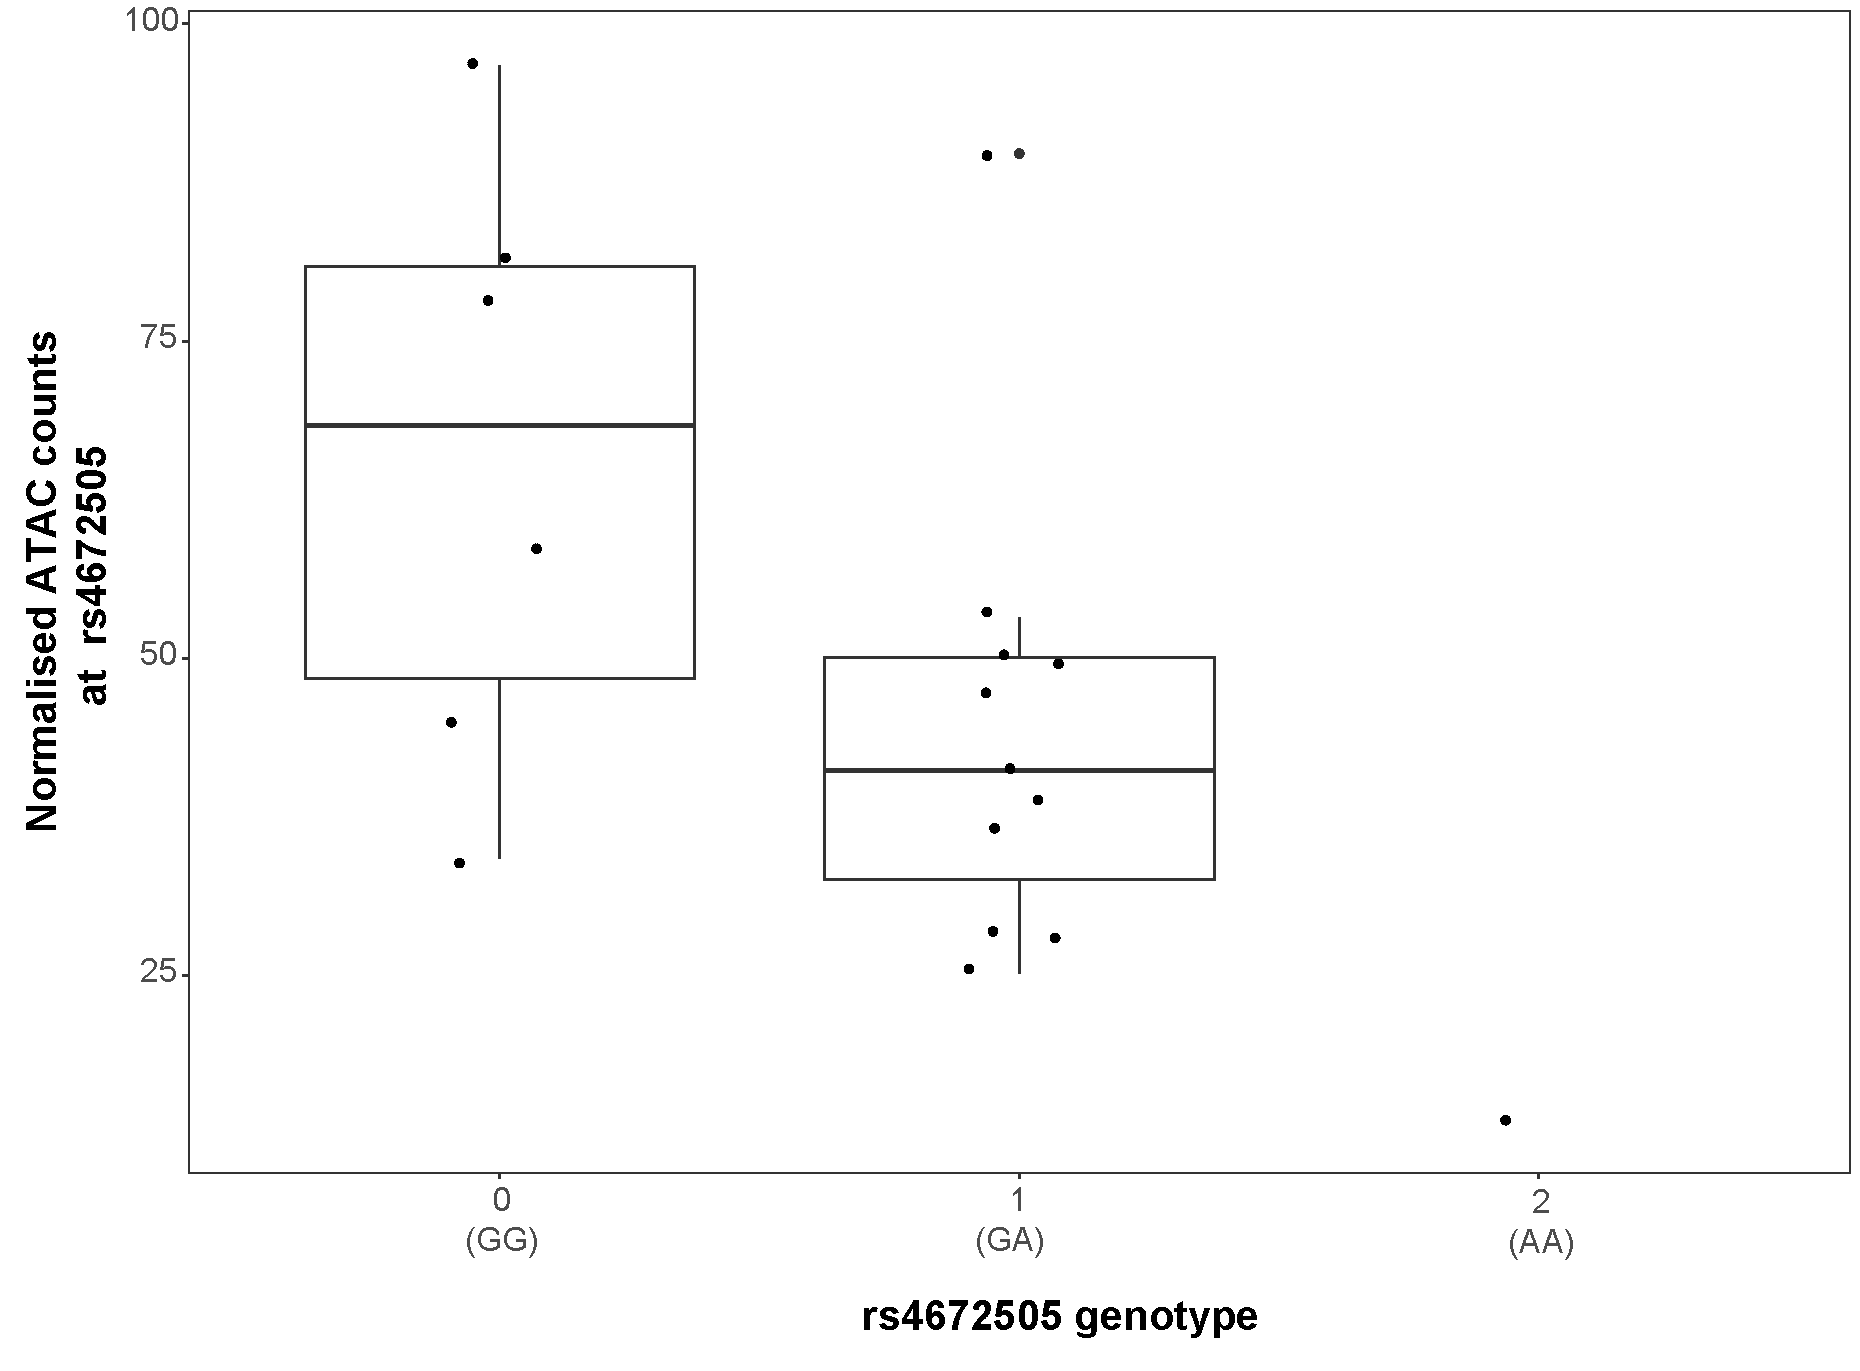
\includegraphics[width=\textwidth]{./Results2/pdfs/ATAC_caQTL_CD8_final}
\caption{\textbf{}}
% The percentage sign indicated that the other subfig goes side by side
\end{subfigure}%
\begin{subfigure}{0.45\textwidth}
\centering
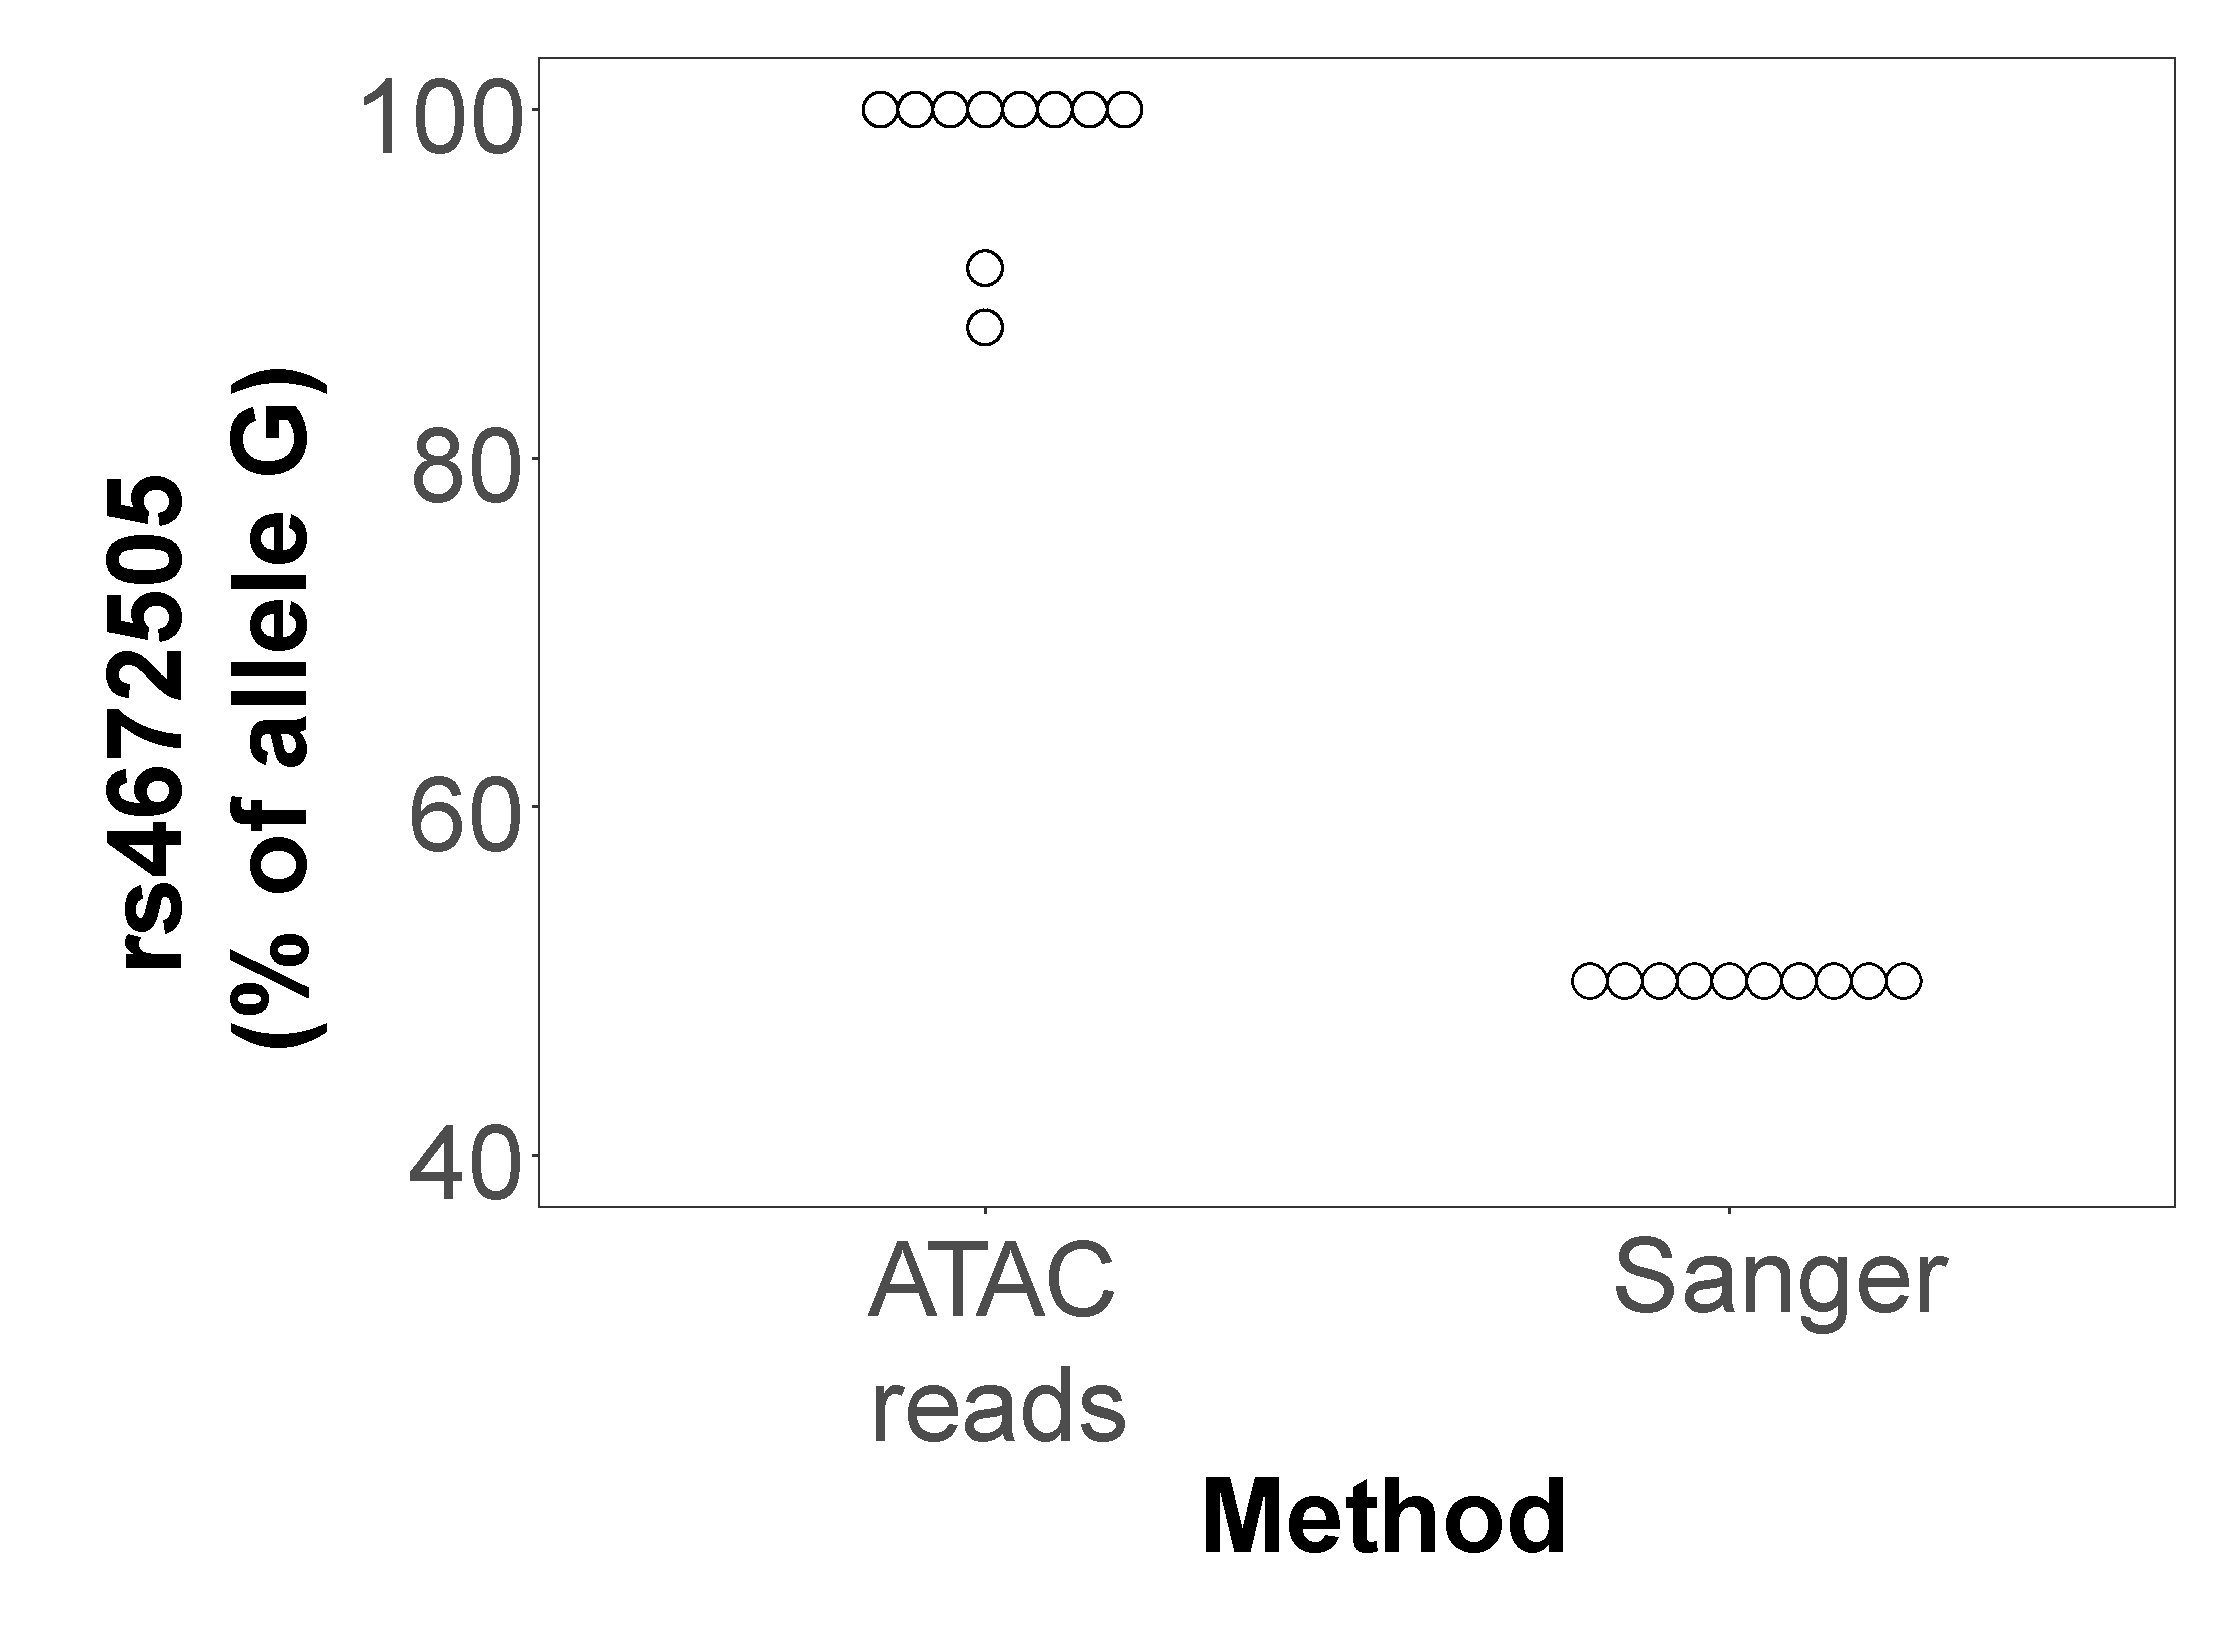
\includegraphics[width=\textwidth]{./Results2/pdfs/chr2p15_rs4672505_allelic_imbalance_CD8_final}
\caption{\textbf{}}
\end{subfigure}
\caption[Effect of rs4672505 genotype in tCD8$^+$ cells chromatin accessibility at chr2:62,559,749-62,561,442.]{\textbf{Effect of rs4672505 genotype in tCD8$^+$ cells chromatin accessibility at chr2:62,559,749-62,561,442.} a) Boxplot illustrating the effect of the rs4672505 genotype in chromatin accessibility at the chr2:62,559,749-62,561,442 ATAC peak. Log$_2$ normalised ATAC counts adjusted for batch effect, also included as a covariate for the linear model, are plotted for each sample against the number of copies of the minor allele (G=0, AG=1, AA=2). b) Representation of the percentage of ATAC reads overlapping rs4672505 and mapping to the major allele (G) in comparison to the Sanger genotype results for the eleven heterozygous individuals at this SNP.}
\label{figure:ATAC_PS_CTL_caQTL_and_allelic_imbalance}
\end{figure} 
 
Significant negative correlation (pval=0.035) was found, suggesting allele-dependent chromatin accessibility (Figure \ref{figure:ATAC_PS_CTL_caQTL_and_allelic_imbalance} a). Furthermore, allelic imbalance for the ATAC reads at rs4672505 position was investigated on those individuals identified as heterozygous by Sanger sequencing and for which 50\% of the ATAC reads were expected to map to each of the alleles. This analysis demonstrated a larger percentage of ATAC reads (greater than the expected 50\%) preferentially tagging the protective allele G (Figure \ref{figure:ATAC_PS_CTL_caQTL_and_allelic_imbalance} b). This finding was not driven by mapping bias, since A was the reference allele in the hg19 build used to map the ATAC data. Overall, these results showed a tendency towards greater chromatin accessibility in presence of the fine-mapped protective allele rs4672505(G) at the chr2p15 locus.
 

\subsubsection{Potential regulatory role of rs4672505 in the expression of B3GNT2}
As previously mentioned, one of the issues with intergenic GWAs signals is the difficulty in determining the gene they may be having an effect on through regulation of gene expression. rs4672505 is located 140Kb downstream of the \textit{B3GNT2} gene and 150Kb upstream of \textit{TMEM1}. Publicly available promoter capture data from Javierre \textit{et al.} 2016 in tCD8$^+$ revealed a genome-wide significant interaction (CHiCAGO score=7.67) between a region containing rs6759298 and rs4672505 and the promoter of the \textit{B3GNT2} gene (Figure \ref{figure:RNA_chromatin_interaction_B3GNT2} a). 

\begin{figure}[htbp]
\centering
\begin{subfigure}{0.5\textwidth}
\centering
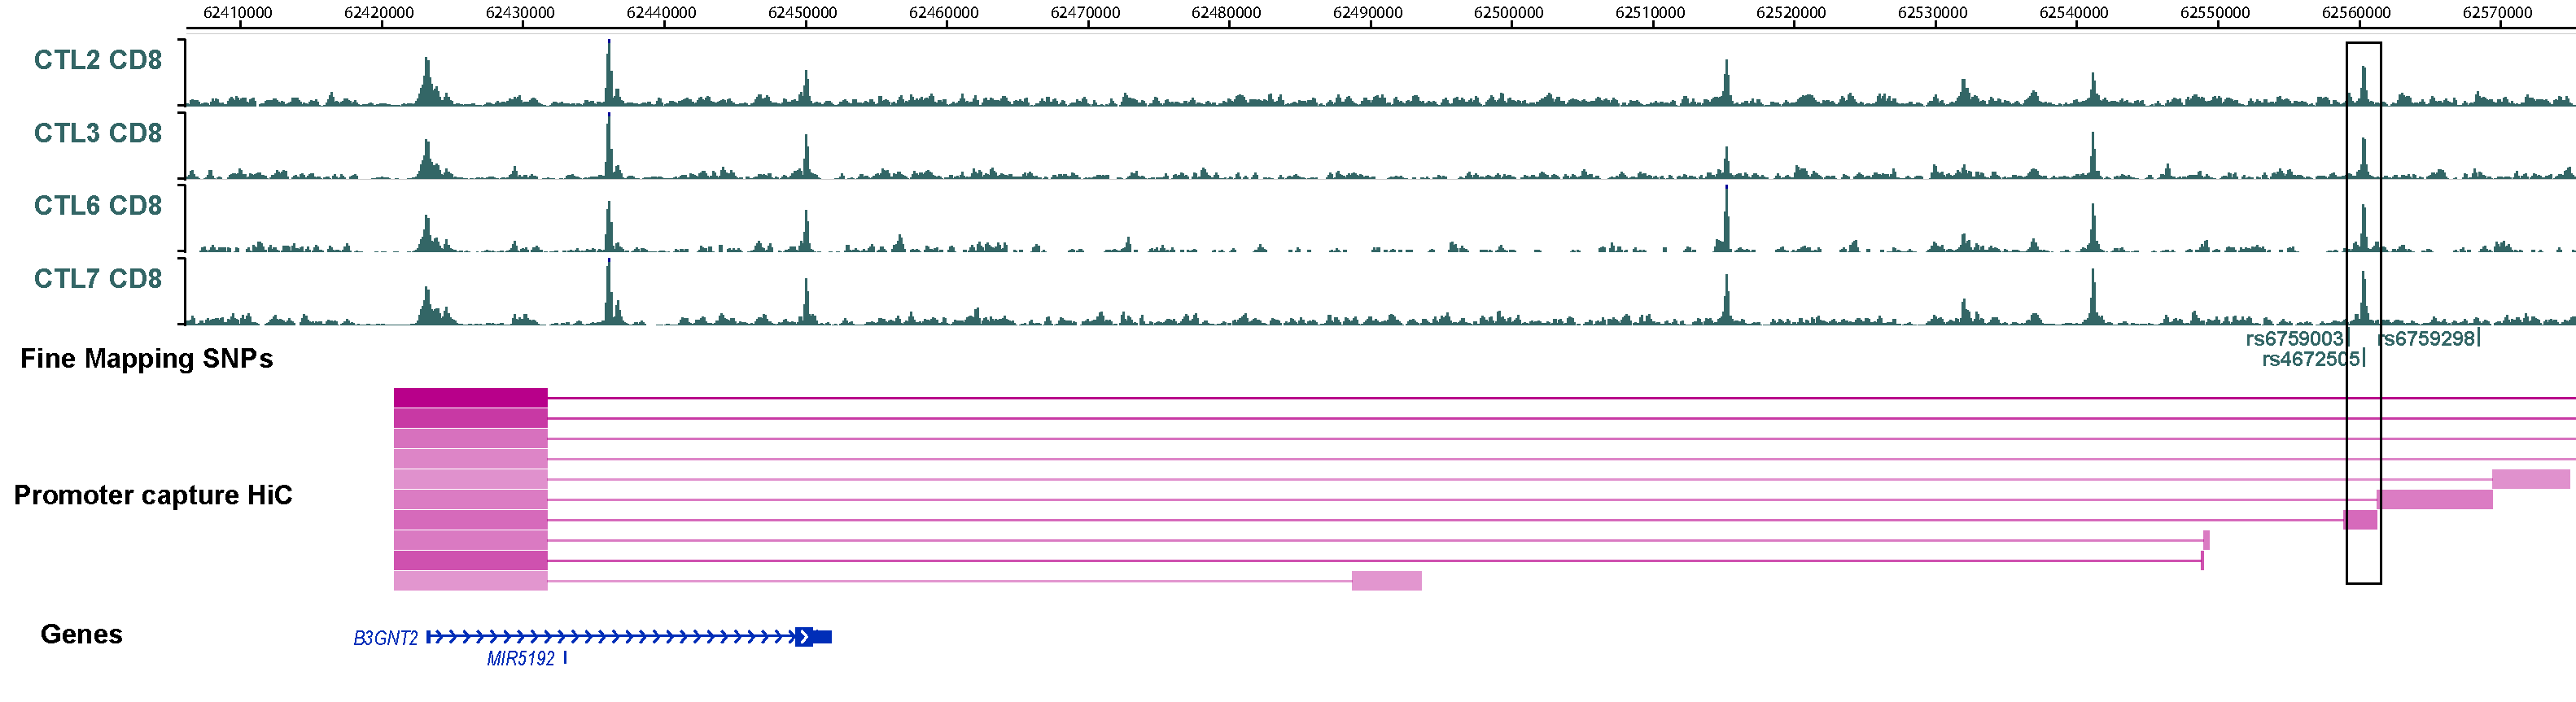
\includegraphics[width=\textwidth]{./Results2/pdfs/B3GNT2_HiCi_WASHU_track}
\caption{\textbf{}}
% The percentage sign indicated that the other subfig goes side by side
\end{subfigure}
\begin{subfigure}{0.5\textwidth}
\centering
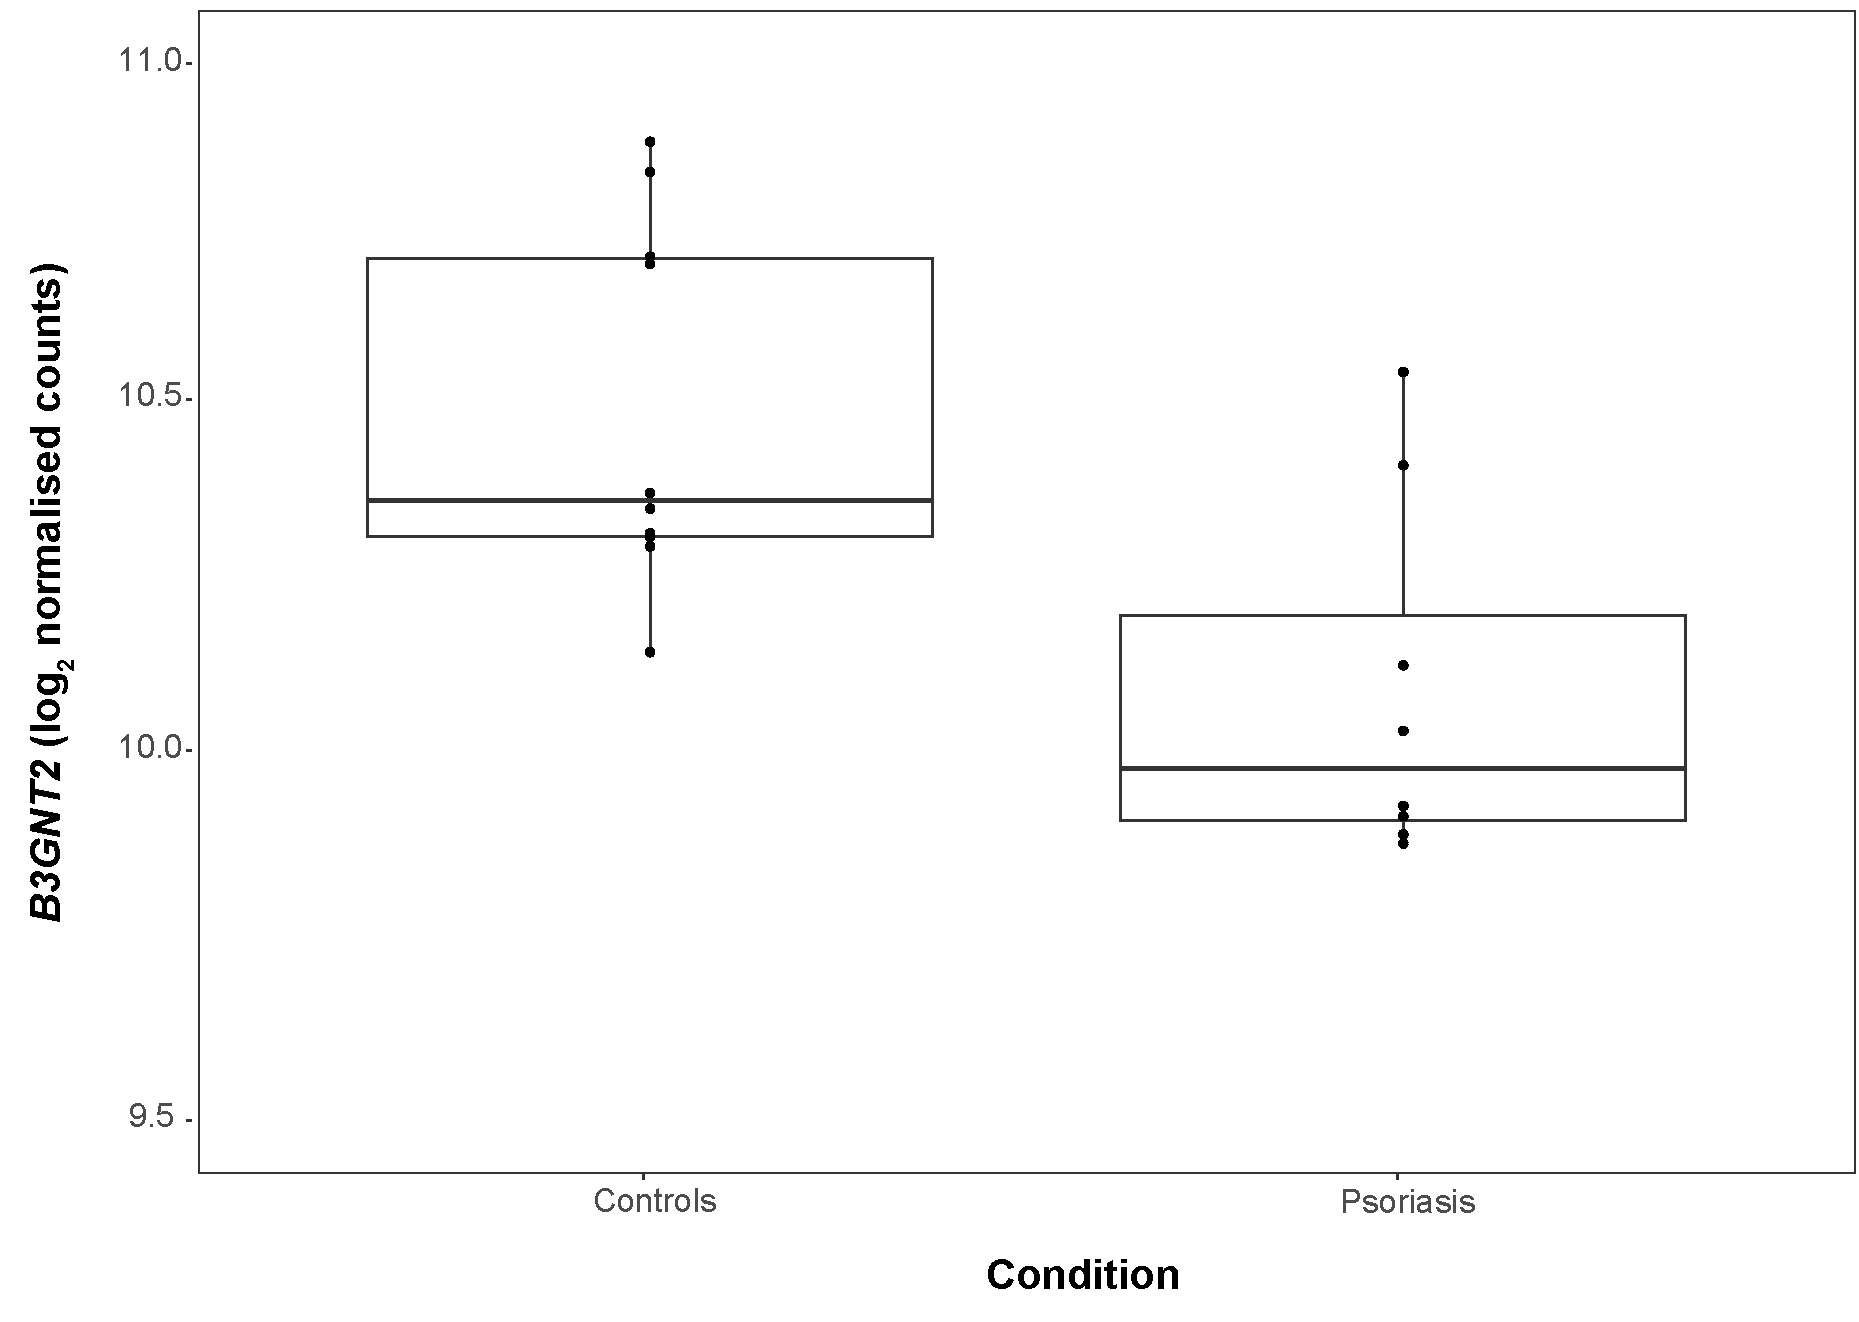
\includegraphics[width=\textwidth]{./Results2/pdfs/RNA_PS_CTL_B3GNT2_expression_CD8}
\caption{\textbf{}}
\end{subfigure}
\caption[Potential role of rs4672505 in regulating \textit{B3GNT2} gene expression.]{\textbf{Potential role of rs4672505 in regulating \textit{B3GNT2} gene expression.} a) WASHU Genome Browser track showing in tCD8$^+$ cells normalised ATAC read density in four of the healthy controls, the location of the three SNPs of the 95\% credible set and the promoter capture HiC data depicting the regions interacting with the bait at the \textit{B3GNT2} promoter. b) Boxplot illustrating the \textit{B3GNT2} log$_2$ normalised RNA-seq counts adjusted for batch effect in the psoriasis and healthy control groups.}
\label{figure:RNA_chromatin_interaction_B3GNT2}
\end{figure} 



This interaction was not found in any of the additional sixteen human primary hematopoietic cell included in the study. Moreover, no upstream interaction with \textit{TMEM1} promoter was identified. Investigation of the publicly available T cell eQTL dataset from Kasela \textit{et al.} and Raj \textit{et al.} did not show a significant eQTL for this SNPs or SNPs in high LD (r$^2$$>$0.8) either in tCD8$^+$ or tCD4$^+$ \parencite{Raj2014,Kasela2017}. Similarly, no eQTL effect of rs4672505 was found in unstimulated or stimulated CD14$^+$ monocytes \parencite{Fairfax2014}. Conversely, whole blood eQTL study from Jansen and colleagues revealed a significant \textit{cis}-eQTL (FDR=1.34x10$^-5$) with moderate effect size ($\beta$=-0.16) for the minor allele \parencite{Jansen2017}. In terms of gene expression, significant (FDR$<$0.05) moderate down-regulation was observed in psoriasis patients when compared to controls in tCD8$^+$ (Figure \ref{figure:RNA_chromatin_interaction_B3GNT2} b) and CD19$^+$ cells (-log$_2$FC=-0.317 and -log$_2$FC=-0.317, respectively). \textit{B3GNT2} was not significantly dysregulated in lesional skin when compared to uninvolved. This data confirms dysregulation of \textit{B3GNT2} expression in psoriasis and may suggest a role for rs4672505 in the regulation of \textit{B3GNT2} expression in tCD8$^+$ only under certain conditions.  

%%%%%%%%%%%%%%%%%%%%%%%%%%%%%%%%%%%%%%%%%%%%%%%%%%
\section{Discussion}

\subsection{Chromatin accessibility and H3K27ac landscape in psoriasis immune cells}
Comparison of chromatin accessibility and H3K27ac histone modifications has revealed a small number of differential regions between patients and controls in the four cells types under study. For both epigenetic features, CD14$^+$ monocytes and tCD8$^+$ cells had the largest number of discrete changes. In ATAC, greater accessibility in tCD8$^+$ cells from patients compared to controls was found at two regions proximal to \textit{IL7R} and \textit{TNFSF11}, respectively, that also overlap FANTOM eRNA in the same cell type. Both genes are well known for having a pro-inflammatory effect and be involved in chronic inflammatory diseases. For example, \textit{TNFSF11} is downstream of the lead SNP for a CD risk locus, and its protein product RANKL was found to be overexpressed in epidermis from psoriasis patients, highlighting the role of this gene in the pathophysiology of psoriasis \parencite{Toberer2011}. 

Integration of the ATAC and H3K27ac ChIPm differential analysis only found one overlapping region at an intron of the \textit{DTD1} gene, which participates in initiation of DNA replication and is associated with aspirine-intolerance in asthmatics\parencite{Pasaje2011}. However, evidence of \textit{DTD1} involvement in chronic inflammation has yet not been reported. The lack of overlap between DARs and differentially H3K27ac modified regions might be expected given that chromatin accessibility is driven by the interaction between a number of histone modifications, TFs, and structural proteins, such as CTCF. 

The results in this chapter suggest that disease status does not involve global differences in chromatin accessibility and H3K27ac between patients and controls in the studied circulating immune cells. Recent similar studies performing ATAC in B cells from SLE patients and in AMD retina and retinal pigmented epithelium have revealed larger differences in the chromatin accessibility landscape between patients and controls \parencite{Scharer2016,Wang2018}. Similarly, H3K27ac mapping in mCD4$^+$ cells isolated from juvenile idiopathic arthritis SF found approximately one thousand differential enhancers when compared to healthy control circulating cells \parencite{Peeters2015}. Conversely only small differences were found when comparing mCD4$^+$ from PB of patients and controls, highlighting the specificity of the disease signature at the site of inflammation. Importantly, direct interrogation of the main cell type or tissue affected by inflammation in those studies would partly explain the more profound changes observed in the chromatin landscape compared to my study. Additionally, some differences will be driven by genotype, and by the nature of complex diseases different patients have different genetic backgrounds, with some variants also shared with control individuals. Thus it may be necessary to study changes in chromatin accessibility in the context of genotype and under exogenous inflammatory stimuli that may manifest those differences \parencite{Alasoo2018,Calderon2018}.

\subsection{Dysregulation of gene expression in psoriasis circulating immune cells}
Comparison of gene expression between psoriasis and healthy controls in a cell type specific manner identified larger numbers of DEGs compared to DARs or differential H3K27ac modifications. As for ATAC and ChIPm, CD14$^+$ monocytes and tCD8$^+$ cells showed the largest number of transcriptomic changes in disease. This may suggest greater relevance of these two cell types in the systemic “footprint” of psoriasis.   The more dysregulated gene expression in tCD8$^+$ compared to tCD4$^+$ may suggest that, as in skin, CD8$^+$ are the main effector cells upon induced-activation by CD4$^+$ cells \parencite{Nickoloff1999}. The importance of monocytes/macrophages in psoriasis has also been demonstrated by their presence in psoriatic skin where TNF-$\alpha$ production contributes towards maintenance of inflammation \parencite{Nickoloff2000,Wang2006}. 

The overlap of DEGs with previous studies comparing PBMCs from psoriasis patients was limited, probably due to many differences identified in my cell type specific analysis being masked by the admixture of cells as well as those studies using microarrays instead of RNA-seq \parencite{Lee2009,Coda2012}. Although those studies did not find specific enrichment for any pathway, Coda and colleagues identified some genes were associated with pathophysiological processes such as immune response, oxidative stress or apoptosis \parencite{Coda2012.}. 

The cell type specific analysis conducted in my thesis identified significant enrichment of relevant biological processes, including MAPK and IL-12 signalling, in the CD14$^+$ monocytes and tCD8$^+$ cells contrast. Interestingly, some of the well-known pro-inflammatory genes contributing to the enrichment of these pathways were down-regulated in psoriasis compared to controls. For example, \textit{MAP3K4} down-regulation in LPS stimulated PBMCs has been identified as an immune-suppressive feature in CD leading to reduced expression of the cytokine IL-1$\alpha$. In the IL-12 signalling pathway, leading to T cell proliferation and IFN-$\gamma$ production through activation of TFs from the STAT family, CD14$^+$ cells presented down-regulation of \textit{STAT4} and \textit{STAT5A} in psoriasis versus controls. Other member of the STAT family, such as \textit{STAT2}, was found to be down-regulated in psoriasis PBMCs and in AS monocyte-derived macrophages when compared to controls \parencite{Coda2012,Smith2008}. Monocytes do not express \textit{STAT4} in basal conditions but up-regulation follows IL-12, IL-18 and IFN-$\alpha$ stimulation \parencite{Frucht2000,Schindler2001}. STAT5 phosphorylation in monocytes is mainly induced by granulocyte macrophage-colony stimulating factor (GM-CSF) and promotes differentiation into macrophages. Interestingly, STAT5 downstream gene targets such as prostaglandin synthase 2 (\textit{COX2}) and \textit{IL-10} were not dysregulated in CD14$^+$ monocytes in my data. In other chronic inflammatory diseases such as T2D, persistent STAT5 phosphorylation has been found in circulating monocytes isolated from T2D upon GM-CSF \parencite{Litherland2005}. Further investigation to determine phosphorylated STAT4 and STAT5 protein abundance will be require to determine if the down-regulation at the transcript level observed in psoriasis CD14$^+$ monocytes is biologically relevant. In tCD8$^+$, expression of \textit{IFNG} a gene activated by the IL-12 signalling pathway, was down-regulated when compared to healthy controls. Down-regulation of \textit{IFNG} has previously been reported in unstimulated and stimulated macrophages derived from AS patients, in SF from SpA patients compared to RA and in a SpA rat model \parencite{Smith2008,Fert2014, }. This down-regulation was accompanied by an overall “inverse” transcriptional response of IFN-regulated genes, which was not seen in my data. Moreover, the reduced expression of \textit{IFNG} in knock-out mice has been shown to increase activation of the IL-23/IL-17 axis, which is pivotal in psoriasis pathogenesis \parencite{Canete2000,Chu2007}. Therefore, down-regulation of \textit{IFNG} may actually result in a pro-inflammatory effect. 

In tCD8$^+$ specifically, DEGs showed significant enrichment for three very relevant pathophysiological pathways in psoriasis: NF-$\kappa$B, TNF and chemokine signaling. Important cross-talk between the NF-$\kappa$B and TNF signaling pathway was observed, with a number of dysregulated genes contributing to both. Interestingly, the enrichment of these pathways involved up-regulation of pro-inflammatory genes (e.g \textit{ATF2}, \textit{ATF4}, \textit{RELA}, \textit{RELB}) but also increased expression of well-characterised immunoregulatory genes. These included \textit{NFKBIA} and \textit{TNFAIP3}, also up-regulated in CD14$^+$ monocytes and CD4$^+$ cells respectively, and both associated with psoriasis GWAS signals.  Polymorphisms within \textit{TNFAIP3} or in its vicinity have also been associated with a number of chronic inflammatory diseases including MS, RA, SLE and T1D \parencite{Vereecke2011}. \textit{NFKBIA} codes for I$\kappa$B$\alpha$ which inhibits NF-$\kappa$B by binding it and preventing translocation to the nucleus. \textit{TNFAIP3} codes for the zinc finger protein and ubiqitin-editing enzyme A20, and is up-regulated in the presence of inflammation and NF-$\kappa$B activation in order both to inhibit the NF-$\kappa$B TNF-mediated response and promote return to homeostasis. Either \textit{NFKBIA} or \textit{TNFAIP3} were found to be dysregulated in psoriasis PBMCs by Coda \textit{et al.}, Lee \textit{et al.} and Mesko \textit{et al.} or in PBMCs from PsA patients versus controls \parencite{Dolcino2015}. Interestingly, qPCR analysis in PBMCs from mild (PASI$<$4.84) and severe (PASI$>$4.84) psoriasis vulgaris revealed a significant negative correlation between \textit{TNFAIP3} expression and disease severity \parencite{Jiang2012}. Furthermore, this study also demonstrated that in the mild group of patients but not in the severe \textit{TNFAIP3} expression was down-regulated when compared to healthy control PBMCs. This is in line with my findings with the caveat that all patients from my cohort would be classified as severe by Jian \textit{et al.}. Altogether, the up-regulated expression of \textit{TNFAIP3} and \textit{NFKBIA} compared to healthy controls may not be unexpected as it reflects a persistent inflammatory stimuli in psoriasis PB and a mechanism that limits the systemic inflammatory response to some extent \parencite{Idel2003}. 

Of interest was also the up-regulation of the chemokine receptor \textit{CCR10} in tCD8$^+$ cells from psoriasis patients. In circulation, expression of \textit{CCR10} is restricted to a subset of circulating mCD4$^+$ and mCD8$^+$ T cells expressing the cutaneous lymphocyte-associated antigen (CLA), and preferentially recruited to cutaneous sites of inflammation \parencite{Hudak2002}. Indeed, an increase of CCR10$^+$ infiltrated T lymphocytes in psoriatic skin, where KCs express \textit{CCR10} ligand \textit{CCL27}, has been demonstrated \parencite{Homey2002}. The up-regulation of \textit{CCR10} in my data could potentially suggest an increase of mCD8$^+$ CCR10$^+$ cells ready to migrate into the skin lesions. Moreover, correlation between the frequency of CTLA$^+$ CD8$^+$ cells and disease severity measured by PASI score has been found \parencite{Sigmundsdottir2001}. Overall, these data have revealed dysregulation between psoriasis patients and controls for relevant immune genes showing pro- and anti-inflammatory effects in circulating immune cells. Although down-regulation of pro-inflammatory genes and up-regulation of anti-inflammatory genes has been detected, understanding the overall effect of those interactions in the inflammatory response requires further investigation. 




\subsection{Correlation between changes in chromatin accessibility and gene expression}
In this chapter, greater changes in gene expression have been identified compared to chromatin accessibility. Strikingly, in tCD8$^+$ cells, 687 transcripts were differentially expressed between psoriasis and healthy controls but only 55 regions showed differential chromatin accessibility when performing the same contrast and only six of the 687 were proximal to a DAR. Correlation between chromatin accessibility measured by ATAC and gene expression has been reported to some extent in a number of studies, with limitations in establishing relationships between enhancer regions and the regulated target \parencite{Ackermann2016,Wang2018}.

Chromatin accessibility shows the current functional landscape of the genome and will have some correlation with the current transcriptional state of the cell. The RNA transcripts however will be both a view of the current transcription and previous changes in transcription as well as other events related to RNA turnover and lncRNAs and microRNAs interactions and regulatory processes at the RNA level. As such, the larger changes in gene expression compared to chromatin accessibility here could bedue to a non-direct relationship between chromatin accessibility and transcripts. Also, the discrepancy may also be due to different sensitivities from the ATAC assay to identify changes in chromatin accessibility and that of the RNA-seq analysis.
An example of a relevant DEG nearby a DAR was \textit{TIAM1}, with increased chromatin accessibility and gene expression in psoriasis tCD8$^+$ cells compared to healthy controls. \textit{TIAM1} is involved in IL-17 expression and cell migration into the inflamed tissue \parencite{Kurdi2016, Gerard2009}.  However, no eQTL or chromatin conformation data in this cell type has been found to formally establish a link between the region harbouring this DAR and \textit{TIAM1} expression.


\subsection{Trancriptomic profiles in lesional and uninvolved psoriatic epidermis}
Investigation of differences in the transcriptomic profile between paired lesional and uninvolved skin was conducted for three psoriasis patients in my cohort. Most previous transcriptional studies in psoriasis have used full thickness skin biopsies, formed of a mix of cell types including fibroblast, adipocytes, KCs from the epidermis and dermis and infiltrated immune cells. A study from Ahn and colleagues demonstrated large differences in gene expression between whole biopsies and FACS-isolated KCs, which may be masking KC-specific pathophysiological differences in many previous studies using psoriasis skin biopsies \parencite{Ahn2016}. In this chapter, RNA-seq was conducted on epidermal sheets isolated from whole biopsies and a total of 1,227 DEGs were identified. 
Comparison with the Tervaniemi \textit{et al.} study contrasting gene expression between lesional and uninvolved epidermis split biopsies, mainly formed by epidermis, revealed an overlap of only 359 out of the 1,227 DEGs detected in my data (12.1\% of Tervaniemi \textit{et al.} DEGs). Interestingly, the overlap with the Tsoi \textit{et al.} study using whole biopsies was similar (505, 13.1\% of Tsoi \textit{et al.} DEGs) and only 5 genes had opposite direction of change, in contrast with the 75 showing discrepancies with Tervaniemi’s study.  The similar percentage overlap with the Tsoi study despite the different source material could simply be the result of greater power in that study. 


Genes consistently up-regulated across the three studies included genes from the \textit{S100A} family. The \textit{S100} family are located in the chr1p21 locus, which harbours genes involved in KCs differentiation, act as calcium sensors and may also have a chemotactic effect \parencite{Eckert2004}. In particular, \textit{S100A9} and \textit{S100A12} undergo up-regulation in psoriasis \parencite{Broome2003}, with the latter involved in the T cell proliferative response and IFN-$\gamma$ and IL-2 production \parencite{Moser2007}.  \textit{LCE3B}, also at the chr1p21 locus, was also upregulated in lesional skin compared to uninvolved in all three studies. \textit{LCE3B/C}\_\textit{del}, a psoriasis GWAS association, is found in approximately 60 to 70\% of European psoriasis patients \parencite{Cid2009}. As explained in Chapter \ref{ch:Intro}, \textit{LCE} gene expression is induced upon disruption of the skin barrier, and expression of \textit{LCE3B} and \textit{LCE3D} has been only detected in lesional but not uninvolved psoriatic skin of heterozygous individuals \parencite{Cid2009,Bergboer2011}. This suggests that the three psoriasis patients in the study are heterozygous for the deletion.


Pathway enrichment analysis for the DEGs between lesional and uninvolved skin revealed a number of relevant biological processes for psoriasis pathophysiology. These highlighted alterations in cell cycle and metabolic processes, including amino acid metabolism, glycolysis, and hypoxia (HIF-I signalling), which had been identified in other studies performing DGE analysis between lesional and uninvolved skin or genome-wide pathway analysis \parencite{Coda2012, Gudjonsson2010,Aterido2016, Tervaniemi2016}. The enrichment of the HIF-I pathway in psoriasis is the result of an increased rate of cell proliferation leading to hypoxia and angiogenesis.  Up-regulation of the hypoxia-inducible TFs HIF-1$\alpha$ and HIF-2$\alpha$ has been found in lesional skin, correlated with an increase in \textit{VEGF} transcript levels, a gene regulated by HIFs that mediates pathological angiogenesis also characteristic of psoriasis \parencite{Rosenberg2007}. No correlation was observed between \textit{HIFA} and \textit{VEGF} in my data, likely due to the small sample size. Moreover, HIF-I signalling is also involved in regulating Th-17/Treg ratios and therefore in perpetuation and termination of the immune response \parencite{Dang2013}. 

Immune-related pathway enrichment were also found in my analysis, including Th-17, IL-12, cytokine-cytokine and NOD-like signalling. Interestingly, NOD-like signalling was found to be enriched in DEGs between lesional and uninvolved skin in a contemporary study by Tervaniemi and colleagues \parencite{Tervaniemi2016}. Tervaniemi mainly attributed this novel pathway to the greater sensitivity of RNA-seq compared to microarrays to detect changes in gene expression for genes involved in this pathway. The fact that Tsoi \textit{et al.} also used RNA-seq and did not show enrichment for NOD-like signalling is likely due to the type of biopsy, highlighting the value of studying epidermis instead of full thickness skin to uncover dysregulation of functional pathways in KCs. NOD-like signalling involves signal transduction by NOD-like receptors, a type of pattern-recognition receptors, which can recruit and activate caspases into the inflammasomes or trigger inflammation through NF-$\kappa$B and MAPK.  Amongst the genes contributing to this patway \textit{CARD6}, \textit{IFI16}, \textit{NOD2} and \textit{NLRX1} overlapped with Tervaniemi’s data and showed up-regulation in both. Notably, polymorphisms in \textit{NOD2} have been linked to inflammatory diseases such as CD, atopic eczema and arthritis and potentially with psoriasis and PsA \parencite{Zhong2013,Zhu2012}.

Lastly, PPAR signaling appeared as a pathway linking metabolic and innate immunity dysregulation in psoriasis. PPARs are TFs activated by fatty acid signaling with an anti-inflammatory role in the development of metabolic diseases and chronic inflammation such as RA \parencite{Straus2007,Ji2001}. Similar to my study, \textit{PPARD} has been found to be up-regulated in psoriatic lesional skin, and molecular studies have demonstrated a role of this PPAR  in KC hyperproliferation through induction of heparin-binding EGF-like growth factor (HB-EGF) \parencite{Romanowska2008}.

\subsection{LncRNAs in psoriasis}
In addition to protein coding genes, the transcriptomic comparisons conducted in my study revealed dysregulation of a number of lncRNAs. The role of lncRNAs has been studied in RA, SLE, AS, and PsA \parencite{Muller2014,Shi2014,Zhang2017, Dolcino2018} but no study has been conducted to identify differentially lncRNAs in a cell type-specific manner in psoriasis PB. Conversely, several studies have contrasted lncRNAs in lesional compared to uninvolved or healthy skin \parencite{Li2014, Ahn2016, Gupta2016, Tsoi2015}. My analysis in circulating immune cells revealed the largest number of differentially expressed lncRNAs in CD14$^+$ monocytes and tCD8$^+$ (28 and 31, respectively for FDR$<$0.05) when comparing psoriasis patients to healthy controls. In skin, 46 lncRNAs showed dysregulated expression between lesional and uninvolved skin (FDR$<$0.05), and 24 had also been reported by Tsoi \textit{et al.}, 2015.    

Characterisation of lncRNA biological function is a developing field, which represents a limitation when interpreting these results \parencite{Uszczynska-Ratajczak2018}.  Some of the well-characterised dysregulated lncRNAs have a role in the immune response. For example, in psoriasis CD14$^+$ monocytes the up-regulation of \textit{HOTAIRM1} corresponded to down-regulation of the predicted target gene \textit{USP1}, unlike in Dolcino \textit{et al.} 2018. \textit{UPF1} is involved in nonsense-mediated decay and in partnership with the monocyte chemotactic protein-1-induced protein-1 (\textit{MCPIP1}) gene drives degradation of inflammation-related mRNAs to ensure maintenance of homeostasis \parencite{Mino2015}. Down-regulation of \textit{UPF1} in psoriasis CD14$^+$ monocytes may suggest impairment of this homeostatic mechanism, contributing to disease pathophysiology in this cell type. Another example of a relevant lncRNA up-regulated in CD14$^+$ monocytes was \textit{NEAT1}, which has also shown up-regulation in SLE CD14$^+$ monocytes. Knock-down demonstrated impairment of TLR4 signalling and down-regulation of inflammatory genes including IL-6 and CXCL10 \parencite{Zhang2016}. However, neither of those two genes was dysregulated in my study in this cell type. 


Interestingly, \textit{MIR146A} was differentially expressed between lesional and uninvolved skin but also when comparing psoriasis tCD8$^+$ to healthy controls. Molecular studies have suggested a role for miR-146a as a negative regulator of the TLR4 pathway through inhibition of TNF associated factor 6 (\textit{TRAF6}) and IL-1 receptor-associated kinase 1 (\textit{IRAK1}) expression \parencite{Taganov2006}. TRAF6 and IRAK1 are adaptor molecules involved in the activation of kinases that eventually lead to translocation of NF-$\kappa$B and AP-1 into the nucleus. Opposite direction of change was observed in the two comparisons here. The up-regulation of \textit{MIR146A} in psoriasis tCD8$^+$ compared to controls is in line with findings in serum from SLE and early RA patients \parencite{Wang2012,Filkova}. In contrast, trancriptomic studies using PBMCs from plaque psoriasis and also similar studies in RA (including PBMCs, SFMCs and CD4$^+$ isolated from both tissues, amongst others) have reported increased levels of miR-146a in patients when compared to controls \parencite{Ele-Refaei2015,Churov2015}. Conversely, the up-regulation of \textit{MIR146A} expression in lesional epidermis compared to uninvolved has been observed in other studies, and was also shown to be increased in lesional skin versus healthy biopsies \parencite{Lerman2014, Tsoi2015,Li2014}. One of the predicted gene targets of miR-146a, the TF \textit{NFAT5} was down-regulated in lesional skin and showed significant negative correlation with \textit{MIR146A} expression. Interestingly, up-regulation of \textit{NFAT5} has been reported in RA SF and has a role in mediating angiogenesis and proliferation of synoviocytes \parencite{Han2017}. Although in disagreement with the observations in PBMCs, the down-regulation of miR-146a levels in tCD8$^+$ cells would support failure of one of the check-points controlling sustained inflammation and the subsequent pathophysiological implications. In contrast, the up-regulation observed in lesional skin would not fit directly with the dysregulated inflammatory response in skin. 


Other dysregulated non-coding RNAs in lesional epidermis relevant to psoriasis pathophysiology were \textit{HG19} and \textit{MIR31HG}, down- and up-regulated respectively in my data. Both non-coding RNAs were also differentially expressed in Tsoi \textit{et al.}, 2015 and are involved in KC differentiation. In particular, silencing miR-31hg in the KC immortal cell line HaCaT induced cell cycle arrest and inhibited cell proliferation, consistent with two characteristic aspects dysregulated in psoriatic KCs \parencite{Gao2018}.
Overall, the lncRNA differential analysis conducted in this chapter gives an overview of dysregulation in blood and skin of psoriasis patients. A more comprehensive analysis could be performed to identify putative targets for all the identified lncRNAs. Those interactions could then be used to identify relevant biological processes through network and pathway analysis using only those dysregulated lncRNAs matching dysregulated target genes, similarly to the strategy used by Dolcino \textit{et al.,} 2018. However, such an analysis would likely require increased sample size to be appropriately powered.

\subsection{Differences in transcriptional dysregulation in blood and skin}
Comparison of the dysregulated genes in circulating immune cells and in psoriatic skin revealed very limited overlap.  Overall, FCs in the epidermis appeared to be larger than in circulating immune cells, likely due to a more profound pro-inflammatory environment driving gene expression changes in skin. CD14$^+$ monocytes and tCD8$^+$ cells showed the greatest overlap of DEGs with genes dysregulated between lesional and uninvolved epidermis (37 genes), consistently with the larger number of DEGs detected. However, almost half showed opposite directionality across the two comparisons. This is in line with the finding of Coda and colleagues when comparing DEGS genes in psoriasis patients and controls PBMCs to genes dysregulated between lesional and uninvolved skin biopsies. 
Genes showing opposite change in circulation and in skin included the GWAS gene \textit{TNFAIP3}, \textit{EGR2}, and \textit{EGR3}. As previously mentioned, \textit{TNFAIP3} down-regulation in lesional skin may reflect complete loss of an NF-$kappa$B pathway check-point to control and terminate the inflammatory response at the site of inflammation. Similarly, \textit{EGR2} and \textit{EGR3} are pivotal for control of inflammation and antigen-induced proliferation. Importantly, loss of \textit{EGR2} and \textit{EGR3} expression leads to hyperactive STAT1 and STAT3 signalling, associated with SLE pathophysiology \parencite{Li2012}. Down-regulation of \textit{EGR2} and \textit{EGR3} was not observed in Tsoi’s study, and in Tervaniemi’s data \textit{ERG3} appeared to be up-regulated in lesional skin. In addition to its role in regulating inflammation, down-regulation of \textit{EGR2} in skin may also increase KC proliferation as has been shown in certain types of cancer \parencite{Wu2010}.


Differences are also observed in the distinct enriched pathways. For example, DEGs in skin not only showed enrichment for immune-related functions but also highlighted a metabolic dysregulation that appears to be characteristic of this site of inflammation. Moreover, immune related pathway such as NOD-like signalling also seemed to be specific for the dysregulated gene signature in skin. Likewise, up-regulation of genes from the \textit{S100} family in lesional skin, such as \textit{S100A7}, \textit{S100A8}, \textit{S100A9}, contributed to enrichment of IL-17 signalling and appeared to be a feature of dysregulated inflammation only in skin. Notably, these genes had also been reported as a specific hallmark of skin inflammation when compared to inflamed synovium from matched PsA patients, supporting the better outcomes for IL-17 antagonists in skin lesions compared to the inflammation of the synovium \parencite{Belasco2015}.



\subsection{Fine-mapping and the chr2p15 locus}
Fine-mapping of GWAS loci is one strategy to narrow down putative functionally relevant variants identified by GWAS studies. Using summary statistics from the psoriasis Immunochip GWAS GAPC cohort, I performed fine mapping for x of the genome-wide significant loci. Integration of the credible set of SNPs from each fine-mapped loci with DARs and differentially H3K27ac modified regions did not reveal any overlap.  I therefore considered overlap with all ATAC peaks blab la bla . Similar approaches integrating fine-mapping SNPs and tissue-specific chromatin accessibility maps have led to successful prioritisation of putative causal variants in other diseases. For example, in T2D only one SNP from the credible set located at a \textit{TCF7L2} intron overlapped FAIRE-seq accessible chromatin, with the risk allele showing greater abundance at open chromatin and increased enhancer activity \parencite{Gaulton2010, Stefan2014}.

One of the particularly interesting psoriasis GWAS associations is the chr2p15 locus, where the lead SNP is located in an intergenic region 140Kb and 150Kb away from \textit{B3GNT2} and \textit{TMEM1} respectively. Although fine-mapping at chr2p15 failed in psoriasis (probably due to lack of power), fine-mapping analysis using AS Immunochip GWAS genotyping data yielded a credible set of three SNPs, of which only rs4672505 overlapped a tCD8$^+$-specific ATAC peak. Chromatin accessibility varied across individuals unrelated to disease status, with complete ablation of the ATAC peak in some individuals. Integration of genotyping data with ATAC revealed allele-dependent chromatin accessibility, with ATAC reads negatively correlated with the risk allele. Promoter capture-C data linked rs4672505 to the \textit{B3GNT2} promoter only in tCD8$^+$ cells, suggesting the accessible chromatin at rs4672505 may be highlighting an enhancer element interacting with \textit{B3GNT2} promoter as a priming event \parencite{Javiere2016}. This regulation may only occur under pro-inflammatory stimuli through recruitment of TFs such as STAT1 or RUNX3, found to be binding at this location in lymphocytic cell lines. \textit{B3GNT2} is a major polylactosamine synthase involved in the post-translational modifications of carbohydrate chains, which are essential for cell–cell, receptor–ligand and carbohydrate–carbohydrate interactions. Interestingly, \textit{B3GNT2} knock-out mice demonstrated more sensitive  and strongly proliferating T cell and B cell responses to stimulation compared to wild-type \parencite{Togayachi2010}. In T cells, this effect was linked to a reduction of polylactosamine chains in co-stimulatory accessory molecules such as CD28, overall leading to enhanced initiation of the immune response \textit{in vitro}. 

Up-regulation of \textit{B3GNT2} in this context could be contributing to attenuation and modulation of tCD8$^+$ activation. Under this scenario, presence of the risk allele (A) at this stimulus-specific enhancer could increase risk of disease by reducing chromatin accessibility, in both homozygous and heterozygous individuals. In fact, the down-regulation of \textit{B3GNT2} expression in tCD8$^+$ cells from psoriasis patients compared to controls may be the result of the majority of the patients being AA homozygous (1 out of 8) or heterozygous (6 out of 8).  Nevertheless, the observation of heterozygous individuals with either presence or absence of the peak in both phenotypic groups may suggest additional mechanisms influence the epigenetic landscape at this location, such as other environmental cues interacting with the genotype. Formulation of a more comprehensive and accurate model to further explain the functional role of rs4672505 in psoriasis susceptibility will require additional work, such as increasing the sample size to acquire more homozygous individuals for the risk allele, studying chromatin accessibility and \textit{B3GNT2} expression in relation to rs4672505 genotype in stimulated tCD8$^+$ and performing EMSA for relevant TFs.


\subsection{Limitations in the approach and future work}
Although the work in this chapter has shed light on the chromatin landscape and gene expression in psoriasis in a cell type and tissue specific manner, a number of limitations are noted.  Due to difficulties in optimising ATAC protocols to yield good quality data, mapping chromatin accessibility in lesional and uninvolved KCs was not achieved. This may have revealed larger differences in chromatin accessibility between psoriasis patients and controls compared to circulating immune cells, as in other studies performed in affected tissues \parencite{Scharer2016, Wang2018}. Additionally, chromatin and transcriptomic profiles from skin infiltrated cells could be generated using FACS or single-cell technologies to better understand the changes in chromatin accessibility and gene expression driven by the inflammatory stimuli at the site of inflammation. Moreover, generating this data would also allow comparison to the profiles obtained in blood to better understand disease pathophysiology. 

Other limitations in this study include its relatively small sample size, lack of genotyping data and skin biopsies only being available for three patients in the cohort. These limitations are intrinsic to time and project budget constraints and will be addressed as the study continues. Recruitment of additional patients would allow validation of the findings described in this chapter. Genotyping data would permit the study of chromatin accessibility in a genotype-specific manner, using the current samples with prospective integration of chromatin conformation data \parencite{Kumasaka2018}. Importantly, this will enable exploration of changes in chromatin accessibility at GWAS loci in combination with fine-mapping, similarly to the chr2p15 locus analysed in this chapter. Furthermore, new sample recruitment could be used to study chromatin accessibility and gene expression in additional cell populations sorted by FACS and also to include \textit{in vitro} stimulations. Overall, this strategy would allow better characterisation of the differences and similarities between patients and controls in context-specific regulatory elements \textit{in vivo} and \textit{in vitro} \parencite{Peeters2015}.

Finally, improvements in analytical methods will also be required to ascribe chromatin accessibility changes in enhancers to target genes potentially regulated by these regions. These could involve a more systematic integration of available chromatin conformation data, eRNA FANTOM data and also use of analytical models and tools currently available or that may be further developed in the future to specifically address this challenge \parencite{Wang2016,Cao2018}.

\subsection{Conclusions}
In this chapter, use of the latest epigenetic methodologies (as established in the previous chapter) together with gene expression profiling has allowed characterisation of the regulatory landscape in relevant cell types isolated from psoriasis patients and healthy individuals. Minor differences in chromatin accessibility and H3K27ac modifications between psoriasis and healthy controls have been identified in circulating immune cells. Conversely, a number of relevant biological processes dysregulated in the context of psoriasis have been shown at the transcriptional level both, in circulating cells and in psoriatic epidermis. Moreover, this chapter illustrates how GWAS signals may be interpreted through integration of multiple data types. Overall, the protocols established and data generated in this chapter provide a valuable resource that may be built upon in future work.


% Lack of H3K27ac
%Enrichment of trait associated variants within chromatin marks
%Trynka papers talking about relevant histone marks and similar studies. may be because is not one of the histones presenting phenotypic cell type specificity for complex disease GWAS SNPs and also in Lin did not appear as one of the histone marks that presented changes across the different cell types.

%Code and Lee did not show overlap at all between them
% Discrepancies with Code and Lee Nevertheless, the fundamental differences between our study and the other two aforementioned studies together with the differences in the platform to test measure gene expression may explain the lack of overlap.
% T cell study from Palau is interesting from the point of view of similar pathway and some of them common to skin that could indicate that the circulating genes have a similar dysregulation just in a different direction
%IL-10 paper Jung is very interesting because it shows some differences in terms of some pro-inflammatory genes that were also down in the monocytes at the first point of stimulation that has been already said was not the one when all the genes expression of relevant genes changes, but could give a closer scenario for comparison with our study. However the severity of disease (PASI mean is 27) may also drive some of the differences together with the technology


% Reported pathways in the PBMCs studies:
	% Coda: DEGs in blood were not enriched for any GO term. However 15 DEGs were member from immune system functions, 9 genes assciated with lipid and fatty acid metabolism, 10 with apoptosis and 9 with proteolysis, 9 with oxidation-reduction and 6 as oxidative stress
	% Lee: no pathway analysis but hints about IL7R over-expression and also about reduced expression of NFkB inhibitors such as IkB which points towards over-activation of the NFkB as well as also changes in cell cycle related to greater proliferation and differences in cell cycle progression
	%Mesko:no differences in IFNG or other more IFN related genes in PBMCs. Functional characterisation of DEGs in psoriasis mainly pointed towards response to external stimuli, followed by unclasified and cell growth and maintenance
	% Palau: T cell activation and DEGsbetween activated psoriasis and patients T cellsIFN signalling, IL12-STAT4 pathways (which is an IFNG induced pathway), RIG-I pathwayand the NLR family of receptors like NOD2 overall suggesting greater IFN activation in the patients T cells. Also a set of genes associated to viral infection response (similar finding in skin)
	%Jung can be useful for particular examples of pro-inflammatory genes down-reg in patients


%Paper:Macrophage-derived cytokine and nuclear factor kappaB p65 expression in synovial membrane and skin of patients with psoriatic arthritis.



%Skin other studies Swindell
%The study from \parencite{Swindell2017} investigating the changes between psoriasis and normal skin in cultures of epidermal KCs and whole biopsies represented the most similar approach to the one adopted here. Due to the lack of global publicly available results for this study, a limited comparison was performed focusing in some of the results including in the manuscript. Consistently with our results, Swindell and colleagues also detected a similar proportion of up- and down-regulated genes between lesional and uninvolved KCs in culture (63 and 83 genes, respectively). However, the number of dysregulated genes identified in the cultured epidermal KCs was notably lower when compared to our approach of epidermis layers without culture. Swindell study identified the top 24 genes modulated between lesional and uninvolved cultured KCs with the greatest dissimilarity in change when performing the same analysis using whole biopsies. Amongst those only three presented to be significantly dysregulated between lesional and uninvolved epidermis in our data (\textit{UGT3A2}, \textit{SNTB1} and \textit{SERPINB2}). \textit{UGT3A2} was up-regulated in the cultured KCs comparison and not differentially expressed when using whole biopsies in Swindell's study. Conversely, our data showed down-regulation of \textit{UGT3A2}. For \textit{SNTB1} and \textit{SERPINB2}, the down-regulation in Swindell data was consistent with our results. 


%Amongst the genes that Swindell and colleagues demonstrated to have opposite patterns of expression when comparing lesional and normal skin in cultured KCs or whole biopsies were proteins from the S100 family, including S100A8 and S100A9. Particularly, these two members of this family have been identified to be pro-inflammatory and up-regulated psoriasis lesional skin, suggesting that cell culture may be having a confounding effect in regulating gene expression \parencite{Ryckman2003}. Regarding expression of early KC differentiation genes, Swindell reported significant down-regulation of \textit{KRT1} and \textit{DSC1} in lesional skin when compared to uninvolved in cultured KCs. In contrast, our data failed to show dysregulation of these two genes between lesional and uninvolved epidermis, similarly to the observation when comparing whole biopsies in Swindell's data. This may indicate that dysregulation of early and late KC differentiation genes between lesional and uninvolved skin may be missed in absence of the cell culture stimuli when using either epidermis sheets or whole punch biopsies.   

%Why our results more similar to Tsoi than the epidermis biopsies: This could be partly to the use of standard RNA-seq methods and a paired-analysis in Tsoi \textit{et al.} 2015 and our study
 
%skin and sf comparison
%https://www.ncbi.nlm.nih.gov/pmc/articles/PMC4406155/
%The relevance of circulating immune cells in the initiation and termination of psoriasis has been demonstrated in report cases studies of patients undergoing bone-marrow transplantation \parencite{Eedy1990, Gardembas1990}.
%Gupta2016 normal and lesional skin pre and post treatment	RNA-seq
%In terms of personalised epigenome studies in psoriasis, a epigenomic-wide association study (EWAS) investigating DNA methylation has been conducted \parencite{Zhou2016}. Interestingly, this study revealed nine disease-associated differentially methylated sites underlying disease status and environmental factors but no overlap with genetic effects.
%Future plans: Importantly, Hi-C combined with H3K27ac ChIP has also allowed to identify specific enhancer$–$promoter interactions in primary human cells \parencite{Mumbach2017}.